% This file is automatically generated by some pre-compilation scripts.
%See
%http://gitorious.org/phystricks
%http://gitorious.org/phystricks-doc/phystricks-doc
%http://gitorious.org/latexparser
%Please contact the author at moky.math@gmail.com for asking original source file and scripts.
%
        
% This is part of Mes notes de mathématique
% Copyright (c) 2011-2016
%   Laurent Claessens
% See the file fdl-1.3.txt for copying conditions.

% TODO : mettre à jour pour suivre les recommandations
%http://openclassrooms.com/courses/guide-des-bonnes-pratiques-en-latex

\documentclass[a4paper,twoside,11pt]{book}

\usepackage[utf8]{inputenc}
\usepackage[T1]{fontenc}

\usepackage{etex}
\usepackage{ifthen}
\usepackage{etoolbox}           % Ceci devrait remplacer ifthen. 

\usepackage{latexsym}
\usepackage{amsfonts}
\usepackage{amsmath}
\usepackage{amsthm}
\usepackage{amssymb}
\usepackage{mathrsfs}           
\usepackage{mathabx}           % For \divides et \widehat.
\usepackage{bbm}

\usepackage{wrapfig}
\usepackage{framed}
\let\Sun\undefined      
\let\Moon\undefined      
\let\Venus\undefined
\let\Mars\undefined
\let\Jupiter\undefined
\let\Saturn\undefined
\let\Uranus\undefined
\let\Mercury\undefined
\let\Venus\undefined
\let\Mars\undefined
\let\Jupiter\undefined
\let\Saturn\undefined
\let\Uranus\undefined
\let\Neptune\undefined
\let\Pluto\undefined
\let\Earth\undefined
\let\Aries\undefined
\let\Taurus\undefined
\let\Gemini\undefined
\let\Leo\undefined
\let\Libra\undefined
\let\Scorpio\undefined
\usepackage{marvosym}       % marvosym redefines the previous symbols
\usepackage{tikz}           % Configuration at 1829426939
\usepackage{calc}
\usetikzlibrary{calc}
\usetikzlibrary{patterns}
\usepackage{color}
\usepackage{graphicx}                   % Pour l'inclusion d'image en pfd.
 
\usepackage{subfigure}
\usepackage{fancyvrb}
\usepackage{stmaryrd}       % Pour le \obslash
\usepackage{xstring}        % Utilisé pour les références vers wikipédia
\usepackage{cases}
\usepackage{lscape}         % pour l'environnement landscape, utilisé dans la correction corr0076.tex
\usepackage{multicol}
\usepackage{xspace}
\usepackage[normalem]{ulem}		% Pour le barré, commande \sout
\usepackage[all]{xy}
\let\second\undefined      % le paquet mathabx définit \second
\let\degree\undefined       % le paquet mathabx définit \degree

\usepackage[cdot,thinqspace,amssymb]{SIunits}    %   1410612643

\usepackage{textcomp}
\usepackage{lmodern}
\usepackage[a4paper,margin=2cm,left=2.6cm]{geometry} 

\usepackage{hyperref}     
\usepackage{makeidx}
\usepackage[nottoc]{tocbibind}      % Biblio inclue  dans la table des matières.
\usepackage[numbers]{natbib}        % le champ URL dans le fichier bibtex
\usepackage[refpage]{nomencl}       % Some configuration at   1338719836
\usepackage{array}

\usepackage[fr]{exocorr}
\usepackage[english,frenchb]{babel}
\usepackage{listingsutf8}   % Has to be called after babel


% Some  'configuration' for tikz       1829426939
\newcounter{defHatch}
\newcounter{defPattern}
\setcounter{defHatch}{0}
\setcounter{defPattern}{0}
\newcommand{\utilde}[1]{\underline{#1}}

% This is part of Mes notes de mathématique
% Copyright (c) 2011-2016
%   Laurent Claessens
% See the file fdl-1.3.txt for copying conditions.

% This file contains the ``configuration'' of some packages.

\hypersetup{
colorlinks=true,
citecolor=blue,
linkcolor=violet,
urlcolor=blue,     % couleur des url
filecolor=Violet   % couleur des textes qui sont des liens
}

\definecolor{dkgreen}{rgb}{0,0.4,0}
\definecolor{gray}{rgb}{0.5,0.5,0.5}
\definecolor{mauve}{rgb}{0.58,0,0.82}

% This 'lstset' is from Lilian Besson 
\lstset{ %
  inputencoding=utf8/latin1,
  backgroundcolor=\color{white},  % choose the background color; you must add \usepackage{color} or \usepackage{xcolor}
  basicstyle=\ttfamily, % \texttt\small,              % the size of the fonts that are used for the code, FIXME \ttfamily
  breakatwhitespace=false,        % sets if automatic breaks should only happen at whitespace
  breaklines=true,                % sets automatic line breaking
  captionpos=b,                   % sets the caption-position to bottom
  commentstyle=\small\color{dkgreen},   % comment style
%  deletekeywords={...},          % if you want to delete keywords from the given language
%  escapeinside={\%*}{*)},        % if you want to add LaTeX within your code
  frame=single,                   % adds a frame around the code
  keywordstyle=\small\color{blue},      % keyword style
  language=python,                % the language of the code
  fontadjust=false,
  % if you want to add more keywords to the set
%  morekeywords={define,domain,objects,init,goal,problem,action,parameters,precondition,effect,types,requirements,strips,typing},
  numbers=left,                   % where to put the line-numbers; possible values are (none, left, right)
  numbersep=5pt,                  % how far the line-numbers are from the code
  numberstyle=\tiny\color{gray},  % the style that is used for the line-numbers
  rulecolor=\color{black},        % if not set, the frame-color may be changed on line-breaks within not-black text (e.g. comments (green here))
  showspaces=false,               % show spaces everywhere adding particular underscores; it overrides 'showstringspaces'
  showstringspaces=false,         % underline spaces within strings only
  showtabs=false,                 % show tabs within strings adding particular underscores
  stepnumber=1,                   % the step between two line-numbers. If it's 1, each line will be numbered
  stringstyle=\small\color{mauve},      % string literal style
  tabsize=2,                      % sets default tabsize to 2 spaces
  prebreak = \raisebox{0ex}[0ex][0ex]{\ensuremath{\hookleftarrow}}, % pour la fin des lignes.
  aboveskip={1.5\baselineskip},
  title=\lstname                  % show the filename of files included with \lstinputlisting; also try caption instead of title
%  title=\tiny{File \textcolor{blue}{\url{\lstname}}}          % show the filename of files included with \lstinputlisting; also try caption instead of title
  %% FIXME title !
}


% Directories

% g@addto@macro\input@path gives the path in which LaTeX has to 
%   search for its \input

% \exoDirectory provides the directory in which \Exo will search for the files
%    exo*.tex and corr*.tex

% The paths for 'phystricks' are given in 'src_pictures/Directories.py'


\renewcommand{\exoDirectory}{src_exocorr/}


% For each part of the document, we begin with
% \emptyInputPath
% \addInputPath{ path-to-the-files-for-the-part  }
% In such a way, we are sure to cause an error if files are badly sorted.

\makeatletter
\providecommand{\input@path}{}
\newcommand{\addInputPath}[1]{ \g@addto@macro\input@path{ {#1/} } }
\newcommand{\emptyInputPath}{  \renewcommand{\input@path}{}  }
\makeatother


%%%%%%%%%%%%%%%%%%%%%%%%%%
%
%   Trucs mathématiques
%
%%%%%%%%%%%%%%%%%%%%%%%%

% ENSEMBLES DE NOMBRES
\newcommand{\eA}{\mathbbm{A}}
\newcommand{\eB}{\mathbbm{B}}
\newcommand{\eC}{\mathbbm{C}}
\newcommand{\eD}{\mathbbm{D}}
\newcommand{\eE}{\mathbbm{E}}
\newcommand{\eF}{\mathbbm{F}}
\newcommand{\eG}{\mathbbm{G}}
\newcommand{\eH}{\mathbbm{H}}
\newcommand{\eK}{\mathbbm{K}}
\newcommand{\eL}{\mathbbm{L}}
\newcommand{\eM}{\mathbbm{M}}
\newcommand{\eN}{\mathbbm{N}}
\newcommand{\eP}{\mathbbm{P}}
\newcommand{\eQ}{\mathbbm{Q}}
\newcommand{\eR}{\mathbbm{R}}
\newcommand{\eS}{\mathbbm{S}}
\newcommand{\eT}{\mathbbm{S}}
\newcommand{\eZ}{\mathbbm{Z}}


% ENSEMBLES de fonctions
\newcommand{\aL}{\mathcal{L}}       % Les applications linéaires
\newcommand{\cL}{L}       % Les applications linéaires continues
\newcommand{\aC}{\mathcal{C}}       % Les fonctions C^1, C^2 etc
\newcommand{\swS}{\mathscr{S}}          % L'ensemble des fonctions Schwartz
\newcommand{\swD}{\mathscr{D}}          % L'ensemble des fonctions Cinfinie à support compact.
\newcommand{\swE}{\mathscr{E}}          % L'espace des fonctions qu'on peut déformer (le grand epsilon)
                                  % Les espaces de distributions correspondants sont les mêmes avec un prime.
\newcommand{\comC}{\mathcal{C}}       % Le commutant d'un endomorphisme.

\DeclareMathOperator{\Pol}{Pol}        
\DeclareMathOperator{\Poly}{\mathcal{P}}        % Space of polynomials
\newcommand{\sdS}{\mathcal{S}}      % L'ensemble des subdivisions d'un intervalle.
\newcommand{\TF}{\mathcal{F}} %% Transformée de Fourier.
\newcommand{\mtu}{\mathbbm{1}}              % La matrice unité
\newcommand{\caract}{\mathbbm{1}}    % Characteristic function of a set
\newcommand{\catC}{\mathscr{C}}     % \catX is for the categories
\newcommand{\catD}{\mathscr{D}}     
\newcommand{\catM}{\mathscr{M}}     
\newcommand{\oB}{\mathfrak{B}}          % The space of bounded operators
\newcommand{\oK}{\mathcal{K}}           % L'espace des opérateurs compacts
\newcommand{\oL}{\mathscr{L}}           % Le L pour l'idéal de Schatten-von Neumann. Cela est aussi l'ensemble des opérateurs linéaires sur des espaces vectoriels.
\newcommand{\oP}{\mathscr{P}}           % Le P est pour l'ensemble des projections dans une algèbre de VN.

\newcommand{\euler}{\mbox{\rm e}}
\newcommand{\dist}{\operatorname {dist}}
\newcommand{\sii}{\mbox{\rm \scriptsize i}}

% LES NEWCOMMAND UN PEU ACTIFS

\newcommand*{\conclusion}{\emph{Conclusion~:~}}

% DECLARE MATH OPERATORS
\DeclareMathOperator{\fl}{fl}
\DeclareMathOperator{\SimplePrec}{sp}
\DeclareMathOperator{\NaN}{NaN}
\DeclareMathOperator{\supp}{supp}
\DeclareMathOperator{\Iso}{Iso}
\DeclareMathOperator{\Isom}{Isom}       % The group of isometries
\DeclareMathOperator{\Aut}{Aut}
\DeclareMathOperator{\Ob}{Ob}           % The ``set'' of object of a category
\DeclareMathOperator{\val}{val}     % valuation d'un polynôme
\DeclareMathOperator{\res}{res}     % Le résultant de deux polynômes
\DeclareMathOperator{\Inv}{Inv}     % L'application inverse
\DeclareMathOperator{\SP}{SP}           
\DeclareMathOperator{\Conf}{Conf}   
\DeclareMathOperator{\gsl}{\mathfrak{sl}}
\DeclareMathOperator{\go}{\mathfrak{o}}
\DeclareMathOperator{\gsu}{\mathfrak{su}}
\DeclareMathOperator{\gsp}{\mathfrak{sp}}   
\DeclareMathOperator{\so}{\mathfrak{so}}    
\DeclareMathOperator{\Spin}{Spin}
\DeclareMathOperator{\mSpin}{Spin}      % La commande \mSpin dénote l'application Spin qui va de SL(2,C) vers L^+ flèche.
\DeclareMathOperator{\spin}{\mathfrak{spin}}
\DeclareMathOperator{\Cl}{Cl}
\DeclareMathOperator{\Cliff}{Cl}
\DeclareMathOperator{\CCliff}{\Cliff^{\eC}}     % Changement de notation par rapport à avant.
\DeclareMathOperator{\volume}{vol}
\DeclareMathOperator{\esssup}{ess-\sup}
\DeclareMathOperator{\gpAff}{Aff}
\DeclareMathOperator{\Vect}{Vect}
\DeclareMathOperator{\eae}{eae}         % espace affine engendré
\DeclareMathOperator{\gpSymp}{Symp}
\DeclareMathOperator{\horsp}{hor}
\DeclareMathOperator{\Dim}{Dim}
\DeclareMathOperator{\Harm}{Harm}       % The space of harmonic forms
\DeclareMathOperator{\Sign}{Sign}       % The sign function.
\DeclareMathOperator{\Rank}{Rank}
\DeclareMathOperator{\Res}{Res}
\DeclareMathOperator{\ResW}{\Res_W}
\DeclareMathOperator{\sgrad}{sgrad}     % symplectic gradient
\DeclareMathOperator{\stab}{\mathfrak{Stab}}
\DeclareMathOperator{\ad}{ad}
\DeclareMathOperator{\Ad}{Ad}
\DeclareMathOperator{\AD}{\textbf{Ad}}
\DeclareMathOperator{\Der}{\texttt{Der}}
\DeclareMathOperator{\Inn}{Inn}
\DeclareMathOperator{\Out}{Out}
\DeclareMathOperator{\Diff}{Diff}
\DeclareMathOperator{\biDiff}{bi-Diff}
\DeclareMathOperator{\Hol}{Hol}
\DeclareMathOperator{\Ray}{Ray}
\DeclareMathOperator{\mfsp}{\mathfrak{sp}}
\DeclareMathOperator{\Fr}{Fr}
\DeclareMathOperator{\Rad}{Rad}
\DeclareMathOperator{\niv}{Level}
\DeclareMathOperator{\Supp}{Supp}
\DeclareMathOperator{\sech}{sech}
\DeclareMathOperator{\Prim}{Prim}
\DeclareMathOperator{\Trans}{Trans}
\DeclareMathOperator{\Verm}{Verm}       % Pour le module de Verma
\DeclareMathOperator{\Irr}{Irr}
\DeclareMathOperator{\vol}{Vol}
\DeclareMathOperator{\Op}{Op}           % Le truc de la quantification de Weyl
\DeclareMathOperator{\rDi}{Di}
\DeclareMathOperator{\rRac}{Rac}
\DeclareMathOperator{\Maxpprod}{\texttt{pprod}}
\DeclareMathOperator{\Maxproj}{\texttt{proj}}
\DeclareMathOperator{\Maxcom}{\texttt{com}}
\DeclareMathOperator{\Maxcombis}{\texttt{combi6}}
\DeclareMathOperator{\Maxtables}{\texttt{table6}}
\DeclareMathOperator{\Maxtablesc}{\texttt{table6c}}
\DeclareMathOperator{\Maxdecomps}{\texttt{decomp6}} % Ces commandes sont pour Maxima.
\DeclareMathOperator{\Maxdecompsc}{\texttt{decomp6c}}
\DeclareMathOperator{\Maxtableqc}{\texttt{table4c}}
\DeclareMathOperator{\Maxtableq}{\texttt{table4}}
\DeclareMathOperator{\Maxdecompq}{\texttt{decomp4}}
\DeclareMathOperator{\Maxdecompqc}{\texttt{decomp4c}}
\DeclareMathOperator{\Maxomega}{\texttt{omega}}
\DeclareMathOperator{\Maxsymple}{\texttt{symple}}
\DeclareMathOperator{\Maxcycle}{\texttt{cycle}}
\DeclareMathOperator{\Maxsolve}{\texttt{solve}}
\DeclareMathOperator{\Maxdelxistar}{\texttt{delxistar}}
\DeclareMathOperator{\Maxxistar}{\texttt{xistar}}


\DeclareMathOperator{\signe}{sgn}
\DeclareMathOperator{\Vol}{Vol}
\DeclareMathOperator{\Int}{Int}     % Intérieur d'un ensemble.
\DeclareMathOperator{\Adh}{Adh}     % Adhérence d'un ensemble.
\DeclareMathOperator{\Ind}{Ind}     % l'indice d'un chemin en analyse complexe
\DeclareMathOperator{\Turn}{Turn} % Le nombre de tours d'une courbe fermée
\DeclareMathOperator{\IR}{Ind}       % indice de rotation
\DeclareMathOperator{\Cond}{Cond}   % conditionnement d'une matrice
\DeclareMathOperator{\Diam}{Diam}
\DeclareMathOperator{\id}{Id}
\DeclareMathOperator{\Graph}{Graph}
\DeclareMathOperator{\Conv}{\mathcal{C}onv}
\DeclareMathOperator{\pr}{\texttt{proj}}
\DeclareMathOperator{\dom}{dom}
\DeclareMathOperator{\Graphe}{Gr}
\DeclareMathOperator{\Spec}{Spec}   % spectre d'un opérateur
\DeclareMathOperator{\arctg}{arctg}
\DeclareMathOperator{\cotg}{cotg}
\DeclareMathOperator{\cosec}{cosec}
\DeclareMathOperator{\arcsinh}{arcsinh}
\DeclareMathOperator{\sinc}{sinc}   % Le sinus cardinal
\DeclareMathOperator{\PGL}{PGL}   % le groupe projectif
\DeclareMathOperator{\SO}{SO}
\DeclareMathOperator{\SL}{SL}
\DeclareMathOperator{\PSL}{PSL}   % Le groupe modulaire SL(2,Z)/Z2
\DeclareMathOperator{\gS}{S}        % le groupe des matrices symétriques et aussi les nombres complexes de norme 1.
\DeclareMathOperator{\SU}{SU}
\DeclareMathOperator{\gU}{U}
\DeclareMathOperator{\gO}{O}            % On mets un g devant les groupes dont le nom est juste une lettre, ou est ambigu.
\DeclareMathOperator{\diag}{diag}   
\DeclareMathOperator{\Hom}{Hom}
\DeclareMathOperator{\Domain}{Dom}      % Domaine of an operator
\DeclareMathOperator{\Domaine}{Dom}
\DeclareMathOperator{\Dom}{Domaine}
%\DeclareMathOperator{\Reel}{Re}        % La partie réelle d'un nombre complexe
%\DeclareMathOperator{\Imag}{Im}        % La partie imaginaire d'un nombre complexe
                                       % Ne plus utilisaer

\DeclareMathOperator{\real}{Re}        % Real and imaginary part of a complex number.
\DeclareMathOperator{\imag}{Im}        % These names are from Sage.

\DeclareMathOperator{\Image}{Image}        % ... avec \Image qui donne l'image d'une fonction ou d'un opérateur.
\DeclareMathOperator{\rang}{rang}
\DeclareMathOperator{\Kernel}{Ker}
\DeclareMathOperator{\Span}{Span}
\DeclareMathOperator{\End}{End}     % L'ensemble des endomorphismes
\DeclareMathOperator{\Cyl}{Cyl}
\DeclareMathOperator{\tr}{Tr}       % la trace
\DeclareMathOperator{\Tr}{Tr}       % la trace
\renewcommand{\det}{\mathop{\mathrm{det}}\nolimits}           % le déterminant
\DeclareMathOperator{\Majorant}{Maj}
\DeclareMathOperator{\codim}{codim} % pour la codimension.
\DeclareMathOperator{\diam}{diam} % le diamètre d'un ensemble.
\DeclareMathOperator{\Var}{Var}     % Variance d'une variable aléatoire.
\DeclareMathOperator{\Fun}{\texttt{Fun}}     % Ensemble des applications d'un ensemble vers l'autre.
\DeclareMathOperator{\Cov}{Cov}     % la covariance.
\DeclareMathOperator{\gr}{gr}     % le groupe engendré
\DeclareMathOperator{\pgcd}{pgcd}     
\DeclareMathOperator{\ppcm}{ppcm}     
\DeclareMathOperator{\Frob}{Frob}     
\DeclareMathOperator{\Card}{Card}       % Le cardinal d'un ensemble.
\DeclareMathOperator{\Stab}{Stab}       % Le stabilisateur d'un point sous l'action d'un groupe.
\DeclareMathOperator{\Frac}{Frac}       % le corps des fractions d'un anneau
\DeclareMathOperator{\Aff}{Aff}         %  l'espace affine engendré


\newcommand{\dpt}[3]{#1\colon #2\to #3}
\newcommand{\subdem}[1]{\par\noindent {\it #1.} }       % TODO : use subproof instead

\newcommand{\slim}{\mathrm{s\lim}}
\newcommand{\uwlim}{\mathrm{uw\lim}}

\newcommand{\sod}{\mathfrak{so}(2)}
\newcommand{\SOdn}{\SO(2,n)}
\newcommand{\sodn}{  {\mathfrak{so}}(2,n)   }
\newcommand{\soun}{\mathfrak{so}(1,n)}
\newcommand{\SLdc}{\SL(2,\eC)}
\newcommand{\sldr}{\mathfrak{sl}(2,\eR)}
\newcommand{\SOun}{\SO(1,n)}
\newcommand{\gud}{\Gamma_{(2)}}
\newcommand{\Sput}{\Spin(1,3)}
\newcommand{\Sppq}{\Spin(p,q)}
\newcommand{\sppq}{\mathfrak{spin}(p,q)}
\newcommand{\Sopq}{\SO(p,q)}
\newcommand{\sopq}{\mathfrak{so}(p,q)}
\newcommand{\gl}{\mathfrak{gl}}
\newcommand{\Fix}{\operatorname{Fix}}
\newcommand{\cat}{\operatorname{cat}}

\newcommand{\ecarts}{ecarts}
\newcommand{\angl}{\quext{Anglais ?}}
\newcommand{\intr}[1]{\mathaccent 23 {#1}}
\newcommand{\UU}{\intr{U}}
%TODO : supprimer ces commandes.
\newcommand{\dref}[1]{}
\newcommand{\dixref}[1]{}
\newcommand{\lref}[1]{} 
\newcommand{\leref}[1]{[Landsman {(#1)}]}
\newcommand{\lsref}[1]{[Landsman {\bf #1}]}

\newcommand{\ecart}{ecart} % quand tu trouveras une meilleure traduction...

%--------- Alphabets math

\newcommand{\mfa}{\mathfrak{a}}
\newcommand{\mfb}{\mathfrak{b}}
\newcommand{\mfg}{\mathfrak{g}}
\newcommand{\mfs}{\mathfrak{s}}
\newcommand{\mfM}{\mathfrak{M}}

\newcommand{\scrC}{\mathscr{C}}
\newcommand{\scrD}{\mathscr{D}}         %Demande le paquetage mathrsfs.
\newcommand{\scrE}{\mathscr{E}}
\newcommand{\scrM}{\mathscr{M}}
\newcommand{\scrS}{\mathscr{S}}
\newcommand{\hS}{\mathscr{S}}           % C'est lui qui donne la singularité
\newcommand{\hF}{\mathscr{F}}           % \hF donne la partie libre de l'espace

\newcommand{\cA}{\mathfrak{A}}          % Pour les C^* algebres; comme ça je peux choisir.
\newcommand{\cB}{\mathcal{B}}           % Le mathfrak{B} est pour l'ensemble des operateurs bornés.
\newcommand{\cun}{\mtu}             % L'unite dans les $C^*$-algèbres.
\newcommand{\cI}{\mathfrak{I}}

\newcommand{\Cinf}{C^{\infty}}
\newcommand{\vnM}{\mathfrak{M}}         % Le M des algèbres de von Neumann
\newcommand{\hodge}{\star}         % the Hodge dual


%\newcommand{\bmodE}{\mathcal{\bar E}}      % Pour le module conjugué
\newcommand{\modM}{\mathfrak{M}}    
\newcommand{\modN}{\mathfrak{N}}    


\newcommand{\pH}{\mathscr{H}}           % L'espace de Hilbert pour la physique
\newcommand{\rR}{\mathcal{R}}           % Les \r? sont les lettres pour les rayons de l'espace de Hilbert.
\newcommand{\rC}{\mathcal{C}}

\newcommand{\cdA}{\mathscr{A}}
\newcommand{\cdE}{\mathscr{E}}          % Les ensembles de fonctions continuement d\'erivables
\newcommand{\cdD}{\mathscr{D}}          % L'ensemble des fonctions à support compact.

%-------Overline,underline, hat,tilde
\newcommand{\uw}{\underline{w}}
\newcommand{\uv}{\underline{v}}
\newcommand{\uW}{\underline{W}}
\newcommand{\uvH}{\underline{H}}
\newcommand{\ovH}{\overline{H}}
\newcommand{\ovN}{\overline{N}}
\newcommand{\ovx}{\overline{x}}
\newcommand{\ovy}{\overline{y}}
\newcommand{\ovj}{\overline{j}}
\newcommand{\ova}{\overline{a}}
\newcommand{\os}{\overline{s}}
\newcommand{\oJ}{\overline{J}}
\newcommand{\oX}{\overline{X}}
\newcommand{\oY}{\overline{Y}}
\newcommand{\ovR}{\overline{R}}
\newcommand{\olG}{\overline{\lG}}
\newcommand{\olR}{\overline{\lR}}
\newcommand{\olS}{\overline{\lS}}

\newcommand{\uG}{\underline{G}}
\newcommand{\uX}{\underline{X}}
\newcommand{\uAN}{\underline{AN}}

\newcommand{\oui}{\overline{1}_i}
\newcommand{\oalpha}{\overline{\alpha}}
\newcommand{\obeta}{\overline{\beta}}
\newcommand{\oeta}{\overline{\eta}}
\newcommand{\oxi}{\overline{\xi}}
\newcommand{\ogamma}{\overline{\gamma}}
\newcommand{\odelta}{\overline{\delta}}
\newcommand{\tA}{\widetilde{A}}
\newcommand{\tK}{\widetilde{K}}
\newcommand{\tN}{\widetilde{N}}
\newcommand{\tR}{\widetilde{R}}
\newcommand{\tilr}{\widetilde{r}}
\newcommand{\tx}{\tilde{x}}
\newcommand{\ty}{\tilde{y}}
\newcommand{\tE}{\tilde{E}}
\newcommand{\tF}{\tilde{F}}
\newcommand{\tH}{\tilde{H}}
\newcommand{\tX}{\tilde{X}}
\newcommand{\tY}{\tilde{Y}}
\newcommand{\utX}{\underline{X}}                %Il faut encore trouver comment sousligner avec un tilde.
\newcommand{\utE}{\underline{E}}
\newcommand{\utH}{\underline{H}}
\newcommand{\talpha}{\tilde{\alpha}}
\newcommand{\tomega}{\tilde{\omega}}
\newcommand{\tgamma}{\tilde{\gamma}}
\newcommand{\tnab}{\widetilde{\nabla}}
\newcommand{\expotilde}{\widetilde{\hphantom{X}}}       % Waiting to know how to create a suitable tilde in twists_general.tex

\newcommand{\hpsi}{\hat{\psi}}
\newcommand{\ha}{\hat{a}}
\newcommand{\hg}{\hat{g}}
\newcommand{\hs}{\hat{s}}
\newcommand{\hu}{\hat{u}}
\newcommand{\hv}{\hat{v}}
\newcommand{\hw}{\hat{w}}
\newcommand{\hx}{\hat{x}}
\newcommand{\hy}{\hat{y}}
\newcommand{\hB}{\hat{B}}
\newcommand{\hX}{\hat{X}}
\newcommand{\hY}{\hat{Y}}
%\Overline,underline, hat,tilde----------

%------Produits star
\newcommand{\stG}{\star^{G}}
\newcommand{\stW}{\star^{W}}
\newcommand{\stWt}{\star^{W}_{\theta}}
\newcommand{\stWh}{\star^{W}_{\hbar}}
\newcommand{\stX}{\star^{X}}
\newcommand{\stM}{\ast_M}
\newcommand{\stt}{\star_{\theta}}
%\newcommand{\st}{\ast}
%\Produits star-------------
\newcommand{\us}[1]{\frac{1}{#1}}
\newcommand{\dsd}[2]{\frac{\partial #1}{\partial #2}}
\newcommand{\me}[1]{(-1)^{#1}}
\newcommand{\xdp}[2]{#1\to #2}
\newcommand{\brak}[2]{\langle #1,#2\rangle}
\newcommand{\dsdd}[3]{\left.\frac{d}{d#2}#1\right|_{#2=#3}}
\newcommand{\Dsddb}[4]{\frac{d}{d#2}\Big[#1\Big]_{#3=#4}}
\newcommand{\Dsdd}[3]{ \Dsddb{#1}{#2}{#2}{#3}   }
\newcommand{\Dsddc}[3]{\frac{d}{d#2}\Big(#1\Big)_{#2=#3}}
\newcommand{\Dsddp}[3]{\frac{d}{d#2}\Big(#1\Big)_{#2=#3}}
\newcommand{\dDsdd}[5]{\frac{d}{d#2}\frac{d}{d#4}
           \Big[#1\Big]_{ \begin{subarray}{l}#4=#5\\#2=#3\end{subarray} }}

\newcommand{\DDsdd}[5]{\frac{d}{d#2}\frac{d}{d#4}
           \Big[#1\Big]_{ \begin{subarray}{l}#4=#5\\#2=#3\end{subarray} }}

\newcommand{\mfo}{\vartheta}

\newcommand{\hbeta}{^{\beta}}
\newcommand{\hkappa}{^{\kappa}}
\newcommand{\bgamma}{_{\gamma}}
\newcommand{\bdelta}{_{\delta}}
\newcommand{\hmu}{^{\mu}}
\newcommand{\hnu}{^{\nu}}
\newcommand{\bab}{_{\alpha\beta}}

\newcommand{\heta}{^{\eta}}
\newcommand{\bxi}{_{\xi}}
\newcommand{\hsigma}{^{\sigma}}

%Extension de l'alphabet grec------------


\newcommand{\lA}{\mathfrak{a}}
\newcommand{\lB}{\mathfrak{b}}
\newcommand{\lF}{\mathfrak{f}}
\newcommand{\lG}{\mathfrak{g}}      % Pour les algèbes de Lie en geneal; comme ça je peux choisir,  
\newcommand{\lH}{\mathfrak{h}}      % mais le mal du \mG est déjà loin !
\newcommand{\lI}{\mathfrak{i}}
\newcommand{\lJ}{\mathfrak{j}}
\newcommand{\lK}{\mathfrak{k}}
\newcommand{\lL}{\mathfrak{L}}
\newcommand{\lM}{\mathfrak{m}}
\newcommand{\lN}{\mathfrak{n}}
\newcommand{\lP}{\mathfrak{p}}
\newcommand{\lQ}{\mathfrak{q}}
\newcommand{\lR}{\mathfrak{r}}
\newcommand{\lS}{\mathfrak{s}}
\newcommand{\lU}{\mathfrak{u}}
\newcommand{\lX}{\mathfrak{x}}
\newcommand{\lZ}{\mathfrak{z}}

\newcommand{\lW}{\mathcal{W}}

\newcommand{\iA}{\mathcal{A}}
\newcommand{\iK}{\mathcal{K}}
\newcommand{\iN}{\mathcal{N}}           % Pour les éléments de décomposition d'Iwasawa
\newcommand{\iP}{\mathcal{P}}
\newcommand{\iR}{\mathcal{R}}
\newcommand{\iAH}{\mathcal{A_H}}
\newcommand{\iKH}{\mathcal{K_H}}
\newcommand{\iKQ}{\iK_{\sQ}}
\newcommand{\iNH}{\mathcal{N_H}}
\newcommand{\iPH}{\mathcal{P_H}}
\newcommand{\iRH}{\mathcal{R_H}}

\newcommand{\curR}{\mathrm{R}}      % La courbure scalaire d'un triple spectral

\newcommand{\SUR}{\mathrm{R}}
\newcommand{\SUA}{\mathrm{A}}       % les SUx sont pour les parties de SU(1,n).
\newcommand{\SUN}{\mathrm{N}}

\newcommand{\suqA}{\mathcal{A}}   % The algebra of SU_q(n)

\newcommand{\sA}{\mathcal{A}}
\newcommand{\sG}{\mathcal{G}}
\newcommand{\sH}{\mathcal{H}}           % Pour les morceaux de SO(2,n) et SO(1,n)
\newcommand{\sK}{\mathcal{K}}           % En fait, les morceaux de AdS_l par Iwasawa vont aussi êres notes avec des \sX
\newcommand{\sN}{\mathcal{N}}
\newcommand{\sP}{\mathcal{P}}
\newcommand{\sQ}{\mathcal{Q}}
\newcommand{\sR}{\mathcal{R}}
\newcommand{\sS}{\mathcal{S}}
\newcommand{\sZ}{\mathcal{Z}}

\newcommand{\etS}{\mathcal{S}}      % L'ensemble des etats sur une $C^*$-algebre. 
\newcommand{\etP}{\mathcal{P}}      % Les états purs

\newcommand{\tsA}{\widetilde{\mathcal{A}}}
\newcommand{\tsN}{\widetilde{\mathcal{N}}}
\newcommand{\tsR}{\widetilde{\mathcal{R}}}

\newcommand{\ovf}{\overline{ f }}
\newcommand{\cvec}{\mathfrak{X}}
\newcommand{\Wedge}{\bigwedge}  
\newcommand{\LogOu}{\vee}
\newcommand{\LogEt}{\wedge}
\newcommand{\cuppr}{\sharp}     % En attendant de trouver mieux.
\newcommand{\svec}{\mathcal{B}}     % Les vecteurs C^{\infty} d'une action
\newcommand{\Dir}{\mathcal{D}}

\newcommand{\yG}{\mathcal{G}}  % L'algèbre de Lie dans le truc sur YM

%---------Constructions d'un besoin passager

\newcommand{\nomscript}[1]{\emph{#1}}
\newcommand{\dtau}{\partial_{\tau}}
\newcommand{\du}{\partial_{u}}
\newcommand{\dphi}{\partial_{\phi}}
\newcommand{\frZ}[2]{   \frac{2(#1,#2)}{(#1,#1)}     }
\newcommand{\heC}{^{\eC}}
\newcommand{\beC}{_{\eC}}
\newcommand{\beR}{_{\eR}}
\newcommand{\heR}{^{\eR}}
\newcommand{\blF}{_{\lF}}
\newcommand{\etalH}{\eta_{\lH}}
\newcommand{\lHeR}{\lH_{\eR}}
\newcommand{\lGeR}{\lG_{\eR}}
\newcommand{\lFeC}{\lF^{\eC}}
\newcommand{\lGeC}{\lG^{\eC}}
\newcommand{\lHeC}{\lH^{\eC}}
\newcommand{\lbha}{\beta^{\alpha}}
\newcommand{\lbba}{\beta_{\alpha}}
\newcommand{\aba}{a_{\alpha}}
\newcommand{\abb}{a_{\beta}}
\newcommand{\abg}{a_{\gamma}}
\newcommand{\abd}{a_{\delta}}
\newcommand{\abmb}{a_{-\beta}}
\newcommand{\abmg}{a_{-\gamma}}
\newcommand{\abmd}{a_{-\delta}}
\newcommand{\abab}{a_{\alpha+\beta}}
\newcommand{\abma}{a_{-\alpha}}
\newcommand{\abmr}{a_{-\rho}}
\newcommand{\abr}{a_{\rho}}
\newcommand{\abbp}{a_{\beta'}}
\newcommand{\xbg}{x_{\gamma}}
\newcommand{\xbd}{x_{\delta}}
\newcommand{\hbb}{h_{\beta}}
\newcommand{\xbma}{x_{-\alpha}}
\newcommand{\xbb}{x_{\beta}}
\newcommand{\xbmb}{x_{-\beta}}
\newcommand{\xbmab}{x_{\alpha-\beta}}
\newcommand{\xbmamb}{x_{-\alpha-\beta}}
\newcommand{\rmg}[1]{ \big( \rho(#1)-\gamma(#1) \big) }
\newcommand{\lRlR}{[\lR,\lR]}
\newcommand{\cloi}{\overline{i}}
\newcommand{\cloj}{\overline{j}}
\newcommand{\cloip}{\overline{i'}}
\newcommand{\dD}{\scrD}

\newcommand{\AutA}{\Aut(\lA)}
\newcommand{\IntA}{\Int(\lA)}
\newcommand{\AutB}{\Aut(\lB)}
\newcommand{\IntB}{\Int(\lB)}
\newcommand{\RM}{\pr_{\sQ}\sR}
\newcommand{\Oexp}[3]{ \Omega_2\Big(  e^{\ad#1}#2,e^{\ad#1}#3  \Big)  }
\newcommand{\Xrnz}{X\times(\eR^N\setminus\{o\})}
\newcommand{\DxaDxb}{D_x^{\alpha} D\bxi\hbeta}
\newcommand{\abxi}{|\xi|}
\newcommand{\baz}[2]{\{#1e_i\}_{#2}}
\newcommand{\decompss}[3]{%
\begin{equation}
\begin{split}  
\mfs_1&=\{#1\}\\
\mfs_2&=\{#2\}#3
\end{split}  
\end{equation}
}
\newcommand{\delE}[2]{\delta_{#1}E_{#2}}
\newcommand{\dcr}[1]{[[#1]]}
\newcommand{\dga}[2]{\gamma_{#1}\gamma_{#2}}
\newcommand{\tga}[3]{\gamma_{#1}\gamma_{#2}\gamma_{#3}}
\newcommand{\qga}[4]{\gamma_{#1}\gamma_{#2}\gamma_{#3}\gamma_{#4}}
\newcommand{\rhoM}{\rho^M}
\newcommand{\hperp}{^{\perp}}
   % Mes produits scalaires                 % Je crois que je vais unifier sous \braket pour le produit < x | y > et sous \scal pour < x , y >.
\newcommand{\braket}[2]{ \langle #1|#2\rangle }
\newcommand{\ket}[1]{ | #1\rangle }
\newcommand{\bra}[1]{ \langle #1| }
\newcommand{\scalp}[2]{  (#1|#2) }
\newcommand{\scald}[2]{ \scal{#1}{#2} }
\newcommand{\scalh}[2]{ \braket{#1}{#2} }
\newcommand{\ketbra}[2]{|#1\rangle\,\langle #2|}


\newcommand{\dptvb}[3]{#1\stackrel{#2}{\longrightarrow}#3}
\newcommand{\ovv}{\overline{v}}
\newcommand{\ovX}{\overline{X}}
\newcommand{\ovS}{\overline{S}}

\newcommand{\bghd}[3]{#1_{#2}^{\phantom{#2}#3}}

% These commands were \mathbf instead of overline but I have the ``Too many math alphabets used in version normal`` error.
\newcommand{\bE}{\overline{ E }}       
\newcommand{\bA}{\overline{ A }}
\newcommand{\bB}{\overline{ B }}
\newcommand{\BX}{\overline{ X }}

\newcommand{\gab}{g_{\alpha\beta}}
\newcommand{\sbeta}{\sigma_{\beta}}
\newcommand{\salpha}{\sigma_{\alpha}}

\newcommand{\quextproj}{\quext{In project\ldots}}
%\newcommand{\tb}{\tilde{b}}
\newcommand{\gamsai}{\gamma_{\alpha j}}
\newcommand{\bsa}{{}_{(\alpha)}{}}
\newcommand{\gamaj}{\gamma_{\alpha j}}
\newcommand{\gamai}{\gamma_{\alpha i}}
\newcommand{\psisa}{\psi\bsa}  
\newcommand{\opK}{\mathfrak{K}}     % Compact operators
\newcommand{\opB}{\mathfrak{B}}     % Bounded operators
\newcommand{\invtible}{^{\times}}   % Cette commande est en attendant de trouver un symbole plus spécifique à mettre sur les ensembles pour désigner leur partir inversible.
\newcommand{\osint}{\widetilde{\int}}
\newcommand{\Lie}[1]{\mathfrak{Lie}(#1)}
\newcommand{\quexto}[1]{ \footnote{\textsf{#1}}  }
\newcommand{\qvect}[4]{(#1,#2,#3,#4)}
\newcommand{\osiint}{\widetilde{\iint}}
\newcommand{\osiiint}{\widetilde{\iiint}}
% La commande suivante est tirée de symbols-letter.pdf pour écrire une intégrale avec une barre dedans
\def\Xint#1{\mathchoice
   {\XXint\displaystyle\textstyle{#1}}%
   {\XXint\textstyle\scriptstyle{#1}}%
   {\XXint\scriptstyle\scriptscriptstyle{#1}}%
   {\XXint\scriptscriptstyle\scriptscriptstyle{#1}}%
   \!\int}
\def\XXint#1#2#3{{\setbox0=\hbox{$#1{#2#3}{\int}$}
     \vcenter{\hbox{$#2#3$}}\kern-.5\wd0}}
\newcommand{\ddashint}{\Xint=}
\newcommand{\dashint}{\Xint-}


% Le premier argument est optionnel, c'est pour ajouter un [math.QA] par exemple pour la nouvelle numérotation de arXiv. Comme tu le vois, la valeur par défaut est vide.
\newcommand{\arxiv}[2][]{%
\newline
\ifthenelse{\equal{#1}{}}{%                     Tester si un argument optionnel est passé ou non.
    \href{http://arxiv.org/abs/#2}{{\tt arXiv:#2}}%     Si tu ne mets pas ce %, il y a un problème d'espace.
            }
            {%
    \href{http://arxiv.org/abs/#2}{{\tt arXiv:#2}[#1]}%     Si tu ne mets pas ce %, il y a un problème d'espace.
}%                                  Ce %-ci aussi est indispensable pour un espace à éviter avant le . ajouté par bibtex.
}               % Fin de la commande \arxiv


% -- L'environement suivant est taxé de la classe article.cls, sauf que j'ai enlevé la possibilité que ce soit sur une page de titre.
\newcommand\abstractname{Abstract}
\makeatletter
  \newenvironment{abstract}{%
      \if@twocolumn
        \section*{\abstractname}%
      \else
        \small
        \begin{center}%
          {\bfseries \abstractname\vspace{-.5em}\vspace{\z@}}%
        \end{center}%
        \quotation
      \fi}
      {\if@twocolumn\else\endquotation\fi}
\makeatother

\newcommand{\PB}[2]{\left\{#1,#2\right\}}
                    % Les opérateurs définis pour Maxima
\newcommand{\LoL}{\mathscr{L}}      % Lorentz group
\newcommand{\LoP}{\mathscr{P}}      % Poincaré group
\newcommand{\f}{\frac}


%%%%%%%%%%%%%%%%%%%%%%%%%%
%
%   Les théorèmes et choses attenantes
%
%%%%%%%%%%%%%%%%%%%%%%%%



\setcounter{tocdepth}{3}        % Profondeur de la table des matières
\setcounter{secnumdepth}{3}     % Profondeur dans le texte

\newcounter{numtho}
\newcounter{numprob}
\newcounter{numTheme}           % For the thematic index, see InternalLinks

\makeatletter
\@addtoreset{numtho}{chapter}
\@addtoreset{equation}{chapter}
\@addtoreset{CountExercice}{chapter}
\makeatother

\newlength{\EnvSpace}
\setlength{\EnvSpace}{9pt}      % C'est la distance que je veux mettre avant et après les théorèmes, remarques, \ldots

\newtheoremstyle{MyTheorems}%
        {\EnvSpace}{\EnvSpace}%
        {\itshape}%
        {}%
        {\bfseries}{.}%
        {\newline}%
        {}%
\newtheoremstyle{MyExamples}%
        {\EnvSpace}{\EnvSpace}%
        {}%
        {}%
        {\bfseries}{.}%
        {\newline}%
        {}%
\newtheoremstyle{MyRemarks}%
        {\EnvSpace}{\EnvSpace}%
        {}%
        {}%
        {\bfseries}{.}%
        {\newline}%
        {}%


\newcounter{numloiphyz}

\newcounter{CounterExample}
\renewcommand{\theCounterExample}{\thechapter.\arabic{CounterExample}}
\renewcommand{\thenumtho}{\thechapter.\arabic{numtho}}

% The ifthenelse line here serves to write something in parenthesis if the optional argument is given.
\newenvironment{example}[1][]%
{\vspace{\EnvSpace}\refstepcounter{numtho}\noindent{\bf Exemple \thenumtho}%
\ifthenelse{\equal{#1}{}}{}{(#1)}%
\newline}%
{\phantom{a}\hfill $\triangle$\vspace{\EnvSpace}}
%TODO : example est un environnement et non un théorème seulement pour cette histoire de triangle. Il faudrait trouver quelque chose.

\newenvironment{Aretenir}{\refstepcounter{numtho}\begin{oframed}\noindent{\bf À retenir \thenumtho}\newline}{\end{oframed}\vspace{\EnvSpace}}

\theoremstyle{MyRemarks}    \newtheorem{remark}[numtho]{Remarque}

                \newtheorem{amusement}[numtho]{Amusement}
                \newtheorem{erreur}[numtho]{Error}
                \newtheorem{normaltext}[numtho]{}      

\theoremstyle{MyTheorems}
            \newtheorem{lemma}[numtho]{Lemme}
            \newtheorem{corollary}[numtho]{Corollaire}
            \newtheorem{theorem}[numtho]{Théorème}      
            \newtheorem{definition}[numtho]{Définition}      
            \newtheorem{proposition}[numtho]{Proposition}      
            \newtheorem{theoremDef}[numtho]{Théorème-définition}      
            \newtheorem{corollaryDef}[numtho]{Corollaire-définition}      
            \newtheorem{propositionDef}[numtho]{Proposition-définition}      
            \newtheorem{lemmaDef}[numtho]{Lemme-définition}
			\newtheorem{loiphyz}[numloiphyz]{Loi numéro}

            \newtheorem{exo}[CountExercice]{Exercice}       % C'est provisoire, pour Chafaï

% La numérotation des équations change dans les corrigés
\renewcommand{\theequation}{\thechapter.\arabic{equation}}
\renewcommand{\theCountExercice}{\arabic{CountExercice}}       % Ce compteur est défini dans SystemeCorr.sty
\newcommand{\defe}[2]{\textbf{#1}\index{#2}}

\renewcommand{\labelenumi}{\theenumi}
\renewcommand{\theenumi}{(\arabic{enumi})}



%%%%%%%%%%%%%%%%%%%%%%%%%%
%
%   Les macros qui font des choses
%
%%%%%%%%%%%%%%%%%%%%%%%%

\newcommand{\mA}{\mathcal{A}}
\newcommand{\mB}{\mathcal{B}}
\newcommand{\mC}{\mathcal{C}}
\newcommand{\mCC}{\mathcal{CC}}
\newcommand{\mD}{\mathcal{D}}
\newcommand{\mE}{\mathcal{E}}
\newcommand{\mF}{\mathcal{F}}
\newcommand{\mG}{\mathcal{G}}
\newcommand{\mH}{\mathcal{H}}
\newcommand{\mI}{\mathcal{I}}
\newcommand{\mJ}{\mathcal{J}}
\newcommand{\mK}{\mathcal{K}}
\newcommand{\mL}{\mathcal{L}}
\newcommand{\mM}{\mathcal{M}}
\newcommand{\mN}{\mathcal{N}}
\newcommand{\mO}{\mathcal{O}}
\newcommand{\mP}{\mathcal{P}}
\newcommand{\mQ}{\mathcal{Q}}
\newcommand{\mR}{\mathcal{R}}
\newcommand{\mS}{\mathcal{S}}
\newcommand{\mT}{\mathcal{T}}
\newcommand{\mU}{\mathcal{U}}
\newcommand{\mV}{\mathcal{V}}
\newcommand{\mW}{\mathcal{W}}
\newcommand{\mZ}{\mathcal{Z}}


\newcommand{\scal}[2]{ \langle #1,#2\rangle }
\newcommand{\vect}[1]{\overrightarrow{#1}}

\newcommand{\tq}{\text{ tel que }}          %TODO : il y a un paquet qui doit être changé en \st
\newcommand{\tqs}{\text{ tels que }}
\newcommand{\quext}[1]{ \footnote{\textsf{#1}}  }
\newcommand{\info}[1]{\texttt{#1}}

\newcommand{\normal}{\lhd}  % Cette notation n'est plus censée être utilisée.

\newcommand{\Borelien}{\mathcal{B}\text{or}}       % Les boréliens
\newcommand{\Lebesgue}{\mathcal{L}\text{eb}}       % La tribu de Lebesgue
\newcommand{\Baire}{\mathcal{B}\text{a}}       % La tribu de Baire
\newcommand{\tribA}{\mathcal{A}}            % Une tribu A
\newcommand{\tribB}{\mathcal{B}}            
\newcommand{\tribC}{\mathcal{C}}            
\newcommand{\tribD}{\mathcal{D}}            
\newcommand{\tribE}{\mathcal{E}}            % Une tribu E
\newcommand{\tribF}{\mathcal{F}}            % Une tribu F
\newcommand{\tribM}{\mathcal{M}}            % Une tribu M
\newcommand{\tribN}{\mathcal{N}}       
\newcommand{\tribT}{\mathcal{T}}

\newcommand{\affE}{\mathcal{E}}            % Un espace affine E
\newcommand{\affF}{\mathcal{F}}            
\newcommand{\affG}{\mathcal{G}}            

\newcommand{\statS}{\mathcal{S}}            % Un modèle statistique
\newcommand{\partP}{\mathcal{P}}            % L'ensemble des parties d'un ensemble
\newcommand{\pP}{\mathcal{P}}            % L'ensemble des nombres premiers

\newcommand{\polyP}{\mathcal{P}}            % L'ensemble des polynômes

\newcommand{\dB}{\mathscr{B}}       % la distribution de Bernoulli
\newcommand{\dE}{\mathscr{E}}       % la distribution exponentielle
\newcommand{\dirE}{\mathcal{E}}           % Dirichlet form
\newcommand{\dG}{\mathscr{G}}       % la distribution géométrique.
\newcommand{\dM}{\mathscr{M}}       % la distribution multinomiale
\newcommand{\dN}{\mathscr{N}}       % la distribution normale.
\newcommand{\dP}{\mathscr{P}}       % la distribution de Poisson.
\newcommand{\dT}{\mathscr{T}}       % la distribution de Student
\newcommand{\dU}{\mathscr{U}}       % la distribution uniforme

\newcommand{\hL}{\mathscr{L}}       
%\newcommand{\cL}{\hL}           % Pour la partie Chafai

\newcommand{\modE}{\mathcal{E}}         % Le E des modules
\newcommand{\modF}{\mathcal{F}}         % Le F des modules
\newcommand{\hH}{\mathscr{H}}           % Le H des espaces de Hilbert

\newcommand{\ellE}{\mathcal{E}}         % Le E des ellipsoïde




% Configuration for nomencl        1338719836

\renewcommand{\nomname}{Liste des notations}
%
% La syntaxe est facile, par exemple 
%       $\SL(2,\eR)$\nomenclature[G]{$\SL(2,\eR)$}{Le groupe de matrices deux par deux de déterminant 1.}
\renewcommand{\nomgroup}[1]{%
    \ifthenelse{\equal{#1}{A}}{\item[\textbf{Algèbre}]}{}%
    \ifthenelse{\equal{#1}{B}}{\item[\textbf{Ensembles de matrices}]}{}%
    \ifthenelse{\equal{#1}{G}}{\item[\textbf{Géométrie}]}{}%
    \ifthenelse{\equal{#1}{M}}{\item[\textbf{Chaînes de Markov}]}{}%
    \ifthenelse{\equal{#1}{R}}{\item[\textbf{Théorie des groupes}]}{}%
    \ifthenelse{\equal{#1}{P}}{\item[\textbf{Probabilités et statistique}]}{}%
    \ifthenelse{\equal{#1}{Y}}{\item[\textbf{Analyse}]}{}%
    \ifthenelse{\equal{#1}{T}}{\item[\textbf{Topologie et théorie des ensembles}]}{}%
}
% Note pour moi-même : si cette liste est changée, il faut changer mon raccourcis dans Vim.
\newcommand*{\Sp}{\textup{Sp}}
\newcommand*{\GL}{\textup{GL}}      % Le groupe linéaire; je crois qu'ontologiquement c'est mieux que le DeclareMathOperator


\newcommand{\subprooflabel}[1]{\underline{\bf #1}}

\newenvironment{subproof}{\let\Olddescriptionlabel\descriptionlabel\let\descriptionlabel\subprooflabel \begin{description}}{\end{description}\let\descriptionlabel\Olddescriptionlabel}

\newcommand{\InternalLinks}[1]
{
    \refstepcounter{numTheme} \paragraph{Thème \arabic{numTheme} : #1} 
}

\newenvironment{probleme}{\refstepcounter{numprob}\tiny\fbox{\bf Problèmes et choses à faire}\\}{\normalsize}

\newcommand{\TextePourISBN}{
    \begin{center}
ISBN : Y-Y-YYYYYYY-Y-Y
    \end{center}
}

\newcommand{\LicenceFDL}{
\begin{center}

            
\includegraphics[width=1cm]{gfdl-logo-small.png}

Copyright 2011-2016  Laurent Claessens, Carlotta Donadello

Permission is granted to copy, distribute and/or modify this document under the terms of the \href{http://www.gnu.org/licenses/fdl-1.3.html}{GNU Free Documentation License}, Version 1.3 or any later version published by the Free Software Foundation; with no Invariant Sections, no Front-Cover Texts, and no Back-Cover Texts. A copy of the license is included in the chapter entitled ``GNU Free Documentation~License''.

\end{center}
}

\newcommand{\LogoEtLicence}{
\notbool{isFrido}{
\LicenceFDL
} 
{
    %\LicenceCC
    \LicenceFDL
    \TextePourISBN
}
}


% FIN DE MES CHOSES %%%%%%%

\newcounter{exoNico}
\setcounter{exoNico}{1}
\newcommand{\exerNico}{\stepcounter{exoNico}{\bf Exercice }\arabic{exoNico}. }



\newtheorem{theo}{Th{\'e}or{\`e}me}[section]
\newtheorem{defn}{D{\'e}finition}
\newtheorem{prop}{Proposition}     % redef encore dans Chafaï
%\newtheorem{lem}{Lemme}[section]


%\newtheorem{rem}{Remarque}[section]
%\newcommand{\R}{\mathbb{R}}
%\newcommand{\Rn}{\eR} 
%\newcommand{\Nn}{\eN}
\newcommand{\dem}{\textbf{D{\'e}monstration.}}
\newcommand{\vc}[1]{\boldsymbol{#1}}
\newcommand{\p}{\textrm{P}}
%\newcommand{\e}{\textrm{E}}
\newcommand{\mbt}{arbre binaire markovien}
\newcommand{\mbts}{arbres binaires markoviens}

%\newcommand{\ea}{\end{array}}


%%%%%%%%%%%%%%%%%%%%%%%%%%%%%%%%%%%%%%
%
% les petis yeux 
%
%%%%%%%%%%%%%%%%%%%%%%%%%%%%%%%%%%%%%%%%%%%%%

\newcommand{\coolexo}{$\circledast\circledast$}
\newcommand{\boringexo}{$\circleddash\circleddash$}
\newcommand{\minsyndical}{$\odot\odot$}
\newcommand{\mortelexo}{$\obslash\oslash$}



%%%%%%%%%%%%%% TRUCS DE PIERRE %%%%%%%%%%%%%%%%%%%%%%


% Le paquet array est là pour faire fonctionner l'environement arrowcases dans les trucs de Pierre.

% À régler par l'utilisateur
\newlength{\arrowsep}\setlength{\arrowsep}{3pt}
\newlength{\arrowlength}\setlength{\arrowlength}{1cm}

\newenvironment{arrowcases}%
{\begin{cases}}
{\end{cases}}



\makeatletter %% \limite[condition]x x_0
\newcommand*{\limite}[3][\@empty]{\lim_{\substack{#2\rightarrow#3\\#1}}}
\makeatother

\newcommand*\sev{<} % 

\let\ssi\iff
\newcommand*{\ideal}[1]{\{#1\}}
\newcommand*{\fleche}[1]{\stackrel{#1}\longrightarrow}

\setcounter{CountExercice}{0}

\newcommand{\Acplx}{A_\cdot}
\newcommand{\Bcplx}{B_\cdot}
\newcommand{\toisom}{\fleche\simeq}
\newcommand{\D}{\partial}
%\newcommand{\cat}[1]{{\bf #1}}
%\newcommand{\donc}{\Rightarrow}
%\newcommand{\im}{\text{im}}
%\newcommand{\coker}{\text{coker}}
\newcommand{\lied}{\mathcal L}
\newcommand*{\nom}[1]{\textsc{#1}}
%\makeatletter
%\newcommand*{\attention}[1]{\@latex@warning{#1}{!\small\bf #1!}\marginpar{Warning}}
%\makeatother
\newcommand*{\inner}{\imath}
\newcommand*{\newexo}{}
\newcommand*{\principe}{}
\newcommand*{\etape}{}
\newcommand*{\preuve}{}
\newcommand*{\exr}{\item}

\newcommand*{\crochets}[1]{\Bigl[ #1 \Bigr]}
\newcommand*{\llbrack}[1]{\left\lbrack #1 \right\lbrack}
\newcommand*{\rlbrack}[1]{\left\rbrack #1 \right\lbrack}
\newcommand*{\lrbrack}[1]{\left\lbrack #1 \right\rbrack}
\newcommand*{\rrbrack}[1]{\left\rbrack #1 \right\rbrack}


\newcommand*{\alg}[1]{\mathcal{#1}} % Algèbre
\newcommand*{\TT}{\ens T}% Tore !
\newcommand*{\topologie}{\mathscr{T}}
\newcommand*{\Topologie}{\textcursive{T}}
\newcommand{\LL}{\text{\textup{L}}} %% Espace de Lebesgue droit
\newcommand{\Ll}{\mathcal{L}} %% Lebesgue ronde
\newcommand{\sigmaalgebre}[1]{\mathcal{#1}} %% Une sigma algèbre...
\DeclareMathOperator{\SymMatrix}{Sym}
\DeclareMathOperator{\ASymMatrix}{ASym}
\newcommand{\Sym}{\SymMatrix}
\newcommand{\ASym}{\ASymMatrix}
%\newcommand{\transpose}[1]{{\vphantom{#1}}^{\mathit t}{\/#1}}
\newcommand*{\dprime}{{\prime\prime}}

%% Maths : Symboles divers
\newcommand{\surj}{\vers}
\newcommand{\isom}{\simeq}
\newcommand*{\Tau}{\alg T}
\newcommand{\cdv}{\mathfrak{X}} % Champs de vecteurs



\newcommand*{\abs}[1]{\left\vert#1\right\vert} % Valeur absolue.
\newcommand*{\module}[1]{\left\vert#1\right\vert} % Valeur absolue.
\newcommand*{\norme}[1]{\left\Vert#1\right\Vert} % norme
\newcommand*{\ordre}[1]{\left\vert#1\right\vert} % L'ordre d'un élément.
\newcommand*{\scalprod}[2]{\left\langle #1,#2\right\rangle}
\let\dual\ast

\newcommand*{\pardef}{\stackrel{\text{def}}{=}} % Par définition.
\newcommand*{\iffdefn}{\stackrel{\text{def}}{\iff}} % Par définition.
\newcommand*{\Defn}[1]{\emph{#1}} %
\newcommand*{\tensor}{\otimes}
\newcommand*{\pder}[2]{\frac{\partial #1}{\partial #2}}

\DeclareRobustCommand{\sfrac}[3][\mathrm]{\hspace{0.1em}%
  \raisebox{0.4ex}{$#1{\scriptstyle
#2}$}\hspace{-0.1em}/\hspace{-0.07em}%
  \mbox{$#1{\scriptstyle #3}$}}


\newcommand{\telque}{\vert\,}
\newcommand{\donc}{\Rightarrow}

%
\newcommand{\OC}{Octave}
\newcommand{\ML}{Matlab}
\newcommand{\SB}{Stixbox}
%
\newcommand{\FIG}[4]{%  fname scale floatparams caption
 \begin{figure}[#3]%
  \begin{center}%
  \includegraphics[scale=#2]{#1}%
  \caption{#4}%
  \label{fi:#1}%
  \end{center}%
 \end{figure}
}

% 1410612643  :   L'option amssymb sert à éviter un conflit avec la commande \square de amssymb. Note que cette dernière n'est plus accessible. Si tu en as besoin, faudra RTFM
%                    The change from SIunits to siunitx causes a too many math alphabet error.
%                    ! LaTeX Error: Too many math alphabets used in version normal.
%                    Thus we stick on the old SIunits


%
%
%


\makeindex
\makenomenclature


\begin{document}
                    \makeatletter
\@ifundefined{UseCorrectionFile}{}{\UseCorrectionFile{CorrPytexFileAtfHhCcorr}}
\makeatother
                    

\bibliographystyle{unsrtnat}

\corrPosition{2}

\newcounter{isAgreg}
\setcounter{isAgreg}{0}        %

\ifthenelse{\value{isAgreg}=1}{\corrPosition{1}}{}
\newcommand{\GitCommitHexsha}{\info{missing information}}       %


%

    \selectlanguage{frenchb}
    % This is part of Mes notes de mathématique
% Copyright (c) 2011-2014
%   Laurent Claessens
% See the file fdl-1.3.txt for copying conditions.

\thispagestyle{empty}
\begin{center}
  \begin{minipage}{15cm}
    \hrule\par
    \vspace{2mm}
    \begin{center}
    \Huge \bfseries  Pour les étudiants \par
    \end{center}
    \hrule\par
  \end{minipage}\\
\end{center}

\vspace{2cm}

\begin{center}
    Laurent \textsc{Claessens}\\
    \today
\end{center}

\vfill

\LogoEtLicence

\clearpage

\thispagestyle{empty}

Ce document regroupe les différents textes que j'ai tapé à l'université.
\begin{itemize}
    \item La partie «Outils mathématique» correspond au cours d'outils mathématiques que j'ai donné à l'université de Franche-Comté. Il contient la théorie des fonctions de deux ou trois variables ainsi que l'analyse vectorielle principalement destinée au étudiants du second semestre en physique et chimie.
    \item La partie «Matlab» contient des notes pour un cours d'introduction à matlab que j'ai donné à divers groupes d'étudiants allant de la première année en physique à la deuxième année en agronomie.

%AFAIRE : parler de la partie SVT

    \item La partie «Exercices» regroupe l'ensemble des exercices que j'ai donné. Il y en a autant pour les étudiants en seconde année de mathématique que pour ceux de première année en ingénieur en passant par des agronomes et des géographes. La plupart sont corrigés. 

        Hélas certaines corrections font référence à des exercices qui étaient distribués sur des feuilles ou à des cours dont je n'ai pas pu me procurer les sources ou que je n'ai pas eu le temps de retaper.
\end{itemize}

\vfill

Pour avoir vraiment \emph{tout} ce que j'ai tapé en mathématique, y compris des parties de niveau recherche, il faut télécharger ceci :
\begin{center}
    \url{http://student.ulb.ac.be/~lclaesse/mazhe.pdf}
\end{center}



\clearpage


%

\tableofcontents
\printindex

%

    \selectlanguage{frenchb}
%+++++++++++++++++++++++++++++++++++++++++++++++++++++++++++++++++++++++++++++++++++++++++++++++++++++++++++++++++++++++++++
\section{Propagande : utilisez un ordinateur !}
%+++++++++++++++++++++++++++++++++++++++++++++++++++++++++++++++++++++++++++++++++++++++++++++++++++++++++++++++++++++++++++

Si vous faites des exercices supplémentaires et que vous voulez des corrections, n'oubliez pas que vous avez un ordinateur à disposition. De nos jours, les ordinateurs sont capables de calculer à peu près tout ce qui se trouve dans vos cours de math\footnote{Avec une notable exception pour les limites à deux variables.}.

%D'ailleurs, je te rappelle que nous sommes est déjà largement dans le vingt et unième siècle et que tu te destines à une carrière professionnelle dans laquelle tu auras des calculs à faire; si tu n'es pas encore capable d'utiliser un ordinateur pour faire ces calculs, il est temps de combler cette lacune.

%---------------------------------------------------------------------------------------------------------------------------
\subsection{Lancez-vous dans Sage}
%---------------------------------------------------------------------------------------------------------------------------

Le logiciel que je vous propose est \href{http://www.sagemath.org}{Sage}. C'est depuis 2012 un logiciel disponible pour l'épreuve de modélisation de l'agrégation en mathématique. Pour l'utiliser, il n'est même pas nécessaire de l'installer sur votre ordinateur~: il tourne en ligne, directement dans votre navigateur.

\begin{enumerate}

	\item
		Aller sur \href{http://www.sagenb.org}{http://www.sagenb.org}
	\item
		Créer un compte
	\item
		Créer des feuilles de calcul et amusez-vous !!

\end{enumerate}

Il y a beaucoup de \href{http://lmgtfy.com/?q=sage+documentation}{documentation} sur le \href{http://www.sagemath.org}{site officiel}\footnote{\href{http://www.sagemath.org}{http://www.sagemath.org}}.

Si vous comptez utiliser régulièrement ce logiciel, je vous recommande \emph{chaudement} de \href{http://mirror.switch.ch/mirror/sagemath/index.html}{l'installer} sur votre ordinateur.

%---------------------------------------------------------------------------------------------------------------------------
\subsection{Exemples de ce que Sage peut faire pour vous}
%---------------------------------------------------------------------------------------------------------------------------

Voici une liste absolument pas exhaustive de ce que Sage peut faire pour vous, avec des exemples. 
\begin{enumerate}

	\item
		Calculer des limites de fonctions, voir l'exercice \ref{exoINGE11140028},
	\item
		D'autres limites et tracer des fonctions, voir l'exercice \ref{exoINGE11140031}.
	\item
		Calculer des dérivées, voir exercice \ref{exo0013}.
	\item
		Calculer des dérivées partielles de fonctions à plusieurs variables, voir exercice \ref{exoFoncDeuxVar0002}.
	\item
		Calculer des primitives, voir certains exercices \ref{exo0017}
	\item
		Résoudre des systèmes d'équations linéaires. %Lire \href{http://www.sagemath.org/doc/constructions/linear_algebra.html#solving-systems-of-linear-equations}{la documentation} est ce qui fait la différence entre l'être humain et le non scientifique.
        Voir les exercices  \ref{exoINGE1121La0016} et \ref{exoINGE1121La0010}.
	\item
		Tout savoir d'une forme quadratique, voir exercice \ref{exoINGE1121La0018}.
	\item
		Calculer la matrice Hessienne de fonctions à deux variables, déterminer les points critiques, déterminer le genre de la matrice Hessienne aux points critiques et écrire extrema de la fonctions (sous réserve d'être capable de résoudre certaines équations), voir les exercices \ref{exoFoncDeuxVar0029} et \ref{exoFoncDeuxVar0028}.
	\item
		Lorsqu'il y a une infinité de solutions, Sage vous l'indique avec des paramètres, voir l'exercice \ref{exoDerrivePartielle-0007}. Pour les fonctions trigonométriques, 
        \begin{verbatim}
sage: solve(sin(x)/cos(x)==1,x,to_poly_solve=True)                                                         
[x == 1/4*pi + pi*z1]
sage: solve(sin(x)**2==cos(x)**2,x,to_poly_solve=True)
[sin(x) == cos(x), x == -1/4*pi + 2*pi*z86, x == 3/4*pi + 2*pi*z84]
        \end{verbatim}

	\item
		Calculer des dérivées symboliquement, voir exercice \ref{exoDerive-0002}.
	\item
		Calculer des approximations numériques comme dans l'exercice \ref{exoOutilsMath-0028}.
    %\item
    %    Calculer dans un corps de polynômes modulo comme \( \eF_p[X]/P\) où \( P\) est un polynôme à coefficients dans \( \eF_p\). Voir l'exemple \ref{ExemWUdrcs}.
	\item
        Tracer des courbes en trois dimensions, voir exemple \ref{ExempleTroisDxxyyOM}. Notez que pour cela vous devez installer aussi le logiciel Jmol. Pour Ubuntu, c'est dans le paquet \info{icedtea6-plugin}.
\end{enumerate}

%Sage peut toutefois vous induire en erreur si vous n'y prenez pas garde parce qu'il sait des choses en mathématique que vous ne savez pas. Par conséquent il peut parfois vous donner des réponses (mathématiquement exactes) auxquelles vous ne vous attendez pas. Voir page \ref{PgpXBuBh}.


%

%
\part{Outils mathématiques}        

%
\chapter{Vecteurs, matrices et déterminants}
% This is part of Mes notes de mathématique
% Copyright (c) 2011-2012
%   Laurent Claessens
% See the file fdl-1.3.txt for copying conditions.

%+++++++++++++++++++++++++++++++++++++++++++++++++++++++++++++++++++++++++++++++++++++++++++++++++++++++++++++++++++++++++++
\section{Les coordonnées cartésiennes}
%+++++++++++++++++++++++++++++++++++++++++++++++++++++++++++++++++++++++++++++++++++++++++++++++++++++++++++++++++++++++++++

Dans le plan, le choix de deux axes gradués perpendiculaires permet de repérer un point $M$ à partir de deux nombres réels $x$ et $y$, nommés \defe{abscisse}{abscisse} et \defe{ordonnées}{ordonnées} que l'on nomme les \defe{coordonnées cartésiennes}{coordonnées cartésiennes} de $M$.

Quelque exemples sur la figure \ref{LabelFigDefinitionCartesiennes}.
\newcommand{\CaptionFigDefinitionCartesiennes}{Quelque points en coordonnées cartésiennes.}
\input{Fig_DefinitionCartesiennes.pstricks}

Nous représentons alors le point par le couple $(x,y)$, et on identifie le point $M$ avec le vecteur $\overrightarrow{OM}$ qui relie l'origine $O$ des axes et le point $M$. Étant donné qu'il faut deux nombres pour repérer un point dans le plan, l'ensemble de tous les points s'identifie avec l'ensemble $\eR\times\eR=\eR^2$.

Dans l'espace, nous pouvons faire la même chose avec trois axes au lieu de deux. Les points sont alors donnés par des triples $(x,y,z)$. Étant donné qu'il faut trois nombres pour repérer un point dans l'espace, l'ensemble de tous les points de l'espace s'identifie avec l'ensemble $\eR\times\eR\times\eR=\eR^3$.

%+++++++++++++++++++++++++++++++++++++++++++++++++++++++++++++++++++++++++++++++++++++++++++++++++++++++++++++++++++++++++++
\section{Opérations sur les vecteurs}
%+++++++++++++++++++++++++++++++++++++++++++++++++++++++++++++++++++++++++++++++++++++++++++++++++++++++++++++++++++++++++++

L'\defe{addition}{addition de vecteurs} de deux vecteurs est définie par
\begin{equation}
	\begin{pmatrix}
		x	\\ 
		y	\\ 
		z	
	\end{pmatrix}+\begin{pmatrix}
		x'	\\ 
		y'	\\ 
		z'	
	\end{pmatrix}=\begin{pmatrix}
		x+x'	\\ 
		y+y'	\\ 
		z+z'	
	\end{pmatrix}.
\end{equation}
La \defe{multiplication}{multiplication de vecteurs par un scalaire} d'un vecteur $(x,y,z)$ par le scalaire $\lambda\in\eR$ est définie par
\begin{equation}
	\lambda\begin{pmatrix}
		x	\\ 
		y	\\ 
		z	
	\end{pmatrix}=\begin{pmatrix}
		\lambda x	\\ 
		\lambda y	\\ 
		\lambda z	
	\end{pmatrix}.
\end{equation}

%---------------------------------------------------------------------------------------------------------------------------
\subsection{Le produit scalaire}
%---------------------------------------------------------------------------------------------------------------------------

Le \defe{produit scalaire}{produit scalaire} entre deux vecteurs est défini par
\begin{equation}
	\begin{pmatrix}
		x	\\ 
		y	\\ 
		z	
	\end{pmatrix}\cdot\begin{pmatrix}
		x'	\\ 
		y'	\\ 
		z'	
	\end{pmatrix}=xx'+yy'+zz'.
\end{equation}
Nous utilisons souvent la notation compacte
\begin{equation}
	X=\begin{pmatrix}
		x	\\ 
		y	\\ 
		z	
	\end{pmatrix}
\end{equation}
et par conséquent nous écrivons le produit scalaire $X\cdot X'$.

\begin{proposition}[Propriétés du produit scalaire]
	Si $X$ et $Y$ sont des vecteurs de $\eR^3$, alors
	\begin{description}
		\item[Symétrie] $X\cdot Y=Y\cdot X$;
		\item[Linéarité] $(\lambda X+\mu X')\cdot Y=\lambda(X\cdot Y)+\mu(X'\cdot Y)$ pour tout $\lambda$ et $\mu$ dans $\eR$;
		\item[Défini positif] $X\cdot X\geq 0$ et $X\cdot X=0$ si et seulement si $X=0$.
	\end{description}
\end{proposition}
Note : lorsque nous écrivons $X=0$, nous voulons voulons dire $X=\begin{pmatrix}
	0	\\ 
	0	\\ 
	0	
\end{pmatrix}$.

%---------------------------------------------------------------------------------------------------------------------------
\subsection{Projection et angles}
%---------------------------------------------------------------------------------------------------------------------------

\begin{definition}
	La \defe{norme}{norme!vecteur} du vecteur $X$, notée $\| X \|$, est définie par 
	\begin{equation}
		\| X \|=\sqrt{X\cdot X}=\sqrt{x^2+y^2+z^2}
	\end{equation}
	si $X=(x,y,z)$. Cette norme sera parfois nommée «norme euclidienne».
\end{definition}
Cette définition est motivée par le théorème de Pythagore. Le nombre $X\cdot X$ est bien la longueur de la «flèche» $X$. Plus intrigante est la définition suivante :
\begin{definition}
	Deux vecteurs $X$ et $Y$ sont \defe{orthogonaux}{orthogonal!vecteur} si $X\cdot Y=0$. 
\end{definition}
Cette définition de l'orthogonalité est motivée par la proposition suivante.

\begin{proposition}		\label{PropProjScal}
	Si nous écrivons $\pr_Y$  l'opération de projection sur la droite qui sous-tend $Y$, alors nous avons
	\begin{equation}
		\| \pr_YX \|=\frac{ X\cdot Y }{ \| Y \| }.
	\end{equation}
\end{proposition}

\begin{proof}
	Les vecteurs $X$ et $Y$ sont des flèches dans l'espace. Nous pouvons choisir un système d'axe orthogonal tel que les coordonnées de $X$ et $Y$ soient
	\begin{equation}
		\begin{aligned}[]
			X&=\begin{pmatrix}
				x	\\ 
				y	\\ 
				0	
			\end{pmatrix},
			&y&=\begin{pmatrix}
				l	\\ 
				0	\\ 
				0	
			\end{pmatrix}
		\end{aligned}
	\end{equation}
	où $l$ est la longueur du vecteur $Y$. Pour ce faire, il suffit de mettre le premier axe le long de $Y$, le second dans le plan qui contient $X$ et $Y$, et enfin le troisième axe dans le plan perpendiculaire aux deux premiers.

	Un simple calcul montre que $X\cdot Y=xl+y\cdot 0+0\cdot 0=xl$. Par ailleurs, étant donné la figure \ref{LabelFigProjectionScalaire}, nous avons $\| \pr_YX \|=x$.
	\newcommand{\CaptionFigProjectionScalaire}{La longueur de la projection de $X=(x,y)$ sur $Y$ est $x$.}
	\input{Fig_ProjectionScalaire.pstricks}
	Par conséquent,
	\begin{equation}
		\| \pr_YX \|=\frac{ X\cdot Y }{ l }=\frac{ X\cdot Y }{ \| Y \| }.
	\end{equation}
\end{proof}

\begin{corollary}
	Si la norme de $Y$ est $1$, alors le nombre $X\cdot Y$ est la longueur de la projection de $X$ sur $Y$.
\end{corollary}

\begin{proof}
	Poser $\| Y \|=1$ dans la proposition \ref{PropProjScal}.
\end{proof}

Nous sommes maintenant en mesure de déterminer, pour deux vecteurs quelconques $u$ et $v$, la projection orthogonale de $u$ sur $v$. Ce sera le vecteur $\bar u$ parallèle à $v$ tel que $u-\bar u$ est orthogonal à $v$. Nous avons donc
\begin{equation}
    \bar u=\lambda v
\end{equation}
et 
\begin{equation}
    (u-\lambda v)\cdot v=0.
\end{equation}
La seconde équation donne $u\cdot v-\lambda v\cdot v=0$, ce qui fournit $\lambda$ en fonction de $u$ et $v$ :
\begin{equation}
    \lambda=\frac{ u\cdot v }{ \| v \|^2 }.
\end{equation}
Nous avons par conséquent
\begin{equation}
    \bar u=\frac{ u\cdot v }{ \| v \|^2 }v.
\end{equation}
Armés de cette interprétation graphique du produit scalaire, nous comprenons pourquoi nous disons que deux vecteurs sont orthogonaux lorsque leur produit scalaire est nul.

Nous pouvons maintenant savoir quel est le coefficient angulaire d'une droite orthogonale à une droite donnée. En effet, supposons que la première droite soit parallèle au vecteur $X$ et la seconde au vecteur $Y$. Les droites seront perpendiculaires si $X\cdot Y=0$, c'est à dire si
\begin{equation}
	\begin{pmatrix}
		x_1	\\ 
		y_1	
	\end{pmatrix}\cdot\begin{pmatrix}
		y_1	\\ 
		y_2	
	\end{pmatrix}=0.
\end{equation}
Cette équation se développe en 
\begin{equation}		\label{Eqxuyukljsca}
	x_1y_1=-x_2y_2.
\end{equation}
Le coefficient angulaire de la première droite est $\frac{ x_2 }{ x_1 }$. Isolons cette quantité dans l'équation \eqref{Eqxuyukljsca} :
\begin{equation}
	\frac{ x_2 }{ x_1 }=-\frac{ y_1 }{ y_2 }.
\end{equation}
Donc le coefficient angulaire de la première est l'inverse et l'opposé du coefficient angulaire de la seconde.

\begin{example}
	Soit la droite $d\equiv y=2x+3$. Le coefficient angulaire de cette droite est $2$. Donc le coefficient angulaire d'une droite perpendiculaires doit être $-\frac{ 1 }{ 2 }$.
\end{example}

\begin{theorem}[Inégalité de Cauchy-Schwarz]\index{Cauchy-Schwarz}\index{inégalité!Cauchy-Schwarz}      \label{ThoCauchySchwarzIneg}
	Si $X$ et $Y$ sont des vecteurs, alors
	\begin{equation}
		| X\cdot Y |\leq\| X \|\| Y \|.
	\end{equation}
\end{theorem}

\begin{proof}
	Étant donné que les deux membres de l'inéquation sont positifs, nous allons travailler en passant au carré afin d'éviter les racines carrés dans le second membre.
	
	Nous considérons la fonction
	\begin{equation}
		\varphi(t)=\| X+tY \|=(X+tY)\cdot(X+tY)=X\cdot X+tX\cdot Y+tY\cdot X+t^2Y\cdot Y.
	\end{equation}
	En ordonnant les termes selon les puissance de $t$,
	\begin{equation}
		\varphi(t)=\| Y \|^2t^2+2(X\cdot Y)t+\| X \|^2.
	\end{equation}
	Cela est un polynôme du second degré en $t$. Par conséquent le discriminant\footnote{Le fameux $b^2-4ac$.} doit être négatif. Nous avons donc
	\begin{equation}
		4(X\cdot Y)^2-4\| X \|^2\| Y \|^2\leq 0,
	\end{equation}
	ce qui donne immédiatement
	\begin{equation}
		(X\cdot Y)^2\leq\| X \|^2\| Y^2 \|.
	\end{equation}
	
\end{proof}

\begin{proof}[Preuve alternative]
	La preuve peut également être donnée en ne faisant pas référence au produit scalaire. Il suffit d'écrire toutes les quantités en termes des coordonnées de $X$ et $Y$. Si nous posons
	\begin{equation}
		\begin{aligned}[]
			X&=\begin{pmatrix}
				x_1	\\ 
				x_2	\\ 
				x_2	
			\end{pmatrix},
			&Y&=\begin{pmatrix}
				y_1	\\ 
				y_2	\\ 
				y_3	
			\end{pmatrix},
		\end{aligned}
	\end{equation}
	l'inégalité à prouver devient
	\begin{equation}
		(x_1y_1+x_2y_2+x_3y_3)^2\leq (x_1^2+x_2^2+x_3^2)(y_1^2+y_2^2+y_3^2).
	\end{equation}
	Nous considérons la fonction
	\begin{equation}
		\varphi(t)=(x_1+ty_1)^2+(x_2+ty_2)^2+(x_3+ty_3)^2
	\end{equation}
	En tant que norme, cette fonction est évidement positive pour tout $t$. En regroupant les termes de chaque puissance de $t$, nous avons
	\begin{equation}
		\varphi(t)=(y_1^2+y_2^2+y_3^2)t^2+2(x_1y_1+x_2y_2+x_3y_3)t+(x_1^2+x_2^2+x_3^2).
	\end{equation}
	Cela est un polynôme du second degré en $t$. Par conséquent le discriminant doit être négatif. Nous avons donc
	\begin{equation}
		4(x_1y_1+x_2y_2+x_3y_3)^2-(x_1^2+x_2^2+x_3^2)(y_1^2+y_2^2+y_3^2)\leq 0.
	\end{equation}
	La thèse en découle aussitôt.
\end{proof}

\begin{proposition}
	La norme euclidienne a les propriétés suivantes :
	\begin{enumerate}
		\item
			Pour tout vecteur $X$ et réel $\lambda$,  $\| \lambda X \|=| \lambda |\| X \|$. Attention à ne pas oublier la valeur absolue !
		\item
			Pour tout vecteurs $X$ et $Y$, $\| X+Y \|\leq \| X \|+\| Y \|$.
	\end{enumerate}
\end{proposition}

\begin{proof}
	Le premier point est l'exercice \ref{exoOutilsMath-0002}. Pour le second, nous avons les inégalités suivantes :
	\begin{subequations}
		\begin{align}
			\| X+Y \|^2&=\| X \|^2+\| Y \|^2+2X\cdot Y\\
			&\leq\| X \|^2+\| Y \|^2+2|X\cdot Y|\\
			&\leq\| X \|^2+\| Y \|^2+2\| X \|\| Y \|\\
			&=\big( \| X \|+\| Y \| \big)^2
		\end{align}
	\end{subequations}
	Nous avons utilisé d'abord la majoration $| x |\geq x$ qui est évident pour tout nombre $x$; et ensuite l'inégalité de Cauchy-Schwarz.
\end{proof}

%+++++++++++++++++++++++++++++++++++++++++++++++++++++++++++++++++++++++++++++++++++++++++++++++++++++++++++++++++++++++++++
\section{Angle entre deux vecteurs}
%+++++++++++++++++++++++++++++++++++++++++++++++++++++++++++++++++++++++++++++++++++++++++++++++++++++++++++++++++++++++++++

Si $a$ et $b$ sont des réels, l'inégalité $| a |\leq b$ peut se développer en une double inégalité
\begin{equation}
	-b\leq a\leq b.
\end{equation}
L'inégalité de Cauchy-Schwarz devient alors
\begin{equation}
	-\| X \|\| Y \|\leq X\cdot Y\leq\| X \|\| Y \|.
\end{equation}
Si $X\neq 0$ et $Y\neq 0$, nous avons alors
\begin{equation}
	-1\leq\frac{ X\cdot Y }{ \| X \|\| Y \| }\leq 1.
\end{equation}
Il existe donc un angle $\theta\in\mathopen[ 0 , \pi \mathclose]$ tel que
\begin{equation}		\label{eqDefAngleVect}
	\cos(\theta)=\frac{ X\cdot Y }{ \| X \|\| Y \| }.
\end{equation}
L'angle ainsi défini est l'\defe{angle}{angle!entre vecteurs} entre $X$ et $Y$. La définition \eqref{eqDefAngleVect} est souvent utilisée sous la forme
\begin{equation}		\label{eqPropCosThet}
	X\cdot Y=\| X \|\| Y \|\cos(\theta).
\end{equation}

Notez que les angles sont toujours des angles plus petits ou égaux à \unit{180}{\degree}.

%+++++++++++++++++++++++++++++++++++++++++++++++++++++++++++++++++++++++++++++++++++++++++++++++++++++++++++++++++++++++++++
\section{Le cercle trigonométrique}
%+++++++++++++++++++++++++++++++++++++++++++++++++++++++++++++++++++++++++++++++++++++++++++++++++++++++++++++++++++++++++++


Le \href{http://fr.wikiversity.org/wiki/Trigonométrie/Cosinus_et_sinus_dans_le_cercle_trigonométrique}{cercle trigonométrique} est le cercle de rayon $1$ représenté à la figure \ref{LabelFigCercleTrigono}. Sa longueur est $2\pi$.
\newcommand{\CaptionFigCercleTrigono}{Le cercle trigonométrique.}
\input{Fig_CercleTrigono.pstricks}

Nous verrons plus tard que la longueur de l'arc de cercle intercepté par un angle $\theta$ est égal à $\theta$. Les radians sont donc l'unité d'angle les plus adaptés au calcul de longueurs sur le cercle. %Voir exercice \ref{exoGeomAnal-0034}. % L'exercice exoGeomAnal-0034 est dans le cours de géométrie analytique et non ici. On ne peut donc pas décommenter avant une possible fusion.

%---------------------------------------------------------------------------------------------------------------------------
\subsection{Les fonctions sinus et cosinus}
%---------------------------------------------------------------------------------------------------------------------------

La longueur de la projection du point $P$ sur la droite horizontale va naturellement être égale à $\cos(\theta)$. En effet, si nous notons $X$ un vecteur horizontal de norme $1$, cette projection est donné par $P\cdot X$. Mais en reprenant l'équation \eqref{eqPropCosThet}, nous voyons que
\begin{equation}
	P\cdot X=\| P \|\| X \|\cos(\theta),
\end{equation}
tandis qu'ici nous avons $\| P \|=\| X \|=1$.

Nous appelons $\sin(\theta)$ la longueur de la projection sur l'axe vertical.

Quelque dessins nous convainquent que 
\begin{equation}
	\begin{aligned}[]
		\sin(\theta+2\pi)&=\sin(\theta)&\cos(\theta+2\pi)&=\sin(\theta),\\
		\sin(\theta+\frac{ \pi }{2})&=\cos(\theta)&\cos(\theta+\frac{ \pi }{2})&=-\sin(\theta),\\
		\sin(\pi-\theta)&=\sin(\theta)&\cos(\pi-\theta)&=-\cos(\theta).
	\end{aligned}
\end{equation}
Le théorème de Pythagore nous montre aussi l'importante relation
\begin{equation}
	\sin^2(\theta)+\cos^2(\theta)=1.
\end{equation}

Quelque valeurs remarquables pour les sinus et cosinus :
\begin{equation}
	\begin{aligned}[]
		\sin 0&=0,&\sin\frac{ \pi }{ 6 }&=\frac{ 1 }{2},&\sin\frac{ \pi }{ 4 }&=\frac{ \sqrt{2} }{2},&\sin\frac{ \pi }{ 3 }&=\frac{ \sqrt{3} }{2},&\sin\frac{ \pi }{2}&=1,&\sin\pi&=0\\
		\cos 0&=1,&\cos\frac{ \pi }{ 6 }&=\frac{ \sqrt{3} }{2},&\cos\frac{ \pi }{ 4 }&=\frac{ \sqrt{2} }{2},&\cos\frac{ \pi }{ 3 }&=\frac{ 1 }{2},&\cos\frac{ \pi }{2}&=0,&\cos\pi&=-1
	\end{aligned}
\end{equation}
Voir l'exercice \ref{exoOutilsMath-0003}.

%---------------------------------------------------------------------------------------------------------------------------
\subsection{La fonction tangente}
%---------------------------------------------------------------------------------------------------------------------------

La définition de la \defe{tangente}{tangente} est :
\begin{equation}
	\tan\theta=\frac{ \sin\theta }{ \cos\theta }.
\end{equation}
Cette fonction a une interprétation géométrique donnée sur la figure \ref{LabelFigTgCercleTrigono}.
\newcommand{\CaptionFigTgCercleTrigono}{Interprétation géométrique de la fonction tangente. La tangente de l'angle $\theta$ est positive (et un peu plus grande que $1$) tandis que celle de la tangente de l'angle $\varphi$ est négative.}
\input{Fig_TgCercleTrigono.pstricks}

La restriction de la fonction tangente à l'intervalle $\mathopen] -\frac{ \pi }{2} , \frac{ \pi }{2} \mathclose[$ est une bijection vers $\eR$. Nous avons donc une fonction inverse
\begin{equation}
	\begin{aligned}
		\tan^{-1}\colon \eR&\to \mathopen] -\frac{ \pi }{2} , \frac{ \pi }{2} \mathclose[ \\
		x&\mapsto \text{$y$ tel que $\tan(y)=x$.}
	\end{aligned}
\end{equation}
Notez que cette définition, bien qu'elle ait un sens, ne dit pas comment \emph{calculer} le nombre $\tan^{-1}(x)$ pour un nombre $x$ donné\footnote{Si vous utilisez votre calculatrice, n'oubliez pas que les formules que vous connaissez ne sont valables qu'en radian.}.


%---------------------------------------------------------------------------------------------------------------------------
\subsection{Les coordonnées polaires}
%---------------------------------------------------------------------------------------------------------------------------

On a vu qu'un point $M$ dans $\eR^2$ peut être représenté par ses abscisses $x$ et ses ordonnées $y$. Nous pouvons également déterminer le même point $M$ en donnant un angle et une distance comme montré sur la figure \ref{LabelFigCoordPolaires}.
\newcommand{\CaptionFigCoordPolaires}{Un point en coordonnées polaires est donné par sa distance à l'origine et par l'angle qu'il faut avec l'horizontale.}
\input{Fig_CoordPolaires.pstricks}
Le même point $M$ peut être décrit indifféremment avec les coordonnées $(x,y)$ ou bien avec $(r,\theta)$.

\begin{remark}
	L'angle $\theta$ d'un point n'étant a priori défini qu'à un multiple de $2\pi$ près, nous convenons de toujours choisir un angle $0\leq\theta<2\pi$. Par ailleurs l'angle $\theta$ n'est pas défini si $(x,y)=(0,0)$.

	La coordonnée $r$ est toujours positive.
\end{remark}

En utilisant la trigonométrie, il est facile de trouver le changement de variable qui donne $(x,y)$ en fonction de $(r,\theta)$:
\begin{subequations}		\label{EqrthetaxyPoal}
	\begin{numcases}{}
		x=r\cos(\theta)\\
		y=r\sin(\theta).
	\end{numcases}
\end{subequations}

%///////////////////////////////////////////////////////////////////////////////////////////////////////////////////////////
\subsubsection{Transformation inverse : théorie}
%///////////////////////////////////////////////////////////////////////////////////////////////////////////////////////////

Voyons la question inverse : comment retrouver $r$ et $\theta$ si on connais $x$ et $y$ ? Tout d'abord,
\begin{equation}
	r=\sqrt{x^2+y^2}
\end{equation}
parce que la coordonnée $r$ est la distance entre l'origine et $(x,y)$. Comment trouver l'angle ? Nous supposons $(x,y)\neq (0,0)$. Si $x=0$, alors le point est sur l'axe vertical et nous avons
\begin{equation}
	\theta=\begin{cases}
		\pi/2	&	\text{si $y>0$}\\
		3\pi/2	&	 \text{si $y<0$.}
	\end{cases}
\end{equation}
Notez que si $y<0$, conformément à notre convention $\theta\geq 0$, nous avons noté $\frac{ 3\pi }{2}$ et non $-\frac{ \pi }{ 2 }$.

Supposons maintenant le cas général avec $x\neq 0$. Les équations \eqref{EqrthetaxyPoal} montrent que
\begin{equation}
	\tan(\theta)=\frac{ y }{ x }.
\end{equation}
Nous avons donc
\begin{equation}
	\theta=\tan^{-1}\left( \frac{ y }{ x } \right).
\end{equation}
La fonction inverse de la fonction tangente est celle définie plus haut.


%///////////////////////////////////////////////////////////////////////////////////////////////////////////////////////////
\subsubsection{Transformation inverse : pratique}
%///////////////////////////////////////////////////////////////////////////////////////////////////////////////////////////

Le programme suivant utilise \href{http://www.sagemath.org}{Sage}\footnote{Un module pour python} :

\VerbatimInput[tabsize=3]{calculAngle.py}

Son exécution retourne :
\begin{verbatim}
(sqrt(2), 1/4*pi)
(sqrt(5), pi - arctan(1/2))
(6, 1/6*pi)
\end{verbatim}
Notez que ce sont des valeurs \emph{exactes}. Ce ne sont pas des approximations, ce logiciel travaille de façon symbolique ! Merci donc de jeter vos vieilles calculatrices à la poubelle\footnote{Pensez au recyclage : c'est plein de métaux lourds !} : c'est de la technologie qui n'a plus cours en 2012.

%+++++++++++++++++++++++++++++++++++++++++++++++++++++++++++++++++++++++++++++++++++++++++++++++++++++++++++++++++++++++++++
\section{Coordonnées cylindriques et sphériques}
%+++++++++++++++++++++++++++++++++++++++++++++++++++++++++++++++++++++++++++++++++++++++++++++++++++++++++++++++++++++++++++

Les \defe{coordonnées cylindriques}{coordonnées!cylindrique} sont un perfectionnement des coordonnées polaires. Il s'agit simplement de donner le point $(x,y,z)$ en faisant la conversion $(x,y)\mapsto(r,\theta)$ et en gardant le $z$. Les formules de passage sont
\begin{subequations}
	\begin{numcases}{}
		x=r\cos(\theta)\\
		y=r\sin(\theta)\\
		z=z.
	\end{numcases}
\end{subequations}
Voir les exercices \ref{exoOutilsMath-0005} et \ref{exoOutilsMath-0006}.

Les \defe{coordonnées sphériques}{coordonnées!sphériques} sont ce qu'on appelle les «méridiens» et «longitudes» en géographie. Les formules de transformation sont 
\begin{subequations}		\label{SubEqsCoordSphe}
	\begin{numcases}{}
		x=\rho\sin(\theta)\cos(\varphi)\\
		y=\rho\sin(\theta)\sin(\varphi)\\
		z=\rho\cos(\theta)
	\end{numcases}
\end{subequations}
avec $0\leq\theta\leq\pi$ et $0\leq\varphi<2\pi$.

\begin{remark}
	Attention : d'un livre à l'autre les conventions sur les noms des angles changent. N'essayez donc pas d'étudier par cœur des formules concernant les coordonnées sphériques trouvées autre part. Par exemple sur le premier dessin de \href{http://fr.wikipedia.org/wiki/Coordonnées_sphériques}{wikipédia}, l'angle $\varphi$ est noté $\theta$ et l'angle $\theta$ est noté $\Phi$. Mais vous noterez que sur cette même page, les convention de noms de ces angles changent plusieurs fois.
\end{remark}

Trouvons le changement inverse, c'est à dire trouvons $\rho$, $\theta$ et $\varphi$ en termes de $x$, $y$ et $z$. D'abord nous avons
\begin{equation}
	\rho=\sqrt{x^2+y^2+z^2}.
\end{equation}
Ensuite nous savons que
\begin{equation}
	\cos(\theta)=\frac{ z }{ \rho }
\end{equation}
détermine de façon unique\footnote{Le problème $\rho=0$ ne se pose pas; pourquoi ?} un angle $\theta\in\mathopen[ 0 , \pi \mathclose]$. Dès que $\rho$ et $\theta$ sont connus, nous pouvons poser $r=\rho\sin\theta$ et alors nous nous trouvons avec les équations
\begin{subequations}
	\begin{numcases}{}
		x=r\cos(\varphi)\\
		y=r\sin(\varphi),
	\end{numcases}
\end{subequations}
qui sont similaires à celles déjà étudiées dans le cas des coordonnées polaires.

% TODO: Ajouter un texte sur les équations de plan, et pourquoi ax+by+cz+d=0 est perpendiculaire au vecteur (a,b,c).

%+++++++++++++++++++++++++++++++++++++++++++++++++++++++++++++++++++++++++++++++++++++++++++++++++++++++++++++++++++++++++++
\section{Déterminant et produit vectoriel}
%+++++++++++++++++++++++++++++++++++++++++++++++++++++++++++++++++++++++++++++++++++++++++++++++++++++++++++++++++++++++++++

%---------------------------------------------------------------------------------------------------------------------------
\subsection{Quelque propriétés du déterminant}
%---------------------------------------------------------------------------------------------------------------------------

Une \defe{matrice}{matrice} $2\times 2$ est un tableau de nombres
\begin{equation}
    \begin{pmatrix}
        a    &   b    \\ 
        c    &   d    
    \end{pmatrix}.
\end{equation}
Le \defe{déterminant}{déterminant} de cette matrice est le nombre
\begin{equation}
    \begin{vmatrix}
          a  &   b    \\ 
        c    &   d    
    \end{vmatrix}=ad-cb.
\end{equation}
Nous verrons plus tard\footnote{Et dans les années à venir.} que ce nombre contient énormément d'informations sur la matrice. Il détermine entre autres le nombre de solutions que va avoir le système d'équations linéaires associé à la matrice.

Pour une matrice $3\times 3$, nous avons le même concept, mais un peu plus compliqué. Le déterminant de la matrice
\begin{equation}
    \begin{pmatrix}
        a_{11}    &   a_{12}    &   a_{13}    \\
        a_{21}    &   a_{22}    &   a_{23}    \\
        a_{31}    &   a_{32}    &   a_{33}    
    \end{pmatrix}
\end{equation}
est le nombre
\begin{equation}
    \begin{vmatrix}
        a_{11}    &   a_{12}    &   a_{13}    \\
        a_{21}    &   a_{22}    &   a_{23}    \\
        a_{31}    &   a_{32}    &   a_{33}    
    \end{vmatrix}=
    a_{11}\begin{vmatrix}
        a_{22}  &   a_{23}    \\ 
        a_{32}    &   a_{33}    
    \end{vmatrix}+
    a_{12}\begin{vmatrix}
        a_{21}  &   a_{23}    \\ 
        a_{31}    &   a_{33}
    \end{vmatrix}+
    a_{13}\begin{vmatrix}
        a_{21}  &   a_{22}    \\ 
        a_{31}    &   a_{32}
    \end{vmatrix}.
\end{equation}


\begin{proposition}
    Si on permute deux lignes ou deux colonnes d'une matrice, alors le déterminant change de signe.
\end{proposition}

\begin{proposition}
    Si on multiplie une ligne ou une colonne d'une matrice par un nombre $\lambda$, alors le déterminant est multiplié par $\lambda$.
\end{proposition}

\begin{proposition}
    Si deux lignes ou deux colonnes sont proportionnelles, alors le déterminant est nul.
\end{proposition}

\begin{proposition}
    Si on ajoute à une ligne une combinaison linéaire des autres lignes, alors le déterminant ne change pas (idem pour les colonnes).
\end{proposition}

%---------------------------------------------------------------------------------------------------------------------------
\subsection{Produit vectoriel}
%---------------------------------------------------------------------------------------------------------------------------

Une application importante du déterminant $3\times 3$ est qu'il détermine le \defe{produit vectoriel}{produit!vectoriel} entre deux vecteurs. Pour cela nous introduisons les vecteurs de base
\begin{equation}
    \begin{aligned}[]
        e_x&=\begin{pmatrix}
            1    \\ 
            0    \\ 
            0    
        \end{pmatrix}
        ,&e_y=\begin{pmatrix}
            0    \\ 
            1    \\ 
            0    
        \end{pmatrix},&e_z&=\begin{pmatrix}
            0    \\ 
            0    \\ 
            1    
        \end{pmatrix}.
    \end{aligned}
\end{equation}
Ensuite, si $v$ et $w$ sont des vecteurs dans $\eR^3$, nous définissons
\begin{equation}
    \begin{aligned}[]
        \begin{pmatrix}
            v_x    \\ 
            v_y    \\ 
            v_z    
        \end{pmatrix}\times\begin{pmatrix}
            w_x    \\ 
            w_y    \\ 
            w_z    
        \end{pmatrix}=
        \begin{vmatrix}
              e_x  &   e_y    &   e_z    \\
              v_x  &   v_y    &   v_z    \\
              w_x  &   w_y    &   w_z    \\
        \end{vmatrix}&=
        (v_yw_z-w_yvz)e_x\\
        &-(v_xw_z-w_xvz)e_y\\
        &+(v_xw_y-w_xvy)e_z\in\eR^3
    \end{aligned}
\end{equation}

Ce produit vectoriel peut aussi être écrit sous la forme
\begin{equation}        \label{EqProdVectEspilonijk}
    v\times w=\sum_{i,j,k}\epsilon_{ijk}v_iw_j1_k
\end{equation}
où $\epsilon_{ijk}$ est défini par $\epsilon_{xyz}=1$ et ensuite $\epsilon_{ijk}$ est $1$ ou $-1$ suivant que la permutation des $x$, $y$ et $z$ est paire ou impaire.

Un grand intérêt du produit vectoriel est qu'il fournit un vecteur qui est simultanément perpendiculaire aux deux vecteurs donnés.
\begin{proposition}
    Le vecteur $v\times w$ est perpendiculaire à $v$ et à $w$.
\end{proposition}

\begin{proposition}
    Le produit vectoriel est une opération antisymétrique, c'est à dire
    \begin{equation}
        v\times w=-w\times v.
    \end{equation}
    En particulier $v\times v=0$ pour tout vecteur $v\in\eR^3$.
\end{proposition}

\begin{proposition}
    Le produit vectoriel est linéaire. Pour tout vecteurs $a$, $b$, $c$ et pour tout nombre $\alpha$ et $\beta$ nous avons
    \begin{equation}
        \begin{aligned}[]
            a\times (\alpha b +\beta c)&=\alpha(a\times b)+\beta(a\times c)\\
            (\alpha a+\beta b)\times c&=\alpha(a\times c)+\beta(b\times c).
        \end{aligned}
    \end{equation}
\end{proposition}

Les trois vecteurs de base $e_x$, $e_y$ et $e_y$ ont des produits vectoriels faciles à retenir :
\begin{equation}
    \begin{aligned}[]
        e_x\times e_y&=e_z\\
        e_y\times e_z&=e_x\\
        e_z\times e_x&=e_y
    \end{aligned}
\end{equation}

\begin{example}
    Calculons le produit vectoriel $v\times w$ avec
    \begin{equation}
        \begin{aligned}[]
            v&=\begin{pmatrix}
                3    \\ 
                -1    \\ 
                1    
            \end{pmatrix}&w=\begin{pmatrix}
                1    \\ 
                2    \\ 
                -1    
            \end{pmatrix}.
        \end{aligned}
    \end{equation}
    Les vecteurs s'écrivent sous la forme $v=3e_x-e_y+e_z$ et $w=e_x+2e_y-e_z$. Le produit vectoriel s'écrit
    \begin{equation}
        \begin{aligned}[]
            (3e_x-e_y+e_z)\times (e_x+2e_y-e_z)&=6e_x\times e_y-3e_x\times e_z\\
                                &\quad -e_y\times e_x + e_y\times e_z\\
                                &\quad + e_z\times e_x + 2e_z\times e_y\\
                                &=6e_z+3e_y+e_z+e_x+e_y-2e_x\\
                                &=-e_x+4e_y+7e_z.
        \end{aligned}
    \end{equation}
\end{example}

%---------------------------------------------------------------------------------------------------------------------------
\subsection{Produit mixte}
%---------------------------------------------------------------------------------------------------------------------------

Si $a$, $b$ et $c$ sont trois vecteurs, leur \defe{produit mixte}{produit!mixte} est le nombre $a\cdot(b\times c)$. En écrivant le produit vectoriel sous forme de somme de trois déterminants $2\times 2$, nous avons
\begin{equation}
    \begin{aligned}[]
        a\cdot& (b\times c)\\&=(a_1e_x+a_2e_y+a_3e_z)\cdot\left(
        \begin{vmatrix}
            b_2    &   b_3    \\ 
            c_2    &   c_3    
        \end{vmatrix}e_x-\begin{vmatrix}
            b_1    &   b_3    \\ 
            c_1    &   c_3    
        \end{vmatrix}e_y+\begin{vmatrix}
            b_1    &   b_2    \\ 
            c_1    &   c_2    
        \end{vmatrix}\right)\\
        &=a_1\begin{vmatrix}
            b_2    &   b_3    \\ 
            c_2    &   c_3    
        \end{vmatrix}-a_2\begin{vmatrix}
            b_1    &   b_3    \\ 
            c_1    &   c_3    
        \end{vmatrix}+a_3\begin{vmatrix}
            b_1    &   b_2    \\ 
            c_1    &   c_2    
        \end{vmatrix}\\
        &=\begin{vmatrix}
            a_1    &   a_2    &   a_3    \\
            b_1    &   b_2    &   b_3    \\
            c_1    &   c_2    &   c_3
        \end{vmatrix}.
    \end{aligned}
\end{equation}
Le produit mixte s'écrit donc sous forme d'un déterminant. Nous retenons cette formule:
\begin{equation}        \label{EqProduitMixteDet}
    a\cdot (b\times c)=\begin{vmatrix}
        a_1    &   a_2    &   a_3    \\
        b_1    &   b_2    &   b_3    \\
        c_1    &   c_2    &   c_3
    \end{vmatrix}.
\end{equation}


\begin{proposition}
    Le produit vectoriel $a\times b$ est un vecteur orthogonal à $a$ et $b$.
\end{proposition}

\begin{proof}
    Vérifions que $a\perp (a\times b)$. Pour cela, nous calculons $a\cdot (a\times b)$, c'est à dire le produit mixte
    \begin{equation}
        a\cdot(a\times b)=\begin{vmatrix}
            a_1    &   a_2    &   a_3    \\
            a_1    &   a_2    &   a_3    \\
            b_1    &   b_2    &   b_3
        \end{vmatrix}=0.
    \end{equation}
    L'annulation de ce déterminant est due au fait que deux de ses lignes sont égales.
\end{proof}

\begin{proposition}     \label{PropNormeProdVectoabsint}
    Nous avons
    \begin{equation}
        \| a\times b \|=\| a \|\| b \|\sin(\theta)
    \end{equation}
    où $\theta\in\mathopen[ 0.\pi \mathclose]$ est l'angle formé par $a$ et $b$.
\end{proposition}

\begin{proof}
    En utilisant la décomposition du produit vectoriel, nous avons
    \begin{equation}
        \begin{aligned}[]
            \| a\times b \|^2&=\begin{vmatrix}
                a_2    &   a_3    \\ 
                b_2    &   b_3    
            \end{vmatrix}^2+\begin{vmatrix}
                a_1    &   a_3    \\ 
                c_1    &   b_3    
            \end{vmatrix}^2+\begin{vmatrix}
                a_1    &   a_2    \\ 
                b_1    &   b_2    
            \end{vmatrix}^2\\
            &=(a_2b_3-b_2a_3)^2+(a_1b_3-a_3b_1)^2+(a_1b_2-a_2b_1)^2\\
            &=(a_1^2+a_2^2+a_3^2)(b_1^2+b_2^2+b_3^2)-(a_1b_1+a_2b_2+a_3b_3)^2\\
            &=\| a \|^2\| b \|^2-(a\cdot b)^2\\
            &=\| a \|^2\| b \|^2-\| a \|^2\| b \|^2\cos^2(\theta)\\
            &=\| a \|^2\| b \|^2\big( 1-\cos^2(\theta) \big)\\
            &=\| a \|^2\| b \|^2\sin^2(\theta).
        \end{aligned}
    \end{equation}
    D'où le résultat.
\end{proof}

\begin{remark}      \label{RemaAireParalProdVect}
    Le nombre $\| a \|\| b \|\sin(\theta)$ est l'aire du parallélogramme formé par les vecteurs $a$ et $b$, comme cela se voit sur la figure \ref{LabelFigParallelogramme}.
    \newcommand{\CaptionFigParallelogramme}{Calculer l'aire d'un parallélogramme.}
    \input{Fig_Parallelogramme.pstricks}
\end{remark}

%---------------------------------------------------------------------------------------------------------------------------
\subsection{Interprétation géométrique du déterminant}
%---------------------------------------------------------------------------------------------------------------------------

%///////////////////////////////////////////////////////////////////////////////////////////////////////////////////////////
\subsubsection{Déterminant de dimension deux}
%///////////////////////////////////////////////////////////////////////////////////////////////////////////////////////////

La valeur absolue du déterminant 
\begin{equation}        \label{EqDeratb}
    \begin{vmatrix}
        a_1    &   a_2    \\ 
        b_1    &   b_2    
    \end{vmatrix}
\end{equation}
est l'aire du parallélogramme déterminé par les vecteurs $\begin{pmatrix}
    a_1    \\ 
    a_2    
\end{pmatrix}$ et $\begin{pmatrix}
    b_1    \\ 
    b_2    
\end{pmatrix}$. En effet, d'après la remarque \ref{RemaAireParalProdVect}, l'aire de ce parallélogramme est donnée par la norme du produit vectoriel
\begin{equation}
    \begin{pmatrix}
        a_1    \\ 
        a_2    \\ 
        0    
    \end{pmatrix}\times
    \begin{pmatrix}
          b_1  \\ 
        b_2    \\ 
        0    
    \end{pmatrix}=\begin{vmatrix}
        e_x    &   e_y    &   e_z    \\
        a_1    &   a_2    &   0    \\
        b_1    &   b_2    &   0
    \end{vmatrix}=
    \begin{vmatrix}
        a_1    &   a_2    \\ 
        b_1    &   b_2    
    \end{vmatrix}e_z,
\end{equation}
donc la norme $\| a\times b \|$ est bien donnée par la valeur absolue du déterminant \eqref{EqDeratb}.

%///////////////////////////////////////////////////////////////////////////////////////////////////////////////////////////
\subsubsection{Déterminant de dimension trois}
%///////////////////////////////////////////////////////////////////////////////////////////////////////////////////////////

Si les vecteurs $a$, $b$ et $c$ sont sont pas coplanaires, alors la valeur absolue du produit mixte (voir équation \eqref{EqProduitMixteDet}) $a\cdot(b\times c)$ donne le volume du parallélépipède construit sur les vecteurs $a$, $b$ et $c$.

En effet si $\varphi$ est l'angle entre $b\times c$ et $a$, alors la hauteur du parallélépipède vaut $\| a \|\cos(\varphi)$. En effet la direction verticale est donnée par $b\times c$, et la hauteur est alors la «composante verticale» de $a$. Par conséquent, étant donné que $\| b\times c \|$ est la surface de la base, le volume du parallélépipède vaut
\begin{equation}
    V=\| b\times c\|  \| a \|\cos(\varphi).
\end{equation}
Or cette formule est le produit scalaire de $a$ par $b \times c$; ce dernier étant donné par le déterminant de la matrice formée des composantes de $a$, $b$ et $c$ grâce à la formule \eqref{EqProduitMixteDet}.

      %

\chapter{Dérivées de fonctions de une variable}
% This is part of Outils mathématiques
% Copyright (c) 2011
%   Laurent Claessens
% See the file fdl-1.3.txt for copying conditions.

%+++++++++++++++++++++++++++++++++++++++++++++++++++++++++++++++++++++++++++++++++++++++++++++++++++++++++++++++++++++++++++
\section{Exemples introductifs}
%+++++++++++++++++++++++++++++++++++++++++++++++++++++++++++++++++++++++++++++++++++++++++++++++++++++++++++++++++++++++++++

%---------------------------------------------------------------------------------------------------------------------------
\subsection{La vitesse}
%---------------------------------------------------------------------------------------------------------------------------

Si tu lis ces lignes, c'est que tu as plus que probablement déjà entendu le baratin des physiciens à propos de la nuance entre les vitesses instantanées et vitesses moyennes. Imprègne toi bien de ces idées.

Lorsqu'un mobile se déplace à une vitesse variable, nous obtenons la \emph{vitesse instantanée} en calculant une vitesse moyenne sur des intervalles de plus en plus petits. Si le mobile a un mouvement donné par $x(t)$, la vitesse moyenne entre $t=2$ et $t=5$ sera
\[ 
  v_{\text{moy}}(2\to 5)=\frac{ x(5)-x(2) }{ 5-2 }.
\]
Plus généralement, la vitesse moyenne entre $2$ et $2+\Delta t$ est donnée par
\[ 
  v_{\text{moy}}(2\to 2+\Delta t)=\frac{ x(2+\Delta t)-x(2) }{ \Delta t }.
\]
Cela est une fonction de $\Delta t$. Oui, mais je te rappelle qu'on a dans l'idée de calculer une vitesse instantanée, c'est à dire de voir ce que vaut la vitesse moyenne sur un intervalle très {\small très} {\footnotesize très} {\scriptsize très} {\tiny petit}. La notion de limite semble toute indiquée pour décrire mathématiquement l'idée physique de vitesse instantanée.

Nous allons dire que la vitesse instantanée d'un mobile est la limite quand $\Delta t$ tends vers zéro de sa vitesse moyenne sur l'intervalle de temps $\Delta t$, ou en formule :
\begin{equation}		\label{Eqvinstlimite}
	v(t_0)=\lim_{\Delta t\to 0}\frac{ x(t_0)-x(t_0+\Delta t) }{ \Delta t }.
\end{equation}

%---------------------------------------------------------------------------------------------------------------------------
\subsection{La tangente à une courbe}
%---------------------------------------------------------------------------------------------------------------------------

Passons maintenant à tout autre chose, mais toujours dans l'utilisation de la notion de limite pour résoudre des problèmes intéressants. Comment trouver l'équation de la tangente à la courbe $y=f(x)$ au point $(x_0,f(x_0))$ ?

Essayons de trouver la tangente au point $P$ donné de la courbe donnée à la figure \ref{LabelFigTangenteQuestion}.

\newcommand{\CaptionFigTangenteQuestion}{Comment trouver la tangente à la courbe au point $P$ ?}
\input{Fig_TangenteQuestion.pstricks}

La tangente est la droite qui touche la courbe en un seul point sans la traverser. Affin de la construire, nous allons dessiner des droites qui touchent la courbe en $P$ et un autre point $Q$, et nous allons voir ce qu'il se passe quand $Q$ est très proche de $P$. Cela donnera une droite qui, certes, touchera la courbe en deux points, mais en deux point \emph{tellement proche que c'est comme si c'étaient les mêmes}. Tu sens que la notion de limite va encore venir.


\newcommand{\CaptionFigTangenteDetail}{Traçons d'abord une corde entre le point $P$ et un point $Q$ un peu plus loin.}
\input{Fig_TangenteDetail.pstricks}


Nous avons placé le point, sur la figure \ref{LabelFigTangenteDetail}, le point $P$ en $a$ et le point $Q$ un peu plus loin $x$. En d'autres termes leurs coordonnées sont
\begin{align}
	P=\big(a,f(a)\big)&& Q=\big(x,f(x)\big).
\end{align}
Comme tu devrais le savoir sans même regarder la figure \ref{LabelFigTangenteDetail}, le coefficient angulaire de la droite qui passe par ces deux points est donné par
\begin{equation}
	\frac{ f(x)-f(a) }{ x-a },
\end{equation}
et bang ! Encore le même rapport que celui qu'on avait trouvé à l'équation \eqref{Eqvinstlimite} en parlant de vitesses. Si tu regardes la figure \ref{LabelFigLesSubFigures}, tu verras que réellement en faisant tendre $x$ vers $a$ on obtient la tangente.

\newcommand{\CaptionFigLesSubFigures}{Recherche de la tangente par approximations successives.}
\input{Fig_LesSubFigures.pstricks}
%See also the subfigure \ref{LabelFigLesSubFiguressssubZ}
%See also the subfigure \ref{LabelFigLesSubFiguressssubO}
%See also the subfigure \ref{LabelFigLesSubFiguressssubT}
%See also the subfigure \ref{LabelFigLesSubFiguressssubTh}
%See also the subfigure \ref{LabelFigLesSubFiguressssubF}
%See also the subfigure \ref{LabelFigLesSubFiguressssubFi}

%---------------------------------------------------------------------------------------------------------------------------
\subsection{Définition de la dérivée}
%---------------------------------------------------------------------------------------------------------------------------

Soit $I\subset\eR$ un intervalle et une fonction
\begin{equation}
	\begin{aligned}
		f\colon I&\to \eR \\
		x&\mapsto f(x). 
	\end{aligned}
\end{equation}
On dit que $f$ est \defe{dérivable}{dérivable!fonction} en $a\in I$ si la limite
\begin{equation}	\label{EqLimDeirve}
	\lim_{x\to a} \frac{ f(x)-f(a) }{ x-a }
\end{equation}
existe. Formellement nous disons que cette limite existe et vaut $\ell$ lorsque pour tout $\epsilon>0$, il existe un $\delta>0$ tel que dès que $| x-a |<\delta$ on ait
\begin{equation}
	\left| \frac{ f(x)-f(a) }{ x-a } -\ell \right| <\epsilon.
\end{equation}

Lorsque la limite \eqref{EqLimDeirve} existe nous l'appelons $f'(a)$ et nous disons que la fonction $f$ est dérivable en $a$. Si la fonction est dérivable en tout point de $I$, nous disons qu'elle est dérivable sur $I$. Cela fournit un nombre $f'(x)$ en chaque point $x\in I$, c'est à dire une nouvelle fonction
\begin{equation}
	\begin{aligned}
		f'\colon I&\to \eR \\
		x&\mapsto f'(x)
	\end{aligned}
\end{equation}
qui sera nommée \defe{fonction dérivée}{dérivée} de $f$.

Il arrive que la fonction $f'$ soit elle-même dérivable. Dans ce cas nous nommons $f''$ la dérivée de $f$; cela est la \defe{dérivée seconde}{dérivée!seconde} de $f$.

%---------------------------------------------------------------------------------------------------------------------------
\subsection{L'aire en dessous d'une courbe}		\label{SubSecAirePrimInto}
%---------------------------------------------------------------------------------------------------------------------------

Encore un exemple. Nous voudrions bien pouvoir calculer l'aire en-dessous d'une courbe. Nous notons $S_f(x)$ l'aire en-dessous de la fonction $f$ entre l'abcisse $0$ et $x$, c'est à dire l'aire bleue de la figure \ref{LabelFigSurfaceDerive}. 

\newcommand{\CaptionFigSurfaceDerive}{L'aire en dessous d'une courbe. Le rectangle rouge d'aire $f(x)\Delta x$ approxime de combien la surface augmente lorsqu'on passe de $x$ à $x+\Delta x$.}
\input{Fig_SurfaceDerive.pstricks}


Si la fonction $f$ est continue et que $\Delta x$ est assez petit, la fonction ne varie pas beaucoup entre $x$ et $x+\Delta x$. L'augmentation de surface entre $x$ et $x+\Delta x$ peut donc être approximée par le rectangle de surface $f(x)\Delta x$. Ce que nous avons donc, c'est que quand $\Delta x$ est très petit,
\begin{equation}
	S_f(x+\Delta x)-S_f(x)=f(x)\Delta x,
\end{equation}
c'est à dire
\begin{equation}
	f(x)=\lim_{\Delta x\to 0}\frac{  S_f(x+\Delta x)-S_f(x)}{ \Delta x }.
\end{equation}
Donc, la fonction $f$ est la dérivée de la fonction qui représente l'aire en-dessous de $f$. Calculer des surfaces revient donc au travail inverse de calculer des dérivées.

Nous avons déjà vu que calculer la dérivée d'une fonction n'est pas très compliqué. Aussi étonnant que cela puisse paraître, il se fait que le processus inverse est très compliqué : il est en général extrêmement difficile (et même souvent impossible) de trouver une fonction dont la dérivée est une fonction donnée.

Une fonction dont la dérivée est la fonction $f$ s'appelle une \defe{primitive}{Primitive} de $f$, et la fonction qui donne l'aire en-dessous de la fonction $f$ entre l'abcisse $0$ et $x$ est notée
\begin{equation}
	S_f(x)=\int_0^xf(t)dt.
\end{equation}
Nous pouvons nous demander si, pour une fonction $f$ donnée, il existe une ou plusieurs primitives, c'est à dire si il existe une ou plusieurs fonctions $F$ telles que $F'=f$. La réponse viendra\ldots
%TODO : faire la référence


%+++++++++++++++++++++++++++++++++++++++++++++++++++++++++++++++++++++++++++++++++++++++++++++++++++++++++++++++++++++++++++
\section{Dérivation de fonctions d'une variable réelle}
%+++++++++++++++++++++++++++++++++++++++++++++++++++++++++++++++++++++++++++++++++++++++++++++++++++++++++++++++++++++++++++
%---------------------------------------------------------------------------------------------------------------------------
\subsection{Exemples}
%---------------------------------------------------------------------------------------------------------------------------

%///////////////////////////////////////////////////////////////////////////////////////////////////////////////////////////
\subsubsection{La fonction $f(x)=x$}
%///////////////////////////////////////////////////////////////////////////////////////////////////////////////////////////

Commençons par la fonction $f(x)=x$. Dans ce cas nous avons
\begin{equation}
	\frac{ f(x)-f(a) }{ x-a }=\frac{ x-a }{ x-a }=1.
\end{equation}
La dérivée est donc $1$.


%///////////////////////////////////////////////////////////////////////////////////////////////////////////////////////////
\subsubsection{La fonction $f(x)=x^2$}
%///////////////////////////////////////////////////////////////////////////////////////////////////////////////////////////

Prenons ensuite $f(x)=x^2$. En utilisant le produit remarquable $(x^2-a^2)=(x-a)(x+a)$ nous trouvons
\begin{equation}
	\frac{ f(x)-f(a) }{ x-a }=x+a.
\end{equation}
Lorsque $x\to a$, cela devient $2a$. Nous avons par conséquent
\begin{equation}
	f'(x)=2x.
\end{equation}

%///////////////////////////////////////////////////////////////////////////////////////////////////////////////////////////
\subsubsection{La fonction $f(x)=\sqrt{x}$}
%///////////////////////////////////////////////////////////////////////////////////////////////////////////////////////////

Considérons maintenant la fonction $f(x)=\sqrt{x}$. Nous avons
\begin{equation}
	\begin{aligned}[]
		\frac{ f(x)-f(a) }{ x-a }&=\frac{ \sqrt{x}-\sqrt{a} }{ x-a }\\
		&=\frac{ (\sqrt{x}-\sqrt{a})(\sqrt{x}+\sqrt{x}) }{ (x-a)(\sqrt{x}+\sqrt{x}) }\\
		&=\frac{1}{ \sqrt{x}+\sqrt{x} }.
	\end{aligned}
\end{equation}
Lorsque $x\to 0$, nous obtenons
\begin{equation}
	f'(a)=\frac{1}{ 2\sqrt{a} }.
\end{equation}
Notons que la dérivée de $f(x)=\sqrt{x}$ n'existe pas en $x=0$. En effet elle serait donnée par le quotient
\begin{equation}
	f'(0)=\lim_{x\to 0} \frac{ \sqrt{x}-\sqrt{0} }{ x }=\lim_{x\to 0} \frac{ \sqrt{x} }{ x }=\lim_{x\to 0} \frac{1}{ \sqrt{x} }.
\end{equation}
Mais si $x$ devient très petit, la dernière fraction tend vers l'infini.

%---------------------------------------------------------------------------------------------------------------------------
\subsection{Calcul de la dérivée}
%---------------------------------------------------------------------------------------------------------------------------

Soit $f,g\colon I\subset\eR\to\eR $ deux fonctions dérivables. Alors nous admettons les propriétés suivantes.
\begin{enumerate}
	\item
		la fonction $h=f+g$ est dérivable et $h'(x)=f'(x)+g'(x)$.
	\item
		la fonction $h=fg$ est dérivable et 
		\begin{equation}
			(fg)'(x)=f'(x)g(x)+f(x)g'(x).
		\end{equation}
		Cette formule est appelée \defe{règle de Leibnitz}{Leibnitz}.
	\item
		la fonction $h=\frac{ f }{ g }$ est dérivable en tout point $x$ tel que $g(x)\neq 0$ et 
		\begin{equation}
			\left( \frac{ f }{ g } \right)'(x)=\frac{ f'(x)g(x)-f(x)g'(x) }{ g(x)^2 }.
		\end{equation}
	\item
		la fonction $h=f\circ g$ est dérivable et 
		\begin{equation}
			(f\circ g)'(x)=f'\big( g(x) \big)g'(x).
		\end{equation}
		
\end{enumerate}

\begin{proposition}
	Si $f(x)=x^n$ avec $n\in\eN$, alors $f'(x)=nx^{n-1}$.
\end{proposition}
\begin{proof}
	Nous avons déjà vu que la proposition était vraie avec $n=1$ et $n=2$. Supposons qu'elles soit vraie avec $n=k$, et prouvons qu'elle est vraie pour $n=k+1$. Nous avons
	\begin{equation}
		x^{k+1}=xx^k.
	\end{equation}
	En utilisant la règle de Leibnitz et l'hypothèse de récurrence,
	\begin{equation}
		\begin{aligned}[]
			\big( x^{k+1} \big)'&=(x)'x^k+x\big( x^k \big)'\\
			&=x^k+x\big( kx^{k-1} \big)\\
			&=x^k+kx^k\\
			&=(k+1)x^k,
		\end{aligned}
	\end{equation}
	ce qu'il fallait démontrer.
\end{proof}

%+++++++++++++++++++++++++++++++++++++++++++++++++++++++++++++++++++++++++++++++++++++++++++++++++++++++++++++++++++++++++++
\section[Interprétation géométrique : tangente]{Interprétation géométrique de la dérivée : tangente}
%+++++++++++++++++++++++++++++++++++++++++++++++++++++++++++++++++++++++++++++++++++++++++++++++++++++++++++++++++++++++++++

Considérons le \defe{graphe}{graphe} de la fonction $f$ sur $I$, c'est à dire l'ensemble
\begin{equation}
	\big\{ \big( x,f(x) \big)\tq x\in I \big\}.
\end{equation}
Le nombre 
\begin{equation}
	\frac{ f(x)-f(a) }{ x-a }
\end{equation}
est la pente de la droite qui joint les points $\big( x,f(x) \big)$ et $\big( a,f(a) \big)$, voir la figure \ref{LabelFigDerivTangente}.
\newcommand{\CaptionFigDerivTangente}{Le coefficient angulaire de la corde entre $a$ et $x$.}
\input{Fig_DerivTangente.pstricks}

Étant donné que $f'(a)$ est le coefficient angulaire de la tangente au point $\big( a,f(a) \big)$, l'équation de la tangente est
\begin{equation}		\label{EqTgfaen}
	y-f(a)=f'(a)(x-a).
\end{equation}

%+++++++++++++++++++++++++++++++++++++++++++++++++++++++++++++++++++++++++++++++++++++++++++++++++++++++++++++++++++++++++++
\section[Interprétation géométrique : approximation affine]{Interprétation géométrique de la dérivée : approximation affine}
%+++++++++++++++++++++++++++++++++++++++++++++++++++++++++++++++++++++++++++++++++++++++++++++++++++++++++++++++++++++++++++

Le fait que la fonction $f$ soit dérivable au point $a\in I$ signifie que
\begin{equation}
	\lim_{x\to a} \frac{ f(x)-f(a) }{ x-a }=\ell
\end{equation}
pour un certain nombre $\ell$. Cela peut être récrit sous la forme
\begin{equation}
	\lim_{x\to a} \frac{ f(x)-f(a) }{ x-a }-\ell=0,
\end{equation}
ou encore
\begin{equation}
	\lim_{x\to a} \frac{ f(x)-f(a)-\ell(x-a) }{ x-a }=0.
\end{equation}
Introduisons la fonction
\begin{equation}
	\alpha(t)=\frac{ f(a+t)-f(a)-t\ell }{ t }.
\end{equation}
Cette fonction est faite exprès pour que
\begin{equation}		\label{EqIntermsaxaama}
	\alpha(x-a)=\frac{ f(x)-f(a)-\ell(x-a) }{ x-a };
\end{equation}
par conséquent $\lim_{x\to a} \alpha(x-a)=0$. Nous récrivons l'équation \eqref{EqIntermsaxaama} sous la forme
\begin{equation}        \label{EqCodeDerviffxam}
	f(x)-f(a)-\ell(x-a)=(x-a)\alpha(x-a).
\end{equation}
Le second membre tend vers zéro lorsque $x$ tend vers $a$ avec une «vitesse au carré» : c'est le produit de deux facteurs tous deux tendant vers zéro. Si $x$ n'est pas très loin de $a$, il n'est donc pas une mauvaise approximation de dire
\begin{equation}
	f(x)-f(a)-\ell(x-a)\simeq 0,
\end{equation}
c'est à dire
\begin{equation}		\label{Eqfxsimesfa}
	f(x)\simeq f(a)+f'(a)(x-a).
\end{equation}
Nous avons retrouvé l'équation \eqref{EqTgfaen}. La manipulation que nous venons de faire revient donc à dire que la fonction $f$, au voisinage de $a$, est bien approximée par sa tangente.

L'équation \eqref{Eqfxsimesfa} peut être aussi écrite sous la forme
\begin{equation}		\label{EqfxdxSimeqfxfpx}
	f(x+\Delta x)\simeq f(x)+f'(x)\Delta x
\end{equation}
qui est une approximation d'autan meilleure que $\Delta x$ est petit.

%+++++++++++++++++++++++++++++++++++++++++++++++++++++++++++++++++++++++++++++++++++++++++++++++++++++++++++++++++++++++++++
\section{Recherche d'extrema}
%+++++++++++++++++++++++++++++++++++++++++++++++++++++++++++++++++++++++++++++++++++++++++++++++++++++++++++++++++++++++++++

Soit une fonction $f\colon I\to \eR$, et soit $a\in I$. Si $f'(a)>0$, alors la tangente au graphe de $f$ au point $\big( a,f(a) \big)$ sera une droite croissante (coefficient angulaire positif). Cela ne veut pas spécialement dire que la fonction elle-même sera croissante, mais en tout cas cela est un bon indice.

\begin{example}
	Si $f(x)=x^2$, il est connu que $f'(x)=2x$. Nous avons donc que $f'$ est positive si $x\geq 0$ et $f'>$ est négative si $x<0$. Cela correspond bien au fait que $x^2$ est décroissante sur $\mathopen] -\infty , 0 \mathclose[$ et croissante sur $\mathopen] 0 , \infty \mathclose[$.
\end{example}
 
Sur la figure \ref{LabelFigFonctionEtDerive}, nous avons dessiné la fonction $f(x)=x\cos(x)$ et sa dérivée. Nous voyons que partout où la dérivée est négative, la fonction est décroissante tandis que, inversement, partout où la dérivée est positive, la fonction est croissante.
\newcommand{\CaptionFigFonctionEtDerive}{La fonction $f(x)=x\cos(x)$ en bleu et sa dérivée en rouge.}
\input{Fig_FonctionEtDerive.pstricks}

Les extrema de la fonction $f$ sont donc placés là où $f'$ change de signe. En effet si $f'(x)<0$ pour $x<a$ et $f'(x)>0$ pour $x>a$, la fonction est décroissante jusqu'à $a$ et est ensuite croissante. Cela signifie que la fonction connait un creux en $a$. Le point $a$ est donc un minimum de la fonction.

Attention cependant. Le fait que $f'(a)=0$ ne signifie pas automatiquement que $f$ a un maximum ou un minimum en $a$. Nous avons par exemple tracé sur la figure \ref{LabelFigFonctionXtrois} les fonctions $x^3$ et sa dérivée. Il est à noter que, conformément à ce que l'on pense, certes la dérivée s'annule en $x=0$, mais elle ne change pas de signe.
\newcommand{\CaptionFigFonctionXtrois}{La dérivée de $x^3$ s'annule en $x=0$, mais ce n'est ni un minimum ni un maximum.}
\input{Fig_FonctionXtrois.pstricks}



\chapter{Fonctions de plusieurs variables}
% This is part of Mes notes de mathématique
% Copyright (c) 2011-2012
%   Laurent Claessens
% See the file fdl-1.3.txt for copying conditions.

%+++++++++++++++++++++++++++++++++++++++++++++++++++++++++++++++++++++++++++++++++++++++++++++++++++++++++++++++++++++++++++
\section{Généralités}
%+++++++++++++++++++++++++++++++++++++++++++++++++++++++++++++++++++++++++++++++++++++++++++++++++++++++++++++++++++++++++++

La physique, et les sciences en général, regorge de fonctions à plusieurs variables.
\begin{description}
    \item[Accélération centripète]\footnote{Appelez la «centrifuge» si vous voulez; ça ne me fait ni chaud ni froid.}  Si une masse $m$ tourne sur un cercle, elle subira une accélération dirigée vers l'intérieur égale à
        \begin{equation}
            F(v,r)=\frac{ mv^2 }{ r }
        \end{equation}
        où $r$ est le rayon du cercle et $v$ est la vitesse.
    \item[Pression dans un gaz] Si on a $n$ moles de gaz dans un volume $V$ a une température $T$, alors la pression sera donnée par la fonction de trois variables
        \begin{equation}
            p=\frac{ nRT }{ V }
        \end{equation}
        où $R$ est la constante des gaz parfaits.
\end{description}
En mathématique, on peut inventer de nombreuses fonctions de plusieurs variables. La fonction
\begin{equation}
    f(x,y)=x^2+xy\cos(x^2+y^3)
\end{equation}
est définie sur $\eR^2$. La fonction
\begin{equation}
    f(x,y,z)=\frac{ x+y-2z }{ 1-x^2-y^2-z^2 }
\end{equation}
est définie sur $\eR^3$ moins la sphère unité $\{ x^2+y^2+z^2=1 \}$.

Le \defe{graphe}{graphe!fonction de deux variables} d'une fonction de deux variables $f\colon D\subset\eR^2\to \eR$ est l'ensemble
\begin{equation}
    \Big\{   \big( x,y,f(x,y) \big) \tq (x,y)\in D \Big\}\subset\eR^3.
\end{equation}
Ce graphe est une surface dans $\eR^3$.

\begin{example}     \label{ExempleTroisDxxyy}

    Tracer le graphe de la fonction 
    \begin{equation}
        (x,y)\mapsto x^2+y^2.
    \end{equation}
    Le plus simple est de demander à Sage de nous fournir une représentation 3D
    \begin{verbatim}
----------------------------------------------------------------------
| Sage Version 4.6.1, Release Date: 2011-01-11                       |
| Type notebook() for the GUI, and license() for information.        |
----------------------------------------------------------------------
sage: f(x,y)=x**2+y**2
sage: plot3d(f,(x,-3,3),(y,-3,3))
    \end{verbatim}
    
    Voici ce que cela donne\footnote{En vrai, ce que Sage donne est un objet qu'on peut même faire bouger.} : (à regarder avec des lunettes bleues et rouges) :
    \begin{center}
        \ifpdf
            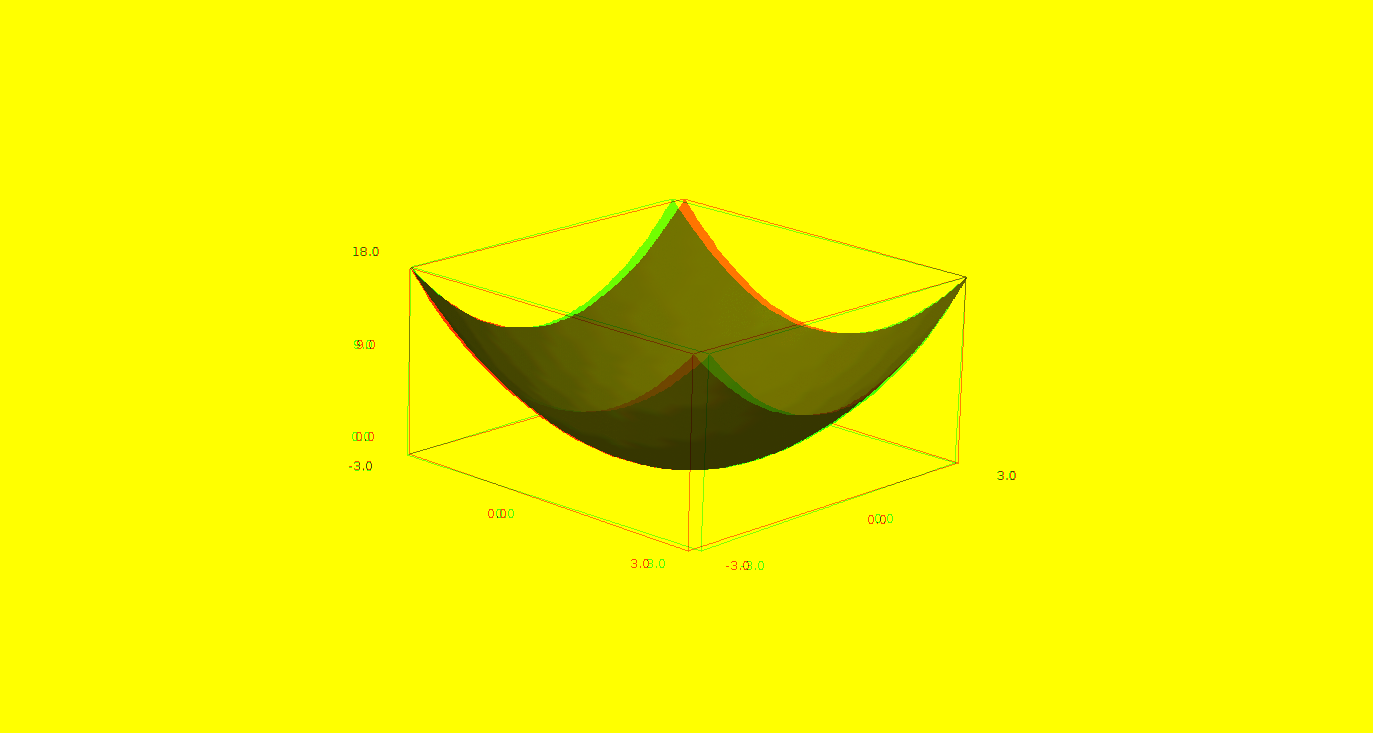
\includegraphics[width=15cm]{coupe.png}
        \else
            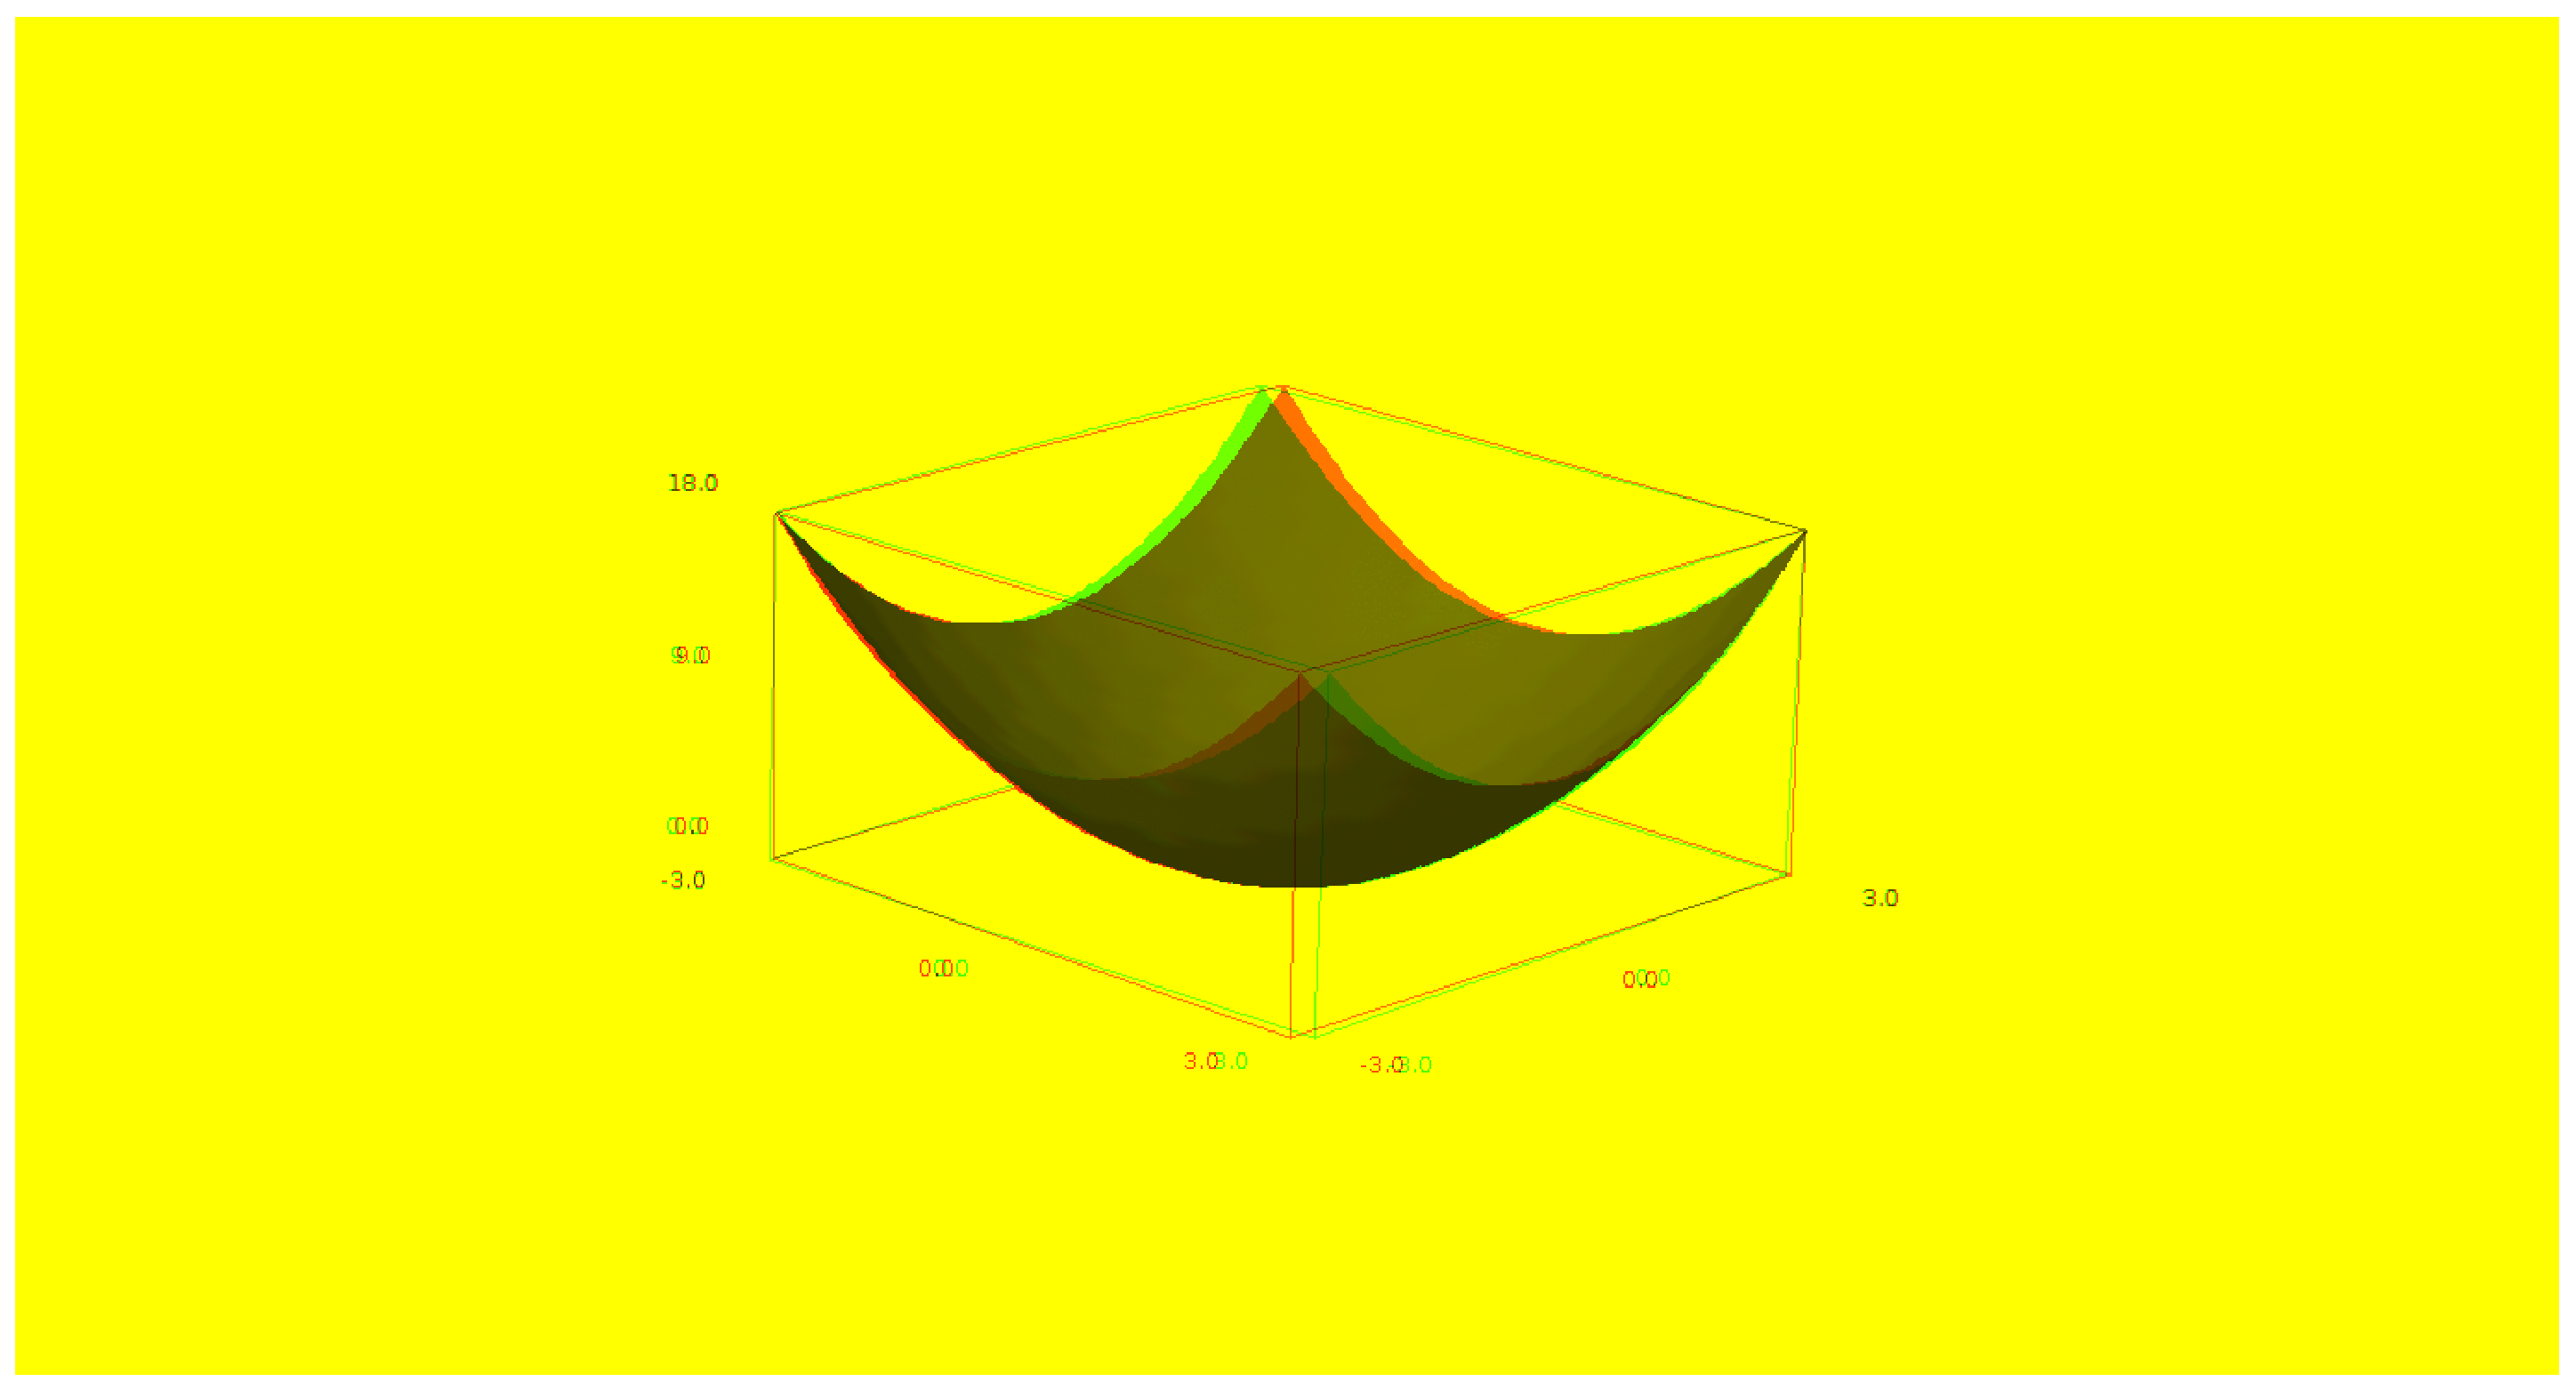
\includegraphics[width=15cm]{coupe.eps}
        \fi
    \end{center}
    À part que l'ordinateur l'a dit, est-ce qu'on peut comprendre pourquoi le graphe de la fonction $x^2+y^2$ ressemble à un bol ? En coordonnées cylindriques, le graphe s'écrit
    \begin{equation}
        z=r^2.
    \end{equation}
    Donc il se fait que plus on s'éloigne du point $(0,0)$ dans le plan $XY$, plus le graphe va monter. Et il monte à quelle vitesse ? Il monte à la vitesse $r^2$. Il s'agit donc de dessiner la fonction $z=r^2$ dans le plan et de la «faire tourner».

\end{example}

%+++++++++++++++++++++++++++++++++++++++++++++++++++++++++++++++++++++++++++++++++++++++++++++++++++++++++++++++++++++++++++
\section{Courbes de niveau}
%+++++++++++++++++++++++++++++++++++++++++++++++++++++++++++++++++++++++++++++++++++++++++++++++++++++++++++++++++++++++++++

Une technique utile pour se faire une idée de la forme d'une fonction en trois dimensions est de tracer les \defe{courbes de niveau}{courbe de niveau}. La courbe de niveau de hauteur $h$ est la courbe dans le plan donnée par l'équation
\begin{equation}
    f(x,y)=h.
\end{equation}

\begin{example}

    Dessinons par exemple les courbes de niveau de la fonction
    \begin{equation}
        f(x,y)=x+y+2.
    \end{equation}
    La courbe de niveau $h$ est donnée par l'équation $x+y+2=h$, c'est à dire
    \begin{equation}
        y(x)=-x+h-2.
    \end{equation}
    Par conséquent la courbe de niveau de hauteur $0$ est $y=-x-2$, celle de hauteur $5$ est $y=-x+3$, etc.
    
    Nous pouvons également nous aider de Sage pour ce faire :
    \begin{verbatim}
----------------------------------------------------------------------
| Sage Version 4.6.1, Release Date: 2011-01-11                       |
| Type notebook() for the GUI, and license() for information.        |
----------------------------------------------------------------------
sage: f(x,y)=x+y+2
sage: var('h')                   
h
sage: niveau(h,x)=solve(f(x,y)==h,y)[0].rhs()
sage: g1(x)=niveau(1,x)
sage: g1
x |--> -x - 1
    \end{verbatim}
    Ici la fonction \verb+g1+ est la courbe de niveau $1$. 

    Si on veut faire tracer une courbe de niveau, Sage peut le faire :
    \begin{verbatim}
        sage: implicit_plot(f(x,y)==1,(x,-3,3),(y,-4,4))
    \end{verbatim}
    Cela tracera la courbe de niveau $h=1$ dans la partie du plan $x\in\mathopen[ -3 , 3 \mathclose]$ et $y\in\mathopen[ -4,4 ,  \mathclose]$.
    
\end{example}

Il est bien entendu possible de créer automatiquement $50$ courbes de niveau et de demander de les tracer toutes sur le même graphe.
\VerbatimInput[tabsize=3]{courbeNiveau.py}

Le résultat est :

\begin{center}
    \ifpdf
        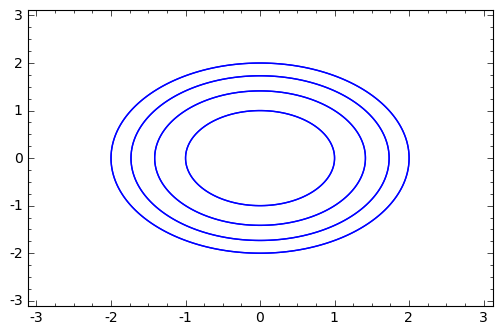
\includegraphics[width=8cm]{niveauCercles.png}
    \else
        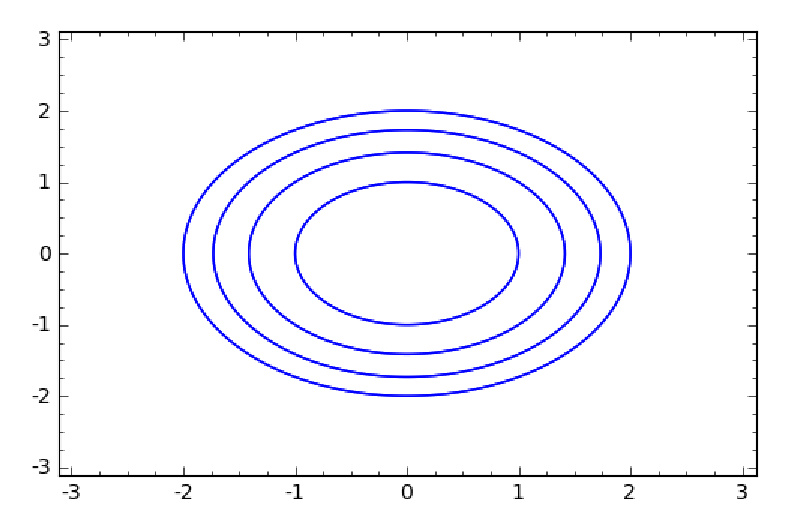
\includegraphics[width=8cm]{niveauCercles.eps}
    \fi
\end{center}
Notez que les courbes sont censées être des cercles : les axes $X$ et $Y$ n'ont pas la même échèle. Vous trouverez sur \href{http://uw.sagenb.org/home/pub/23/}{cette page} tout ce qu'il vous faudra pour créer des courbes de niveau avec Sage.

\begin{example}
    Un exemple plus riche en enseignements est celui de la fonction
    \begin{equation}
        f(x,y)=x^2-y^2.
    \end{equation}
    La courbe de niveau $h$ est donnée par l'équation $x^2-y^2=h$.

    Commençons par $h=0$. Dans ce cas nous avons $(x+y)(x-y)=0$ et par conséquent les courbes de niveau de hauteur zéro sont les deux droites $x+y=0$ et $x-y=0$.

    Voyons ensuite la courbe de niveau $h=1$. Cela est l'équation $x^2-y^2=1$, c'est à dire
    \begin{equation}
        y(x)=\pm\sqrt{x^2-1}.
    \end{equation}
    C'est une fonction qui n'est définie que pour $| x |\geq 1$. Avec $x=1$ nous avons $y=1$. Ensuite, lorsque $x$ grandit, $y$ grandit également, mais la courbe ne peut pas croiser la courbe de niveau $h=0$. Donc, suivant les notations de la figure \ref{LabelFigNiveauHyperbole}, la courbe de niveau «part» de $P$ et doit monter sans croiser les diagonales.

    \newcommand{\CaptionFigNiveauHyperbole}{La courbe de niveau $h=1$ de $x^2-y^2$. Notez qu'elle est en deux morceaux.}
    \input{Fig_NiveauHyperbole.pstricks}

    En ce qui concerne la courbe de niveau $h=-1$, elle correspond à la courbe $y=\pm\sqrt{1+x^2}$ qui est définie pour tous les $x\in\eR$. Le même raisonnement que précédemment nous amène à la figure \ref{LabelFigNiveauHyperboleDeux}.
\newcommand{\CaptionFigNiveauHyperboleDeux}{La courbe de niveau $x^2-y^2=-1$.}
\input{Fig_NiveauHyperboleDeux.pstricks}


\end{example}

Une autre façon de voir les courbe de niveau est de dire que la courbe de niveau de hauteur $h$ est la projection dans le plan $XY$ de la section du graphe de $f$ par le plan $z=h$.

On peut également définir le graphe de fonctions de trois (ou plus) variables. Le graphe de la fonction $f\colon D\subset\eR^3\to \eR$ est l'ensemble
\begin{equation}
    \big\{ \big( x,y,z,f(x,y,z) \big)\tq (x,y,z)\in D \big\}\subset \eR^4.
\end{equation}
De tels graphes ne peuvent pas être représentés sur une feuille de papier. Il est toutefois possible de définir les ensembles de niveaux :
\begin{equation}
    E_h=\big\{ (x,y,z)\in D\tq  f(x,y,z)=h\big\}.
\end{equation}
Ce sont des surfaces dans $\eR^3$ que l'on peut dessiner.

\begin{example}
    Les surfaces de niveau de la fonction $f(x,y,z)=x^2+y^2+z^2$ sont des sphères. Il n'y a pas de surfaces de niveau pour les «hauteurs» négatives.
\end{example}

\begin{example}
    Considérons la fonction $f(x,y,z)=x^2+y^2-z^2$. En coordonnées cylindrique, cette fonction s'écrit
    \begin{equation}
        f(r,\theta,z)=r^2-z^2.
    \end{equation}
    La surface de niveau $0$ est donnée par l'équation $r=| z |$. Cela fait un cercle à chaque hauteur, dont le rayon grandit linéairement avec la hauteur; le tout est donc un cône. C'est d'ailleurs le cône obtenu par rotation de la courbe de niveau $h=0$ que nous avions obtenue pour la fonction $x^2-y^2$.

    En ce qui concerne les ensembles de niveau positifs, ils sont donnés par
    \begin{equation}
        z=\pm\sqrt{x^2+y^2-h}.
    \end{equation}
    Notez qu'ils ne sont pas définis pour $r\geq h$. Cela pose un petit problème quand on veut le tracer à l'ordinateur :
    \begin{verbatim}
----------------------------------------------------------------------
| Sage Version 4.6.1, Release Date: 2011-01-11                       |
| Type notebook() for the GUI, and license() for information.        |
----------------------------------------------------------------------
sage: var('x,y')
(x, y)
sage: f(x,y)=sqrt(x**2+y**2-3)
sage: F=plot3d(f(x,y),(x,-5,5),(y,-5,5)) 
sage: G=plot3d(-f(x,y),(x,-5,5),(y,-5,5))    
sage: F+G
    \end{verbatim}
Le résultat est\footnote{Encore une fois : ça donne mieux à l'écran, et vous pouvez le faire bouger; je vous encourage à le faire !} :
    \begin{center}
        \ifpdf
            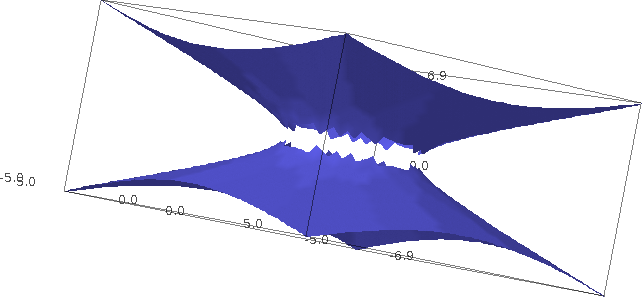
\includegraphics[width=15cm]{AdSmauvais.png}
        \else
            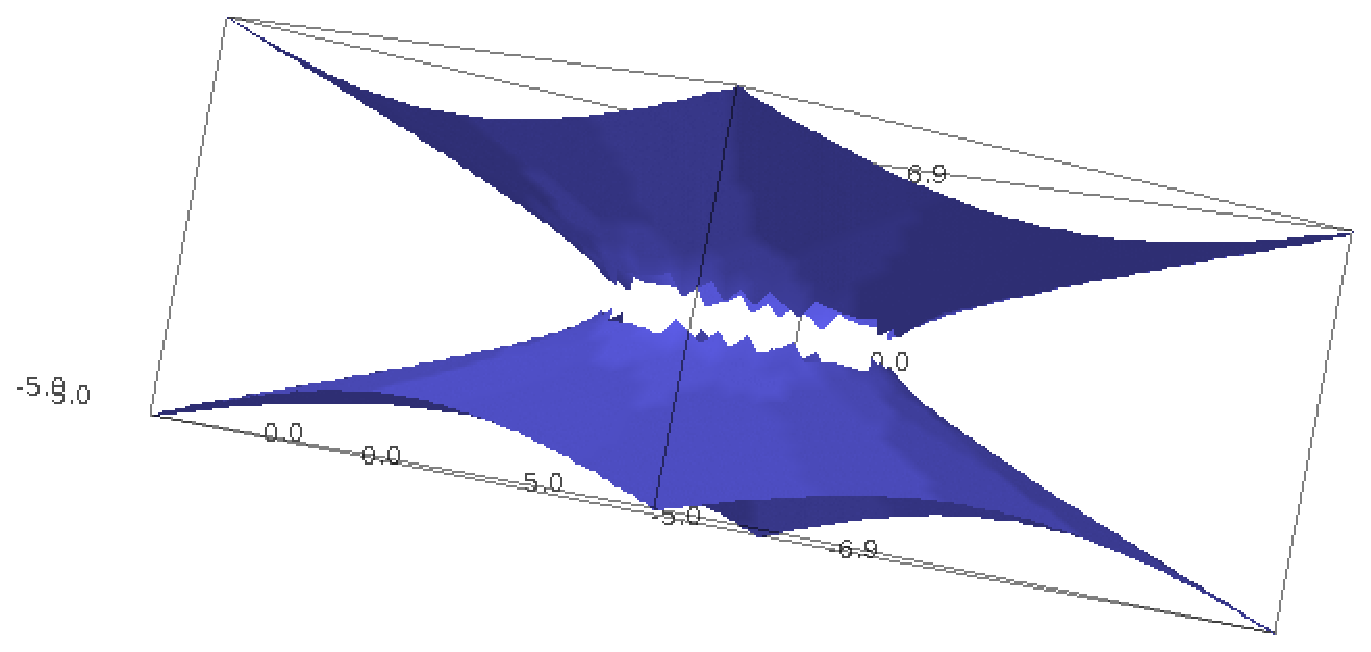
\includegraphics[width=15cm]{AdSmauvais.eps}
        \fi
    \end{center}
    On voit qu'il y a un grand trou au centre correspondant aux $z$ proches de zéro. Or d'après l'équation, il n'en est rien : en $z=0$ il y a bel et bien tout un cercle. Afin d'obtenir une meilleur image, il faut demander de tracer avec un maillage plus fin :
    \begin{verbatim}
----------------------------------------------------------------------
| Sage Version 4.6.1, Release Date: 2011-01-11                       |
| Type notebook() for the GUI, and license() for information.        |
----------------------------------------------------------------------
sage: var('x,y')
(x, y)
sage: f(x,y)=sqrt(x**2+y**2-3)
sage: F=plot3d(f(x,y),(x,-5,5),(y,-5,5),plot_points=300) 
sage: G=plot3d(-f(x,y),(x,-5,5),(y,-5,5),plot_points=300)
sage: F+G
    \end{verbatim}
    Le temps de calcul est un peu plus long, mais le résultat est meilleur :
    \begin{center}
        \ifpdf
            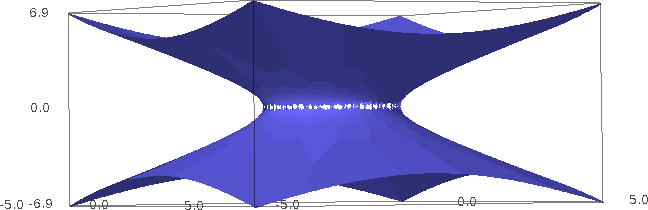
\includegraphics[width=15cm]{AdSbon.png}
        \else
            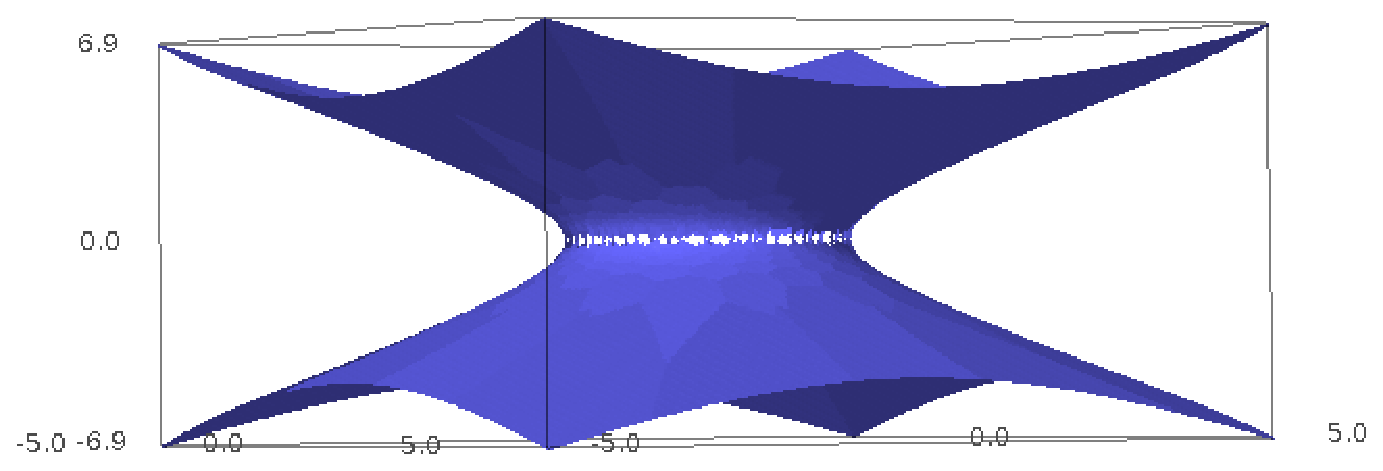
\includegraphics[width=15cm]{AdSbon.eps}
        \fi
    \end{center}
\end{example}

%+++++++++++++++++++++++++++++++++++++++++++++++++++++++++++++++++++++++++++++++++++++++++++++++++++++++++++++++++++++++++++
\section{Dérivées partielles}
%+++++++++++++++++++++++++++++++++++++++++++++++++++++++++++++++++++++++++++++++++++++++++++++++++++++++++++++++++++++++++++

Soit $f\colon \eR^2\to \eR$ une fonction de deux variables et soit $(a,b)\in\eR^2$. La façon la plus naturelle de définir une dérivée à deux variables est de considérer les \defe{dérivées partielles}{dérivée!partielle} définies par
\begin{equation}
    \begin{aligned}[]
        \frac{ \partial f }{ \partial x }(a,b)&=\lim_{x\to a} \frac{ f(x,b)-f(a,b) }{ x-a }\\
        \frac{ \partial f }{ \partial y }(a,b)&=\lim_{y\to b} \frac{ f(a,y)-f(a,b) }{y-b}.
    \end{aligned}
\end{equation}
Ces nombres représentent la façon dont le nombre $f(x,y)$ varie lorsque soit seul $x$ varie soit seul $y$ varie. Les dérivées partielles se calculent de la même façon que les dérivées normales. Pour calculer $\partial_xf$, on fait «comme si» $y$ était une constante, et pour calculer $\partial_yf$, on fait comme si $x$ était une constante.

\begin{example}
    Considérons $f(x,y)=x^2y+y^2 e^{x}$. Les dérivées partielles sont
    \begin{equation}
        \begin{aligned}[]
            \frac{ \partial f }{ \partial x }&=2xy+y^2e^x\\
            \frac{ \partial f }{ \partial y }&=x^2+2ye^x.
        \end{aligned}
    \end{equation}
\end{example}

Cet exemple était l'exemple facile où tout se passe bien.

\begin{example}
    Les choses sont moins simples lorsqu'on considère la fonction suivante :
    \begin{equation}
        f(x,y)=\begin{cases}
            \frac{ xy }{ x^2+y^2 }    &   \text{si $(x,y)\neq(0,0)$}\\
            0    &    \text{si $(x,y)=(0,0)$}.
        \end{cases}
    \end{equation}
    On voit que pour tout $x$ et tout $y$, nous avons $f(x,0)=f(0,y)=0$. Donc cette fonction est nulle sur les axes horizontaux et verticaux. Nous avons en particulier
    \begin{equation}
        \begin{aligned}[]
            \frac{ \partial f }{ \partial x }(0,0)&=0\\
            \frac{ \partial f }{ \partial y }(0,0)&=0.
        \end{aligned}
    \end{equation}
    Donc ces dérivées partielles existe.

    Il n'est par contre pas question de dire que cette fonction «va bien» autour du point $(0,0)$. En effet si nous regardons sa valeur sur la droite diagonale $y=x$, nous avons
    \begin{equation}
        f(x,x)=\frac{ x^2 }{ 2x^2 }=\frac{ 1 }{2}.
    \end{equation}
    Par conséquent si nous suivons la fonction le long de la droite $y=x$, la hauteur vaut $\frac{ 1 }{2}$ en permanence, saut juste en $(0,0)$ où la fonction fait un grand plongeon !
    \begin{verbatim}
    sage: var('x,y')
    (x, y)
    sage: f(x,y)=(x*y)/(x**2+y**2)
    sage: plot3d(f,(x,-2,2),y(-2,2))
    \end{verbatim}

    D'ailleurs elle fait un plongeon le long de toutes les droites (sauf verticale et horizontale). En effet si nous regardons la fonction le long de la droite $y=mx$, nous avons
    \begin{equation}
        f(x,mx)=\frac{ mx^2 }{ x^2+m^2x^2 }=\frac{ m }{ 1+m^2 }.
    \end{equation}
    La fonction est donc \emph{constante} sur chacune de ces droites. Il n'est donc pas question de dire que cette fonction est «dérivable» en $(0,0)$, vu qu'elle fait des grands sauts dans presque toutes les directions.
\end{example}

Nous devons donc trouver mieux que les dérivées partielles pour étudier le comportement des fonctions un peu problématiques.

Nous nous souvenons de l'équation \eqref{EqCodeDerviffxam} qui nous dis que pour une fonction d'une variable la dérivabilité signifiait qu'il existait un nombre $\ell$ et une fonction $\alpha$ tels
\begin{equation}
    f(x)=f(a)+\ell(x-a)+(x-a)\alpha(x-a)
\end{equation}
et $\lim_{t\to 0} \alpha(t)=0$. 

En nous inspirant de cela, nous posons la définition suivante.
\begin{definition}      \label{DefDiffabel}
    Une fonction $f\colon \eR^2\to \eR$ est \defe{différentiable}{différentiable} au point $(a,b)\in\eR^2$ si il existe deux nombres $\ell_1$, $\ell_2$ ainsi qu'une fonction $\alpha$ tels que
    \begin{equation}\label{EqCondDiffabel}
        \begin{aligned}[]
            f(x,y)=f(a,b)&+\ell_1(x-a)+\ell_2(y-b)\\
                    &+\sqrt{(x-a)^2+(y-b)^2}\alpha\big( \sqrt{(x-a)^2+(y-b)^2} \big).
        \end{aligned}
    \end{equation}
\end{definition}

En utilisant la notation vectorielle, cela peut être écrite sous forme très compacte. Posons
\begin{equation}
    \begin{aligned}[]
        \ell&=\begin{pmatrix}
            \ell_1    \\ 
            \ell_2    
        \end{pmatrix},&
        X&=\begin{pmatrix}
            x    \\ 
            y    
        \end{pmatrix},&
        P&=\begin{pmatrix}
            a    \\ 
            b    
        \end{pmatrix}.
    \end{aligned}
\end{equation}
Alors la condition \eqref{EqCondDiffabel} s'écrit
\begin{equation}
    f(X)=f(P)+\ell\cdot(X-P)+\| X-P \|\alpha\big( \| X-P \| \big).
\end{equation}

\begin{proposition}
    Si $f$ est différentiable en $(a,b)$, alors les nombres $\partial_xf(a,b)$ et $\partial_yf(a,b)$ existent et valent respectivement $\ell_1$ et $\ell_2$.
\end{proposition}

\begin{proof}
    Afin de calculer la dérivée partielle dans la direction de $x$, nous posons $y=b$ dans la condition \eqref{EqCondDiffabel} :
    \begin{equation}
        f(x,b)=f(a,b)+\ell_1(x-a)+| x-a |\alpha\big( | x-a | \big),
    \end{equation}
    et donc
    \begin{equation}
        \frac{ f(x,b)-f(a,b) }{ x-a }=\ell_1\pm\alpha\big( | x-a | \big).
    \end{equation}
    Ici le $\pm$ est parce que nous avons divisé $(x-a)$ par $| x-a |$. Quel que soit ce signe, de toutes façons la limite du membre de droite lorsque $x$ tend vers $a$ est $\ell_1$ parce que $\lim_{x\to a} \alpha(| x-a |)=0$.

    Afin de prouver l'existence de la dérivée dans la direction de $y$, nous procédons de la même manière, mais en partant de $f(a,y)$.
\end{proof}

\begin{proposition}
    Si $f$ est différentiable au point $(a,b)$, alors elle y est continue, c'est à dire que
    \begin{equation}
        \lim_{(x,y)\to(a,b)}f(x,y)=f(a,b).
    \end{equation}
\end{proposition}

\begin{proof}
    Si nous considérons la différence entre $f(x,y)$ et $f(a,b)$, nous avons (en notations matricielle) :
    \begin{equation}
        | f(X)-f(P) |=| \ell\cdot(X-P)+\| X-P \|\alpha(\| X-P \|) |.
    \end{equation}
    Le membre de droite tend évidemment vers zéro lorsque $X$ tend vers $P$.
\end{proof}
    \begin{remark}
        Attention : ceci n'est pas une preuve. En effet, dans la mesure où nous n'avons même pas donné de définition de la limite, il n'est pas possible de donner une \emph{vraie} preuve de quoi que ce soit. 
    \end{remark}

Nous avons vu que l'existence des deux dérivées partielles ne permettait pas de conclure à la différentiabilité. La différentiabilité d'une fonction peut néanmoins être déduites d'une étude plus précise des dérivées partielles. Nous avons pour cela les propositions \ref{PropExistDiffUn} et \ref{PropExistDiffDeux}

\begin{proposition} \label{PropExistDiffUn}
    Soit $f$ une fonction de $x$ et $y$ et un point $(a,b)\in\eR^2$. Si les nombres $\partial_xf(a,b)$ et $\partial_yf(a,b)$ existent et si il existe une fonction $\alpha\colon \eR\to \eR$ telle que
    \begin{equation}        \label{eqCritDifffabsrt}
        \begin{aligned}[]
            f(x,y)=f(a,b)&+\frac{ \partial f }{ \partial x }(a,b)(x-a)+\frac{ \partial f }{ \partial y }(a,b)(y-b)\\
            &+\| (x,y)-(a,b) \| \alpha\Big( \| (x,y)-(a,b) \| \Big)
        \end{aligned}
    \end{equation}
    et
    \begin{equation}
        \lim_{t\to 0} \alpha(t)=0,
    \end{equation}
    alors $f$ est différentiable en $(a,b)$.
\end{proposition}
Dans cet énoncé nous avons écrit $d\big( (x,y),(a,b) \big)$ la distance entre $(x,y)$ et $(a,b)$, c'est à dire le nombre $\sqrt{(x-a)^2+(y-b)^2}$. Afin d'écrire l'équation \eqref{eqCritDifffabsrt} sous forme plus compacte, nous introduisons le vecteur
\begin{equation}
    \nabla f(a,b)=\begin{pmatrix}
        \frac{ \partial f }{ \partial x }(a,b)    \\ 
        \frac{ \partial f }{ \partial y }(a,b).    
    \end{pmatrix}
\end{equation}
L'équation \eqref{eqCritDifffabsrt} devient alors
\begin{equation}        \label{EqdiffComp}
    f(X)=f(P)+\nabla f(a,b)\cdot (X-P)+\| X-P \|\alpha\big( \| X-P \| \big).
\end{equation}
Le vecteur $\nabla f(a,b)$ est appelé le \defe{gradient}{gradient} de $f$ au point $(a,b)$.


\begin{proposition} \label{PropExistDiffDeux}
    Soit $f$ une fonction de deux variables admettant des dérivées partielles $\partial_xf(x,y)$ et $\partial_yf(x,y)$ qui sont elles-mêmes des fonctions continues de $x$ et $y$. Alors la fonction $f$ est différentiable partout.
\end{proposition}

\begin{remark}
    Tout ce qui a été dit, et tout ce qui sera dit, sur les fonctions a deux variables se généralise immédiatement aux fonctions à plus de variables. C'est dans ce but que la notation «compacte» utilisant les vecteurs est très pratique.
\end{remark}

Si nous remplaçons les accroissements $x-a$ et $y-b$ par $h$ et $k$, le critère de différentiabilité s'écrit
\begin{equation}
    \begin{aligned}[]
        f(a+h,b+k)=f(a,b)+\frac{ \partial f }{ \partial x }(a,b)h&+\frac{ \partial f }{ \partial y }(a,b)k\\
        &+\sqrt{h^2+k^2}\alpha\big( \sqrt{h^2+k^2} \big).
    \end{aligned}
\end{equation}
Le dernier terme du membre de droite tend vers zéro à une vitesse double lorsque $h$ et $k$ tendent vers zéro : d'une part parce que $\sqrt{h^2+k^2}$ tend vers zéro et d'autre part parce que $\alpha\big( \sqrt{h^2+k^2} \big)$ tend vers zéro. Nous avons donc la «bonne» approximation
\begin{equation}        \label{EqFormApproxfxyab}
    f(x,y)\simeq f(a,b)+\frac{ \partial f }{ \partial x }(a,b)(x-a)+\frac{ \partial f }{ \partial y }(a,b)(y-b).
\end{equation}
lorsque $(x,y)$ n'est pas trop loin de $(a,b)$. Cette expression est évidemment une généralisation immédiate de l'équation \eqref{EqfxdxSimeqfxfpx}. Elle exprime que l'on peut obtenir des information sur la valeur d'une fonction en $(x,y)$ si on peut calculer la fonction et ses dérivées en un point $(a,b)$ non loin de $(x,y)$.

Cette formule peut aussi être vue sous la forme suivante, plus pratique dans certains calculs :
\begin{equation}        \label{EqFormApproxfxyabDF}
    f(a+\Delta x,b+\Delta y)\simeq f(a,b)+\Delta x\frac{ \partial f }{ \partial x }(a,b)+\Delta y\frac{ \partial f }{ \partial y }(a,b).
\end{equation}

\begin{example}
    Prenons la fonction $f(x,y)=\cos(x)\sin(y)$ et calculons une approximation de
    \begin{equation}
        f\big( \frac{ \pi }{ 3 }+0.01,\frac{ \pi }{ 2 }+0.03 \big).
    \end{equation}
    D'abord les dérivées partielles sont
    \begin{equation}
        \begin{aligned}[]
            \frac{ \partial f }{ \partial x }(x,y)=-\sin(x)\sin(y)\\
            \frac{ \partial f }{ \partial y }(x,y)=\cos(x)\cos(y).
        \end{aligned}
    \end{equation}
    Nous allons utiliser l'approximation
    \begin{equation}
        f\big( \frac{ \pi }{ 3 }+0.01,\frac{ \pi }{ 2 }+0.03 \big)\simeq f\big( \frac{ \pi }{ 3 },\frac{ \pi }{2} \big)+0.01\frac{ \partial f }{ \partial x }\big( \frac{ \pi }{ 3 },\frac{ \pi }{2} \big)+0.03\frac{ \partial f }{ \partial y }\big( \frac{ \pi }{ 3 },\frac{ \pi }{2} \big).
    \end{equation}
    Nous avons
    \begin{equation}
        \begin{aligned}[]
            \frac{ \partial f }{ \partial x }\big( \frac{ \pi }{ 3 },\frac{ \pi }{2} \big)&=-\sin\frac{ \pi }{ 3 }\sin\frac{ \pi }{ 2 }=-\frac{ \sqrt{3} }{2}\\
            \frac{ \partial f }{ \partial y }\big( \frac{ \pi }{ 3 },\frac{ \pi }{2} \big)&=\cos\frac{ \pi }{ 3 }\cos\frac{ \pi }{ 2 }=0.
        \end{aligned}
    \end{equation}
    Par conséquent
    \begin{equation}
        f\big( \frac{ \pi }{ 3 }+0.01,\frac{ \pi }{ 2 }+0.03 \big)\simeq \frac{ 1 }{2}-0.01\frac{ \sqrt{3} }{2}=\frac{ 1 }{2}-\frac{ \sqrt{3} }{ 200 }. 
    \end{equation}
    
    \begin{verbatim}
sage: var('x,y')
(x, y)
sage: f(x,y)=cos(x)*sin(y)
sage: a=f(pi/3+0.01,pi/2+0.03)
sage: numerical_approx(a)
0.491093815387986
sage: b=1/2-sqrt(3)/200
sage: numerical_approx(b)
0.491339745962156
sage: numerical_approx(a-b)
-0.000245930574169814
    \end{verbatim}
    Cela fait une erreur de l'ordre du dix millième. 
    
\end{example}

\begin{remark}
    Les esprits les plus critiques diront que cette vérification pas Sage n'en est pas une parce que Sage a certainement utilisé un algorithme d'approximation qui se base sur la même idée que ce que nous venons de faire, et que par conséquent le fait qu'il obtienne le même résultat que nous est un peu tautologique. 
    
    Ils n'auront pas tord. Cependant, le code source de Sage est disponible publiquement\footnote{Voir \url{http://www.sagemath.org}}; vous pouvez aller le lire et vérifier qu'il y a effectivement une \emph{preuve} que le résultat fourni par Sage possède une bonne dizaine de décimales correctes. 
    
    Cette disponibilité publique du code source est une des nombreuses différence fondamentale entre Sage et votre calculatrice\footnote{et les autres logiciels de type fenêtre, pomme ou feuille d'érable.}. Dois-je vous rappeler qu'un des principes fondamentaux de l'éthique scientifique est que les résultats et les méthodes utilisées doivent être absolument ouverts à la vérification et à la critique de tous ?
\end{remark}

%---------------------------------------------------------------------------------------------------------------------------
\subsection{Différentielle}
%---------------------------------------------------------------------------------------------------------------------------

\begin{definition}      \label{DefDiffrdrr}
    Lorsque $f$ est différentiable au point $(a,b)$, on appelle \defe{différentielle}{différentielle} de $f$ l'application linéaire
    \begin{equation}        \label{EqDefDiffmapdf}
        \begin{aligned}
            df_{(a,b)}\colon \eR^2&\to \eR \\
            \begin{pmatrix}
                u_1    \\ 
                u_2    
            \end{pmatrix}&\mapsto \frac{ \partial f }{ \partial x }(a,b)u_1+\frac{ \partial f }{ \partial y }(a,b)u_2. 
        \end{aligned}
    \end{equation}
    En notations compacte :
    \begin{equation}        \label{EqdfUPnable}
        df_{P}(U)=\nabla f(P)\cdot U.
    \end{equation}
\end{definition}

Note : dans la suite nous allons rendre notre «notation compacte» plus agréable à lire en abandonnant les majuscules. L'équation \eqref{EqdfUPnable} s'écrira donc
\begin{equation}        \label{Eqdfpunfpdu}
    df_p(u)=\nabla f(p)\cdot u.
\end{equation}


%+++++++++++++++++++++++++++++++++++++++++++++++++++++++++++++++++++++++++++++++++++++++++++++++++++++++++++++++++++++++++++
\section{Plan tangent au graphe d'une fonction}
%+++++++++++++++++++++++++++++++++++++++++++++++++++++++++++++++++++++++++++++++++++++++++++++++++++++++++++++++++++++++++++

Nous avons vu que, de la même façon qu'en deux dimensions nous avions l'approximation \eqref{Eqfxsimesfa} d'une fonction par sa tangente, en trois dimensions nous avons l'approximation suivante d'une fonction de deux variables :
\begin{equation}
    f(x,y)\simeq f(a,b)+\frac{ \partial f }{ \partial x }(a,b)(x-a)+\frac{ \partial f }{ \partial y }(a,b)(y-b)
\end{equation}
lorsque $(x,y)$ n'est pas trop loin de $(a,b)$. Cela signifie que le graphe de $f$ ressemble au graphe de la fonction $T_{(a,b)}$ donnée par
\begin{equation}
    T_{(a,b)}(x,y)=f(a,b)+\frac{ \partial f }{ \partial x }(a,b)(x-a)+\frac{ \partial f }{ \partial y }(a,b)(x-a).
\end{equation}
En notations compactes :
\begin{equation}
    T_p(x)=f(p)+\nabla f(p)\cdot (x-p).
\end{equation}
Le graphe de la fonction $T_p$ sera le \defe{plan tangent}{plan tangent} au graphe de $f$ au point $p$. L'équation du plan tangent sera donc
\begin{equation}
    z-f(p)=\nabla f(p)\cdot (x-p).
\end{equation}

\begin{remark}
    Lorsque nous utilisons la notation vectorielle, la lettre «$x$» désigne le vecteur $(x,y)$. Il faut être attentif. Dans un cas $x$ est un vecteur dans l'autre c'est une composante d'un vecteur.
\end{remark}




%+++++++++++++++++++++++++++++++++++++++++++++++++++++++++++++++++++++++++++++++++++++++++++++++++++++++++++++++++++++++++++
\section{Dérivée directionnelle}
%+++++++++++++++++++++++++++++++++++++++++++++++++++++++++++++++++++++++++++++++++++++++++++++++++++++++++++++++++++++++++++

Nous sommes capables de dériver une fonction de deux variables $f(x,y)$ par rapport à $x$ et par rapport à $y$. C'est à dire que nous sommes capables de donner la variation de la fonction lorsqu'on bouge le long des axes horizontal et vertical. Il est évidemment souhaitable de parler de la variation de la fonction lorsqu'on se déplace le long d'autre droites.

Soit donc $u=\begin{pmatrix}
    u_1    \\ 
    u_2    
\end{pmatrix}$ un vecteur unitaire (c'est à dire $u_1^2+u_2^2=1$), et considérons la fonction de une variable
\begin{equation}
    \begin{aligned}
        \varphi\colon \eR&\to \eR \\
        t&\mapsto f(a+tu_1,b+tu_2). 
    \end{aligned}
\end{equation}
La fonction $\varphi$ n'est rien d'autre que la fonction $f$ vue le long de la droite de direction donnée par le vecteur $u$. Nous pouvons aussi l'écrire $\varphi(t)=f(p+tu)$.

\begin{proposition}
    Si $f$ est différentiable en $(a,b)$ alors la fonction $\varphi$ est dérivable en $0$ et on a
    \begin{equation}
        \varphi'(0)=\nabla f(p)\cdot u
    \end{equation}
    où nous avons noté $p=(a,b)$.
\end{proposition}

\begin{proof}
    Récrivons la formule \eqref{EqdiffComp} sous la forme
    \begin{equation}
        f(x)=f(p)+\nabla f(p)\cdot (x-p)+\| x-p \|\alpha(\| x-p \|).
    \end{equation}
    Cela étant vrai pour tout $x$, nous l'écrivons en particulier pour $x=p+tu$ où $t$ est un réel et $u$ est le vecteur unitaire choisi. Nous avons donc
    \begin{equation}
        f(p+tu)=f(p)+t\nabla f(p)\cdot u+\| tu \|\alpha(\| tu \|).
    \end{equation}
    En utilisant le fait que $u$ est unitaire, $\| tu \|=| t |\| u \|=| t |$. La dérivée de $\varphi$ en $0$ est alors donnée par
    \begin{equation}
        \lim_{t\to 0} \frac{ f(p+tu)-f(p) }{ t }=\lim_{t\to 0} \nabla f(p)\cdot u+\alpha(| t |).    
    \end{equation}
    Lorsque nous prenons la limite, le membre de gauche devient $\varphi'(0)$ tandis que dans le membre de droite, le second terme disparaît. Nous avons finalement
    \begin{equation}
        \varphi'(0)=\nabla f(p)\cdot u
    \end{equation}
\end{proof}

\begin{definition}
    Le nombre
    \begin{equation}
        \lim_{t\to 0} \frac{ f\big( a+tu_1,b+tu_2 \big)-f(a,b) }{ t }
    \end{equation}
    est la \defe{dérivée directionnelle}{dérivée!directionnelle} de $f$ dans la direction de $u$ au point $(a,b)$. Il sera noté
    \begin{equation}
        \frac{ \partial f }{ \partial u }(a,b),
    \end{equation}
    ou plus simplement $\partial_uf(a,b)$.
\end{definition}

Lorsque $f$ est différentiable, la dérivée directionnelle est donnée par
\begin{equation}        \label{EqDerDirnablau}
    \frac{ \partial f }{ \partial u }(p)=\nabla f(p)\cdot u.
\end{equation}

En combinant avec l'équation \eqref{Eqdfpunfpdu}, nous avons la suite d'égalités
\begin{equation}        \label{Eqsuitedfnfdsdfu}
    df_p(u)=\nabla f(p)\cdot u=\frac{ \partial f }{ \partial x }(p)u_1+\frac{ \partial f }{ \partial y }(p)u_2+\frac{ \partial f }{ \partial z }(p)u_3=\frac{ \partial f }{ \partial u }(p).
\end{equation}
La dernière équation est seulement vraie si $\| u \|=1$.

%---------------------------------------------------------------------------------------------------------------------------
\subsection{Gradient : direction de plus grande pente}
%---------------------------------------------------------------------------------------------------------------------------

Étant donné que $u$ est de norme $1$, l'inégalité de Cauchy-Schwartz donne
\begin{equation}
    \big| \nabla f(a,b)\cdot \begin{pmatrix}
        u_1    \\ 
        u_2    
    \end{pmatrix}\big|\leq \| \nabla f(a,b) \|.
\end{equation}
Donc
\begin{equation}
    -\| \nabla f(p) \|\leq \nabla f(p)\cdot u\leq\| \nabla f(p) \|.
\end{equation}
La norme de la dérivée directionnelle (qui est la valeur absolue du nombre au centre) est donc «coincée» entre $-\| \nabla f(p) \|$ et $\| \nabla f(p) \|$. Prenons par exemple
\begin{equation}
    u=\frac{ \nabla f(p) }{ \| \nabla f(p) \| }.
\end{equation}
Dans ce cas, nous avons exactement
\begin{equation}
    \nabla f(p)\cdot u=\| \nabla f(p) \|,
\end{equation}
qui est la valeur maximale que la dérivée directionnelle peut prendre.

La direction du gradient est donc la direction suivant laquelle la dérivée directionnelle est la plus grande. Pour la même raison, la dérivée directionnelle est la plus petite dans le sens opposé au gradient.

En termes bien clairs : lorsqu'on veut aller le plus vite possible au ski, on prend la direction du gradient de la piste de ski. C'est dans cette direction que ça descend le plus vite. Dans quelle direction vont les débutants ? Ils vont perpendiculairement à la pente (ce qui ennuie tout le monde, mais c'est un autre problème). Les débutants vont donc dans la direction perpendiculaire au gradient. Prenons donc $u\perp \nabla f(p)$ et calculons la dérivée directionnelle de $f$ dans la direction $u$ en utilisant la formule \ref{EqDerDirnablau} :
\begin{equation}
    \frac{ \partial f }{ \partial u }(p)=\nabla f(p)\cdot u=0
\end{equation}
parce que nous avons choisit $u\perp \nabla f(p)$. Nous voyons donc que les débutants en ski ont eu la bonne intuition que la direction dans laquelle la piste ne descend pas, c'est la direction perpendiculaire au gradient.

C'est aussi pour cela que l'on a tendance à faire du zig-zag à vélo lorsqu'on monte une pente très forte et qu'on est fatigué. C'est toujours pour cela que les routes de montagne font de longs lacets. La montée est moins rude en suivant une direction proche d'être perpendiculaire au gradient !

\begin{theorem}
    Le gradient des fonction suit à peu près les mêmes règles que les dérivées. Soient $f$ et $g$ deux fonctions différentiables. Nous avons entre autres
    \begin{enumerate}
        \item
            $\nabla(f+g)=\nabla f+\nabla g$;
        \item
            $\nabla(fg)(a,b)=g(a,b)\nabla f(a,b)+f(a,b)\nabla g(a,b)$;
        \item
            Dès que $g(a,b)\neq 0$, nous avons
            \begin{equation}
                \nabla\frac{ f }{ g }=\frac{ g(a,b)\nabla f(a,b)-f(a,b)\nabla g(a,b) }{ g(a,b)^2 }.
            \end{equation}
    \end{enumerate}
\end{theorem}



\chapter{Champs de vecteurs}
% This is part of Mes notes de mathématique
% Copyright (c) 2011-2012,2015
%   Laurent Claessens
% See the file fdl-1.3.txt for copying conditions.

Les champs de vecteurs et tout ce qui s'y rapportent jouent un rôle crucial en électromagnétisme. Voir par exemple \cite{Schomblond_em}.

%+++++++++++++++++++++++++++++++++++++++++++++++++++++++++++++++++++++++++++++++++++++++++++++++++++++++++++++++++++++++++++
\section{Les fonctions à valeurs vectorielles}
%+++++++++++++++++++++++++++++++++++++++++++++++++++++++++++++++++++++++++++++++++++++++++++++++++++++++++++++++++++++++++++

Jusqu'à présent nous avons vu des fonctions de plusieurs variables qui prenaient leurs valeurs dans $\eR$. Nous allons maintenant voir ce qu'il se passe lorsque les fonctions prennent leurs valeurs dans $\eR^3$.

Une fonction d'une variable est dite \defe{à valeurs vectorielles}{fonction!valeurs vectorielles} lorsque
\begin{equation}
    \begin{aligned}
        f\colon I\subset \eR&\to \eR^3 \\
        f(x)&=\begin{pmatrix}
            f_1(x)    \\ 
            f_2(x)    \\ 
            f_3(x)    
        \end{pmatrix}.
    \end{aligned}
\end{equation}
Les fonctions $f_i\colon \eR\to \eR$ sont les \defe{composantes}{composante} de $f$. Ce que nous avons raconté à propos des dérivées passe facilement :
\begin{equation}
    \frac{ f(a+\epsilon)-f(a) }{ \epsilon }=
    \begin{pmatrix}
        \frac{ f_1(a+\epsilon)-f_1(a) }{ \epsilon }    \\ 
        \frac{ f_2(a+\epsilon)-f_2(a) }{ \epsilon }    \\ 
        \frac{ f_3(a+\epsilon)-f_3(a) }{ \epsilon }    
    \end{pmatrix}.
\end{equation}
En particulier dès que les fonctions $f_i$ sont dérivables, nous avons
\begin{equation}
    f'(a)=\begin{pmatrix}
        f_1'(a)    \\ 
        f_2'(a)    \\ 
        f_3'(a)    
    \end{pmatrix}
\end{equation}
comme dérivée de la fonction. Cette dérivée est un vecteur.

\begin{example}
    Si
    \begin{equation}
        f\colon x\in\eR\mapsto \begin{pmatrix}
            x^2 e^{x}    \\ 
            \cos(x^2)    \\ 
            x^3+x    
        \end{pmatrix},
    \end{equation}
    alors
    \begin{equation}
        f'(x)=\begin{pmatrix}
            2xe^x+x^2e^x    \\ 
            -2x\sin(x^2)    \\ 
            3x^2+1    
        \end{pmatrix}.
    \end{equation}
\end{example}

%+++++++++++++++++++++++++++++++++++++++++++++++++++++++++++++++++++++++++++++++++++++++++++++++++++++++++++++++++++++++++++
\section{Fonctions vectorielles de plusieurs variables}
%+++++++++++++++++++++++++++++++++++++++++++++++++++++++++++++++++++++++++++++++++++++++++++++++++++++++++++++++++++++++++++

Ce sont les fonctions de la forme
\begin{equation}
    \begin{aligned}
        f\colon \eR^3&\to \eR^3 \\
        \begin{pmatrix}
            x    \\ 
            y    \\ 
            z    
        \end{pmatrix}&\mapsto \begin{pmatrix}
            f_1(x,y,z)\\
            f_2(x,y,z)\\
            f_3(x,y,z)
        \end{pmatrix}.
    \end{aligned}
\end{equation}

En ce qui concerne les dérivées, tout se passe comme avant. Si les dérivées partielles des composantes $f_i$ existent au point $a\in\eR^3$, alors
\begin{equation}
    \begin{aligned}[]
        \frac{ \partial f }{ \partial x }(a)&=\begin{pmatrix}
            \partial_xf_1(a)    \\ 
            \partial_xf_2(a)    \\ 
            \partial_xf_3(a)    \\ 
        \end{pmatrix},&
        \frac{ \partial f }{ \partial y }(a)&=\begin{pmatrix}
            \partial_yf_1(a)    \\ 
            \partial_yf_2(a)    \\ 
            \partial_yf_3(a)    \\ 
        \end{pmatrix},&
        \frac{ \partial f }{ \partial z }(a)&=\begin{pmatrix}
            \partial_zf_1(a)    \\ 
            \partial_zf_2(a)    \\ 
            \partial_zf_3(a)    \\ 
        \end{pmatrix}.
    \end{aligned}
\end{equation}

%+++++++++++++++++++++++++++++++++++++++++++++++++++++++++++++++++++++++++++++++++++++++++++++++++++++++++++++++++++++++++++
\section{Champs de vecteurs}
%+++++++++++++++++++++++++++++++++++++++++++++++++++++++++++++++++++++++++++++++++++++++++++++++++++++++++++++++++++++++++++

Un champ de vecteur est une fonction $f\colon \eR^3\to \eR^3$. Géométriquement, il s'agit simplement de mettre un vecteur en chaque point de l'espace. Cela arrive très souvent en physique.

\begin{example}
    Si un fluide (eau, gaz) coule dans un tube, en tout point le point a une vitesse, qui sera un vecteur généralement dirigé le long du tube.
\end{example}

\begin{example}
    La force d'attraction de la Terre sur une masse $m$ située au point $r=(x,y,z)$ est donnée par
    \begin{equation}
        F(r)=-G\frac{ Mmr }{ \| r \|^3 }.
    \end{equation}
    Dans cette expression, tant $r$ que $F(r)$ sont des vecteurs. Nous l'avons représenté sur la figure \ref{LabelFigChampGraviation}.
    \newcommand{\CaptionFigChampGraviation}{Le champ de gravitation de la Terre.}
    \input{Fig_ChampGraviation.pstricks}

    L'application
    \begin{equation}
        \begin{aligned}
            F\colon \eR^3&\to \eR^3 \\
            r&\mapsto F(r) 
        \end{aligned}
    \end{equation}
    est le champ gravitationnel de la Terre.
\end{example}

%---------------------------------------------------------------------------------------------------------------------------
\subsection{Matrice jacobienne}
%---------------------------------------------------------------------------------------------------------------------------

La \defe{matrice jacobienne}{jacobien} de la fonction $f\colon \eR^3\to \eR^3$ au point $a\in\eR^3$ est la matrice dont les colonnes sont les vecteurs $\frac{ \partial f }{ \partial x }(a)$, $\frac{ \partial f }{ \partial y }(a)$ et $\frac{ \partial f }{ \partial z }(a)$, c'est à dire
\begin{equation}
    J_f(a)=\begin{pmatrix}
        \frac{ \partial f_1 }{ \partial x }(a)   &   \frac{ \partial f_1 }{ \partial y }(a)    &   \frac{ \partial f_1 }{ \partial z }(a)    \\
        \frac{ \partial f_2 }{ \partial x }(a)   &   \frac{ \partial f_2 }{ \partial y }(a)    &   \frac{ \partial f_2 }{ \partial z }(a)    \\
        \frac{ \partial f_3 }{ \partial x }(a)   &   \frac{ \partial f_3 }{ \partial y }(a)    &   \frac{ \partial f_3 }{ \partial z }(a)    
    \end{pmatrix}.
\end{equation}

\begin{example}
    Si 
    \begin{equation}
        f(x,y,z)=\begin{pmatrix}
            xy e^{z}    \\ 
            x^2+\cos(yz)    \\ 
            xyz    
        \end{pmatrix},
    \end{equation}
    alors
    \begin{equation}
        J_f(x,y,z)=\begin{pmatrix}
            ye^z    &   xe^z    &   xye^z    \\
            2x    &   -z\sin(yz)    &   -y\sin(yz)    \\
            yz    &   xz    &   xy
        \end{pmatrix}.
    \end{equation}
\end{example}

%+++++++++++++++++++++++++++++++++++++++++++++++++++++++++++++++++++++++++++++++++++++++++++++++++++++++++++++++++++++++++++
\section{Courbes paramétrés}
%+++++++++++++++++++++++++++++++++++++++++++++++++++++++++++++++++++++++++++++++++++++++++++++++++++++++++++++++++++++++++++

%---------------------------------------------------------------------------------------------------------------------------
\subsection{Définitions et exemples}
%---------------------------------------------------------------------------------------------------------------------------

\begin{definition}
    Un \defe{chemin}{chemin} dans $\eR$ est une application continue
    \begin{equation}
        \begin{aligned}
            \sigma\colon [a,b]&\to \eR^3 \\
            t&\mapsto \sigma(t). 
        \end{aligned}
    \end{equation}
\end{definition}

La fonction $\sigma'(t)$ est la \defe{vitesse}{vitesse d'un chemin} du chemin $\sigma$. Si la fonction $t\mapsto\sigma(t)$ est dérivable, on dit que $\sigma''(t)$ est l'\defe{accélération}{accélération d'un chemin}. Les points $\sigma(a)$ et $\sigma(b)$ sont les extrémités du chemin. L'ensemble
\begin{equation}
    \{ \sigma(t)\tq t\in\mathopen[ a , b \mathclose] \}
\end{equation}
est la \defe{courbe}{courbe} $\sigma$.

\begin{example}
    Soit $v\in\eR^3$ et $x_0\in\eR^3$. Le chemin
    \begin{equation}
        \sigma(t)=x_0+tv
    \end{equation}
    est une droite. Sa vitesse est $\sigma'(t)=v$.    
\end{example}

\begin{example}
    La courbe
    \begin{equation}
        \sigma(t)=\begin{pmatrix}
            \cos(t)    \\ 
            \sin(t)    
        \end{pmatrix}\in\eR^2
    \end{equation}
    avec $t\in\mathopen[ 0 , 2\pi [$ est le cercle unité parcouru une fois dans le sens trigonométrique.

    Notez que si on prend $t\in\mathopen[ 0 , 4\pi [$, nous avons un \emph{autre} chemin; c'est le même cercle unité, mais parcouru \emph{deux} fois. Même si le «dessin» (le graphe) des deux est le même, le chemin n'est pas le même.

    Le chemin
    \begin{equation}
        \gamma(t)=\begin{pmatrix}
            \cos(2\pi-t)    \\ 
            \sin(2\pi-t)    
        \end{pmatrix}
    \end{equation}
    est le cercle unité parcouru une fois dans le sens inverse. Encore une fois le «dessin» est le même, mais le chemin n'est pas le même.
\end{example}

\begin{example}
    Le chemin
    \begin{equation}
        \sigma(t)=\begin{pmatrix}
            t    \\ 
            t^2    
        \end{pmatrix}
    \end{equation}
    est un chemin dont l'image est la parabole d'équation $y=x^2$.
\end{example}

L'importance de la dérivée du chemin réside en le fait qu'elle donne la tangente. En effet le vecteur $\sigma'(t)$ est tangent au graphe de $\sigma$ au point $\sigma(t)$.
\begin{example}
    Pour le cercle,
    \begin{equation}
        \sigma(t)=\begin{pmatrix}
            \cos(t)    \\ 
            \sin(t)    
        \end{pmatrix},
    \end{equation}
    la dérivée est donnée par
    \begin{equation}
        \sigma'(t)=\begin{pmatrix}
            -\sin(t)    \\ 
            \cos(t).    
        \end{pmatrix}
    \end{equation}
    Le produit scalaire $\sigma(t)\cdot \sigma'(t)$ est nul. Le vecteur $\sigma'(t)$ est donc bien tangent (voir exercice \ref{exoDerive-0003}).
\end{example}

\begin{example}
    Le courbe donnée par le chemin
    \begin{equation}
        \sigma(t)=\begin{pmatrix}
            \cos(t)    \\ 
            \sin(t)    \\ 
            t    
        \end{pmatrix}
    \end{equation}
    est une hélice. Sa vitesse est
    \begin{equation}
        \sigma'(t)=\begin{pmatrix}
            -\sin(t)    \\ 
            \cos(t)    \\ 
            1    
        \end{pmatrix}.
    \end{equation}
    Notez que pour tout $t\in\eR$, nous avons $\| \sigma'(t) \|=\sqrt{2}$.
\end{example}

\begin{remark}
    Lorsqu'on parle d'une courbe dans l'espace, l'intervalle sur lequel on considère la variation du paramètre est une donné fondamentale. Elle fait partie intégrante de la définition de la courbe.
\end{remark}

%---------------------------------------------------------------------------------------------------------------------------
\subsection{Longueur d'une courbe paramétrée}
%---------------------------------------------------------------------------------------------------------------------------

Nous pouvons voir un chemin $\sigma$ comme étant la trajectoire d'une particule en fonction du temps. Sa vitesse à l'instant $t$ est le vecteur $\sigma'(t)$, tandis que sa vitesse \emph{scalaire} est le nombre $\| \sigma'(t) \|$. Une question naturelle est de savoir quelle est la longueur de la trajectoire parcourue entre $t=a$ et $t=b$.

Si nous prenons un petit intervalle de temps $dt$, nous pouvons supposer que le mobile avance à la vitesse constante $\| \sigma'(t) \|$. Cela ferait un trajet parcouru de longueur $\| \sigma'(t) \|dt$. Nous prenons donc la définition suivante pour la longueur.

\begin{definition}
    Soit $\sigma\colon \mathopen[ a , b \mathclose]\to \eR^3$ un chemin. La \defe{longueur}{longueur!d'un chemin} du chemin $\sigma$ est le nombre
    \begin{equation}        \label{EqDefLongueurCheminOM}
        l(\sigma)=\int_a^b\| \sigma'(t) \|dt.
    \end{equation}
    Plus explicitement, si $\sigma(t)=\big( x(t),y(t),z(t) \big)$, alors nous avons la formule
    \begin{equation}
        l(\sigma)=\int_a^b\sqrt{x'(t)^2+y'(t)^2+z'(t)^2}dt.
    \end{equation}
\end{definition}

\begin{example}
    Considérons l'arc de cercle de rayon $R$ interceptée par l'angle $\theta$ présenté sur la figure \ref{LabelFigooIHLPooKLIxcH}.
    \newcommand{CaptionFigooIHLPooKLIxcH}{Quelle est la longueur de la partie bleue de ce cercle de rayon $R$ ?}
    \input{Fig_ooIHLPooKLIxcH.pstricks}

    Par définition, cette longueur sera
    \begin{equation}
        \int_{\theta_0}^{\theta_1}\sqrt{R^2\sin^2(t)+R^2\cos^2(t)}dt=R(\theta_1-\theta_0).
    \end{equation}
    Le radian comme unité de mesure d'angle est donc l'unité parfaite : elle est la longueur d'arc interceptée (si le rayon est $R=1$).

\end{example}

\begin{example}
    La longueur de l'hélice
    \begin{equation}
        \sigma(t)=\begin{pmatrix}
            \cos(2t)    \\ 
            \sin(2t)    \\ 
            \sqrt{5}t    
        \end{pmatrix}
    \end{equation}
    pour $t\in\mathopen[ 0 , 2\pi \mathclose]$ est donnée par
    \begin{equation}
        l(\sigma)=\int_0^{4\pi}\sqrt{4\sin^2(2t)+4\cos^2(2t)+5}dt=\int_0^{4\pi}\sqrt{9}=12\pi.
    \end{equation}
\end{example}

\begin{definition}
    Soit $\sigma_1\colon \mathopen[ a , b \mathclose]\to \eR^3$, un chemin et $\sigma_2\colon \mathopen[ c , d \mathclose]\to \eR^3$, un autre chemin. On dit que ces chemins sont \defe{équivalents}{equivalence@équivalence!chemin} si il existe une fonction $\varphi\colon \mathopen[ a , b \mathclose]\to \mathopen[ c , d \mathclose]$ strictement croissante telle que $\sigma_1(t)=\sigma_2\big( \varphi(t) \big)$.
\end{definition}

Deux chemins équivalents parcourent la même courbe dans le même sens. Ils ne le parcourent toutefois pas à la même vitesse. On dit que les chemins sont \defe{opposée}{opposés!chemins} si la fonction $\varphi$ de la définition est strictement décroissante. Dans ce cas, ils ont la même image, mais parcourue dans le sens opposés. Nous disons que deux chemins équivalents sont un \defe{changement de paramétrisation}{paramétrisation} pour la même courbe.

 Dans le cas d'une paramétrisation équivalente, nous avons $\varphi(a)=c$ et $\varphi(b)=d$. Les points de départ et d'arrivée des deux paramètres coïncident. Dans le cas d'un paramètre qui va dans le sens opposé par contre nous avons automatiquement $\varphi(a)=d$ et $\varphi(b)=c$.

\begin{proposition}
    La longueur d'une courbe ne dépend pas du paramètre (équivalent ou opposé) choisi.
\end{proposition}

\begin{proof}
    Soient $\sigma_1\colon \mathopen[ a , b \mathclose]\to \eR^3$ et $\sigma_2\colon \mathopen[ c , d \mathclose]\to \eR^3$ tels que
    \begin{equation}     \label{EqChmsigmaundeuxvpOM}
        \sigma_1(t)=\sigma_2\big( \varphi(t) \big)
    \end{equation}
    où $\varphi\colon \mathopen[ a , b \mathclose]\to \mathopen[ a , d \mathclose]$ est une bijection strictement monotone. Par définition on a
    \begin{equation}
        l(\sigma_1)=\int_a^b\| \sigma_1'(t) \|dt.
    \end{equation}
    Nous pouvons exprimer la dérivée de $\sigma_1$ en termes de celle de $\sigma_2$ en dérivant la relation \eqref{EqChmsigmaundeuxvpOM} :
    \begin{equation}
        \sigma_1'(t)=\varphi'(t)\sigma_2'\big( \varphi(t) \big).
    \end{equation}
    En ce qui concerne la norme,
    \begin{equation}
        \| \sigma_1'(t) \|=| \varphi'(t) |\| \sigma_2'(t) \|.
    \end{equation}
    Notez dans cette relation que $\varphi'(t)$ est un nombre (et non un vecteur). Étant donné que nous avons supposé que $\varphi$ était monotone, soit elle est monotone croissante et $\| \varphi'(t) \|=\varphi'(t)$ pour tout $t$, soit elle est monotone décroissante et $\| \varphi'(t) \|='\varphi(t)$ pour tout $t$.

    Considérons d'abord le premier cas, c'est à dire $\| \varphi'(t) \|=\varphi'(t)$. Nous posons $s=\varphi(t)$, $ds=\varphi'(t)dt$. En remplaçant cela dans la formule de la longueur est
    \begin{equation}
        \begin{aligned}[]
            l(\sigma_1)&=\int_a^b\varphi'(t)\| \sigma_2\big( \varphi(t) \big) \|dt\\
            &=\int_{\varphi(a)}^{\varphi(b)}\| \sigma_2'(s) \|ds\\
            &=\int_c^d\| \sigma_2'(s) \|ds\\
            &=l(\sigma_2).
        \end{aligned}
    \end{equation}
    
    Si nous considérons maintenant une paramétrisation strictement décroissante. Dans ce cas, $\varphi'(t)\leq 0$ et $\| \varphi'(t) \|=-\varphi'(t)$. Nous posons encore une fois $s=\varphi(t)$, $ds=\varphi'(t)ds$. Ici il ne faut pas oublier que $\varphi(a)=d$ et $\varphi(b)=c$. Le calcul est à part cela le même en faisant attention au singe :
    \begin{equation}
        \begin{aligned}[]
            l(\sigma_1)&=\int_a^b\varphi'(t)\| \sigma_2\big( \varphi(t) \big) \|dt\\
            &=-\int_{\varphi(a)}^{\varphi(b)}\| \sigma_2'(s) \|ds\\
            &=-\int_d^c\| \sigma_2'(s) \|ds\\
            &=\int_c^d\| \sigma_2'(s) \|ds\\
            &=l(\sigma_2).
        \end{aligned}
    \end{equation}
    Nous avons changé le signe en changeant l'ordre des bornes.
\end{proof}

%+++++++++++++++++++++++++++++++++++++++++++++++++++++++++++++++++++++++++++++++++++++++++++++++++++++++++++++++++++++++++++
\section{Intégrales le long de chemins}
%+++++++++++++++++++++++++++++++++++++++++++++++++++++++++++++++++++++++++++++++++++++++++++++++++++++++++++++++++++++++++++

%---------------------------------------------------------------------------------------------------------------------------
\subsection{Circulation d'un champ de vecteur}
%---------------------------------------------------------------------------------------------------------------------------

\begin{definition}
    Soit $F\colon \eR^3\to \eR^3$ un champ de vecteurs et un chemin $\sigma\colon \mathopen[ a , b \mathclose]\to \eR^3$. On appelle \defe{circulation}{circulation} de $F$ le long du chemin $\sigma$ le scalaire
    \begin{equation}        \label{EqDeffvkZwhOM}
        \int_a^b F\big( \sigma(t) \big)\cdot \sigma'(t)dt.
    \end{equation}
    Il existe de nombreuses notations pour cela; entre autres :
    \begin{equation}
        \int_{\sigma}F=\int_{\sigma} F\cdot ds.
    \end{equation}
\end{definition}

En physique, la circulation de la force le long d'un chemin est la travail de la force.

\begin{example}
    À la surface de la Terre, le champ de gravitation est donné par
    \begin{equation}
        G(x,y,z)=-mg\begin{pmatrix}
            0    \\ 
            0    \\ 
            1    
        \end{pmatrix}.
    \end{equation}
    Si nous considérons un mobile qui monte à vitesse constante jusqu'à la hauteur $h$, c'est à dire le chemin
    \begin{equation}
        \sigma(t)=\begin{pmatrix}
            0    \\ 
            0    \\ 
            t    
        \end{pmatrix}
    \end{equation}
    avec $t\in\mathopen[ 0 , h \mathclose]$. Le travail de la gravitation est alors donné par
    \begin{equation}
        W=\int_0^hG\big( \sigma(t) \big)\cdot\begin{pmatrix}
            0    \\ 
            0    \\ 
            1    
        \end{pmatrix}=
        -mg\int_0^h\begin{pmatrix}
            0    \\ 
            0    \\ 
            1    
        \end{pmatrix}\cdot\begin{pmatrix}
            0    \\ 
            0    \\ 
            1    
        \end{pmatrix}=-mgh.
    \end{equation}
    Cela est bien le résultat usuel de l'énergie potentielle. Nous allons voir bientôt que nous nommons la fonction $mgh$ énergie \emph{potentielle} précisément parce que la force dérive de ce potentiel.
\end{example}

\begin{example}
    Soit le chemin
    \begin{equation}
        \begin{aligned}
            \sigma\colon \mathopen[ 0 , 2\pi \mathclose]&\to \eR^3 \\
            t&\mapsto \begin{pmatrix}
                \sin(t)    \\ 
                \cos(t)    \\ 
                t    
            \end{pmatrix}.
        \end{aligned}
    \end{equation}
    et le champ de vecteurs
    \begin{equation}
        F\begin{pmatrix}
            x    \\ 
            y    \\ 
            z    
        \end{pmatrix}=\begin{pmatrix}
            x    \\ 
            y    \\ 
            z    
        \end{pmatrix}.
    \end{equation}
    La circulation de ce champ de vecteur le long de l'hélice $\sigma$ est
    \begin{equation}
        \begin{aligned}[]
            \int_{\sigma}F\cdot ds&=\int_0^{2\pi}(F\circ \sigma)(t)\cdot \sigma'(t)dt\\
            &=\int_0^{2\pi}\begin{pmatrix}
                \sin(t)    \\ 
                \cos(t)    \\ 
                t    
            \end{pmatrix}\cdot
            \begin{pmatrix}
                \cos(t)    \\ 
                \sin(t)    \\ 
                1    
            \end{pmatrix}dt\\
            &=\int_0^{2\pi}tdt\\
            &=\left[ \frac{ t^2 }{2} \right]_0^{2\pi}\\
            &=2\pi^2.
        \end{aligned}
    \end{equation}
    
\end{example}

\begin{proposition}
    La circulation d'un champ de vecteurs le long d'un chemin ne dépend pas de la paramétrisation. En d'autres termes, si $\sigma_1$ et $\sigma_2$ sont deux chemins équivalents, alors
    \begin{equation}
        \int_{\sigma_1}F=\int_{\sigma_2}F.
    \end{equation}
\end{proposition}

\begin{proof}
    Soient deux chemins $\sigma_1\colon \mathopen[ a , b \mathclose]\to \eR^3$ et $\sigma_2\colon \mathopen[ c , d \mathclose]\to \eR^3$ équivalents, c'est à dire tels que
    \begin{equation}
        \sigma_1(t)=\sigma_2\big( \varphi(t) \big)
    \end{equation}
    où $\varphi\colon \mathopen[ a , b \mathclose]\to \mathopen[ c , d \mathclose]$ strictement croissante. En utilisant le fait que $\sigma_1(t)=\varphi'(t)\sigma_2'\big( \varphi(t) \big)$, nous avons
    \begin{equation}
        \begin{aligned}[]
            \int_{\sigma_1}F\cdot ds&=\int_a^bF\big( \sigma_1(t) \big)\cdot\sigma_1'(t)dt\\
            &=\int_a^bF\Big( \sigma_2\big( \varphi(t) \big) \Big)\cdot\sigma_2'\big( \varphi(t) \big)\varphi'(t)dt\\
            &=\int_{\varphi(a)}^{\varphi(b)}F\big( \sigma_2(s) \big)\cdot\sigma_2(s)ds\\
            &=\int_c^dF\big( \sigma_2(s) \big)\cdot \sigma_2'(s)ds\\
            &=\int_{\sigma_2}F\cdot ds.
        \end{aligned}
    \end{equation}
    où nous avons effectué le changement de variables $s=\varphi(t)$, $ds=\varphi'(t)dt$.
\end{proof}

\begin{remark}
    Si $\sigma_2$ est le chemin opposé de $\sigma$, alors
    \begin{equation}
        \int_{\sigma_2}F=-\int_{\sigma_1}F.
    \end{equation}
\end{remark}

%+++++++++++++++++++++++++++++++++++++++++++++++++++++++++++++++++++++++++++++++++++++++++++++++++++++++++++++++++++++++++++
\section{Circulation d'un champ conservatif}
%+++++++++++++++++++++++++++++++++++++++++++++++++++++++++++++++++++++++++++++++++++++++++++++++++++++++++++++++++++++++++++

Si nous avons une fonction scalaire $V\colon \eR^3\to \eR$, nous pouvons construire un champ de vecteur en prenant le gradient :
\begin{equation}
    F(x)=\nabla V(x).
\end{equation}
On dit que le champ de vecteur $F$ \defe{dérive}{champ dérivant d'un potentiel} de $V$, et on dit que $V$ est le \defe{potentiel}{potentiel} de $F$. Nous posons la définition suivante :
\begin{definition}
    Un champ de vecteurs $F\colon \eR^3\to \eR^3$ est un champ \defe{conservatif}{champ!conservatif} si il existe une fonction $V\colon \eR^3\to \eR$ telle que
    \begin{equation}
        F(x)=\nabla V(x).
    \end{equation}
    Nous disons aussi parfois que le champ $V$ \emph{dérive d'un potentiel} ou bien qu'il s'agit d'un \emph{champ de gradient}.
\end{definition}

Les champs de vecteurs conservatifs sont particulièrement importants parce que presque toutes les forces connues en physiques dérivent d'un potentiel. Nous verrons que la terminologie «conservatif» provient du fait que les forces de ce type conservent l'énergie associée.


\begin{proposition}
    Considérons une fonction $V\colon \eR^3\to \eR$ (que nous appellerons \emph{potentiel}) et le champ de vecteur qui en dérive :
    \begin{equation}
        F=\nabla V.
    \end{equation}
    Alors 
    \begin{equation}
        \int_{\sigma}F\cdot ds=V\big( \sigma(b) \big)-V\big( \sigma(a) \big).
    \end{equation}
    Autrement dit, le travail nécessaires pour déplacer un objet d'un point à un autre dans un champ de force conservatif vaut la différence de potentiel entre le point de départ et le point d'arrivée.
\end{proposition}

\begin{proof}
    Par définition,
    \begin{equation}        \label{EqintparddeftravOM}
        \int_{\sigma} F\cdot ds=\int_a^b F\big( \sigma(t) \big)\cdot \sigma'(t)dt.
    \end{equation}
    Nous pouvons transformer l'intégrante de la façon suivante :
    \begin{equation}
        \begin{aligned}[]
            F\big( \sigma(t) \big)\cdot\sigma'(t)&=\nabla V\big( \sigma(t) \big)\cdot\sigma'(t)\\
            &=\frac{ \partial V }{ \partial x }\big( \sigma(t) \big)\sigma_x'(t) +\frac{ \partial V }{ \partial y }\big( \sigma(t) \big)\sigma_y'(t) +\frac{ \partial V }{ \partial z }\big( \sigma(t) \big)\sigma_z'(t)\\
            &=\frac{ d }{ dt }\Big[ V\big( \sigma(t) \big) \Big]
        \end{aligned}
    \end{equation}
    où nous avons posé
    \begin{equation}
        \sigma(t)=\begin{pmatrix}
            \sigma_x(t)    \\ 
            \sigma_y(t)    \\ 
            \sigma_z(t)    
        \end{pmatrix}
    \end{equation}
    et utilisé à l'envers la formule de dérivation de fonction composée pour
    \begin{equation}
             \frac{ d }{ dt }\Big[ V\big( \sigma(t) \big) \Big]=\Big( (V\circ\sigma)(t) \Big)'.
    \end{equation}
    En remettant ces expressions dans l'intégrale \eqref{EqintparddeftravOM},
    \begin{equation}
        \int_{\sigma}F\cdot ds=\int_a^b\frac{ d }{ dt }\Big[ V\big( \sigma(t) \big) \Big]dt=V\big( \sigma(b) \big)-V\big( \sigma(a) \big).
    \end{equation}
\end{proof}

\begin{example}
    Nous savons que le champ de gravitation dérive d'un potentiel. À la surface de la Terre, le potentiel de gravitation vu par une masse $m$ est donné par la fonction $V(x,y,z)=mgz$. Si nous voulons soulever cette masse d'une hauteur $h$, cela demandera toujours une énergie $mgh$, quel que soit le chemin suivit : en ligne droite vertical, en diagonal, en hélice, \ldots
\end{example}

\begin{example}
    À plus grande échelle, le champ de gravitation est encore un champ qui dérive d'un potentiel. En coordonnées sphériques,
    \begin{equation}
        V(\rho,\theta,\varphi)=k\frac{ m }{ \rho }
    \end{equation}
    Lorsqu'un satellite a une orbite de rayon $R$ autour la Terre, il reste sur la sphère $\rho=R$. Donc il reste sur une surface sur laquelle $V$ est constante. Il n'y a donc pas de travail de la force de gravitation ! C'est pour cela qu'un satellite peut tourner pendant des siècles sans apport énergétique.
\end{example}

\begin{example}
    Soit le champ de vecteurs
    \begin{equation}
        F\begin{pmatrix}
            x    \\ 
            y    
        \end{pmatrix}=\begin{pmatrix}
            y    \\ 
            x    
        \end{pmatrix}
    \end{equation}
    et le chemin
    \begin{equation}
        \sigma(t)=\begin{pmatrix}
            t^4/4    \\ 
            \sin^3(t\frac{ \pi }{2}).    
        \end{pmatrix}
    \end{equation}
    Nous voulons calculer la circulation de $F$ le long du chemin $\sigma$ entre $t=0$ et $t=1$.

    La première chose à voir est que $F=\nabla V$ avec $V(x,y)=xy$. Donc la circulation sera donnée par
    \begin{equation}
        \int_{\sigma}F\cdot ds=V\big( \sigma(1) \big)-V\big( \sigma(0) \big)=V\big( \frac{1}{ 4 },1 \big)-V(0,0)=\frac{1}{ 4 }-0=\frac{1}{ 4 }.
    \end{equation}
    Nous n'avons pas réellement calculé l'intégrale.
\end{example}

%+++++++++++++++++++++++++++++++++++++++++++++++++++++++++++++++++++++++++++++++++++++++++++++++++++++++++++++++++++++++++++
\section{Divergence, rotationnel et l'opérateur nabla}
%+++++++++++++++++++++++++++++++++++++++++++++++++++++++++++++++++++++++++++++++++++++++++++++++++++++++++++++++++++++++++++

Nous avons déjà vu le gradient d'une fonction $f\colon \eR^3\to \eR$
\begin{equation}        \label{EqDefNablafOM}
    \nabla f(x,y,z)=\begin{pmatrix}
        \partial_xf(x,y,z)    \\ 
        \partial_yf(x,y,z)    \\ 
        \partial_zf(x,y,z)    
    \end{pmatrix}
\end{equation}
Afin de définir la divergence et le rotationnel, nous introduisons $\nabla$ sous une forme un peu plus abstraite comme le «vecteur»
\begin{equation}
    \nabla=\begin{pmatrix}
        \partial_x    \\ 
        \partial_y    \\ 
        \partial_z
    \end{pmatrix}.
\end{equation}
Vue comme ça, la formule \eqref{EqDefNablafOM} est claire.

Si $F$ est un champ de vecteurs, nous introduisons la \defe{divergence}{divergence} de $F$ par
\begin{equation}
    \nabla\cdot F=\frac{ \partial F_x }{ \partial x }+\frac{ \partial F_y }{ \partial y }+\frac{ \partial F_z }{ \partial z }.
\end{equation}
Cela est une fonction. Et nous introduisons le rotationnel du champ de vecteur $F$ par
\begin{equation}
    \begin{aligned}[]
        \nabla\times F&=\begin{vmatrix}
              e_x  &   e_y    &   e_z    \\
            \partial_x    &   \partial_y    &   \partial_z    \\
            F_x    &   F_y    &   F_z
        \end{vmatrix}\\
        &=
        \left( \frac{ \partial F_z }{ \partial y }-\frac{ \partial F_y }{ \partial z } \right)e_x
        -\left( \frac{ \partial F_z }{ \partial x }-\frac{ \partial F_x }{ \partial z } \right)e_y
        +\left( \frac{ \partial F_y }{ \partial x }-\frac{ \partial F_x }{ \partial y } \right)e_z.
    \end{aligned}
\end{equation}
Cela est un champ de vecteur. Conformément à la formule \eqref{EqProdVectEspilonijkOM}, le rotationnel d'un champ de vecteur peut s'écrire
\begin{equation}
    \nabla\times F=\sum_{ijk}\partial_i F_j 1_k.
\end{equation}

Le gradient, la divergence et le rotationnel consistent à appliquer simplement à $\nabla$ est trois produits qu'on peut effectuer sur un vecteur:
\begin{enumerate}
    \item
        Le produit d'un vecteur par un scalaire multiplie chacune des composantes :
        \begin{equation}
            \begin{pmatrix}
                \partial_x    \\ 
                \partial_y    \\ 
                \partial_z    
            \end{pmatrix}f
            =\begin{pmatrix}
                \partial_xf    \\ 
                \partial_yf    \\ 
                \partial_zf    
            \end{pmatrix}.
        \end{equation}
    \item
        Le produit scalaire d'un vecteur avec un autre vecteur donne lieu à la divergence :
        \begin{equation}
            \begin{pmatrix}
                \partial_x    \\ 
                \partial_y    \\ 
                \partial_z    
            \end{pmatrix}\cdot
            \begin{pmatrix}
                F_x    \\ 
                F_y    \\ 
                F_z    
            \end{pmatrix}=
            \frac{ \partial F_x }{ \partial x }+\frac{ \partial F_y }{ \partial y }+\frac{ \partial F_z }{ \partial z }.
        \end{equation}
    \item
        Le produit vectoriel de deux vecteurs :
        \begin{equation}
            \begin{pmatrix}
                \partial_x    \\ 
                \partial_y    \\ 
                \partial_z    
            \end{pmatrix}\times\begin{pmatrix}
                F_x    \\ 
                F_y    \\ 
                F_z    
            \end{pmatrix}=
            \begin{vmatrix}
                e_x    &   e_y    &   e_z    \\
                \partial_x    &   \partial_y    &   \partial_z    \\
                F_x    &   F_y    &   F_z
            \end{vmatrix}.
        \end{equation}
\end{enumerate}
Ces trois opérations joueront un rôle central en électromagnétisme dans les équations de Maxwell.

\begin{example}
    Soit $F(x,y,z)=x e_x+xy e_y+e_z$, c'est à dire
    \begin{equation}
        F(x,y,z)=\begin{pmatrix}
            x    \\ 
            xy    \\ 
            1    
        \end{pmatrix}.
    \end{equation}
    Son rotationnel est donné par
    \begin{equation}
        \nabla\times F=\begin{vmatrix}
            e_x    &   e_y    &   e_z    \\
            \frac{ \partial  }{ \partial x }    &   \frac{ \partial  }{ \partial y }    &   \frac{ \partial  }{ \partial y }    \\
            x    &   xy    &   1
        \end{vmatrix}=
        (0-0)e_x-(0-0)e_y+(y-0)e_z=ye_z=\begin{pmatrix}
            0    \\ 
            0    \\ 
            y    
        \end{pmatrix}.
    \end{equation}
\end{example}

Afin d'étudier comment se comporte la composition de ces opérateurs, nous aurons besoin de ce lemme que nous n'énoncerons pas précisément.
\begin{lemma}       \label{LemPermDerrxyzOM}
    Si $f\colon \eR^3\to \eR$ est une fonction de classe $C^2$, alors on peut permuter l'ordre des dérivées:
    \begin{equation}
        \begin{aligned}[]
            \frac{ \partial  }{ \partial x }\left( \frac{ \partial f }{ \partial y } \right)&=\frac{ \partial  }{ \partial y }\left( \frac{ \partial f }{ \partial x } \right)\\
            \frac{ \partial  }{ \partial x }\left( \frac{ \partial f }{ \partial z } \right)&=\frac{ \partial  }{ \partial z }\left( \frac{ \partial f }{ \partial x } \right)\\
            \frac{ \partial  }{ \partial z }\left( \frac{ \partial f }{ \partial y } \right)&=\frac{ \partial  }{ \partial y }\left( \frac{ \partial f }{ \partial z } \right)
        \end{aligned}
    \end{equation}
\end{lemma}
La fonction
\begin{equation}
    (x,y,z)\mapsto\frac{ \partial  }{ \partial x }\left( \frac{ \partial f }{ \partial y } \right)(x,y,z)
\end{equation}
sera notée
\begin{equation}
    \frac{ \partial^2f }{ \partial x\partial y }.
\end{equation}

Il y a deux propriétés importantes :
\begin{theorem}
    Soit $f\colon \eR^3\to \eR$ une fonction de classe $C^2$. Alors
    \begin{equation}
        \nabla\times(\nabla f)=0.
    \end{equation}
    Si $F\colon \eR^3\to \eR^3$ est un champ de vecteurs de classe $C^2$, alors
    \begin{equation}
        \nabla\cdot(\nabla\times F)=0.
    \end{equation}
\end{theorem}

\begin{proof}
    Ce sont seulement deux calculs qui manipulent les définitions. Pour le premier, la divergence de $f$ est le champ de vecteurs
    \begin{equation}
        \nabla f=\frac{ \partial f }{ \partial x }e_x+\frac{ \partial f }{ \partial y }e_y+\frac{ \partial f }{ \partial z }e_z.
    \end{equation}
    En mettant ce champ dans la définition du rotationnel,
    \begin{equation}
        \begin{aligned}[]
            \nabla\times(\nabla f)=\begin{vmatrix}
                 e_x   &   e_y    &   e_z    \\
                 \frac{ \partial  }{ \partial x }    &   \frac{ \partial  }{ \partial y }    &   \frac{ \partial  }{ \partial z }    \\
                 \frac{ \partial f }{ \partial x }    &   \frac{ \partial f }{ \partial y }    &   \frac{ \partial f }{ \partial z }
            \end{vmatrix}
            &=\left[ \frac{ \partial  }{ \partial y }\left( \frac{ \partial f }{ \partial z } \right)-\frac{ \partial  }{ \partial z }\left( \frac{ \partial f }{ \partial y } \right) \right]e_x\\
            &\quad-\left[ \frac{ \partial  }{ \partial x }\left( \frac{ \partial f }{ \partial z } \right)-\frac{ \partial  }{ \partial z }\left( \frac{ \partial f }{ \partial x } \right) \right]e_y\\
            &\quad+\left[ \frac{ \partial  }{ \partial x }\left( \frac{ \partial f }{ \partial y } \right)-\frac{ \partial  }{ \partial y }\left( \frac{ \partial f }{ \partial x } \right) \right]e_z.
        \end{aligned}
    \end{equation}
    En utilisant le lemme \ref{LemPermDerrxyzOM}, chacun des termes fait zéro.

    La seconde propriété se démontre en utilisant le même type de calcul.
\end{proof}

\begin{remark}
    Il n'y a pas de propriétés du même style pour la combinaison $\nabla\times(\nabla\cdot F)$ pour le rotationnel de la divergence. En effet la divergence d'un champ de vecteur est une fonction, et il n'y a pas de rotationnel pour une fonction.
\end{remark}

\begin{center}
           \ifpdf
            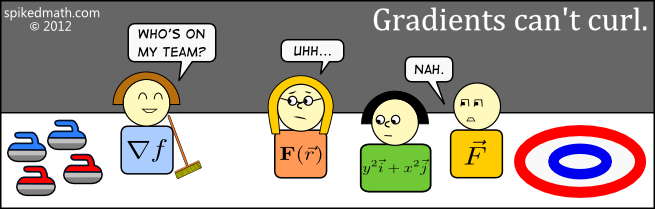
\includegraphics[width=10cm]{501-curling-with-gradients.png}
        \else
            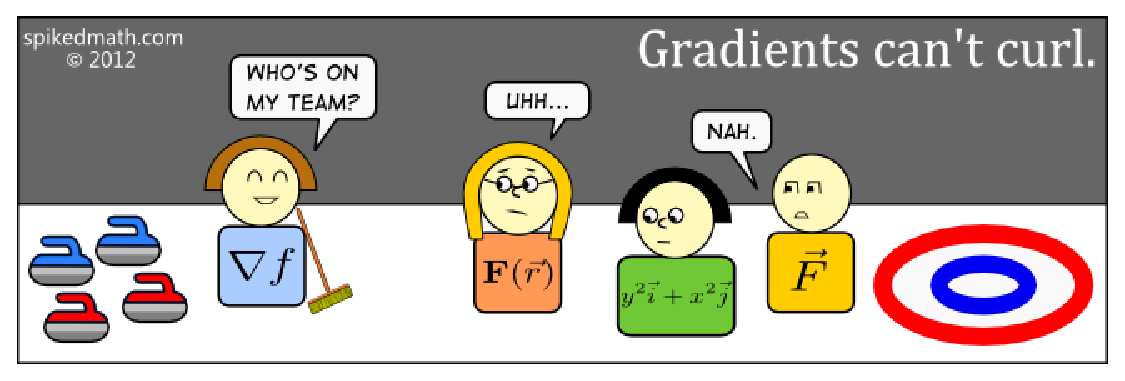
\includegraphics[width=10cm]{501-curling-with-gradients.eps}
        \fi

        {\tiny De \href{http://spikedmath.com/501.html}{Spiked math}, publié sous \href{http://creativecommons.org/licenses/by-nc-sa/2.5/ca/}{licence Creative Commons}.}
\end{center}


%+++++++++++++++++++++++++++++++++++++++++++++++++++++++++++++++++++++++++++++++++++++++++++++++++++++++++++++++++++++++++++
\section[Interprétation de la divergence]{Interprétation géométrique et physique de la divergence}
%+++++++++++++++++++++++++++++++++++++++++++++++++++++++++++++++++++++++++++++++++++++++++++++++++++++++++++++++++++++++++++


En physique, on dit qu'un champ de vecteurs à divergence nulle est \defe{incompressible}{incompressible!champ de vecteur}. Nous allons essayer de comprendre pourquoi. Lorsqu'un fluide incompressible se déplace, il faut qu'en chaque point il y autant de fluide qui rentre que de fluide qui sort. Nous allons voir sur quelques exemples que la divergence d'un champ de vecteurs est le «bilan de masse» d'un fluide qui se déplace selon le champ de vecteurs.

Si en un point la divergence est positive, cela signifie qu'il y a une perte de masse et si la divergence est négative, cela signifie qu'il y a une accumulation de masse.

Prenons par exemple un fluide qui se déplace selon le champ de vitesse montré à figure \ref{LabelFigDivergenceUn}.
\newcommand{\CaptionFigDivergenceUn}{Le champ de vecteurs $F(x,y)=\frac{1}{ x }(1,0)$.}
\input{Fig_DivergenceUn.pstricks}

Étant donné que la vitesse diminue lorsque $x$ avance, il y a une accumulation de fluide. Regardez en effet la quantité de fluide qui rentre dans le rectangle par rapport à la quantité de fluide qui en sort. Ce champ de vecteurs a pour équation :
\begin{equation}
    F(x,y)=\frac{1}{ x }\begin{pmatrix}
        1    \\ 
        0    
    \end{pmatrix}=\begin{pmatrix}
        1/x    \\ 
        0    
    \end{pmatrix}.
\end{equation}
Sa divergence vaut donc
\begin{equation}
    (\nabla\cdot F)(x,y)=\frac{ \partial F_x }{ \partial x }(x,y)+\underbrace{\frac{ \partial F_y }{ \partial y }(x,y)}_{=0}=-\frac{1}{ x^2 }.
\end{equation}
Cette divergence étant négative, il y a bien accumulation de fluide en tout point, et d'autant plus que $x$ est petit.

\begin{example}     \label{ExamDivFrotOM}

    Prenons le champ de vecteurs tournant
    \begin{equation}
        F(x,y)=\frac{1}{ \sqrt{x^2+y^2} }\begin{pmatrix}
            y    \\ 
            -x    
        \end{pmatrix}
    \end{equation}
    représenté à la figure \ref{LabelFigDivergenceDeux}. Cela est un vecteur qui est constamment perpendiculaire au rayon.

    \newcommand{\CaptionFigDivergenceDeux}{Le champ de vecteurs $F(x,y)=(y,-x)$.}
    \input{Fig_DivergenceDeux.pstricks}

    Un fluide dont la vitesse serait donné par ce champ de vecteur se contente de tourner. Intuitivement il ne devrait pas y avoir de divergence parce qu'il n'y a aucune accumulation de fluide. En effet,
    \begin{equation}
        \nabla\cdot F(x,y)=\frac{ -2xy }{ (x^2+y^2)^2 }+\frac{ 2xy }{ (x^2+y^2)^2 }=0.
    \end{equation}
\end{example}

\begin{example}
    Prenons le cas du champ de force de gravitation :
    \begin{equation}
        F(x,y,z)=\frac{1}{ (x^2+y^2+z^2)^{3/2} }\begin{pmatrix}
            x    \\ 
            y   \\
            z
        \end{pmatrix}.
    \end{equation}
    Nous pouvons rapidement remarquer que $\nabla\cdot F=0$. Est-ce que cela peut se comprendre sur le dessin de la figure \ref{LabelFigDivergenceTrois} ?
    \newcommand{\CaptionFigDivergenceTrois}{Le champ de vecteur de la gravité. Nous avons tracé, sur les deux cercles la même densité de vecteurs, c'est à dire le même nombre de vecteurs par unité de surface.}
    \input{Fig_DivergenceTrois.pstricks}

    Essayons de voir combien de fluide entre dans la zone bleue et combien en sort. D'abord, il est certain que les vecteurs qui sortent sont plus courts que ceux qui rentrent, ce qui voudrait dire qu'il y a plus de fluide qui rentre. Mais on voit également que le \emph{nombre} de vecteurs qui sortent est plus grand parce que la seconde sphère est plus grande et qu'il y a un vecteur en chaque point de la sphère.

    Intuitivement nous pouvons dire que la quantité qui rentre dans la sphère de rayon $r_1$ donnée par la taille des vecteurs entrants multiplié par la surface de la sphère, c'est à dire
    \begin{equation}        \label{EqQpinormeVectoOM}
        4\pi r_1^2\| F(x,y,z) \|,
    \end{equation}
    mais $\| F(x,y,z) \|=\frac{1}{ r_1^2 }$, donc la quantité de fluide entrant est $4\pi$. La quantité de fluide sortant sera la même.

    Cela explique deux choses
    \begin{enumerate}
        \item
            Pourquoi les forces de gravitation et électromagnétiques sont en $1/r^2$; c'est parce que nous vivons dans un monde avec trois dimensions d'espace. En étudiant très précisément le champ de gravitation, certains physiciens espèrent trouver des déviations expérimentales par rapport à la règle du \( 1/r^2\); cela \emph{pourrait} être un signe que l'espace contient des dimensions supplémentaires.
        \item
            Pourquoi il y a un $4\pi$ comme coefficient dans beaucoup d'équations en électromagnétisme; en particulier dans certaines anciennes unités de flux.
    \end{enumerate}
    
\end{example}

\begin{remark}
    Nous allons voir plus loin comment s'assurer que l'équation \eqref{EqQpinormeVectoOM} représente bien la «quantité de fluide» qui rentre dans la zone délimitée
\end{remark}


%+++++++++++++++++++++++++++++++++++++++++++++++++++++++++++++++++++++++++++++++++++++++++++++++++++++++++++++++++++++++++++
\section{Quelques formules de Leibnitz}
%+++++++++++++++++++++++++++++++++++++++++++++++++++++++++++++++++++++++++++++++++++++++++++++++++++++++++++++++++++++++++++

La divergence étant une combinaison de dérivées, il n'est pas tellement étonnant que la divergence de produits donne lieux à des formules en deux termes. Si $f$ est une fonction et si $F$ et $G$ sont des champs de vecteurs, nous avons (sans démonstrations) :
\begin{equation}        \label{EqLeinDivNablRotOM}
    \begin{aligned}[]
        \nabla\cdot(fF)&=f\nabla\cdot F+F\cdot\nabla f\\
        \nabla\cdot(F\times G)&=G\cdot\nabla\times F-F\cdot\nabla\times G.
    \end{aligned}
\end{equation}
Nous avons aussi, pour le rotationnel,
\begin{equation}        \label{EqLeinRotfFFOM}
    \nabla\times(fF)=f\nabla\times F+\nabla f\times F.
\end{equation}


\chapter{Coordonnées curvilignes orthogonales}
% This is part of Mes notes de mathématique
% Copyright (c) 2011-2012,2015
%   Laurent Claessens
% See the file fdl-1.3.txt for copying conditions.

%+++++++++++++++++++++++++++++++++++++++++++++++++++++++++++++++++++++++++++++++++++++++++++++++++++++++++++++++++++++++++++
\section{La différentielle revisitée}
%+++++++++++++++++++++++++++++++++++++++++++++++++++++++++++++++++++++++++++++++++++++++++++++++++++++++++++++++++++++++++++

%---------------------------------------------------------------------------------------------------------------------------
\subsection{Les formes différentielles de base}
%---------------------------------------------------------------------------------------------------------------------------

Si la fonction $f\colon \eR^n\to \eR$ est différentiable alors la différentielle en $a\in\eR^n$ est l'application
\begin{equation}        \label{EqFormDiffdfahOM}
    \begin{aligned}
        df_a\colon \eR^n&\to \eR \\
        u&\mapsto \frac{ \partial f }{ \partial x_1 }(a)u_1+\cdots+\frac{ \partial f }{ \partial x_n }(a)u_n.
    \end{aligned}
\end{equation}
Considérons en particulier la fonction qui à $x\in\eR^n$ fait correspondre $x_i\in\eR$. Par abus de notations,  nous la noterons $x_i$. Nous avons 
\begin{equation}
    \frac{ \partial x_i }{ \partial x_j }=\delta_{ij}.
\end{equation}
Par exemple $\partial_yx=0$ et $\partial_xx=1$. Toutes les dérivées partielles de $x_i$ s'annulent sauf la $i$ème qui vaut $1$. Par conséquent
\begin{equation}
    \begin{aligned}
        dx_i\colon \eR^n&\to \eR \\
        u&\mapsto u_i. 
    \end{aligned}
\end{equation}

\begin{remark}
    En toute rigueur nous devrions écrire $(dx_i)_a$. Mais étant donné que
    \begin{equation}
        (dx_i)_a(u)=(dx_i)_b(u)
    \end{equation}
    pour tout points $a$, $b$ et pour tout vecteurs $u$, nous nous permettons de simplifier la notation en ne précisant pas en quel point nous calculons la différentielle de $x_i$.
\end{remark}

Étant donné que $dx_i(u)=u_i$, nous pouvons récrire la formule \eqref{EqFormDiffdfahOM} en remplaçant $u_i$ par $dx_i(u)$ :
\begin{equation}
    df_a(u)=\frac{ \partial f }{ \partial x_1 }(a)dx_1(u)+\cdots+\frac{ \partial f }{ \partial x_n }(a)dx_n(u).
\end{equation}
En tant que application linéaire, $df_a$ est une combinaison linéaire des $dx_i$. En notations compacte :
\begin{equation}
    df_a=\sum_{i=1}^n\frac{ \partial f }{ \partial x_i }(a)dx_i.
\end{equation}

%---------------------------------------------------------------------------------------------------------------------------
\subsection{Différentielles de fonctions composées}
%---------------------------------------------------------------------------------------------------------------------------

Cette façon de voir la différentielle nous permet de jeter un nouveau regard sur la formule de différentiation des fonctions composées. Soient
\begin{equation}
    \begin{aligned}[]
        f\colon \eR^p&\to \eR^n\\
        g\colon \eR^n&\to \eR,
    \end{aligned}
\end{equation}
et $h\colon \eR^p\to \eR$ définie par 
\begin{equation}
    h(u)=h\big( f(u) \big)=(g\circ f)(u).
\end{equation}
Nous allons noter $x$ les coordonnées de $\eR^p$, $a$ un point de $\eR^p$ et $u$, un vecteur de $\eR^p$ accroché au point $a$. Pour $\eR^n$, les notations seront que les coordonnées sont $y$, $b$ est un point de $\eR^n$ et $v$ est un vecteur «accroché» au point $b$.

Nous avons
\begin{equation}
    dg_b(v)=\sum_{i=1}^n\frac{ \partial g }{ \partial y_i }(b)dy_i(v).
\end{equation}
Ici $dy_i(v)$ signifie la $i$ème composante de $v$. C'est simplement $v_i$. Cette formule étant valable pour tout point $b\in\eR^n$ et pour tout vecteur $v$, nous pouvons l'écrire en particulier pour
\begin{subequations}
    \begin{numcases}{}
        b=f(a)\\
        v=df_a(u).
    \end{numcases}
\end{subequations}
Cela donne
\begin{equation}        \label{EqdgfadfauOM}
    dg_{f(a)}\big( df_a(u) \big)=\sum_{i=1}^n\frac{ \partial g }{ \partial y_i }\big( f(a) \big)dy_i\big( df_a(u) \big).
\end{equation}
Mais 
\begin{equation}
    df_a(u)=\sum_{j=1}^p\frac{ \partial f }{ \partial x_j }(a)dx_j(u),
\end{equation}
donc la $i$ème composante de ce vecteur est
\begin{equation}
     \big( df_a(u)\big)_i=\sum_{j=1}^p\frac{ \partial f_i }{ \partial x_j }(a)dx_j(u).
\end{equation}
En remplaçant $dy_i\big( df_a(u) \big)$ par cela dans l'expression \eqref{EqdgfadfauOM}, nous trouvons
\begin{equation}
    dg_{f(a)}\big( df_a(u) \big)=\sum_{i=1}^n\frac{ \partial g }{ \partial y_i }\big( f(a) \big)\sum_{j=1}^p\frac{ \partial f_i }{ \partial x_j }(a)dx_j(u).
\end{equation}
Nous pouvons vérifier que cela est la différentielle de $g\circ f$ au point $a$ appliquée au vecteur $u$. En effet
\begin{equation}
    d(g\circ f)_a(u)=\sum_{j=1}^p\frac{ \partial (g\circ f) }{ \partial x_j }(a)dx_j(u),
\end{equation}
tandis que, par la dérivation de fonctions composées, 
\begin{equation}        \label{EqDerCompofgOM}
    \frac{ \partial (g\circ f) }{ \partial x_j }(a)=\sum_{i=1}^n\frac{ \partial g }{ \partial y_i }\big( f(a) \big)\frac{ \partial f_i }{ \partial x_j }(a).
\end{equation}
Au final, ce que nous avons prouvé est que
\begin{equation}
    d(g\circ f)_a(u)=dg_{f(a)}\big( df_a(u) \big).
\end{equation}

%---------------------------------------------------------------------------------------------------------------------------
\subsection{Passage aux coordonnées polaires}
%---------------------------------------------------------------------------------------------------------------------------

Le changement de coordonnées pour les polaires est la fonction
\begin{equation}
    f\begin{pmatrix}
        r    \\ 
        \theta    
    \end{pmatrix}=\begin{pmatrix}
        x    \\ 
        y    
    \end{pmatrix}=\begin{pmatrix}
        r\cos\theta    \\ 
        r\sin\theta    
    \end{pmatrix}.
\end{equation}
Considérons une fonction $g$ sur $\eR^2$, et définissons la fonction $\tilde g$ par
\begin{equation}
    \tilde g(r,\theta)=g(r\cos\theta,r\sin\theta).
\end{equation}
La formule \eqref{EqDerCompofgOM} permet de trouver les dérivées partielles de $g$ par rapport à $r$ et $\theta$ en termes de celles par rapport à $x$ et $y$ de $g$.

Pour faire le lien avec les notations du point précédent, nous avons
\begin{equation}
    \begin{aligned}[]
        f_1(r,\theta)&=r\cos(\theta)\\
        f_2(r,\theta)&=r\sin(\theta)\\
        (x_1,x_2)&\to(r,\theta)\\
        (y_1,y_2)&\to(x,y).
    \end{aligned}
\end{equation}
Nous avons donc 
\begin{equation}
    \begin{aligned}[]
        \frac{ \partial \tilde g }{ \partial r }(r,\theta)&=\sum_{i=1}^2\frac{ \partial g }{ \partial x_i }\big( f(r,\theta) \big)\frac{ \partial f_i }{ \partial r }(r,\theta)\\
        &=\frac{ \partial g }{ \partial x }(r\cos\theta,r\sin\theta)\frac{ \partial \big( r\cos\theta \big) }{ \partial r }(r,\theta)\\
        &\quad+\frac{ \partial g }{ \partial y }(r\cos\theta,r\sin\theta)\frac{ \partial \big( r\sin\theta\big) }{ \partial r }(r,\theta)\\
        &=\cos\theta\frac{ \partial g }{ \partial x }(r\cos\theta,r\sin\theta)+\sin\theta\frac{ \partial g }{ \partial y }(r\cos\theta,r\sin\theta).
    \end{aligned}
\end{equation}

Prenons par exemple $g(x,y)=\frac{1}{ x^2+y^2 }$. Étant donné que
\begin{equation}
    \frac{ \partial g }{ \partial x }=\frac{ -2x }{ (x^2+y^2)^2 },
\end{equation}
nous avons
\begin{equation}
    \frac{ \partial g }{ \partial x }(r\cos\theta,r\sin\theta)=\frac{ -2\cos\theta }{ r^3 }.
\end{equation}
En utilisant la formule,
\begin{equation}
    \frac{ \partial \tilde g }{ \partial r }(r,\theta)=\cos(\theta)\left( \frac{ -2\cos\theta }{ r^3 } \right)+\sin(\theta)\left( \frac{ -2\sin\theta }{ r^3 } \right)=-\frac{ 2 }{ r^3 }.
\end{equation}
Nous pouvons vérifier directement que cela est correct. En effet
\begin{equation}
    \tilde g(r,\theta)=g(r\cos\theta,r\sin\theta)=\frac{1}{ r^2 },
\end{equation}
dont la dérivée par rapport à $r$ vaut $-2/r^3$.

En ce qui concerne la dérivée par rapport à $\theta$, nous avons
\begin{equation}
    \begin{aligned}[]
    \frac{ \partial \tilde g }{ \partial \theta }&=\frac{ \partial g }{ \partial x }(r\cos\theta,r\sin\theta)\frac{ \partial \big( r\cos(\theta) \big) }{ \partial \theta }+\frac{ \partial g }{ \partial y }(r\cos\theta,r\sin\theta)\frac{ \partial \big( r\sin(\theta) \big) }{ \partial \theta }\\
    &=\left( \frac{ -2\cos\theta }{ r^3 } \right)(-r\sin\theta)+\left( \frac{ -2\sin\theta }{ r^3 } \right)(r\cos\theta)\\
    &=0.
    \end{aligned}
\end{equation}

En résumé et avec quelques abus de notations :
\begin{equation}
    \begin{aligned}[]
        \frac{ \partial \tilde g }{ \partial r }&=\cos(\theta)\frac{ \partial g }{ \partial x }+\sin(\theta)\frac{ \partial g }{ \partial y }\\
        \frac{ \partial \tilde g }{ \partial \theta }&=-r\sin(\theta)\frac{ \partial g }{ \partial x }+r\cos(\theta)\frac{ \partial g }{ \partial y }\\
    \end{aligned}
\end{equation}

%+++++++++++++++++++++++++++++++++++++++++++++++++++++++++++++++++++++++++++++++++++++++++++++++++++++++++++++++++++++++++++
\section{Théorie générale}
%+++++++++++++++++++++++++++++++++++++++++++++++++++++++++++++++++++++++++++++++++++++++++++++++++++++++++++++++++++++++++++

%---------------------------------------------------------------------------------------------------------------------------
\subsection{Base locale}
%---------------------------------------------------------------------------------------------------------------------------

Les coordonnées sphériques et cylindriques sont deux systèmes de coordonnées «un peu courbe» qui existent sur $\eR^3$. Il en existe de nombreux autres, que nous appelons \defe{coordonnées curvilignes}{coordonnées!curvilignes}. Des coordonnées curvilignes sur $\eR^3$ est n'importe quel\footnote{Nous n'entrons pas dans les détails de régularité.} système qui permet de repérer un point de $\eR^3$ à partir de trois nombres.

Il s'agit donc d'un ensemble de trois applications 
\begin{equation}
    x_i\colon \eR^3\to \eR.
\end{equation}
Les coordonnées cylindriques sont
\begin{subequations}
    \begin{numcases}{}
        x_1(r,\theta,z)=r\cos\theta\\
        x_2(r,\theta,z)=r\sin\theta\\
        x_3(r,\theta,z)=z
    \end{numcases}
\end{subequations}

Soit donc un système général $q=(q_1,q_2,q_3)$ et 
\begin{equation}
    M(q)=\begin{pmatrix}
        x_1(q)    \\ 
        x_2(q)    \\ 
        x_3(q)    
    \end{pmatrix}.
\end{equation}
Si nous fixons $q_2$ et $q_3$ et que nous laissons varier $q_1$, nous obtenons une courbe\footnote{Dans le cas des sphériques, c'est une demi-droite horizontale d'angle $q_2$ et de hauteur $q_3$.} dont nous pouvons considérer le vecteur vitesse, c'est à dire le vecteur tangent. En chaque point nous avons ainsi trois vecteurs
\begin{equation}
    \frac{ \partial M }{ \partial q_i }(q).
\end{equation}
Nous disons que le système de coordonnées curviligne est \defe{orthogonal}{orthogonal!coordonnées curviligne} si ces trois vecteurs sont orthogonaux. Dans la suite nous supposerons que c'est toujours le cas.

Nous posons
\begin{equation}
    h_i=\left\| \frac{ \partial M }{ \partial q_i } \right\|
\end{equation}
et nous considérons les trois vecteurs normés
\begin{equation}        \label{EqDefeihMqOM}
    e_i=h_i^{-1}\frac{ \partial M }{ \partial q_i }.
\end{equation}
Les trois vecteurs $\{ e_1,e_2,e_3 \}$ forment une base orthonormée dite \defe{base locale}{base!locale}. Ce sont des vecteurs liés\footnote{En géométrie différentielle on dira que ce sont des élément de l'espace tangent, mais c'est une toute autre histoire.} au point $M$.

%---------------------------------------------------------------------------------------------------------------------------
\subsection{Importance de l'orthogonalité}
%---------------------------------------------------------------------------------------------------------------------------

Nous avons dit que nous nous restreignons au cas où les vecteurs $e_i$ sont orthogonaux. En termes de produits scalaires, cela signifie
\begin{equation}
    e_i\cdot e_j=\delta_{ij}.
\end{equation}
Nous en étudions maintenant quelque conséquence. L'équation \eqref{EqDefeihMqOM} peut s'écrire plus explicitement sous la forme
\begin{equation}
    e_i=\sum_k h_i^{-1}\frac{ \partial x_k }{ \partial q_i }1_k.
\end{equation}
Notez que pour chaque $k$ et $i$, la quantité $h_i^{-1}\frac{ \partial x_k }{ \partial q_i }$ est un simple nombre. Nous allons les mettre dans une matrice :
\begin{equation}
    A_{ki}=h_i^{-1}\frac{ \partial x_k }{ \partial q_i }.
\end{equation}
Cela nous donne le changement de base
\begin{equation}        \label{EqChmBaseeisAkiAkOM}
    e_i=\sum_kA_{ki}1_k.
\end{equation}
Le produit $e_i\cdot e_j$ s'écrit alors
\begin{equation}
    \begin{aligned}[]
        e_i\cdot e_j&=\sum_{kl}A_{ki}A_{lj}\underbrace{1_k\cdot 1_l}_{=\delta_{kl}}\\
        &=\sum_{kl}A_{ki}A_{lj}\delta_{kl}\\
        &=\sum_kA_{ki}A_{kj}\\
        &=\sum_k(A^T)_{ik}A_{kj}.
    \end{aligned}
\end{equation}
Or cela doit valoir $\delta_{ij}$. Par conséquent 
\begin{equation}
    A^T=A^{-1}.
\end{equation}
Le fait que les coordonnées curvilignes considérées soient orthogonales s'exprime donc par la fait que la matrice de changement de base est une matrice orthogonale.

Cette circonstance nous permet d'inverser le changement de base \eqref{EqChmBaseeisAkiAkOM} en multipliant cette équation par $(A^{-1})_{il}$ des deux côtés et en faisant la somme sur $i$ :
\begin{equation}
    \sum_i (A^{-1})_{il}e_i=\sum_{kl}\underbrace{A_{ki}(A^{-1})_{il}}_{=\delta_{kl}}1_k,
\end{equation}
par conséquent
\begin{equation}
    \sum_i(A^T)_{il}e_i=1_l,    
\end{equation}
et
\begin{equation}        \label{EqChamvarunlAeiOM}
    1_l=\sum_iA_{li}e_i=\sum_ih_i^{-1}\frac{ \partial x_l }{ \partial q_i }e_i.
\end{equation}
Armés de cette importante formule, nous pouvons exprimer les quantités que nous connaissons dans la base canonique en termes de la base locale.

Une autre conséquence du fait que $e_1$, $e_2$ et $e_3$ est une base orthonormée est que, éventuellement en réordonnant les vecteurs, on a
\begin{equation}
    \begin{aligned}[]
        e_1\times e_2&=e_3\\
        e_2\times e_3&=e_1\\
        e_3\times e_1&=e_2
    \end{aligned}
\end{equation}
Ces trois relations s'écrivent en une seule avec
\begin{equation}
    e_i\times e_j=\sum_{k}\epsilon_{ijk}e_k
\end{equation}
où 
\begin{equation}
    \epsilon_{ijk}=\begin{cases}
        0    &   \text{si} i,j,k \text{ne sont pas tous différents}\\
        1    &    \text{si } ijk \text{ se ramène à 123 par un nombre pair de permutations}\\
        -1    &    \text{si }ijk \text{ se ramène à 123 par un nombre impair de permutations}
    \end{cases}
\end{equation}
est le \defe{symbole de Levi-Civita}{Levi-Civita}. La formule du produit vectoriel peut également être utilisée à l'envers sous la forme
\begin{equation}        \label{EqekeitimesejOM}
    e_k=\frac{ 1 }{2}\sum_{ij}\epsilon_{ijk}\,e_i\times e_j.
\end{equation}

Le symbole de Levi-Civita possède de nombreuses formules. En voici certaines, facilement démontrables en considérant tous les cas :
\begin{equation}
    \epsilon_{ijk}\epsilon_{ijl}=\delta_{kl}| \epsilon_{ijk} |.
\end{equation}
Grâce au symboles de Levi-Civita, le produit mixte des vecteurs de base a une belle forme :
\begin{equation}        \label{EqProdMixteepsilonCicivrOM}
    e_l\cdot(e_i\times e_j)=\sum_k\epsilon_{ijk}e_l\times e_k=\sum_k\epsilon_{ijk}\delta_{lk}=\epsilon_{ijl}.
\end{equation}

%+++++++++++++++++++++++++++++++++++++++++++++++++++++++++++++++++++++++++++++++++++++++++++++++++++++++++++++++++++++++++++
\section{Gradient en coordonnées curvilignes}
%+++++++++++++++++++++++++++++++++++++++++++++++++++++++++++++++++++++++++++++++++++++++++++++++++++++++++++++++++++++++++++

Soit $(x,y,z)\mapsto f(x,y,z)$ une fonction sur $\eR^3$. Nous pouvons la composer avec les coordonnées curvilignes $q$ pour obtenir la fonction
\begin{equation}
    \tilde f(q_1,q_2,q_3)=f\big( x_1(q),x_2(x),x_3(q) \big).
\end{equation}
Nous disons que $\tilde f$ est l'expression de $f$ dans les coordonnées $q$. Nous savons déjà comment calculer le gradient de $f$ en coordonnées cartésiennes :
\begin{equation}
    F(x,y, z)=\nabla f(x,y,z)=\begin{pmatrix}
        \partial_xf(x,y,z)    \\ 
        \partial_yf(x,y,z)    \\ 
        \partial_zf(x,y,z)    \
    \end{pmatrix}.
\end{equation}
Cela est un vecteur lié au point $(x,y,z)$. Nous voudrions exprimer ce vecteur dans la base $\{ e_1,e_2,e_3 \}$. En d'autres termes, nous voudrions trouver les nombres $\tilde F_1$, $\tilde F_2$ et $\tilde F_3$ tels que
\begin{equation}
    F(x,y,z)=F\big( x(q),y(q),z(q) \big)=\tilde F_1e_1+\tilde F_2e_2+\tilde F_3e_3.
\end{equation}
Ces nombres seront des fonctions de $(q_1,q_2,q_3)$.

Par définition,
\begin{equation}
    \nabla f=\sum_l\frac{ \partial f }{ \partial x_l }1_l.
\end{equation}
En remplaçant $1_l$ par sa valeur en termes des $e_i$ par la formule \eqref{EqChamvarunlAeiOM},
\begin{equation}
    \begin{aligned}[]
        \nabla f&=\sum_l\frac{ \partial f }{ \partial x_l }1_l\\
        &=\sum_l\frac{ \partial f }{ \partial x_l }\sum_ih_i^{-1}\frac{ \partial x_l }{ \partial q_i }e_i\\
        &=\sum_{il}\frac{1}{ h_i }\frac{ \partial f }{ \partial x_l }\frac{ \partial x_l }{ \partial q_i }e_i\\
        &=\sum_i\frac{1}{ h_i }\frac{ \partial \tilde f }{ \partial q_i }e_i.
    \end{aligned}
\end{equation}

Plus explicitement,
\begin{equation}        \label{EqGradientenCurviligneOM}
    \nabla f\big( x(q),y(q),z(q) \big)=\sum_i \frac{1}{ h_i(q) }\frac{ \partial \tilde f }{ \partial q_i }(q)e_i
\end{equation}
où
\begin{equation}
    h_i(q)=\left\| \frac{ \partial M }{ \partial q_i }(q) \right\|.
\end{equation}
Le plus souvent nous n'allons pas noter explicitement la dépendance de $h_i$ en $q$.

Quelques formulaires intéressants sont en appendice de \cite{Schomblond_em}.

%---------------------------------------------------------------------------------------------------------------------------
\subsection{Coordonnées polaires}
%---------------------------------------------------------------------------------------------------------------------------

Les coordonnées curvilignes polaires sont données par
\begin{equation}
    M(r,\theta)=\begin{pmatrix}
        r\cos(\theta)    \\ 
        r\sin(\theta)    
    \end{pmatrix},
\end{equation}
et par conséquent
\begin{equation}
    \begin{aligned}[]
        \frac{ \partial M }{ \partial r }&=\begin{pmatrix}
            \cos(\theta)    \\ 
            \sin(\theta)    
        \end{pmatrix},&\frac{ \partial M }{ \partial \theta }=\begin{pmatrix}
            -r\sin(\theta)    \\ 
            r\cos(\theta)    
        \end{pmatrix}.
    \end{aligned}
\end{equation}
Nous avons les normes $h_r=1$ et $h_{\theta}=r$, et donc les vecteurs de la base locale en $(r,\theta)$ sont
\begin{equation}
    e_r=\begin{pmatrix}
        \cos(\theta)    \\ 
        \sin(\theta)    
    \end{pmatrix}=\cos(\theta)e_x+\sin(\theta)e_y
\end{equation}
ainsi que
\begin{equation}
    e_{\theta}=\begin{pmatrix}
        -\sin(\theta)    \\ 
        \cos(\theta)    
    \end{pmatrix}=-\sin(\theta)e_x+\cos(\theta)e_y.
\end{equation}


Ces vecteurs sont représentés à la figure \ref{LabelFigCurvilignesPolaires}. Notez qu'il y en a une paire différente en chaque point.
\newcommand{\CaptionFigCurvilignesPolaires}{En brun, les lignes que le point suivrait si on ne variait qu'une coordonnées polaire à la fois. Les vecteurs rouges sont les vecteurs $e_{r}$ et $e_{\theta}$.}
\input{pictures_tex/Fig_CurvilignesPolaires.pstricks}


%---------------------------------------------------------------------------------------------------------------------------
\subsection{Coordonnées cylindriques}
%---------------------------------------------------------------------------------------------------------------------------

Les coordonnées cylindriques sont les mêmes que les coordonnées polaires à part qu'il faut écrire
\begin{equation}
    M(r,\theta,z)=\begin{pmatrix}
        r\cos(\theta)    \\ 
        r\sin(\theta)    \\ 
        z    
    \end{pmatrix},
\end{equation}
et nous avons le vecteur de base supplémentaire
\begin{equation}
    e_z=\frac{ \partial M }{ \partial z }=\begin{pmatrix}
        0    \\ 
        0    \\ 
        1    
    \end{pmatrix}
\end{equation}
parce que $h_z=1$.

%---------------------------------------------------------------------------------------------------------------------------
\subsection{Coordonnées sphériques}
%---------------------------------------------------------------------------------------------------------------------------

Les coordonnées curvilignes sphériques sont données par
\begin{equation}
    M(\rho,\theta,\varphi)=
    \begin{pmatrix}
        \rho\sin(\theta)\cos(\varphi)    \\ 
        \rho\sin(\theta)\sin(\varphi)    \\ 
        \rho\cos(\theta)
    \end{pmatrix},
\end{equation}
dont les dérivées sont données par
\begin{equation}
    \begin{aligned}[]
        \frac{ \partial M }{ \partial r }&=\begin{pmatrix}
        \sin(\theta)\cos(\varphi)    \\ 
        \sin(\theta)\sin(\varphi)    \\ 
        \cos(\theta)
    \end{pmatrix},
    &\frac{ \partial M }{ \partial \theta }&=
    \begin{pmatrix}
        \rho\cos(\theta)\cos(\varphi)    \\ 
        \rho\cos(\theta)\sin(\varphi)    \\ 
        -\rho\sin(\theta)
    \end{pmatrix},\\
    \frac{ \partial M }{ \partial \varphi }&=
    \begin{pmatrix}
        -\rho\sin(\theta)\sin(\varphi)    \\ 
        \rho\sin(\theta)\cos(\varphi)    \\ 
        0
    \end{pmatrix}
    \end{aligned}
\end{equation}
Les normes de ces vecteurs sont $h_{\rho}=1$, $h_{\theta}=\rho$ et $h_{\varphi}=\rho\sin(\theta)$. Les vecteurs de la base locale en $(\rho,\theta,\varphi)$ sont donc
\begin{equation}
    \begin{aligned}[]
        e_r&=\begin{pmatrix}
        \sin(\theta)\cos(\varphi)    \\ 
        \sin(\theta)\sin(\varphi)    \\ 
        \cos(\theta)
    \end{pmatrix},
    &e_{\theta}&=
    \begin{pmatrix}
        \cos(\theta)\cos(\varphi)    \\ 
        \cos(\theta)\sin(\varphi)    \\ 
        -\sin(\theta)
    \end{pmatrix},\\
    e_{\varphi}&=
    \begin{pmatrix}
        -\sin(\varphi)    \\ 
        \cos(\varphi)    \\ 
        0
    \end{pmatrix}
    \end{aligned}
\end{equation}

Nous pouvons exprimer le gradient d'une fonction en coordonnées sphériques en utilisant la formule \eqref{EqGradientenCurviligneOM} :
\begin{equation}        \label{EqGradientSpheriqueOM}
    \nabla\tilde f(\rho,\theta,\varphi)=\frac{ \partial \tilde f }{ \partial \rho }e_{\rho}+\frac{1}{ \rho }\frac{ \partial \tilde f }{ \partial \theta }e_{\theta}+\frac{1}{ \rho\sin(\theta) }\frac{ \partial \tilde f }{ \partial \varphi }r_{\varphi}.
\end{equation}
Cette expression peut paraître peu pratique parce que les vecteurs $e_{\rho}$, $e_{\theta}$ et $e_{\varphi}$ eux-mêmes changent en chaque point. Elle est effectivement peu adaptée au dessin, mais elle est très pratique pour des fonctions ayant des symétries.

\begin{example}
    Le potentiel de la gravitation est la fonction
    \begin{equation}
        V(x,y,z)=\frac{1}{ \sqrt{x^2+y^2+z^2} }.
    \end{equation}
    En coordonnées sphériques elle s'écrit
    \begin{equation}
        \tilde V(\rho,\theta,\varphi)=\frac{1}{ \rho }.
    \end{equation}
    En voila une fonction qu'elle est facile à dériver, contrairement à $V$ ! En suivant la formule \eqref{EqGradientSpheriqueOM}, nous avons immédiatement
    \begin{equation}
        \nabla\tilde V=-\frac{1}{ \rho^2 }e_{\rho}.
    \end{equation}
    Nous voyons immédiatement que cela est un champ de vecteurs dont la norme diminue comme le carré de la distance à l'origine et qui est en permanence dirigé vers l'origine.
\end{example}


%+++++++++++++++++++++++++++++++++++++++++++++++++++++++++++++++++++++++++++++++++++++++++++++++++++++++++++++++++++++++++++
\section{Divergence en coordonnées curvilignes}
%+++++++++++++++++++++++++++++++++++++++++++++++++++++++++++++++++++++++++++++++++++++++++++++++++++++++++++++++++++++++++++

Nous savons que 
\begin{equation}
    \nabla\tilde f=\sum_j\frac{1}{ h_j }\frac{ \partial \tilde f }{ \partial q_j }e_j.
\end{equation}
Nous pouvons en particulier considérer la fonction $f(q)=q_i$. De la même manière que nous avions noté $x_i$ la fonction $x\mapsto x_i$, nous notons $q_i$ la fonction $q\mapsto q_i$. Le gradient de cette fonction est donné par
\begin{equation}
    \nabla q_i=\sum_j\frac{1}{ h_j }\frac{ \partial q_i }{ \partial q_j }e_j,
\end{equation}
mais $\frac{ \partial q_i }{ \partial q_j }=\delta_{ij}$, donc
\begin{equation}
    \nabla q_i=\frac{ e_i }{ h_i },
\end{equation}
ou encore
\begin{equation}
    e_i=h_i\nabla q_i.
\end{equation}
Cela n'est pas étonnant : la direction dans laquelle la coordonnées $q_i$ varie le plus est le vecteur $e_i$ qui donne la tangente à la courbe obtenue lorsque \emph{seul} $q_i$ varie.

Commençons par calculer la divergence de $e_i$. En utilisant la formule \eqref{EqekeitimesejOM},
\begin{equation}
    \nabla\cdot e_k=\frac{ 1 }{2}\sum_{ij}\epsilon_{ijk}\,\nabla\cdot (e_i\times e_j).
\end{equation}
Nous avons, en utilisant les règles de Leibnitz \eqref{EqLeinDivNablRotOM}, 
\begin{equation}
    \begin{aligned}[]
        \nabla\cdot(e_i\times e_j)&=\nabla\cdot(h_i\nabla q_i\times h_j\nabla q_j)\\
        &=\nabla(h_ih_j)\cdot\big( \nabla q_i\times\nabla q_j \big)+h_ih_j\nabla\cdot\big( \nabla q_i\times\nabla q_j \big)\\
        &=\nabla(h_ih_j)\cdot\big( \nabla q_i\times\nabla q_j \big)\\
        &\quad+h_ih_j\nabla q_j\cdot\big( \underbrace{\nabla\times\nabla q_i}_{=0} \big)\\
        &\quad+h_ih_j\nabla q_i\cdot\big( \underbrace{\nabla\times\nabla q_j}_{=0} \big)
    \end{aligned}
\end{equation}
Cela nous fait
\begin{equation}
    \nabla\cdot e_k=\sum_{ij}\epsilon_{ijk}\frac{ \nabla(h_ih_j) }{ h_ih_j }\cdot (e_i\times e_j).
\end{equation}
parce que $\nabla q_i=h_i^{-1}e_i$. Nous pouvons développer le gradient qui intervient :
\begin{equation}
    \nabla(h_ih_j)=\sum_l\frac{1}{ h_l }\frac{ \partial  }{ \partial q_l }(h_ih_j)e_l.
\end{equation}
Nous voyons donc arriver le produit mixte $e_l\cdot (e_i\times e_j)$. En utilisant la formule \eqref{EqProdMixteepsilonCicivrOM}, cela s'exprime directement sous la forme $\epsilon_{ijl}$.

Nous avons alors
\begin{equation}        \label{EqFragradekdviOM}
    \begin{aligned}[]
        \nabla\cdot e_k&=\frac{ 1 }{2}\sum_{ijl}\frac{1}{ h_ih_jh_l }\frac{ \partial  }{ \partial q_l }(h_ih_j)\epsilon_{ijk}\epsilon_{ijl}\\
        &=\frac{ 1 }{2}\sum_{ijl}\delta_{kl}| \epsilon_{ijk} |\frac{ \partial  }{ \partial q_l }(h_ih_j)\\
        &=\frac{ 1 }{2}\sum_{ij}\frac{| \epsilon_{ijk} |}{ h_ih_jh_k }\frac{ \partial  }{ \partial q_k }(h_ih_j).
    \end{aligned}
\end{equation}
Par exemple,
\begin{equation}
    \nabla\cdot e_1=\frac{1}{ h_1h_2h_3 }\frac{ \partial  }{ \partial q_1 }(h_2h_3).
\end{equation}

Nous devons maintenant chercher le gradient d'un champ général
\begin{equation}
    F(q)=\sum_kF_k(q)e_k.
\end{equation}
La première chose à faire est d'utiliser la formule de Leibnitz :
\begin{equation}        \label{EqLeibnbablaFekOM}
    \nabla\cdot F=\sum_k\nabla F_k(q)\cdot e_k+\sum_kF_k(q)\nabla\cdot e_k.
\end{equation}
Afin d'alléger les notations, nous allons nous concentrer sur le terme numéro $k$ et ne pas écrire la somme. Si $i$ et $j$ sont les nombres tels que $\epsilon_{ijk}=1$, alors ce que la formule \eqref{EqFragradekdviOM} signifie, c'est que
\begin{equation}
    \nabla\cdot e_k=\frac{1}{ h_1h_2h_3 }\frac{ \partial  }{ \partial q_k }(h_ih_j).
\end{equation}
Nous savons déjà par la formule \eqref{EqGradientenCurviligneOM} que
\begin{equation}
    \nabla F_k=\sum_l\frac{1}{ h_l }\frac{ \partial F_k }{ \partial q_l }e_l,
\end{equation}
par conséquent
\begin{equation}
    \nabla F_k\cdot e_k=\sum_l\frac{1}{ h_l }\frac{ \partial F_k }{ \partial q_l }\delta_{kl}=\frac{1}{ h_k }\frac{ \partial F_k }{ \partial q_k }.
\end{equation}
Pour obtenir cela nous avons utilisé le fait que $e_l\cdot e_k=\delta_{lk}$. Le terme numéro $k$ de la somme \eqref{EqLeibnbablaFekOM} est donc
\begin{equation}
    \frac{1}{ h_k }\frac{ \partial F_k }{ \partial q_k }+\frac{ F_k }{ h_kh_ih_j }\frac{ \partial (h_ih_j) }{ \partial q_k }=\frac{1}{ h_ih_jh_k }\frac{ \partial (F_kh_ih_j) }{ \partial q_k }
\end{equation}
où il est entendu que $i$ et $j$ représentent les nombres tels que $\epsilon_{ijk}=1$.

Au final, nous avons
\begin{equation}
    \nabla\cdot F=\frac{1}{ h_1h_2h_3 }\sum_{ijk}| \epsilon_{ijk} |\frac{ \partial (F_kh_ih_j) }{ \partial q_k }.
\end{equation}
Ici, la somme sur $i$ et $j$ consiste seulement à sélectionner les termes tels que $i$ et $j$ ne sont pas $k$. En écrivant la somme explicitement,
\begin{equation}
    \begin{aligned}[]
        \nabla\cdot F=\frac{1}{ h_1h_2h_3 }\left[ \frac{ \partial  }{ \partial q_1 }(F_1h_2h_3)+\frac{ \partial  }{ \partial q_2 }(F_2h_1h_3)+\frac{ \partial  }{ \partial q_3 }(F_3h_1h_2) \right].
    \end{aligned}
\end{equation}

%---------------------------------------------------------------------------------------------------------------------------
\subsection{Coordonnées cylindriques}
%---------------------------------------------------------------------------------------------------------------------------

En coordonnées cylindriques, nous avons déjà vu que $h_r=1$, $h_{\theta}=r$ et $h_z=1$. La divergence est donc donnée par
\begin{equation}        \label{EqDivEnCylonfOM}
    \nabla\cdot F=\frac{1}{ r }\left[ \frac{ \partial  }{ \partial r }(rF_r)+\frac{ \partial  }{ \partial \theta }(F_{\theta})+\frac{ \partial  }{ \partial z }(rF_z) \right].
\end{equation}
Par exemple si
\begin{equation}
    F(r,\theta,z)=re_{\theta}+e_z,
\end{equation}
nous avons
\begin{equation}
    (\nabla\cdot F)(r,\theta,z)=\frac{1}{ r }\left[ \frac{ \partial  }{ \partial \theta }(r)+\frac{ \partial  }{ \partial z }(r) \right]=0.
\end{equation}
Cela est logique parce que $re_{\theta}$ est à peu près le champ dont nous avons parlé dans l'exemple \eqref{ExamDivFrotOM}, qui était à divergence nulle. En réalité, le champ dont on parlait dans cet exemple était exactement $-e_{\theta}$. Le champ $e_z$ est également à divergence nulle parce qu'il est constant.

%---------------------------------------------------------------------------------------------------------------------------
\subsection{Coordonnées sphériques}
%---------------------------------------------------------------------------------------------------------------------------

En coordonnées sphériques, nous avons $h_{\rho}=1$, $h_{\theta}=r$ et $h_{\varphi}=r\sin\theta$, donc
\begin{equation}
    \nabla\cdot F=\frac{1}{ r^2\sin\theta }\left[ \frac{ \partial  }{ \partial \rho }(\rho^2\sin\theta F_{\rho})+\frac{ \partial  }{ \partial \theta }(\rho\sin\theta F_{\theta})+\frac{ \partial  }{ \partial \varphi }(\rho F_{\varphi}) \right].
\end{equation}
si $F(\rho,\theta,\varphi)=F_{\rho}e_{\rho}+F_{\theta}e_{\theta}+F_{\varphi}e_{\varphi}$.

%+++++++++++++++++++++++++++++++++++++++++++++++++++++++++++++++++++++++++++++++++++++++++++++++++++++++++++++++++++++++++++
\section{Laplacien en coordonnées curvilignes orthogonales}
%+++++++++++++++++++++++++++++++++++++++++++++++++++++++++++++++++++++++++++++++++++++++++++++++++++++++++++++++++++++++++++

Soit une fonction $f\colon \eR^3\to \eR$. Le \defe{Laplacien}{Laplacien} de $f$ est donné par
\begin{equation}
    \Delta f=\nabla\cdot(\nabla f).
\end{equation}
En utilisant les formules données, nous avons
\begin{equation}
    \Delta f=\frac{1}{ h_1h_2h_3 }\left[ \frac{ \partial  }{ \partial q_1 }\left( \frac{ h_2h_3 }{ h_1 }\frac{ \partial f }{ \partial q_1 } \right)  +\frac{ \partial  }{ \partial q_2 }\left( \frac{ h_1h_3 }{ h_2 }\frac{ \partial f }{ \partial q_2 } \right)  +\frac{ \partial  }{ \partial q_3 }\left( \frac{ h_1h_2 }{ h_3 }\frac{ \partial f }{ \partial q_3 } \right)     \right].
\end{equation}
Dans cette expression, la fonction $f$ est donnée comme fonction de $q_1$, $q_2$ et $q_3$.

En coordonnées cylindriques, cela s'écrit
\begin{equation}
    \begin{aligned}[]
        \Delta f&=\frac{1}{ r }\left[ \frac{ \partial  }{ \partial r }\left( r\frac{ \partial f }{ \partial r } \right)+\frac{ \partial  }{ \partial \theta }\left( \frac{1}{ r }\frac{ \partial f }{ \partial \theta } \right)+\frac{ \partial  }{ \partial z }\left( r\frac{ \partial f }{ \partial z } \right) \right]\\
        &=\frac{ \partial^2f  }{ \partial r^2 }+\frac{1}{ r }\frac{ \partial f }{ \partial r }+\frac{1}{ r^2 }\frac{ \partial^2f }{ \partial \theta^2 }+\frac{ \partial^2f }{ \partial z^2 }.
    \end{aligned}
\end{equation}
Dans cette expression, $f$ est fonction de $r$, $\theta$ et $z$.

En coordonnées sphériques, cela devient
\begin{equation}        \label{EqLaplaceSpheOM}
    \Delta f=\frac{1}{ \rho^2\sin\theta }\left[ \frac{ \partial  }{ \partial \rho }\left( \rho^2\sin\theta\frac{ \partial f }{ \partial \rho } \right)+\frac{ \partial  }{ \partial \theta }\left( \sin\theta\frac{ \partial f }{ \partial \theta } \right)+\frac{ \partial  }{ \partial \varphi }\left( \frac{1}{ \sin\theta }\frac{ \partial f }{ \partial \varphi } \right) \right].
\end{equation}
Dans cette expression, $f$ est fonction de $\rho$, $\theta$ et $\varphi$.

%+++++++++++++++++++++++++++++++++++++++++++++++++++++++++++++++++++++++++++++++++++++++++++++++++++++++++++++++++++++++++++
\section{Rotationnel en coordonnées curvilignes orthogonales}
%+++++++++++++++++++++++++++++++++++++++++++++++++++++++++++++++++++++++++++++++++++++++++++++++++++++++++++++++++++++++++++

Nous voulons calculer le rotationnel de $F(q)=\sum_kF_k(q)e_k$. Pour cela nous commençons par écrire $e_k=h_k\nabla q_k$ et nous utilisons la formule \eqref{EqLeinRotfFFOM} avec $F_kh_k$ en guise de $f$ :
\begin{equation}
    \begin{aligned}[]
        \nabla\times F_ke_k&=\nabla\times(F_kh_k\nabla q_k)\\
        &=F_kh_k\underbrace{\nabla\times(\nabla q_k)}_{=0}+\nabla(F_kh_k)\times\nabla q_k\\
        &=\frac{1}{ h_k }\nabla(F_kh_k)\times e_k.
    \end{aligned}
\end{equation}
Nous utilisons à présent la formule \eqref{EqGradientenCurviligneOM} du gradient et le formule $e_j\times e_k=\sum_l\epsilon_{jkl}e_l$ :
\begin{equation}
    \begin{aligned}[]
        \nabla\times(F_ke_k)&=\sum_{j}\frac{1}{ h_jh_k }\frac{ \partial  }{ \partial q_j }(F_kh_k)e_j\times e_k\\
        &=\sum_{jl}\frac{1}{ h_jh_k }\epsilon_{jkl}\frac{ \partial  }{ \partial q_j }(F_kh_k)e_l.
    \end{aligned}
\end{equation}
Le rotationnel s'écrit donc
\begin{equation}
    \nabla\times F=\sum_{jkl}\frac{1}{ h_jh_k }\epsilon_{jkl}\frac{ \partial  }{ \partial q_j }(F_kh_k)e_l.
\end{equation}
Devant $e_1$ par exemple nous avons seulement les termes $j=2$, $k=3$ et $j=3$, $k=2$. Étant donné que $\epsilon_{231}=1$ et $\epsilon_{321}=-1$, le coefficient de $e_1$ sera simplement
\begin{equation}
    \frac{1}{ h_2h_3 }\left( \frac{ \partial  }{ \partial q_2 }(F_3h_3)-\frac{ \partial  }{ \partial q_3 }(F_2h_2) \right).
\end{equation}
La formule complète devient
\begin{equation}
    \begin{aligned}[]
        \nabla\times\sum_k F_ke_k&=\frac{1}{ h_2h_3 }\left( \frac{ \partial  }{ \partial q_2 }(F_3h_3)-\frac{ \partial  }{ \partial q_3 }(F_2h_2) \right)\\
            &\quad+\frac{1}{ h_1h_3 }\left( \frac{ \partial  }{ \partial q_3 }(F_1h_1)-\frac{ \partial  }{ \partial q_1 }(F_3h_3) \right)\\
            &\quad+\frac{1}{ h_2h_1 }\left( \frac{ \partial  }{ \partial q_1 }(F_2h_2)-\frac{ \partial  }{ \partial q_2 }(F_1h_1) \right).  
    \end{aligned} 
\end{equation} 

%---------------------------------------------------------------------------------------------------------------------------
\subsection{Coordonnées cylindriques}
%---------------------------------------------------------------------------------------------------------------------------

En utilisant $h_r=1$, $h_{\theta}=r$ et $h_z=1$, nous trouvons
\begin{equation}        \label{EqRotationnelCylinOM}
    \begin{aligned}[]
        \nabla\times(F_re_r+F_{\theta}e_{\theta}+F_ze_z)&=\frac{1}{ r }\left( \frac{ \partial F_z }{ \partial \theta }-\frac{ \partial (F_{\theta}r) }{ \partial z } \right)e_r\\
        &\quad+\left( \frac{ \partial F_r }{ \partial z }-\frac{ \partial F_z }{ \partial r } \right)e_{\theta}\\
        &\quad+\left( \frac{ \partial (F_{\theta} r) }{ \partial r }-\frac{ \partial F_r }{ \partial \theta } \right)e_z.
    \end{aligned}
\end{equation}

%---------------------------------------------------------------------------------------------------------------------------
\subsection{Coordonnées sphériques}
%---------------------------------------------------------------------------------------------------------------------------

En utilisant $h_{\rho}=1$, $h_{\theta}=\rho$ et $h_{\varphi}=\rho\sin\theta$, nous trouvons
\begin{equation}
    \begin{aligned}[]
        \nabla\times(F_{\rho}e_{\rho}+F_{\theta}e_{\theta}+F_{\varphi}e_{\varphi})&=\frac{1}{ \rho\sin\theta }\left( \frac{ \partial (F_{\varphi})\sin\theta }{ \partial \theta }-\frac{ \partial F_{\theta} }{ \partial \varphi } \right)e_{\rho}\\
        &\quad+\frac{1}{ \rho\sin\theta }\left( \frac{ \partial F_{\rho} }{ \partial \varphi }-\frac{ \partial (F_{\varphi}\rho\sin\theta) }{ \partial \rho } \right)e_{\theta}\\
        &\quad+\frac{1}{ \rho }\left( \frac{ \partial F_{\theta}\rho }{ \partial \rho }-\frac{ \partial F_r }{ \partial \theta } \right)e_{\varphi}.
    \end{aligned}
\end{equation}
Note : dans le premier terme, il y a une simplification par $\rho$.

%+++++++++++++++++++++++++++++++++++++++++++++++++++++++++++++++++++++++++++++++++++++++++++++++++++++++++++++++++++++++++++
\section{Les formules}
%+++++++++++++++++++++++++++++++++++++++++++++++++++++++++++++++++++++++++++++++++++++++++++++++++++++++++++++++++++++++++++

%---------------------------------------------------------------------------------------------------------------------------
\subsection{Coordonnées polaires}
%---------------------------------------------------------------------------------------------------------------------------

Les vecteurs de base :
\begin{subequations}
    \begin{align}
    e_r=\begin{pmatrix}
        \cos(\theta)    \\ 
        \sin(\theta)    
    \end{pmatrix}=\cos(\theta)e_x+\sin(\theta)e_y\\
    e_{\theta}=\begin{pmatrix}
        -\sin(\theta)    \\ 
        \cos(\theta)    
    \end{pmatrix}=-\sin(\theta)e_x+\cos(\theta)e_y.
    \end{align}
\end{subequations}

Le gradient :
\begin{equation}
    \nabla\tilde f(r,\theta)=\frac{ \partial \tilde f }{ \partial r }(r,\theta)e_r+\frac{1}{ r }\frac{ \partial \tilde f }{ \partial \theta }(r,\theta)e_{\theta}.
\end{equation}

La divergence :
\begin{equation}    \label{EqgRxJKdOM}
    \nabla\cdot F=\frac{1}{ r }\left[ \frac{ \partial  }{ \partial r }(rF_r)+\frac{ \partial  }{ \partial \theta }(F_{\theta}) \right].
\end{equation}

Le rotationnel :
\begin{equation}    \label{EqtBnoCwOM}
    \nabla\times(F_re_r+F_{\theta}e_{\theta})=\left( \frac{ \partial (F_{\theta} r) }{ \partial r }-\frac{ \partial F_r }{ \partial \theta } \right)e_z.
\end{equation}
Notons que le rotationnel n'existe pas vraiment en deux dimensions. Ici nous avons vu le champ \( F(r,\theta)\) comme un champs dans \( \eR^3\) ne dépendant pas de \( z\) et n'ayant pas de composante \( z\). Le résultat est un rotationnel qui est dirigé selon l'axe \( z\).


%---------------------------------------------------------------------------------------------------------------------------
\subsection{Coordonnées cylindriques}
%---------------------------------------------------------------------------------------------------------------------------

Les vecteurs de base : idem qu'en coordonnées polaires, et on ajoute \( e_z\) sans modifications.

Le gradient :
\begin{equation}
    \nabla\tilde f(r,\theta,z)=\frac{ \partial \tilde f }{ \partial r }(r,\theta,z)e_r+\frac{1}{ r }\frac{ \partial \tilde f }{ \partial \theta }(r,\theta,z)e_{\theta}+\frac{ \partial \tilde f }{ \partial z }(r,\theta,z)e_z.
\end{equation}

La divergence :
\begin{equation} 
    \nabla\cdot F=\frac{1}{ r }\left[ \frac{ \partial  }{ \partial r }(rF_r)+\frac{ \partial  }{ \partial \theta }(F_{\theta})+\frac{ \partial  }{ \partial z }(rF_z) \right].
\end{equation}

Le rotationnel :
\begin{equation}    
    \begin{aligned}[]
        \nabla\times(F_re_r+F_{\theta}e_{\theta}+F_ze_z)&=\frac{1}{ r }\left( \frac{ \partial F_z }{ \partial \theta }-\frac{ \partial (F_{\theta}r) }{ \partial z } \right)e_r\\
        &\quad+\left( \frac{ \partial F_r }{ \partial z }-\frac{ \partial F_z }{ \partial r } \right)e_{\theta}\\
        &\quad+\left( \frac{ \partial (F_{\theta} r) }{ \partial r }-\frac{ \partial F_r }{ \partial \theta } \right)e_z.
    \end{aligned}
\end{equation}

Note : les formules concernant les coordonnées polaires se réduisent de celles-ci en enlevant toutes les références à \( z\).

%---------------------------------------------------------------------------------------------------------------------------
\subsection{Coordonnées sphériques}
%---------------------------------------------------------------------------------------------------------------------------

Les vecteurs de base :
\begin{equation}
    \begin{aligned}[]
        e_r&=\begin{pmatrix}
        \sin(\theta)\cos(\varphi)    \\ 
        \sin(\theta)\sin(\varphi)    \\ 
        \cos(\theta)
    \end{pmatrix},
    &e_{\theta}&=
    \begin{pmatrix}
        \cos(\theta)\cos(\varphi)    \\ 
        \cos(\theta)\sin(\varphi)    \\ 
        -\sin(\theta)
    \end{pmatrix},\\
    e_{\varphi}&=
    \begin{pmatrix}
        -\sin(\varphi)    \\ 
        \cos(\varphi)    \\ 
        0
    \end{pmatrix}
    \end{aligned}
\end{equation}


Le gradient :
\begin{equation}
    \nabla\tilde f(\rho,\theta,\varphi)=\frac{ \partial \tilde f }{ \partial \rho }e_{\rho}+\frac{1}{ \rho }\frac{ \partial \tilde f }{ \partial \theta }e_{\theta}+\frac{1}{ \rho\sin(\theta) }\frac{ \partial \tilde f }{ \partial \varphi }r_{\varphi}.
\end{equation}


La divergence :
\begin{equation}
    \nabla\cdot F=\frac{1}{ \rho^2\sin\theta }\left[ \frac{ \partial  }{ \partial \rho }(\rho^2\sin\theta F_{\rho})+\frac{ \partial  }{ \partial \theta }(\rho\sin\theta F_{\theta})+\frac{ \partial  }{ \partial \varphi }(\rho F_{\varphi}) \right].
\end{equation}

Le rotationnel :
\begin{equation}
    \begin{aligned}[]
        \nabla\times(F_{\rho}e_{\rho}+F_{\theta}e_{\theta}+F_{\varphi}e_{\varphi})&=\frac{1}{ \rho\sin\theta }\left( \frac{ \partial (F_{\varphi})\sin\theta }{ \partial \theta }-\frac{ \partial F_{\theta} }{ \partial \varphi } \right)e_{\rho}\\
        &\quad+\frac{1}{ \rho\sin\theta }\left( \frac{ \partial F_{\rho} }{ \partial \varphi }-\frac{ \partial (F_{\varphi}\rho\sin\theta) }{ \partial \rho } \right)e_{\theta}\\
        &\quad+\frac{1}{ \rho }\left( \frac{ \partial F_{\theta}\rho }{ \partial \rho }-\frac{ \partial F_r }{ \partial \theta } \right)e_{\varphi}.
    \end{aligned}
\end{equation}


\chapter{Intégrales multiples et de surface}
% This is part of Mes notes de mathématique
% Copyright (c) 2011-2015
%   Laurent Claessens
% See the file fdl-1.3.txt for copying conditions.

%+++++++++++++++++++++++++++++++++++++++++++++++++++++++++++++++++++++++++++++++++++++++++++++++++++++++++++++++++++++++++++
\section{Rappel sur les intégrales usuelles}
%+++++++++++++++++++++++++++++++++++++++++++++++++++++++++++++++++++++++++++++++++++++++++++++++++++++++++++++++++++++++++++

%TODO : l'utilisation des macros \og et \fg ne se justifie plus : les enlever.

Soit une fonction
\begin{equation}
    \begin{aligned}
        f\colon \mathopen[ a , b \mathclose]\subset\eR&\to \eR^+ \\
        x&\mapsto f(x) .
    \end{aligned}
\end{equation}
L'intégrale de $f$ sur le segment $\mathopen[ a , b \mathclose]$, notée $\int_a^bf(x)dx$ est le nombre égal à l'aire de la surface située entre le graphe de $f$ et l'axe des $x$, comme indiqué à la figure \ref{LabelFigIntegraleSimple}.
\newcommand{\CaptionFigIntegraleSimple}{L'intégrale de $f$ entre $a$ et $b$ représente la surface sous la fonction.}
\input{pictures_tex/Fig_IntegraleSimple.pstricks}

\begin{definition}
    Si $f$ est une fonction de une variable à valeurs réelles, une \defe{primitive}{primitive} de $f$ est une fonction $F$ telle que $F'=f$.
\end{definition}

Toute fonction continue admet une primitive.

\begin{theorem}[Théorème fondamental du caclul intégral]
    Si $f$ est une fonction positive et continue, et si $F$ est une primitive de $f$, alors
    \begin{equation}
        \int_a^bf(x)dx=F(b)-F(a).
    \end{equation}
\end{theorem}

\begin{remark}
    Si $f$ est une fonction continue par morceaux, l'intégrale de $f$ se calcule comme la somme des intégrales de ses morceaux. Plus précisément si nous avons $a=x_0<x_1<\ldots<x_n=b$ et si $f$ est continue sur $\mathopen] x_i , x_{i+1} \mathclose[$ pour tout $i$, alors nous posons
    \begin{equation}
        \int_a^bf(x)dx=\int_{x_0}^{x_1}f(x)dx+\int_{x_1}^{x_2}f(x)dx+\cdots+\int_{x_{n-1}}^{n_n}f(x)dx.
    \end{equation}
    Sur chacun des morceaux, l'intégrale se calcule normalement en passant par une primitive.
\end{remark}

%+++++++++++++++++++++++++++++++++++++++++++++++++++++++++++++++++++++++++++++++++++++++++++++++++++++++++++++++++++++++++++
\section{Intégration de fonction à deux variables}
%+++++++++++++++++++++++++++++++++++++++++++++++++++++++++++++++++++++++++++++++++++++++++++++++++++++++++++++++++++++++++++

%---------------------------------------------------------------------------------------------------------------------------
\subsection{Intégration sur un domaine rectangulaire}
%---------------------------------------------------------------------------------------------------------------------------
\label{PgRapIntMultFubiniRectOM}

Soit une fonction positive
\begin{equation}
    \begin{aligned}
        f\colon \mathopen[ a , b \mathclose]\times\mathopen[ c , d \mathclose]&\to \eR^+ \\
        (x,y)&\mapsto f(x,y). 
    \end{aligned}
\end{equation}

L'intégrale de $f$ sur le rectangle $\mathopen[ a , b \mathclose]\times\mathopen[ c , d \mathclose]$ est le volume sous le graphe de la fonction. C'est à dire le volume de l'ensemble
\begin{equation}
    \{ (x,y,z)\tq (x,y)\in\mathopen[ a , b \mathclose]\times\mathopen[ c , d \mathclose], z\leq f(x,y) \}.
\end{equation}

\begin{theorem}[Théorème de Fubini]
    Soit une fonction $f\colon \eR^2\to \eR$ une fonction continue par morceaux sur $\mR=\mathopen[ a , b \mathclose]\times\mathopen[ c , d \mathclose]$. Alors
    \begin{equation}
        \int_{\mR}f(x,y)dxdy=\int_a^b\left[ \int_c^df(x,y)dy \right]dx=\int_c^d\left[ \int_a^bf(x,y)dx \right]dy.
    \end{equation}
\end{theorem}
\index{théorème!Fubini!version compacte dans \( \eR^2\)}

En pratique, nous utilisons le théorème de Fubini pour calculer les intégrales sur des rectangles.


\begin{example}
    
    Nous voudrions intégrer la fonction $f(x,y)-4+x^2+y^2$ sur le rectangle de la figure \ref{LabelFigIntRectangle}.
    \newcommand{\CaptionFigIntRectangle}{Intégration sur un rectangle.}
    \input{pictures_tex/Fig_IntRectangle.pstricks}
    L'ensemble sur lequel nous intégrons est donné par le produit cartésien d'intervalles $E=[0,1]\times[0,2]$. Le théorème de Fubini montre que nous pouvons intégrer séparément sur l'intervalle horizontal et vertical :
    \begin{equation}
    	\int_{E=[0,1]\times[0,2]}f=\int_{[0,1]}\left( \int_{[0,2]}(4-x^2-y^2)dy \right)dx.
    \end{equation}
    Ces intégrales sont maintenant des intégrales usuelles qui s'effectuent en calculant des primitives :
    \begin{equation}
        \begin{aligned}[]
            \int_0^1\int_0^2(4-x^2-y^2)dy\,dx&=\int_0^1\left[ 4y-x^2y-\frac{ y^3 }{ 3 } \right]_0^2dx\\
            &=\int_0^1(8-2x^2-\frac{ 8 }{ 3 })dx\\
            &=\left[ \frac{ 16x }{ 3 }-\frac{ 2x^3 }{ 3 } \right]_0^1\\
            &=\frac{ 14 }{ 3 }.
        \end{aligned}
    \end{equation}
    Avec Sage, on peut faire comme ceci :

    \begin{verbatim}
----------------------------------------------------------------------
| Sage Version 4.6.1, Release Date: 2011-01-11                       |
| Type notebook() for the GUI, and license() for information.        |
----------------------------------------------------------------------
sage: f(x,y)=4-x**2-y**2                  
sage: f.integrate(y,0,2).integrate(x,0,1)
(x, y) |--> 14/3

    \end{verbatim}

\end{example}

%---------------------------------------------------------------------------------------------------------------------------
\subsection{Intégration sur un domaine non rectangulaire}
%---------------------------------------------------------------------------------------------------------------------------
\label{PgRapIntMultFubiniTriOM}


Nous voulons maintenant intégrer la fonction $f(x,y)=x^2+y^2$ sur le triangle de la figure \ref{LabelFigIntTriangle}.
\newcommand{\CaptionFigIntTriangle}{Intégration sur un triangle.}
\input{pictures_tex/Fig_IntTriangle.pstricks}

Étant donné que $y$ varie de $0$ à $2$ et que \emph{pour chaque $y$}, la variable $x$ varie de $0$ à $y$, nous écrivons l'intégrale sur le triangle sous la forme :
\begin{equation}
	\int_{\text{triangle}}(x^2+y^2)dx dy=\int_0^2\left( \int_0^y(x^2+y^2)dx \right)dy.
\end{equation}

Il existe principalement deux types de domaines non rectangulaires : les «horizontales» et les «verticales», voir figure \ref{LabelFigSurfaceHorizVerti}.

\newcommand{\CaptionFigSurfaceHorizVerti}{Deux types de surfaces. Nous avons tracé un rectangle qui contient chacune des deux surfaces. L'intégrale sur un domaine sera l'intégrale sur le rectangle de la fonction qui vaut zéro en dehors du domaine.}
\input{pictures_tex/Fig_SurfaceHorizVerti.pstricks}
%See also the subfigure \ref{LabelFigSurfaceHorizVertissLabelSubFigSurfaceHorizVerti0}
%See also the subfigure \ref{LabelFigSurfaceHorizVertissLabelSubFigSurfaceHorizVerti1}

Les surfaces horizontales sont de la forme 
\begin{equation}
    D=\{ (x,y)\tq x\in\mathopen[ a , b \mathclose],\varphi_1(x)\leq y\leq \varphi_2(x) \}
\end{equation}
où $\varphi_1$ et $\varphi_2$ sont les deux fonctions qui bornent le domaine. Le domaine $D$ est la région comprise entre les graphes de $\varphi_1$ et $\varphi_2$. Pour un tel domaine nous avons
\begin{equation}
    \iint_Df(x,y)dxdy=\int_a^bdx\int_{\varphi_1(x)}^{\varphi_2(x)}f(x,y)dy.
\end{equation}

Les surfaces verticales sont de la forme 
\begin{equation}
    D=\{ (x,y)\tq y\in\mathopen[ c , d \mathclose],\psi_1(y)\leq x\leq \psi_2(y) \}
\end{equation}
où $\varphi_1$ et $\varphi_2$ sont les deux fonctions qui bornent le domaine. Le domaine $D$ est la région comprise entre les graphes de $\varphi_1$ et $\varphi_2$. Dans ces cas nous avons
\begin{equation}
    \iint_Df=\int_c^d dy\int_{\psi_1(y)}^{\psi_2(y)} f(x,y)dx.
\end{equation}

\begin{proposition}
    L'aire du domaine $D$ vaut l'intégrable de la fonction $f(x,y)=1$ sur $D$ :
    \begin{equation}
        Aire(D)=\iint_Ddxdy.
    \end{equation}
\end{proposition}

\begin{proof}
    Supposons que le domaine soit du type «horizontal». En utilisant le théorème de Fubini avec $f(x,y)=1$ nous avons
    \begin{equation}
        \iint_Ddxdy=\int_a^b\left[ \int_{\varphi_1(x)}^{\varphi_2(x)}dy \right]dx=\int_a^b\big[ \varphi_2(x)-\varphi_1(x) \big].
    \end{equation}
    Cela représente la surface sous $\varphi_2$ moins la surface sous $\varphi_1$, et par conséquent la surface contenue entre les deux.
\end{proof}

\begin{example}
    Cherchons la surface du disque de centre $(0,0)$ et de rayon $1$ dessinée à la figure \ref{LabelFigSurfaceCercle}.
    \newcommand{\CaptionFigSurfaceCercle}{En bleu, la fonction $\sqrt{r^2-x^2}$ et en rouge, la fonction $-\sqrt{r^2-x^2}$.}
    \input{pictures_tex/Fig_SurfaceCercle.pstricks}

    Le domaine est donné par $\varphi_1(x)\leq y\leq \varphi_2(x)$ et $x\in\mathopen[ -r ,r \mathclose]$ où $\varphi_1(x)=-\sqrt{r^2-x^2}$ et $\varphi_2(x)=\sqrt{r^2-x^2}$. L'aire est donc donnée par
    \begin{equation}
        A=\int_{-r}^r\big[ \varphi_2(x)-\varphi_1(x) \big]dx=2\int_{-r}^r\sqrt{r^2-x^2}dx=4\int_0^r\sqrt{r^2-x^2}.
    \end{equation}
    Nous effectuons le premier changement de variables $x=ru$, donc $dx=rdu$. En ce qui concerne les bornes, si $x=0$, alors $u=0$ et si $x=r$, alors $u=1$. L'intégrale à calculer devient
    \begin{equation}
        A=4\int_0^1\sqrt{r^2-r^2u^2}rdu=4r^2\int_0^1\sqrt{1-u^2}du.
    \end{equation}
    Cette dernière intégrale se calcule en posant
    \begin{equation}
        \begin{aligned}[]
            u&=\sin(t)&du&=\cos(t)dt\\
            u&=0&t&=0\\
            u&=1&t&=\pi/2.
        \end{aligned}
    \end{equation}
    Nous avons
    \begin{equation}
        A=4r^2\int_0^{\pi/2}\sqrt{1-\sin^2(t)}\cos(t)dt=4r^2\int_0^{\pi/2}\cos^2(t)dt.
    \end{equation}
    En utilisant la formule $2\cos^2(x)=1+\cos(2x)$, nous avons
    \begin{equation}
        A=4r^2\int_0^{\pi/2}\frac{ 1+\cos(2t) }{ 2 }dt=\pi r^2.
    \end{equation}
\end{example}

%---------------------------------------------------------------------------------------------------------------------------
\subsection{Changement de variables}
%---------------------------------------------------------------------------------------------------------------------------

Comme dans les intégrales simples, il y a souvent moyen de trouver un changement de variables qui simplifie les expressions.  Le domaine $E=\{ (x,y)\in\eR^2\tq x^2+y^2<1 \}$ par exemple s'écrit plus facilement $E=\{ (r,\theta)\tq r<1 \}$ en coordonnées polaires. Le passage aux coordonnées polaire permet de transformer une intégration sur un domaine rond à une intégration sur le domaine rectangulaire $\mathopen]0,2\pi\mathclose[\times\mathopen]0,1\mathclose[$. La question est évidement de savoir si nous pouvons écrire
\begin{equation}
	\int_Ef=\int_{0}^{2\pi}\int_0^1f(r\cos\theta,r\sin\theta)drd\theta.
\end{equation}
Hélas ce n'est pas le cas. Il faut tenir compte du fait que le changement de base dilate ou contracte certaines surfaces.

Soit $\varphi\colon D_1\subset\eR^2\to D_2\subset \eR^2$ une fonction bijective de classe $C^1$ dont l'inverse est également de classe $C^1$. On désigne par $x$ et $y$ ses composantes, c'est à dire que
\begin{equation}
    \varphi(u,v)=\begin{pmatrix}
        x(u,v)    \\ 
        y(u,v)    
    \end{pmatrix}
\end{equation}
avec $(u,v)\in D_1$.

\begin{theorem}     \label{ThoChamDeVarIntDDfOM}
    Soit une fonction continue $f\colon D_2\to \eR$. Alors
    \begin{equation}
        \iint_{\varphi(D_1)}f(x,y)dxdy=\iint_{D_1}f\big( x(u,v),y(u,v) \big)| J_{\varphi}(u,v) |dudv
    \end{equation}
    où $J_{\varphi}$ est le Jacobien de $\varphi$.
\end{theorem}
Pour rappel,
\begin{equation}
    J_{\varphi}(u,v)=\det\begin{pmatrix}
        \frac{ \partial x }{ \partial u }    &   \frac{ \partial x }{ \partial v }    \\ 
        \frac{ \partial y }{ \partial u }    &   \frac{ \partial u }{ \partial v }    
    \end{pmatrix}.
\end{equation}
Ne pas oublier de prendre la valeur absolue lorsqu'on utilise le Jacobien dans un changement de variables.

%///////////////////////////////////////////////////////////////////////////////////////////////////////////////////////////
\subsubsection{Le cas des coordonnées polaires}
%///////////////////////////////////////////////////////////////////////////////////////////////////////////////////////////

La fonction qui donne les coordonnées polaires est
\begin{equation}
    \begin{aligned}
        \varphi\colon \eR^+\times\mathopen] 0 , 2\pi \mathclose[&\to \eR^2 \\
        (r,\theta)&\mapsto\begin{pmatrix}
            r\cos(\theta)    \\ 
            r\sin(\theta)    
        \end{pmatrix}.
    \end{aligned}
\end{equation}
Son Jacobien vaut
\begin{equation}
    J_{\varphi}(r,\theta)=\det\begin{pmatrix}
        \frac{ \partial x(r,\theta) }{ \partial r }    &   \frac{ \partial x(r,\theta) }{ \partial \theta }    \\ 
        \frac{ \partial y(r,\theta) }{ \partial r }    &   \frac{ \partial y(r,\theta) }{ \partial \theta }    
    \end{pmatrix}=
    \begin{vmatrix}
        \cos(\theta)    &   -r\sin(\theta)    \\ 
        \sin(\theta)    &   r\cos(\theta)    
    \end{vmatrix}=r.
\end{equation}

\begin{example}
    Calculons la surface du disque $D$ de rayon $R$. Nous devons calculer
    \begin{equation}
        \iint_Ddxdy.
    \end{equation}
    Pour passer au polaires, nous savons que le disque est décrit par 
    \begin{equation}
        D=\{ (r,\theta)\tq 0\leq r\leq R,0\leq\theta\leq 2\pi \}.
    \end{equation}
    Nous avons donc
    \begin{equation}
        \iint_Ddxdy=\iint_{D}r\,drd\theta=\int_0^{2\pi}\int_0^Rr\,drd\theta=2\pi\int_0^Rr\,dr=\pi R^2.
    \end{equation}
\end{example}

\begin{example}     \label{ExpmfDtAtVOM}
    Montrons comment intégrer la fonction $f(x,y)=\sqrt{1-x^2-y^2}$ sur le domaine délimité par la droite $y=x$ et le cercle $x^2+y^2=y$, représenté sur la figure \ref{LabelFigIntBoutCercle}. Pour trouver le centre et le rayon du cercle $x^2+y^2=y$, nous commençons par écrire $x^2+y^2-y=0$, et ensuite nous reformons le carré : $y^2-y=(y-\frac{ 1 }{2})^2-\frac{1}{ 4 }$.
    \newcommand{\CaptionFigIntBoutCercle}{Passage en polaire pour intégrer sur un morceau de cercle.}
    \input{pictures_tex/Fig_IntBoutCercle.pstricks}
    %TODO : il faudra dupliquer cette figure parce qu'elle est utilisée autre part aussi.
    Le passage en polaire transforme les équations du bord du domaine en
    \begin{equation}
        \begin{aligned}[]
            \cos(\theta)&=\sin(\theta)\\
            r^2&=r\sin(\theta).
        \end{aligned}
    \end{equation}
    L'angle $\theta$ parcours donc $\mathopen] 0 , \pi/4 \mathclose[$, et le rayon, pour chacun de ces $\theta$ parcours $\mathopen] 0 , \sin(\theta) \mathclose[$. La fonction à intégrer se note maintenant $f(r,\theta)=\sqrt{1-r^2}$. Donc l'intégrale à calculer est
    \begin{equation}		\label{PgOMRapIntMultFubiniBoutCercleOM}
        \int_{0}^{\pi/4}\left( \int_0^{\sin(\theta)}\sqrt{1-r^2}r\,rd \right).
    \end{equation}
    Remarquez la présence d'un $r$ supplémentaire pour le jacobien.

    Notez que les coordonnées du point $P$ sont $(1,1)$.
\end{example}

En pratique, lors du passage en coordonnées polaires, le «$dxdy$» devient «$r\,drd\theta$».

%///////////////////////////////////////////////////////////////////////////////////////////////////////////////////////////
\subsubsection{Les coordonnées cylindriques}
%///////////////////////////////////////////////////////////////////////////////////////////////////////////////////////////

En ce qui concerne les coordonnées cylindriques, le Jacobien est donné par
\begin{equation}
    J(r,\theta,z)=\begin{vmatrix}
        \frac{ \partial x }{ \partial r }    &   \frac{ \partial x }{ \partial \theta }    &   \frac{ \partial x }{ \partial z }    \\
        \frac{ \partial y }{ \partial r }    &   \frac{ \partial y }{ \partial \theta }    &   \frac{ \partial y }{ \partial z }    \\
        \frac{ \partial z }{ \partial r }    &   \frac{ \partial z }{ \partial \theta }    &   \frac{ \partial z }{ \partial z }    
    \end{vmatrix}=
    \begin{vmatrix}
        \cos\theta    &   -r\sin\theta    &   0    \\
        \sin\theta    &   r\cos\theta    &   0    \\
        0    &   0    &   1
    \end{vmatrix}=r.
\end{equation}
Nous avons donc $dx\,dy\,dz=r\,dr\,d\theta\,dz$.

%///////////////////////////////////////////////////////////////////////////////////////////////////////////////////////////
\subsubsection{Coordonnées sphériques}
%///////////////////////////////////////////////////////////////////////////////////////////////////////////////////////////

Le calcul est un peu plus long :
\begin{equation}
    \begin{aligned}[]
        J(\rho,\theta,\varphi)&=\begin{vmatrix}
            \frac{ \partial x }{ \partial \rho }    &   \frac{ \partial x }{ \partial \theta }    &   \frac{ \partial x }{ \partial \varphi }    \\
            \frac{ \partial y }{ \partial \rho }    &   \frac{ \partial y }{ \partial \theta }    &   \frac{ \partial y }{ \partial \varphi }    \\
            \frac{ \partial z }{ \partial \rho }    &   \frac{ \partial z }{ \partial \theta }    &   \frac{ \partial z }{ \partial \varphi }    
        \end{vmatrix}\\ 
        &=
        \begin{vmatrix}
            \sin\theta\cos\varphi    &   \rho\cos\theta\cos\varphi    &   -\rho\sin\theta\sin\varphi    \\
            \sin\theta\sin\varphi    &   \rho\cos\theta\sin\varphi    &   -\rho\sin\theta\cos\varphi    \\
            \cos\theta               &   -\rho\sin\theta              &   0
        \end{vmatrix}\\
        &=\rho^2\sin\theta.
    \end{aligned}
\end{equation}
Donc 
\begin{equation}
    dx\,dy\,dz=\rho^2\sin(\theta)\,d\rho\,d\theta\,d\varphi.
\end{equation}

%///////////////////////////////////////////////////////////////////////////////////////////////////////////////////////////
\subsubsection{Un autre système utile}
%///////////////////////////////////////////////////////////////////////////////////////////////////////////////////////////

Un changement de variables que l'on voit assez souvent est
\begin{subequations}
    \begin{numcases}{}
        u=x+y\\
        v=x-y.
    \end{numcases}
\end{subequations}
Afin de calculer son jacobien, il faut d'abord exprimer $x$ et $y$ en fonctions de $u$ et $v$ :
\begin{subequations}
    \begin{numcases}{}
        x=(u+v)/2\\
        y=(u-v)/2.
    \end{numcases}
\end{subequations}
La matrice jacobienne est
\begin{equation}
    \begin{pmatrix}
        \frac{ \partial x }{ \partial u }    &   \frac{ \partial x }{ \partial v }    \\ 
        \frac{ \partial y }{ \partial u }    &   \frac{ \partial y }{ \partial v }    
    \end{pmatrix}=
    \begin{pmatrix}
        \frac{ 1 }{2}    &   \frac{ 1 }{2}    \\ 
        \frac{ 1 }{2}    &   -\frac{ 1 }{2}    
    \end{pmatrix}.
\end{equation}
Le déterminant vaut $-\frac{1}{ 2 }$. Nous avons donc
\begin{equation}
    dxdy=\frac{ 1 }{2}dudv.
\end{equation}
Nous insistons sur le fait que c'est $\frac{ 1 }{2}$ et non $-\frac{ 1 }{2}$ qui intervient parce que que la formule du changement de variable demande d'introduire la \emph{valeur absolue} du jacobien.

\begin{example}
    Calculer l'intégrale de la fonction $f(x,y)=x^2-y^2$ sur le domaine représenté sur la figure \ref{LabelFigExPolygone}.
    \newcommand{\CaptionFigExPolygone}{Un domaine qui s'écrit étonnament bien avec un bon changement de coordonnées.}
    \input{pictures_tex/Fig_ExPolygone.pstricks}

    Les droites qui délimitent le domaine d'intégration sont
    \begin{equation}
        \begin{aligned}[]
            y&=-x+2\\
            y&=x-2\\
            y&=x\\
            y&=-x
        \end{aligned}
    \end{equation}
    Le domaine est donc donné par les équations
    \begin{subequations}
        \begin{numcases}{}
            y+x<2\\
            y-x>-2\\
            y-x<0 \\
            y+x>0.
        \end{numcases}
    \end{subequations}
    En utilisant le changement de variables $u=x+y$, $v=x-y$ nous trouvons le domaine $0<u<2$, $0<v<2$. En ce qui concerne la fonction, $f(x,y)=(x+y)(x-y)$ et par conséquent
    \begin{equation}
        f(u,v)=uv.
    \end{equation}
    L'intégrale à calculer est simplement
    \begin{equation}
        \int_0^2\int_0^2 uv\,dudv=\int_0^2 u\,du\left[ \frac{ v^2 }{ 2 } \right]_0^2=2\int_0^2u\,du=4.
    \end{equation}
    
\end{example}




%+++++++++++++++++++++++++++++++++++++++++++++++++++++++++++++++++++++++++++++++++++++++++++++++++++++++++++++++++++++++++++
\section{Les intégrales triples}
%+++++++++++++++++++++++++++++++++++++++++++++++++++++++++++++++++++++++++++++++++++++++++++++++++++++++++++++++++++++++++++

Les intégrales triples fonctionnent exactement de la même manière que les intégrales doubles. Il s'agit de déterminer sur quelle domaine les variables varient et d'intégrer successivement par rapport à $x$, $y$ et $z$. Il est autorisé de permuter l'ordre d'intégration\footnote{En toute rigueur, cela n'est pas vrai, mais nous ne considérons seulement des cas où cela est autorisé.} à condition d'adapter les domaines d'intégration. 

\begin{example}
    Soit le domaine parallélépipédique rectangle 
    \begin{equation}
        R=\mathopen[ 0 , 1 \mathclose]\times \mathopen[ 1 , 2 \mathclose]\times\mathopen[ 0 , 4 \mathclose].
    \end{equation}
    Pour intégrer la fonction $f(x,y,z)=x^2y\sin(z)$ sur $R$, nous faisons
    \begin{equation}
        \begin{aligned}[]
            I&=\iiint_Rx^2y\sin(z)\,dxdydz\\
            &=\int_0^1dx\int_1^2dy\int_0^4x^2y\sin(z)dz\\
            &=\int_0^1dx\int_1^2 x^2y(1-\cos(4))dy\\
            &=\int_0^1\frac{ 3 }{2}(1-\cos(4))x^2dx\\
            &=\frac{ 1 }{2}\big( 1-\cos(4) \big).
        \end{aligned}
    \end{equation}
    
    \begin{verbatim}
----------------------------------------------------------------------
| Sage Version 4.6.1, Release Date: 2011-01-11                       |
| Type notebook() for the GUI, and license() for information.        |
----------------------------------------------------------------------
sage: f(x,y,z)=x**2*y*sin(z)                                                                                                                                                            
sage: f.integrate(x,0,1).integrate(y,1,2).integrate(z,0,4)                                                                                                                               
(x, y, z) |--> -1/2*cos(4) + 1/2
    \end{verbatim}
\end{example}


\begin{example}
    Soit $D$ la région délimitée par le plan $x=0$, $y=0$, $z=2$ et la surface d'équation
    \begin{equation}
        z=x^2+y^2.
    \end{equation}
    Cherchons à calculer $\iiint_Dx\,dx\,dy\,dz$. Ici, un dessin indique que le volume considéré est $z\geq x^2+y^2$. Il y a plusieurs façon de décrire cet ensemble. Une est celle-ci :
    \begin{equation}
        \begin{aligned}[]
            z&\colon 0\to 2\\
            x&\colon 0\to \sqrt{z}\\
            y&\colon 0\to \sqrt{z-x^2}.
        \end{aligned}
    \end{equation}
    Cela revient à dire que $z$ peut prendre toutes les valeurs de $0$ à $2$, puis que pour chaque $z$, la variable $x$ peut aller de $0$ à $\sqrt{z}$, mais que pour chaque $z$ et $x$ fixés, la variable $y$ ne peut pas dépasser $\sqrt{z-x^2}$. En suivant cette méthode, l'intégrale à calculer est
    \begin{equation}
        \int_0^2dz\int_0^{\sqrt{z}}dx\int_0^{\sqrt{z-x^2}}f(x,y,z)dy.
    \end{equation}
    \begin{verbatim}
----------------------------------------------------------------------
| Sage Version 4.6.1, Release Date: 2011-01-11                       |
| Type notebook() for the GUI, and license() for information.        |
----------------------------------------------------------------------
sage: f(x,y,z)=x
sage: assume(z>0)
sage: assume(z-x**2>0)
sage: f.integrate(y,0,sqrt(z-x**2)).integrate(x,0,sqrt(z)).integrate(z,0,2)
(x, y, z) |--> 8/15*sqrt(2)
    \end{verbatim}
    Notez qu'il a fallu aider Sage en lui indiquant que $z>0$ et $z-x^2>0$.

    Une autre paramétrisation serait
    \begin{equation}
        \begin{aligned}[]
            x&\colon 0\to \sqrt{2}\\
            y&\colon 0\to \sqrt{2-x^2}\\
            z&\colon x^2+y^2\to 2.
        \end{aligned}
    \end{equation}
    \begin{verbatim}
----------------------------------------------------------------------
| Sage Version 4.6.1, Release Date: 2011-01-11                       |
| Type notebook() for the GUI, and license() for information.        |
----------------------------------------------------------------------
sage: f(x,y,z)=x
sage: assume(2-x**2>0)
sage: f.integrate(y,0,sqrt(z-x**2)).integrate(x,0,sqrt(z)).integrate(z,0,2)
(x, y, z) |--> 8/15*sqrt(2)
    \end{verbatim}

    Écrivons le détail de cette dernière intégrale :
    \begin{equation}
        \begin{aligned}[]
            I&=\int_0^{\sqrt{2}}dx\int_0^{\sqrt{2-x^2}}dy\int_{x^2+y^2}^2xdz\\
            &=\int_0^{\sqrt{2}}dx\int_0^{\sqrt{2-x^2}}x(2-x^2-y^2)dy\\
            &=\int_0^{\sqrt{2}}dx\,x\left[ (2-x^2)y-\frac{ y^3 }{ 3 } \right]_0^{\sqrt{2-x^2}}\\
            &=\int_0^{\sqrt{2}}\frac{ 2 }{ 3 }x(2-x^2)^{3/2}dx.
        \end{aligned}
    \end{equation}
    Ici nous effectuons le changement de variable $u=x^2$, $du=2xdx$. Ne pas oublier de changer les bornes de l'intégrale :
    \begin{equation}
        I=\frac{1}{ 3 }\int_0^2(2-u)^{3/2}du.
    \end{equation}
    Le changement de variable $t=2-u$, $dt=-du$ fait venir (attention aux bornes !!)
    \begin{equation}
        I=-\frac{1}{ 3 }\int_2^0t^{3/2}dt=\frac{1}{ 3 }\left[ \frac{ t^{5/2} }{ 5/2 } \right]_0^2=\frac{ 8 }{ 15 }\sqrt{2}.
    \end{equation}
       
\end{example}

%---------------------------------------------------------------------------------------------------------------------------
\subsection{Volume}
%---------------------------------------------------------------------------------------------------------------------------

Parmi le nombreuses interprétations géométriques de l'intégrale triple, notons celle-ci :
\begin{proposition}
    Soit $D\subset \eR^3$. Le volume de $D$ est donné par 
    \begin{equation}
        Vol(D)=\iiint_D dxdydz.
    \end{equation}
    C'est à dire l'intégrale de la fonction $f(x,y,z)=1$ sur $D$.
\end{proposition}
Suivant les points de vue, cette proposition peut être considérée comme une \emph{définition}] du volume.

\begin{example}     \label{ExemVolSphCartOM}
    Calculons le volume de la sphère de rayon $R$. Le domaine de variation des variables $x$, $y$ et $z$ pour la sphère est
    \begin{equation}
        \begin{aligned}[]
            x&\colon -R\to R\\
            y&\colon -\sqrt{R^2-x^2}\to \sqrt{R^2-x^2}\\
            z&\colon -\sqrt{R^2-x^2-y^2}\to \sqrt{R^2-x^2-y^2}.
        \end{aligned}
    \end{equation}
    Par conséquent nous devons calculer l'intégrale
    \begin{equation}
        V=\int_{-R}^Rdx\int_{-\sqrt{R^2-x^2}}^{\sqrt{R^2-x^2}}dy\int_{-\sqrt{R^2-x^2-y^2}}^{\sqrt{R^2-x^2-y^2}}dz.
    \end{equation}
    La première intégrale est simple :
    \begin{equation}
        V=2\int_{-R}^Rdx\int_{-\sqrt{R^2-x^2}}^{\sqrt{R^2-x^2}}\sqrt{R^2-x^2-y^2}dy.
    \end{equation}
    Afin de simplifier la notation, nous posons $a=R^2-x^2$. Ceci n'est pas un changement de variables : juste une notation provisoire le temps d'effectuer l'intégration sur $y$. Étudions donc
    \begin{equation}
        I=\int_{-\sqrt{a}}^{\sqrt{a}}\sqrt{a-y^2}dy,
    \end{equation}
    ce qui est la surface du demi-disque de rayon $\sqrt{a}$. Nous avons donc
    \begin{equation}
        I=\frac{ \pi a }{ 2 }=\frac{ \pi }{ 2 }(R^2-x^2),
    \end{equation}
    et
    \begin{equation}
        V=2\int_{-R}^R\frac{ \pi }{ 2 }(R^2-x^2)dx=\pi\left[ R^2x-\frac{ x^3 }{ 3 } \right]_{-R}^R=\frac{ 4 }{ 3 }\pi R^3.
    \end{equation}    
\end{example}

\begin{example}
    Nous pouvons calculer le volume de la sphère en utilisant les coordonnées sphériques. Les bornes des variables pour la sphère de rayon $R$ sont
    \begin{equation}
        \begin{aligned}[]
            \rho&\colon 0\to R\\
            \theta&\colon 0\to \pi\\
            \varphi&\colon 0\to 2\pi.
        \end{aligned}
    \end{equation}
    En n'oubliant pas le jacobien $\rho^2\sin(\theta)$, l'intégrale à calculer est
    \begin{equation}
        V=\int_0^Rd\rho\int_0^{2\pi}d\varphi\int_0^{\pi}\rho^2\sin(\theta)d\theta
    \end{equation}
    L'intégrale sur $\varphi$ fait juste une multiplication par $2\pi$. Celle sur $\rho$ vaut
    \begin{equation}
        \int_0^R\rho^2d\rho=\frac{ R^3 }{ 3 }.
    \end{equation}
    L'intégrale sur $\theta$ donne
    \begin{equation}
        \int_0^{\pi}\sin(\theta)d\theta=[-\cos(\theta)]_{0}^{\pi}=2.
    \end{equation}
    Le tout fait par conséquent
    \begin{equation}
        V=\frac{ 4 }{ 3 }\pi R^3.
    \end{equation}
    Sans contestes, le passage aux coordonnées sphériques a considérablement simplifié le calcul par rapport à celui de l'exemple \ref{ExemVolSphCartOM}.
\end{example}


%+++++++++++++++++++++++++++++++++++++++++++++++++++++++++++++++++++++++++++++++++++++++++++++++++++++++++++++++++++++++++++
\section{Un petit peu plus formel}
%+++++++++++++++++++++++++++++++++++++++++++++++++++++++++++++++++++++++++++++++++++++++++++++++++++++++++++++++++++++++++++

%---------------------------------------------------------------------------------------------------------------------------
\subsection{Intégration sur un domaine non rectangulaire}
%---------------------------------------------------------------------------------------------------------------------------

\newcommand{\CaptionFigIntEcourbe}{Intégrer sur des domaines plus complexes.}
\input{pictures_tex/Fig_IntEcourbe.pstricks}

La méthode de Fubini ne fonctionne plus sur un domaine non rectangulaire tel que celui de la figure \ref{LabelFigIntEcourbe}. Nous allons donc utiliser une astuce. Considérons le domaine \begin{equation}
	E=\{ (x,y)\in\eR^2\tq a<x<b\text{ et } \alpha(x)<y<\beta(x) \}
\end{equation}
représenté sur la figure \ref{LabelFigIntEcourbe}. Nous considérons la fonction
\begin{equation}
	\tilde f(x,y)=\begin{cases}
	f(x,y)	&	\text{si $(x,y)\in E$}\\
	0	&	 \text{sinon.}
\end{cases}
\end{equation}
Ensuite intégrons $\tilde f$ sur un rectangle qui englobe la surface à intégrer à l'aide de Fubini. Étant donné que $\tilde f=f$ sur la surface et que $\tilde f$ est nulle en dehors, nous avons
\begin{equation}
	\int_Ef=\int_E\tilde f=\int_{\text{rectangle}}\tilde f=\int_a^b\left( \int_{\alpha(x)}^{\beta(x)}f(x,y)dy \right)dx.
\end{equation}

Dans le cas de l'intégrale de $f(x,y)=x^2+y^2$ sur le triangle de la figure \ref{LabelFigIntTriangle}, nous avons
\begin{equation}
	\int_{\text{triangle}}(x^2+y^2)dx dy=\int_0^2\left( \int_0^y(x^2+y^2)dx \right)dy.
\end{equation}

\begin{remark}
    Le nombre $\iint_{D}f(x,y)dxdy$ ne dépend pas du choix du rectangle englobant $D$.
\end{remark}

En pratique, nous calculons l'intégrale en utilisant une extension du théorème de Fubini :
\begin{theorem}
    Soit $f\colon D\subset\eR^2\to \eR$ une fonction continue où $D$ est un domaine de type vertical ou horizontal.
    \begin{enumerate}
        \item
            Si $D$ est vertical, alors
            \begin{equation}
                \iint_Df=\int_a^b\left[ \int_{\varphi_1(x)}^{\varphi_2(x)}f(x,y)dy \right]dx.
            \end{equation}
        \item
            Si $D$ est horizontal, alors
            \begin{equation}
                \iint_Df=\int_c^d\left[ \int_{\psi_1(y)}^{\psi_2(y)}f(x,y)dx \right]dy.
            \end{equation}
    \end{enumerate}
    
\end{theorem}

%---------------------------------------------------------------------------------------------------------------------------
\subsection{Changement de variables}
%---------------------------------------------------------------------------------------------------------------------------


Le théorème du changement de variable est le suivant.
\begin{theorem}
Soit $g\colon A\to B$ un difféomorphisme. Soient $F\subset B$ un ensemble mesurable et borné et $f\colon F\to \eR$ une fonction bornée et intégrable. Supposons que $g^{-1}(F)$ soit borné et que $Jg$ soit borné sur $g^{-1}(F)$. Alors
\begin{equation}
    \int_Ff(x)dy=\int_{g^{-1}(F)}f\big( g(x) \big)| Jg(x) |dx
\end{equation}
\end{theorem}
Pour rappel, $Jg$ est le déterminant de la matrice \href{http://fr.wikipedia.org/wiki/Matrice_jacobienne}{jacobienne} (aucun lien de \href{http://fr.wikipedia.org/wiki/Jacob}{parenté}) donnée par
\begin{equation}
	Jg=\det\begin{pmatrix}
	\partial_xg_1	&	\partial_yg_1	\\ 
	\partial_xg_2	&	\partial_tg_2	
\end{pmatrix}.
\end{equation}
Un \defe{difféomorphisme}{difféomorphisme} est une application $g\colon A\to B$ telle que $g$ et $g^{-1}\colon B\to A$ soient de classe $C^1$.

%///////////////////////////////////////////////////////////////////////////////////////////////////////////////////////////
					\subsubsection{Coordonnées polaires}
%///////////////////////////////////////////////////////////////////////////////////////////////////////////////////////////

Les coordonnées polaires sont données par le difféomorphisme
\begin{equation}
	\begin{aligned}
		g\colon \mathopen]0,\infty\mathclose[\times\mathopen]0,2\pi\mathclose[ &\to\eR^2\setminus D\\
		(r,\theta)&\mapsto \big( r\cos(\theta),r\sin(\theta) \big)
	\end{aligned}
\end{equation}
où $D$ est la demi droite $y=0$, $x\geq 0$. Le fait que les coordonnées polaires ne soient pas un difféomorphisme sur tout $\eR^2$ n'est pas un problème pour l'intégration parce que le manque de difféomorphisme est de mesure nulle dans $\eR^2$. Le jacobien est donné par
\begin{equation}
	Jg=\det\begin{pmatrix}
	\partial_rx	&	\partial_{\theta}x	\\ 
	\partial_ry	&	\partial_{\theta}y
\end{pmatrix}=\det\begin{pmatrix}
	\cos(\theta)	&	-r\sin(\theta)	\\ 
	\sin(\theta)	&	r\cos(\theta)	
\end{pmatrix}=r.
\end{equation}

%///////////////////////////////////////////////////////////////////////////////////////////////////////////////////////////
					\subsubsection{Coordonnées sphériques}
%///////////////////////////////////////////////////////////////////////////////////////////////////////////////////////////
\label{SubSubCoordSpJxhMwmOM}

Les coordonnées sphériques sont données par
\begin{equation}		\label{OMEqChmVarSpheriqueOM}
	\left\{
\begin{array}{lllll}
x=r\cos\theta\sin\varphi	&			&r\in\mathopen] 0 , \infty \mathclose[\\
y=r\sin\theta\sin\varphi	&	\text{avec}	&\theta\in\mathopen] 0 , 2\pi \mathclose[\\
z=r\cos\varphi			&			&\phi\in\mathopen] 0 , \pi \mathclose[.
\end{array}
\right.
\end{equation}
Le jacobien associé est $Jg(r,\theta,\varphi)=-r^2\sin\varphi$. Rappelons que ce qui rentre dans l'intégrale est la valeur absolue du jacobien.

Si nous voulons calculer le volume de la sphère de rayon $R$, nous écrivons donc
\begin{equation}
	\int_0^Rdr\int_{0}^{2\pi}d\theta\int_0^{\pi}r^2 \sin(\phi)d\phi=4\pi R=\frac{ 4 }{ 3 }\pi R^3.
\end{equation}
Ici, la valeur absolue n'est pas importante parce que lorsque $\phi\in\mathopen] 0,\pi ,  \mathclose[$, le sinus de $\phi$ est positif.

Des petits malins pourraient remarquer que le changement de variable \eqref{OMEqChmVarSpheriqueOM} est encore une paramétrisation de $\eR^3$ si on intervertit le domaine des angles : 
\begin{equation}
	\begin{aligned}[]
		\theta&\colon 0 \to \pi\\
		\phi	&\colon 0\to 2\pi,
	\end{aligned}
\end{equation}
alors nous paramétrons encore parfaitement bien la sphère, mais hélas
\begin{equation}		\label{EqOMVolumeIncorrectSphereOM}
	\int_0^Rdr\int_{0}^{\pi}d\theta\int_0^{2\pi}r^2 \sin(\phi)d\phi=0.
\end{equation}
Pourquoi ces «nouvelles» coordonnées sphériques sont-elles mauvaises ? Il y a que quand l'angle $\phi$ parcours $\mathopen] 0 , 2\pi \mathclose[$, son sinus n'est plus toujours positif, donc la \emph{valeur absolue} du jacobien n'est plus $r^2\sin(\phi)$, mais $r^2\sin(\phi)$ pour les $\phi$ entre $0$ et $\pi$, puis $-r^2\sin(\phi)$ pour $\phi$ entre $\pi$ et $2\pi$. Donc l'intégrale \eqref{EqOMVolumeIncorrectSphereOM} n'est pas correcte. Il faut la remplacer par
\begin{equation}
	\int_0^Rdr\int_{0}^{\pi}d\theta\int_0^{\pi}r^2 \sin(\phi)d\phi- \int_0^Rdr\int_{0}^{\pi}d\theta\int_{\pi}^{2\pi}r^2 \sin(\phi)d\phi = \frac{ 4 }{ 3 }\pi R^3
\end{equation}

%+++++++++++++++++++++++++++++++++++++++++++++++++++++++++++++++++++++++++++++++++++++++++++++++++++++++++++++++++++++++++++
\section{Intégrales curvilignes}
%+++++++++++++++++++++++++++++++++++++++++++++++++++++++++++++++++++++++++++++++++++++++++++++++++++++++++++++++++++++++++++

Nous savons maintenant commet intégrer des fonctions sur des volumes dans $\eR^3$ et sur des surfaces dans $\eR^2$. Nous savons également intégrer des champs de vecteurs sur des lignes dans $\eR^3$. Nous allons maintenant voir comment on intègre des fonctions sur des lignes et surfaces dans $\eR^3$.

Soit un chemin $\sigma\colon \mathopen[ a , b \mathclose]\to \eR^3$, et une fonction $f\colon \eR^3 \to \eR$ définie au moins sur l'image de $\sigma$. Nous définissons l'intégrale de $f$ sur $\sigma$ par
\begin{equation}
    \int_{\sigma}f\,ds=\int_a^bf\big( \sigma(t) \big)\| \sigma'(t) \|dt.
\end{equation}

\begin{remark}
    Nous désignons par «$\sigma$» autant la fonction que son image dans $\eR^3$.
\end{remark}


\begin{example}
    Soit l'hélice
    \begin{equation}
        \begin{aligned}
            \sigma\colon \mathopen[ 0 , 2\pi \mathclose]&\to \eR^3 \\
            t&\mapsto \begin{pmatrix}
                \cos(t)    \\ 
                \sin(t)    \\ 
                t    
            \end{pmatrix},
        \end{aligned}
    \end{equation}
    et la fonction $f(x,y,z)=x^2+y^2+z^2$. L'intégrale de $f$ sur $\sigma$ est
    \begin{equation}
        \begin{aligned}[]
            \int_{\sigma}f&=\int_0^{2\pi}(\cos^2t+\sin^2t+t^2)\| \sigma'(t) \|dt\\
            &=\int_0^{2\pi}(1+t^2)\sqrt{2}dt\\
            &=\sqrt{2}\left[ t+\frac{ t^3 }{ 3 } \right]_0^{2\pi}\\
            &=\sqrt{2}\left( 2\pi+\frac{ 8\pi^3 }{ 8 } \right).
        \end{aligned}
    \end{equation}
    
\end{example}

\begin{remark}
    Si $f=1$, alors nous tombons sur
    \begin{equation}
        \int_{\sigma}ds=\int_a^b\| \sigma'(t) \|dt,
    \end{equation}
    qui n'est autre que la longueur de la courbe. Encore une fois, l'intégrale de la fonction $1$ donne la «mesure» de l'ensemble.
\end{remark}

\begin{proposition}
    La valeur de l'intégrale de $f$ sur $\sigma$ ne dépend pas du paramétrage (équivalent ou pas) choisi.
\end{proposition}

\begin{proof}
    Soit $\varphi\colon \mathopen[ c , d \mathclose]\to \mathopen[ a , b \mathclose]$, une reparamétrisation de classe $C^1$, strictement monotone et $\gamma(s)=\sigma\big( \varphi(s) \big)$ avec $s\in\mathopen[ c , d \mathclose]$. En supposant que $\varphi'(s)\geq 0$, nous avons
    \begin{equation}
        \begin{aligned}[]
            I=\int_{\gamma}f&=\int_c^df\big( \gamma(s) \big)\| \gamma'(s) \|ds\\
            &=\int_c^df\Big( \sigma\big( \varphi(s) \big) \Big)\| \sigma'\big( \varphi(s) \big) \| |\varphi'(s) |ds.
        \end{aligned}
    \end{equation}
    Pour cette intégrale, nous posons $t=\varphi(s)$, et par conséquent $dt=\varphi'(s)ds$. Étant donné que $\varphi'(s)\geq 0$, nous pouvons supprimer les valeurs absolues, et obtenir
    \begin{equation}
        \begin{aligned}[]
            I&=\int_{\varphi(c)}^{\varphi(d)}f\big( \sigma(t) \big)\| \sigma'(t) \|dt\\
            &=\int_a^bf\big( \sigma(t) \big)\| \sigma'(t) \|dt\\
            &=\int_{\sigma}f.
        \end{aligned}
    \end{equation}

    Essayez de fait le cas $\varphi'(s)\leq 0$. 
\end{proof}

\begin{remark}
    Si $\sigma'(t)\neq 0$, nous pouvons considérer le vecteur unitaire tangent à la courbe :
    \begin{equation}
        T(t)=\frac{ \sigma'(t) }{ \| \sigma'(t) \| }.
    \end{equation}
    Si $F$ est un champ de vecteurs sur $\eR^3$, la circulation de $F$ le long de $\sigma$ sera donnée par 
    \begin{equation}
        \int_{\sigma}F\cdot ds=\int_a^b F\big( \sigma(t) \big)\cdot \sigma'(t)dt=\int_{a}^bF\big( \sigma(t) \big)\cdot\frac{ \sigma'(t) }{ \| \sigma'(t) \| }dt=\int_{\sigma} F\cdot T ds
    \end{equation}
    où dans la dernière expression, $F\cdot T$ est vu comme fonction $(x,y,z)\mapsto F(x,y,z)\cdot T(x,y,z)$. L'intégrale d'un champ de vecteurs sur une courbe n'est donc rien d'autre que l'intégrale de la composante tangentielle du champ de vecteurs.
\end{remark}

%+++++++++++++++++++++++++++++++++++++++++++++++++++++++++++++++++++++++++++++++++++++++++++++++++++++++++++++++++++++++++++
\section{Surfaces paramétrées}
%+++++++++++++++++++++++++++++++++++++++++++++++++++++++++++++++++++++++++++++++++++++++++++++++++++++++++++++++++++++++++++

De la même façon qu'un chemin dans $\eR^3$ est décrit comme une application $\sigma\colon \eR\to \eR^3$, une surface dans $\eR^3$ sera vue comme une application $\varphi\colon \eR^2\to \eR^3$. Une \defe{surface paramétrée}{surface paramétrée} dans $\eR^3$ est une application
\begin{equation}
    \begin{aligned}
        \varphi\colon D\subset\eR^2&\to \eR^3 \\
        (u,v)&\mapsto \varphi(u,v)=\begin{pmatrix}
            x(u,v)    \\ 
            y(u,v)    \\ 
            z(u,z)    
        \end{pmatrix}.
    \end{aligned}
\end{equation}
Nous allons parler de la «surface $\varphi$» pour désigner l'image de $\varphi$ dans $\eR^3$.

Si on fixe le paramètre $u-u_0$, alors l'application
\begin{equation}
    v\mapsto\varphi(u_0,v)
\end{equation}
est un chemin dans la surface. Un vecteur tangent à ce chemin sera tangent à la courbe :
\begin{equation}
    \frac{ \partial \varphi }{ \partial v }(u_0,v_0)=
    \begin{pmatrix}
        \frac{ \partial x }{ \partial v }(u_0,v_O)    \\ 
        \frac{ \partial y }{ \partial v }(u_0,v_O)    \\ 
        \frac{ \partial z }{ \partial v }(u_0,v_O)    
    \end{pmatrix}.
\end{equation}
De même, en fixant $v_0$, on considère le chemin
\begin{equation}
    u\mapsto\varphi(u,v_0).
\end{equation}
Le vecteur tangent à ce chemin est égalent tangent à la surface :
\begin{equation}
    \frac{ \partial \varphi }{ \partial u }=
    \begin{pmatrix}
        \frac{ \partial x }{ \partial u }(u_0,v_O)    \\ 
        \frac{ \partial y }{ \partial u }(u_0,v_O)    \\ 
        \frac{ \partial z }{ \partial u }(u_0,v_O)    
    \end{pmatrix}
\end{equation}

\begin{definition}      \label{DefSurfReguliereOM}
    Nous disons que la surface est \defe{régulière}{régulière!surface} si les vecteurs $\partial_u\varphi(u_0,v_0)$ et $\partial_v\varphi(u_0,v_0)$ sont non nuls et non colinéaires. 
\end{definition}
Si la surface est régulière, les vecteurs tangents à la paramétrisation forment le plan tangent à la surface au point $\varphi(u_0,v_0)$.

Un vecteur orthogonal à la surface (et donc au plan tangent) est donc donné par le produit vectoriel :
\begin{equation}
    n(u_0,v_0)=\frac{ \partial \varphi }{ \partial u }(u_0,v_0)  \times \frac{ \partial \varphi }{ \partial v }(u_0,v_0).
\end{equation}
L'équation du plan tangent est alors obtenue par
\begin{equation}        \label{EqPlanTgSurfaceParmOM}
    \begin{pmatrix}
        x-x_0    \\ 
        y-y_0    \\ 
        z-z_0    
    \end{pmatrix}\cdot n(u_0,v_0)=0
\end{equation}
où $x_0=x(u_0,v_0)$, $y_0=y(u_0,v_0)$, $z_0=z(u_0,v_0)$.

%---------------------------------------------------------------------------------------------------------------------------
\subsection{Graphe d'une fonction}
%---------------------------------------------------------------------------------------------------------------------------

Soit la fonction $f\colon D\subset\eR^2\to \eR$. Le graphe de $f$ est l'ensemble des points de la forme
\begin{equation}
    \big( x,y,f(x,y) \big)
\end{equation}
tels que $(x,y)\in D$. Cela est une surface paramétrée par
\begin{equation}
    \begin{aligned}
        \varphi\colon D&\to \eR^3 \\
        (x,y)&\mapsto \begin{pmatrix}
            x    \\ 
            y    \\ 
            f(x,y)    
        \end{pmatrix}.
    \end{aligned}
\end{equation}
Les vecteurs tangents sont
\begin{equation}
    \begin{aligned}[]
        \frac{ \partial \varphi }{ \partial x }&=\begin{pmatrix}
            1    \\ 
            0    \\ 
            \frac{ \partial f }{ \partial x }    
        \end{pmatrix},
        &\frac{ \partial \varphi }{ \partial y }&=\begin{pmatrix}
            0    \\ 
            1    \\ 
            \frac{ \partial \varphi }{ \partial y }    
        \end{pmatrix}.
    \end{aligned}
\end{equation}
La surface est donc partout régulière parce que ces deux vecteurs ne sont jamais nuls ou colinéaires. Un vecteur normal à cette surface au point $(x_0,y_0,f(x_0,y_0))$ est donné par le produit vectoriel
\begin{equation}
    n=\begin{vmatrix}
         e_x   &   e_y    &   e_z    \\
        1    &   0    &   \partial_xf(x_0,y_0)    \\
        0    & 1    &   \partial_yf(x_0,y_0)    
    \end{vmatrix}
    =-\frac{ \partial f }{ \partial x }(x_0,y_0)e_x-\frac{ \partial f }{ \partial y }(x_0,y_0)e_y+e_z.
\end{equation}
En suivant l'équation \eqref{EqPlanTgSurfaceParmOM}, nous avons l'équation suivante pour le plan :
\begin{equation}      
    \begin{pmatrix}
        x-x_0    \\ 
        y-y_0    \\ 
        z-z_0    
    \end{pmatrix}\cdot
    \begin{pmatrix}
        -\frac{ \partial f }{ \partial x }(x_0,y_0)    \\ 
        -\frac{ \partial f }{ \partial y }(x_0,y_0)    \\ 
        1
    \end{pmatrix}=0,
\end{equation}
c'est à dire
\begin{equation}
    -(x-x_0)\frac{ \partial f }{ \partial x }(x_0,y_0)-(y-y_0)\frac{ \partial f }{ \partial y }(x_0,y_0)+z-f(x_0,y_0)=0,
\end{equation}
ce qui revient à
\begin{equation}
    z-f(x_0,y_0)=\frac{ \partial f }{ \partial x }(x_0,y_0)(x-x_0)+\frac{ \partial f }{ \partial y }(x_0,y_0)(y-y_0).
\end{equation}
Nous retrouvons donc l'équation du plan tangent à un graphe.

\begin{example}
    La sphère de rayon $R$ peut être paramétrée par les angles sphériques :
    \begin{equation}
        \phi(\theta,\varphi)=\begin{pmatrix}
            R\sin\theta\cos\varphi    \\ 
            R\sin\theta\sin\varphi    \\ 
            R\cos\theta    
        \end{pmatrix}
    \end{equation}
    avec $(\theta,\varphi)\in\mathopen[ 0 , \pi \mathclose]\times \mathopen[ 0 , 2\pi \mathclose]$.

    Tentons d'en trouver le plan tangent au point $(x,y,z)=(R,0,0)$. Un petit dessin nous montre que c'est un plan vertical d'équation $x=R$. Montrons cela en utilisant la théorie que nous venons de découvrir. D'abord le point $(R,0,0)$ correspond à $\theta_0=\frac{ \pi }{ 2 }$ et $\varphi=0$. Les vecteurs tangents sont
    \begin{equation}        \label{EqTthetaSphOM}
        T_{\theta}=\frac{ \partial \phi }{ \partial \theta }(R,\frac{ \pi }{2},0)=\begin{pmatrix}
            R\cos\theta\cos\varphi    \\ 
            R\cos\theta\sin\varphi    \\ 
            -R\sin\theta    
        \end{pmatrix}=\begin{pmatrix}
            0    \\ 
            0    \\ 
            -R    
        \end{pmatrix},
    \end{equation}
    et
    \begin{equation}    \label{EqTvarphiSphOM}
        T_{\varphi}=\frac{ \partial \phi }{ \partial \varphi }(R,\frac{ \pi }{2},0)=\begin{pmatrix}
            -R\sin\theta\sin\varphi\\
            R\sin\theta\cos\varphi\\
            0
        \end{pmatrix}=\begin{pmatrix}
            0    \\ 
            R    \\ 
            0    
        \end{pmatrix}.
    \end{equation}
    Cela sont de toute évidence bien les deux vecteurs tangents à la sphère au point $(x,y,z)=(R,0,0)$. Le vecteur normal est
    \begin{equation}
        \begin{vmatrix}
            e_x    &   e_y    &   e_z    \\
            0    &   0    &   -R    \\
            0    &   R    &   0
        \end{vmatrix}=R^2e_x.
    \end{equation}
    Ici encore, nous avons le vecteur que nous attendions sur un dessin. L'équation du plan tangent est maintenant
    \begin{equation}
        \begin{pmatrix}
            x-R    \\ 
            y    \\ 
            z    
        \end{pmatrix}\cdot
        \begin{pmatrix}
            R^2    \\ 
            0    \\ 
            0    
        \end{pmatrix}=0,
    \end{equation}
    c'est à dire $R^2(x-R)=0$ et donc $x=R$.
\end{example}

%+++++++++++++++++++++++++++++++++++++++++++++++++++++++++++++++++++++++++++++++++++++++++++++++++++++++++++++++++++++++++++
\section{Intégrales de surface}
%+++++++++++++++++++++++++++++++++++++++++++++++++++++++++++++++++++++++++++++++++++++++++++++++++++++++++++++++++++++++++++

%---------------------------------------------------------------------------------------------------------------------------
\subsection{Aire d'une surface paramétrée}
%---------------------------------------------------------------------------------------------------------------------------

Lorsque nous avions vu la longueur d'une courbe paramétrée, nous avions pris comme «élément de longueur» la norme du vecteur tangent. Il est donc naturel de prendre comme «élément de surface» une petite surface que l'on peut construire à partir des deux vecteurs tangents à la surface.

Au point $\varphi(u_0,v_0)$, nous avons les deux vecteurs tangents
\begin{equation}
    \begin{aligned}[]
        T_u&=\frac{ \partial \varphi }{ \partial u }(u_0,v_0)&T_v&=\frac{ \partial \varphi }{ \partial v }(u_0,v_0).
    \end{aligned}
\end{equation}
L'élément de surface que nous pouvons construire à partir de ces deux vecteurs est la surface du parallélogramme, donnée par la norme du produit vectoriel :
\begin{equation}
    dS=\| T_u\times T_v \|.
\end{equation}

L'aire de la surface donné par $\varphi\colon D\subset\eR^2\to \eR^3$ sera donc donnée par
\begin{equation}
    Aire\big( \varphi(D) \big)=\iint_D\| T_u\times T_v \|du\,dv.
\end{equation}

\begin{example}
    Calculons l'aire de la sphère. Les vecteurs tangents ont déjà été calculés aux équations \eqref{EqTthetaSphOM} et \eqref{EqTvarphiSphOM} :
    \begin{equation}
        \begin{aligned}[]
            T_{\theta}&=\begin{pmatrix}
                R\cos\theta\cos\varphi    \\ 
                R\cos\theta\sin\varphi    \\ 
                -R\sin\theta    
            \end{pmatrix},
            &T_{\varphi}&=\begin{pmatrix}
                -R\sin\theta\sin\varphi    \\ 
                R\sin\theta\cos\varphi    \\ 
                0    
            \end{pmatrix}.
        \end{aligned}
    \end{equation}
    Le produit vectoriel vaut
    \begin{equation}
        \begin{aligned}[]
            T_{\theta}\times T_{\varphi}&=
            \begin{vmatrix}
                e_x    &   e_y    &   e_z    \\
             R\cos\theta\cos\varphi   &   R\cos\theta\sin\varphi    &   -R\sin\theta    \\
            -R\sin\theta\sin\varphi    &   R\sin\theta\cos\varphi    &   0
            \end{vmatrix}\\
            &=(R^2\sin^2\theta\cos\varphi)e_x+(R^2\sin^2\theta\sin\varphi)e_y\\
            &\quad +(R^2\cos\theta\sin\theta\cos^2\varphi+R^2\sin\theta\cos\theta \sin^2\varphi)e_z.
        \end{aligned}
    \end{equation}
    La norme demande quelques calculs et mises en évidences. Le résultat est :
    \begin{equation}        \label{EqProdVectTTSPhOM}
        \| T_{\theta}\times T_{\varphi} \|=R^2\sin\theta.
    \end{equation}
    L'aire de la sphère est donc donnée par
    \begin{equation}
        Aire=\int_0^{2\pi}d\varphi\int_0^{\pi} R^2\sin\theta d\theta=2\pi R^2[-\cos\theta]_0^{\pi}=4\pi R^2.
    \end{equation}
    
    Il est bon de se souvenir que, en coordonnées sphériques, 
    \begin{equation}
        \| T_{\theta}\times T_{\varphi} \|=R^2\sin\theta.
    \end{equation}
    Or nous savons que ce vecteur est dirigé dans le sens de $e_r$ parce que ce dernier est le vecteur qui est constamment dirigé radialement. En coordonnées sphériques nous avons donc
    \begin{equation}        \label{EqNormalEnSpehOM}
        T_{\theta}\times T_{\varphi}=R^2\sin(\theta)e_r.
    \end{equation}
    
\end{example}

\begin{remark}
    L'équation \eqref{EqProdVectTTSPhOM} donne l'élément de surface pour la sphère. Notez que cela est justement l'expression du jacobien des coordonnées sphériques. Cela n'est évidemment pas une coïncidence.
\end{remark}

\begin{example}
    Nous pouvons donner l'aire du graphe d'une fonction quelconque. La surface est paramétrée par
    \begin{equation}
        \varphi(x,y)=\begin{pmatrix}
            x    \\ 
            y    \\ 
            f(x,y)    
        \end{pmatrix}.
    \end{equation}
    Les vecteurs tangents sont
    \begin{equation}
        \begin{aligned}[]
            T_x&=\begin{pmatrix}
                1    \\ 
                0    \\ 
                \partial_xf    
            \end{pmatrix},&T_y&=\begin{pmatrix}
                0    \\ 
                1    \\ 
                \partial_yf    
            \end{pmatrix}.
        \end{aligned}
    \end{equation}
    Le produit vectoriel est donné par
    \begin{equation}
        T_x\times T_y=\begin{vmatrix}
             e_x   &   e_y    &   e_z    \\
            1    &   0    &   \partial_xf    \\
            0    &   1    &   \partial_yf
        \end{vmatrix}=(-\partial_xf)e_x-(\partial_yf)e_y+e_z.
    \end{equation}
    L'élément de surface est par conséquent
    \begin{equation}
        dS=\sqrt{\left( \frac{ \partial f }{ \partial x } \right)^2+\left( \frac{ \partial f }{ \partial y } \right)^2+1},
    \end{equation}
    et la surface du graphe sera
    \begin{equation}
        Aire=\iint_D\sqrt{\left( \frac{ \partial f }{ \partial x }(x,y) \right)^2+\left( \frac{ \partial f }{ \partial y }(x,y) \right)^2+1}\,dx\,dy
    \end{equation}
    
\end{example}

%---------------------------------------------------------------------------------------------------------------------------
\subsection{Intégrale d'une fonction sur une surface}
%---------------------------------------------------------------------------------------------------------------------------

Si $S$ est une surface dans $\eR^3$ paramétrée par
\begin{equation}
    \begin{aligned}
        \varphi\colon D&\to \eR^3 \\
        (u,v)&\mapsto \varphi(u,v)\in S,
    \end{aligned}
\end{equation}
et si $f$ est une fonction $f\colon \eR^3\to \eR$ définie au moins sur $S$, l'intégrale de $f$ sur $S$ est logiquement définie par
\begin{equation}
    \int_S f\,dS=\iint_D f\big( \varphi(u,v) \big)\| T_u(u,v)\times T_v(u,v) \|dudv
\end{equation}
où $T_u=\frac{ \partial \varphi }{ \partial u }$ et $Y_v=\frac{ \partial \varphi }{ \partial v }$. La quantité
\begin{equation}
    \| T_u(u,v)\times T_v(u,v) \|dudv
\end{equation}
est appelé \defe{élément de surface}{element@élément!de surface}.

Encore une fois, si on prend $f=1$, alors on retrouve la surface de $S$ :
\begin{equation}
    \int_SdS=Aire(S).
\end{equation}

\begin{remark}
    Le nombre $\int_SfdS$ ne dépend pas de la paramétrisation choisie pour $S$.
\end{remark}

%---------------------------------------------------------------------------------------------------------------------------
\subsection{Aire d'une surface de révolution}
%---------------------------------------------------------------------------------------------------------------------------

Soit $\gamma$ une courbe dans le plan $xy$, paramétrée par
\begin{equation}
    \gamma(u)=\begin{pmatrix}
        x(u)    \\ 
        y(u)    \\ 
        0    
    \end{pmatrix}
\end{equation}
avec $u\in\mathopen[ a , b \mathclose]$. Nous supposons que la courbe est toujours positive, c'est à dire $y(u)>0$ pour tout $u$.

Nous voulons considérer la surface obtenue en effectuant une rotation de cette ligne autour de l'axe $X$. Chaque point de la courbe va parcourir un cercle de rayon $y(u)$ dans le plan $YX$ et centré en $(x(u),0,0)$. La surface est donc donnée par
\begin{equation}
    \varphi(u,\theta)=\begin{pmatrix}
        x(u)    \\ 
        y(u)\cos\theta    \\ 
        y(u)\sin\theta    
    \end{pmatrix}
\end{equation}
avec $(u,\theta)\in\mathopen[ a , b \mathclose]\times \mathopen[ 0 , 2\pi \mathclose]$. Notez que la courbe de départ correspond à $\theta=0$.

Les vecteurs tangents à la surface pour cette paramétrisation sont
\begin{equation}
    \begin{aligned}[]
        T_u&=\frac{ \partial \varphi }{ \partial u }=\begin{pmatrix}
            x'(u)    \\ 
            y'(u)\cos\theta    \\ 
            y'(u)\sin\theta    
        \end{pmatrix}&
        T_{\theta}&=\frac{ \partial \varphi }{ \partial \theta }=\begin{pmatrix}
            0    \\ 
            -y(u)\sin\theta    \\ 
            y(u)\cos\theta    
        \end{pmatrix}.
    \end{aligned}
\end{equation}
Le produit vectoriel de ces deux vecteurs vaut
\begin{equation}
    \begin{aligned}[]
        T_u\times T_{\theta}&=\begin{vmatrix}
            e_x    &   e_y    &   e_z    \\
            x'    &   y'\cos\theta    &   y'\sin\theta    \\
            0    &   -y\sin\theta    &   y\cos\theta
        \end{vmatrix}\\
        &=y'(u)y(u)\,e_x-x'(u)y(u)\cos\theta\, e_y+x'(u)y(u)\sin\theta\, e_z.
    \end{aligned}
\end{equation}
En ce qui concerne la norme :
\begin{equation}
    dS=\| T_u\times T_{\theta} \|=\sqrt{(y'y)^2+(x'y)^2}=| y(u) |\sqrt{y'(u)^2+x'(u)^2}.
\end{equation}
Étant donné que nous avons supposé que $y(u)>0$, nous pouvons supprimer les valeurs absolues, et l'aire de la surface de révolution devient :
\begin{equation}
    \begin{aligned}[]
        Aire(S)&=\int_0^{2\pi}d\theta\int_a^b y(u)\sqrt{x'(u)^2+y'(u)^2}du\\
        &=2\pi\int_a^b y(u)\sqrt{x'(u)^2+y'(u)^2}du.
    \end{aligned}
\end{equation}

\begin{example}
    Calculons la surface du cône de révolution de rayon (à la base) $R$ et de hauteur $h$. La courbe de départ est le segment droite qui part de $(0,0)$ et qui termine en $(R,h)$ de la figure \ref{LabelFigConeRevolution}.
    \newcommand{\CaptionFigConeRevolution}{En faisant tourner cette droite autour de l'axe $X$, nous obtenons un cône.}
    \input{pictures_tex/Fig_ConeRevolution.pstricks}
    Ce segment peut être paramétré par
    \begin{equation}
        \gamma(u)=\begin{pmatrix}
            Ru    \\ 
            hu    \\ 
            0    
        \end{pmatrix}
    \end{equation}
    avec $u\in\mathopen[ 0 , 1 \mathclose]$. Cela donne $x(u)=Ru$, $y(u)=hu$ et par conséquent
    \begin{equation}
        Aire=2\pi\int_0^1hu\sqrt{R^2+h^2}=\pi h\sqrt{R^2+h^2}.
    \end{equation}
    Nous pouvons aussi exprimer ce résultat en fonction de l'angle, en sachant que $h=\sqrt{h^2+R^2}\sin(\alpha)$ :
    \begin{equation}
        Aire=\pi(R^2+h^2)\sin(\alpha).
    \end{equation}
    
\end{example}

\begin{example}
    Calculons la surface latérale du tore obtenu par révolution du cercle de la figure \ref{LabelFigToreRevolution}.                                                                                           
    \newcommand{\CaptionFigToreRevolution}{Si nous tournons ce cercle autour de l'axe $X$, nous obtenons un tore de rayon «externe» $a$ et de rayon «interne» $R$.}
    \input{pictures_tex/Fig_ToreRevolution.pstricks}

    Le chemin qui détermine le cercle de départ est
    \begin{equation}
        \gamma(u)=\begin{pmatrix}
            R\cos(u)    \\ 
            a+R\sin(u)    \\ 
            0    
        \end{pmatrix},
    \end{equation}
    c'est à dire $x(u)=R\cos(u)$, $y(u)=a+R\sin(u)$ avec $u\in\mathopen[ 0 , 2\pi \mathclose]$. Nous avons donc l'aire
    \begin{equation}
        \begin{aligned}[]
            Aire&=2\pi\int_0^{2\pi}\big( a+R\sin(u) \big)R\,du\\
            &=2\pi R\big( 2\pi a+R[-\cos(u)]_0^{2\pi} \big)\\
            &=4\pi^2aR.
        \end{aligned}
    \end{equation}
\end{example}

%+++++++++++++++++++++++++++++++++++++++++++++++++++++++++++++++++++++++++++++++++++++++++++++++++++++++++++++++++++++++++++
\section{Flux d'un champ de vecteurs à travers une surface}
%+++++++++++++++++++++++++++++++++++++++++++++++++++++++++++++++++++++++++++++++++++++++++++++++++++++++++++++++++++++++++++

Nous voulons construire un moulin à eau. Comment placer les pales pour maximiser le travail de la pression de l'eau ? On n'a pas attendu l'invention du calcul intégral pour répondre à cette question. Trois paramètres rentrent en ligne de compte :
\begin{enumerate}
    \item
        plus il y a d'eau, plus ça pousse;
    \item
        plus la surface de la palle est grande, plus on va utiliser d'eau;
    \item
        plus la palle est perpendiculaire au courant, plus on va en profiter.
\end{enumerate}
Nous voyons sur la figure \ref{LabelFigMoulinEau} que lorsque la palle du moulin est inclinée, non seulement elle prend moins d'eau sur elle, mais qu'en plus elle la prend avec un moins bon angle : une partie de la force ne sert pas à la faire tourner.
\newcommand{\CaptionFigMoulinEau}{La partie rouge de la force est perdue si l'eau ne pousse pas perpendiculairement. De plus lorsque la palle est inclinée, elle prend moins d'eau sur elle.}
\input{pictures_tex/Fig_MoulinEau.pstricks}
%See also the subfigure \ref{LabelFigMoulinEaussLabelSubFigMoulinEau0}
%See also the subfigure \ref{LabelFigMoulinEaussLabelSubFigMoulinEau1}


L'idée du flux d'un champ de vecteurs à travers une surface est de savoir quelle est la quantité «utile» de vecteurs qui traverse la surface. Ce sera simplement l'intégrale sur la surface de la composante du champ de vecteurs normale à la surface. Il reste deux problèmes à régler : le premier est de savoir quel est le vecteur normal à la surface, et le second est de savoir comment «sélectionner» la composante normale d'un champ de vecteurs $F$.

Le problème de trouver un vecteur normal est résolu par le produit vectoriel des vecteurs tangents. Si la surface est donnée par $\varphi\colon D\subset\eR^2\to \eR^3$, les vecteurs tangents sont $T_u=\partial_u\varphi(u,v)$ et  $T_v=\partial_v\varphi(u,v)$. Le normal de norme $1$ est donné par :
\begin{equation}
    n(u,v)=\frac{ T_u\times T_v }{ \| T_u\times T_v \| }.
\end{equation}

Si $p$ est un point de la surface $\varphi(D)$, la composante de $F(p)$ qui est normale à la surface au point $p$ est donnée par le produit scalaire
\begin{equation}
    F(p)_{\perp}=F(p)\cdot n(p).
\end{equation}
C'est ce nombre là que nous intégrons sur la surface. 

\begin{definition}
    Le \defe{flux du champ de vecteurs}{flux d'un champ de vecteurs} à travers la surface $S=\varphi(D)$ est
    \begin{equation}
        \int F\cdot dS=\int F \cdot n\,dudv.
    \end{equation}
\end{definition}

Une petite simplification se produit lorsqu'on veut calculer effectivement cette intégrale. En effet $F\cdot n$ est, en soi, une fonction sur $S$. Pour l'intégrer, il faut donc la multiplier par $\| T_u\times T_v \|$ (c'est la définition de l'intégrale d'une fonction sur une surface). Donc, étant donné que $n=(T_u\times T_v)/\| T_u\times T_v \|$, nous avons
\begin{equation}
    \int F\cdot dS=\iint_D F\big( \varphi(u,v) \big)\cdot (T_u\times T_v)\,dudv
\end{equation}
où $T_u=\frac{ \partial \phi }{ \partial u }$ et $T_v=\frac{ \partial \varphi }{ \partial v }$.


\begin{example}
    Soit le champ de vecteurs
    \begin{equation}
        F=\begin{pmatrix}
            2x    \\ 
            2y    \\ 
            2z    
        \end{pmatrix}.
    \end{equation}
    Calculons son flux au travers de la sphère de rayon $R$.

    Nous choisissons de paramétrer la sphère en coordonnées sphériques avec $\phi(\theta,\varphi)$. Nous pouvons reprendre le résultat \eqref{EqNormalEnSpehOM} :
    \begin{equation}
        T_{\theta}\times T_{\varphi}=R^2\sin(\theta).
    \end{equation}
    Nous savons aussi que
    \begin{equation}
        F\big( \phi(\theta,\varphi) \big)=2e_r.
    \end{equation}
    L'intégrale à calculer est donc
    \begin{equation}
        I=\int_0^{\pi}d\theta\int_0^{2\pi}d\varphi\, 2e_r\cdot\big( R^2\sin(\theta)e_r \big).
    \end{equation}
    Vu que le produit scalaire $e_r\cdot e_r$ vaut $1$, nous calculons
    \begin{equation}
        \begin{aligned}[]
            I=4\pi R^2\int_0^{\pi}\sin(\theta)d\theta=8\pi R^2.
        \end{aligned}
    \end{equation}
    
\end{example}

\begin{example}
    Calculons le flux du champ de force de gravitation d'une masse au travers de la sphère de centre $R$ centrée autour la masse. À un coefficient constant près, le champ vaut
    \begin{equation}
        G(r,\theta,\varphi)=\frac{1}{ r^2 }e_r.
    \end{equation}
    Sur la sphère de rayon $R$, nous avons
    \begin{equation}
        G\big( \phi(\theta,\varphi) \big)=\frac{1}{ R^2 }e_r.
    \end{equation}
    L'intégrale est donc
    \begin{equation}
        \int_0^{\pi}d\theta\int_0^{2\pi}\frac{1}{ R^2 }e_r\cdot \big( R^2\sin(\theta)e_r \big)d\varphi=8\pi.
    \end{equation}
    Ce flux ne dépend pas de $R$.
\end{example}

\begin{example}
    Soit $S$ le disque de rayon $5$ placé horizontalement à la hauteur $12$. Calculer le flux du champ de vecteurs
    \begin{equation}
        F(x,y,z)=xe_x+ye_y+ze_z.
    \end{equation}
    Les équations de la surface sont $z=12$, $x^2+y^2\leq 25$. Nous prenons le paramétrage en coordonnées cylindriques :
    \begin{equation}
        \varphi(r,\theta)=\begin{pmatrix}
            r\cos(\theta)    \\ 
            r\sin(\theta)    \\ 
            12    
        \end{pmatrix}.
    \end{equation}
    Les vecteurs tangents sont
    \begin{equation}
        \begin{aligned}[]
            T_r=\frac{ \partial \varphi }{ \partial r }&=\begin{pmatrix}
                \cos\theta    \\ 
                \sin\theta    \\ 
                0    
            \end{pmatrix}&T_{\theta}=\frac{ \partial \varphi }{ \partial \theta }&=\begin{pmatrix}
                -r\sin\theta    \\ 
                r\cos\theta    \\ 
                0    
            \end{pmatrix}.
        \end{aligned}
    \end{equation}
    Le vecteur normal est alors
    \begin{equation}
        T_r\times T_{\theta}=re_z.
    \end{equation}
    Sur la surface, le champ de vecteurs s'écrit
    \begin{equation}
        F\big( \varphi(r,\theta) \big)=r\cos(\theta)e_x+r\sin(\theta)e_y+12e_z.
    \end{equation}
    Par conséquent
    \begin{equation}
        F\cdot(T_r\times T_{\theta})=12r.
    \end{equation}
    L'intégrale à calculer est
    \begin{equation}
        \begin{aligned}[]
            \int_0^5dr\int_0^{2\pi}12r\,d\theta&=12\cdot 2\pi\int_0^5r\,dr\\
            &=\frac{ 25 }{ 2 }24\pi\\
            &=300\pi.
        \end{aligned}
    \end{equation}
    
\end{example}

\clearpage

%+++++++++++++++++++++++++++++++++++++++++++++++++++++++++++++++++++++++++++++++++++++++++++++++++++++++++++++++++++++++++++
\section{Résumé des intégrales vues}
%+++++++++++++++++++++++++++++++++++++++++++++++++++++++++++++++++++++++++++++++++++++++++++++++++++++++++++++++++++++++++++

Nous sommes maintenant capables de revoir tous les types d'intégrales vues jusqu'ici de façon très cohérentes. Nous commencerons par les intégrales de fonctions et nous ferons ensuite les intégrales de champs de vecteurs.

%---------------------------------------------------------------------------------------------------------------------------
\subsection{L'intégrale d'une fonction sur les réels}
%---------------------------------------------------------------------------------------------------------------------------

Si $f\colon \mathopen[ a , b \mathclose]\subset\eR\to \eR$ est une fonction usuelle, sont intégrale est
\begin{equation}
    \int_a^bf(x)dx=F(b)-F(a)
\end{equation}
où $F$ est une primitive de $f$.

%---------------------------------------------------------------------------------------------------------------------------
\subsection{Intégrale d'une fonction sur un chemin}
%---------------------------------------------------------------------------------------------------------------------------

Si $f$ est une fonction sur $\eR^3$ et si $\sigma\colon \mathopen[ a , b \mathclose]\to \eR^3$ est un chemin dans $\eR^3$, l'intégrale de $f$ sur $\sigma$ est, par définition, 
\begin{equation}
    \int f\,d\sigma=\int_a^b f\big( \sigma(t) \big)\| \sigma'(t) \|dt.
\end{equation}

%---------------------------------------------------------------------------------------------------------------------------
\subsection{Intégrale d'une fonction sur une surface}
%---------------------------------------------------------------------------------------------------------------------------

Nous devons paramétrer la surface $S$ par une application $\varphi\colon D\subset\eR^2\to \eR^3$. À partir d'une telle paramétrisation, nous construisons un élément de surface en prenant le produit vectoriel des deux vecteurs tangents :
\begin{equation}
    dS=\frac{ \partial \varphi }{ \partial u }\times\frac{ \partial \varphi }{ \partial v }dudv.
\end{equation}
L'intégrale est
\begin{equation}        \label{EqDefIntSurffSOM}
    \int f\,dS=\iint_Df\big( \varphi(u,v) \big)\left\| \frac{ \partial \varphi }{ \partial u }\times\frac{ \partial \varphi }{ \partial v } \right\|dudv.
\end{equation}

Il ne faut pas rajouter de jacobien : la norme du produit vectoriel \emph{est} le jacobien.

\begin{remark}
    La formule \eqref{EqDefIntSurffSOM} est autant valable pour des surfaces dans $\eR^2$ que dans $\eR^3$. Si nous considérons une surface dans $\eR^2$, nous la voyons dans $\eR^3$ en ajoutant un zéro comme troisième composante.
\end{remark}

\begin{example}
    Les coordonnées polaires sont données par
    \begin{equation}
        \varphi(r,\theta)=\begin{pmatrix}
            r\cos\theta    \\ 
            r\sin\theta    \\ 
            0    
        \end{pmatrix}.
    \end{equation}
    Les vecteurs tangents à cette paramétrisation sont
    \begin{equation}
        \begin{aligned}[]
            T_r&=\frac{ \partial \varphi }{ \partial r }=\begin{pmatrix}
                \cos\theta    \\ 
                \sin\theta    \\ 
                0    
            \end{pmatrix},&T_{\theta}&=\frac{ \partial \varphi }{ \partial \theta }=\begin{pmatrix}
                -r\sin\theta    \\ 
                r\cos\theta    \\ 
                0    
            \end{pmatrix}.
        \end{aligned}
    \end{equation}
    Le vecteur normal est
    \begin{equation}
        \frac{ \partial \varphi }{ \partial r }\times\frac{ \partial \varphi }{ \partial \theta }=\begin{vmatrix}
            e_x    &   e_y    &   e_z    \\
            \cos\theta    &   \sin\theta    &   0    \\
            -r\sin\theta    &   r\cos\theta    &   0
        \end{vmatrix}=re_z.
    \end{equation}
    Nous trouvons donc que l'élément de surface est la norme de $re_z$, c'est à dire $r$, le jacobien connu.
\end{example}

%---------------------------------------------------------------------------------------------------------------------------
\subsection{Intégrale d'une fonction sur un volume}
%---------------------------------------------------------------------------------------------------------------------------

Si $V$ est un volume dans $\eR^3$, nous effectuons la même procédure : nous trouvons une paramétrisation, et nous formons un élément de volume avec les vecteurs tangents de la paramétrisation. Nous avons donc un volume déterminé par l'application
\begin{equation}
    \varphi\colon D\subset\eR^3\to \eR^3,
\end{equation}
et ses trois vecteurs tangents
\begin{equation}
    \begin{aligned}[]
        T_u&=\frac{ \partial \varphi }{ \partial u }\\
        T_v&=\frac{ \partial \varphi }{ \partial v }\\
        T_w&=\frac{ \partial \varphi }{ \partial w }.
    \end{aligned}
\end{equation}
Comment former un volume avec trois vecteurs ? Réponse : le produit mixte. L'intégrale de $f$ sur $V$ sera
\begin{equation}
    \int f\,dV=\iiint_D f\big( \varphi(u,v,w) \big)\left\| \frac{ \partial \varphi }{ \partial u }\cdot \left( \frac{ \partial \varphi }{ \partial v }\times\frac{ \partial \varphi }{ \partial w }\right) \right\|dudv.
\end{equation}

Encore une fois, le produit mixte \emph{est} le jacobien. Prenons les coordonnées sphériques :
\begin{equation}
    \begin{aligned}[]
        x(r,\theta,\varphi)&=r\sin(\theta)\cos(\varphi)\\
        y(r,\theta,\varphi)&=r\sin(\theta)\sin(\varphi)\\
        z(r,\theta,\varphi)&=r\cos(\theta)
    \end{aligned}
\end{equation}
Les trois vecteurs tangents seront
\begin{subequations}
    \begin{align}
        T_r&=\begin{pmatrix}
            \frac{ \partial x }{ \partial r }    \\ 
            \frac{ \partial y }{ \partial r }    \\ 
            \frac{ \partial z }{ \partial r }    
        \end{pmatrix}=\begin{pmatrix}
            \sin(\theta)\cos(\varphi)    \\ 
            \sin(\theta)\sin(\varphi)    \\ 
            \cos(\theta)    
        \end{pmatrix}\\
        T_{\theta}&=\begin{pmatrix}
            \frac{ \partial x }{ \partial \theta }    \\ 
            \frac{ \partial y }{ \partial \theta }    \\ 
            \frac{ \partial z }{ \partial \theta }    
        \end{pmatrix}=\begin{pmatrix}
            r\cos(\theta)\cos(\varphi)    \\ 
            r\cos(\theta)\sin(\varphi)    \\ 
            -r\sin(\theta)    
        \end{pmatrix}\\
        T_{\varphi}&=\begin{pmatrix}
            \frac{ \partial x }{ \partial \varphi }    \\ 
            \frac{ \partial y }{ \partial \varphi }    \\ 
            \frac{ \partial z }{ \partial \varphi }    
        \end{pmatrix}=\begin{pmatrix}
            -r\sin(\theta)\sin(\varphi)    \\ 
            r\sin(\theta)\cos(\varphi)    \\ 
            0
        \end{pmatrix}
        \end{align}
\end{subequations}
Nous avons vu que le produit mixte revient à mettre toutes les composantes dans une matrice. Ici nous avons donc
\begin{equation}
    \frac{ \partial \phi }{ \partial r }\cdot\left( \frac{ \partial \phi }{ \partial \theta }\times\frac{ \partial \phi }{ \partial \varphi } \right)=\begin{vmatrix}
        \frac{ \partial x }{ \partial r }    &   \frac{ \partial y }{ \partial r }    &   \frac{ \partial z }{ \partial r }    \\
        \frac{ \partial x }{ \partial \theta }    &   \frac{ \partial y }{ \partial \theta }    &   \frac{ \partial z }{ \partial \theta }    \\
        \frac{ \partial x }{ \partial \varphi }    &   \frac{ \partial y }{ \partial \varphi }    &   \frac{ \partial z }{ \partial \varphi }    
    \end{vmatrix}
\end{equation}
Cela est précisément le jacobien dont nous parlions plus haut.

%---------------------------------------------------------------------------------------------------------------------------
\subsection{Conclusion pour les fonctions}
%---------------------------------------------------------------------------------------------------------------------------

Lorsque nous intégrons une fonction sur un chemin, une surface ou un volume, la technique est toujours la même :
\begin{enumerate}
    \item
        Trouver une paramétrisation à une, deux ou trois variables.
    \item
        Dériver la paramétrisation par rapport à ses variables.
    \item
        Construire un élément de longueur, surface ou volume à partir des vecteurs que l'on a. Cela se fait en prenant la norme, le produit vectoriel ou le produit mixte.
\end{enumerate}

%---------------------------------------------------------------------------------------------------------------------------
\subsection{Circulation d'un champ de vecteurs}
%---------------------------------------------------------------------------------------------------------------------------

Pour les champs de vecteurs, nous faisons la même chose, mais au lieu de \emph{multiplier} par l'élément de longueur ou de surface, nous prenons le produit scalaire. Si nous considérons la courbe paramétrée $\sigma\colon \mathopen[ a , b \mathclose]\to \eR^3$ et le champ de vecteurs $F$, nous avons donc
\begin{equation}
    \int_{\sigma}F=\int F\cdot d\sigma=\int_a^bF\big( \sigma(t) \big)\cdot\sigma'(t)dt.
\end{equation}

%---------------------------------------------------------------------------------------------------------------------------
\subsection{Flux d'un champ de vecteurs}
%---------------------------------------------------------------------------------------------------------------------------

Si la surface $S\subset\eR^3$ est paramétrée par
\begin{equation}
    \begin{aligned}
        \phi\colon D\subset\eR^2&\to \eR^3 \\
        (u,v)&\mapsto \phi(u,v), 
    \end{aligned}
\end{equation}
et si $F$ est un champ de vecteurs, alors on a
\begin{equation}        \label{EqResIntFluxPhiOM}
    \int_SF=\int_S F\cdot dS=\iint_D F\big( \phi(u,v) \big)\cdot\left( \frac{ \partial \phi }{ \partial u }\times\frac{ \partial \phi }{ \partial v } \right)\,dudv.
\end{equation}

%---------------------------------------------------------------------------------------------------------------------------
\subsection{Conclusion pour les champs de vecteurs}
%---------------------------------------------------------------------------------------------------------------------------

La circulation et le flux ne représentent pas tout à fait la même chose. En effet pour la circulation, nous sélectionnons la composante \emph{tangente} à la courbe, c'est à dire la partie du vecteurs qui «circule» le long de la courbe. Une force perpendiculaire au mouvement ne travaille pas.

La situation est exactement le contraire pour le flux. Étant donné que le vecteur
\begin{equation}
    \frac{ \partial \phi }{ \partial u }\times\frac{ \partial \phi }{ \partial v }
\end{equation}
est normal à la surface, le fait de prendre le produit scalaire du champ de vecteurs avec lui sélectionne la composante \emph{normale} à la surface, c'est à dire la partie du vecteur qui traverse la surface.

%---------------------------------------------------------------------------------------------------------------------------
\subsection{Attention pour les surfaces fermées !}
%---------------------------------------------------------------------------------------------------------------------------

Si nous considérons une surface fermée, il faut faire attention à choisir une \emph{orientation}. Les vecteurs normaux doivent soit tous pointer vers l'intérieur soit tous vers l'extérieur. En effet, en tant que vecteur normal, nous avons choisi de prendre
\begin{equation}
    T_u\times T_v.
\end{equation}
Mais le vecteur $T_v\times T_u$ est tout aussi normal ! Il n'y a pas a priori de façon standard pour choisir l'un ou l'autre. Il faut juste être cohérent : il faut que si on divise la surface en plusieurs morceaux, tous les vecteurs pointent dans le même sens.

Notez que si vous faites un choix et que votre voisin fait le choix inverse, vous obtiendrez des réponses qui diffèrent d'un signe. Sans plus de précisions\footnote{Il faudrait définir ce qu'est une surface \emph{orientable} et choisir une orientation.}, les deux réponses sont correctes.

Un exemple de ce problème est donné dans l'exercice \ref{exoOutilsMath-0110}.


\chapter{Les théorèmes intégraux de l'analyse vectorielle}
%+++++++++++++++++++++++++++++++++++++++++++++++++++++++++++++++++++++++++++++++++++++++++++++++++++++++++++++++++++++++++++
\section{Le théorème de Green}
%+++++++++++++++++++++++++++++++++++++++++++++++++++++++++++++++++++++++++++++++++++++++++++++++++++++++++++++++++++++++++++

Soit un champ de vecteurs
\begin{equation}
    F(x,y,z)=\begin{pmatrix}
        F_1(x,y,z)    \\ 
        F_2(x,y,z)    \\ 
        F_2(x,y,z)    
    \end{pmatrix}
\end{equation}
et un chemin $\sigma\colon \mathopen[ a , b \mathclose]\to \eR^3$ donné par
\begin{equation}
    \sigma(t)=\begin{pmatrix}
        x(t)    \\ 
        y(t)    \\ 
        z(t)    
    \end{pmatrix}.
\end{equation}
Nous avons défini la circulation de $F$ le long de $\sigma$ par
\begin{equation}
    \begin{aligned}[]
        \int_{\sigma}F\cdot d\sigma&=\int_a^bF\big( \sigma(t) \big)\cdot\sigma'(t)dt\\
        &=\int_a^b\Big[ F_1\big( \sigma(t) \big)x'(t)+F_2\big( \sigma(t) \big)y'(y)+F_3\big( \sigma(t) \big)z'(t)\Big]dt\\
        &=\int_{\sigma} F_1dx +F_2dy+F_3dz.
    \end{aligned}
\end{equation}
La dernière ligne est juste une notation compacte\footnote{Il y aurai beaucoup de choses à dire là-dessus, mais la vie est trop courte pour parler de formes différentielles, et c'est dommage.}. Elle sert à se souvenir qu'on va mettre $x'$ à côté de $F_1$, $y'$ à côté de $F_2$ et $z'$ à côté de $F_3$. L'avantage de cette notation est qu'on peut écrire d'autres combinaisons.

Si $f$ et $g$ sont deux fonctions sur $\eR^3$, nous pouvons écrire
\begin{equation}
    \int_{\sigma} fdy+gdz.
\end{equation}
Cela signifie
\begin{equation}
    \int_a^b \Big[ f\big( \sigma(t) \big)y'(t)+g\big( \sigma(t) \big)z'(t)\Big]dt.
\end{equation}

Soit $D$ une région du plan et $\sigma$, son contour que nous prenons, par convention\footnote{Il y aurait beaucoup de choses à dire sur ça aussi, mais\ldots}, dans l'orientation trigonométrique, comme indiqué sur la figure \ref{LabelFigContourGreen}. Nous supposons également que le domaine $D$ n'a pas de trous intérieurs.
\newcommand{\CaptionFigContourGreen}{Un contour avec son orientation.}
\input{Fig_ContourGreen.pstricks}

Nous notons par $\sigma=\partial D$ le bord de $D$, c'est à dire le contour dont nous venons de parler.

\begin{theorem}[Théorème de Green]
    Soient $P,Q\colon D\to \eR$ deux fonctions de classe $C^1$. Alors
    \begin{equation}        \label{EqThoGreen}
        \int_{\partial D} Pdx+Qdy=\iint_D\left( \frac{ \partial Q }{ \partial x }-\frac{ \partial P }{ \partial y } \right)dxdy.
    \end{equation}
\end{theorem}
Pour rappel, l'intégrale du membre de gauche signifie
\begin{equation}
    \int_a^b \Big[P\big( \sigma(t) \big)\sigma_x'(t)+Q\big( \sigma(t) \big)\sigma_y'(t)\Big]dt.
\end{equation}
Ce n'est d'ailleurs rien d'autre que l'intégrale du champ de vecteurs $\begin{pmatrix}
    P    \\ 
    Q    
\end{pmatrix}$.

\begin{corollary}
    L'aire du domaine $D$ est donnée par
    \begin{equation}
        A=\frac{ 1 }{2}\int_{\partial D}(xdy-ydx).
    \end{equation}
\end{corollary}

\begin{proof}
    L'intégrale $\int_{\partial D}(xdy-ydx)$ se traite avec le théorème de Green où l'on pose $P=-y$ et $Q=x$. Nous avons donc
    \begin{equation}
        \begin{aligned}[]
            \int_{\partial D} -ydx+xdy&=\iint_D\left( \frac{ \partial x }{ \partial x }-\frac{ \partial (-y) }{ \partial y } \right)dxdy\\
            &=\iint_D2\,dxdy.
        \end{aligned}
    \end{equation}
    La dernière ligne est bien le double de la surface.
\end{proof}

\begin{example}
    Calculons (encore une fois) l'aire du disque de rayon $R$. Il s'agit de calculer l'intégrale
    \begin{equation}
        I=\frac{ 1 }{2}\int_{\sigma}(xdt-ydx)
    \end{equation}
    où $\sigma$ est le cercle donné par
    \begin{equation}
        \sigma(t)=\begin{pmatrix}
            x(t)    \\ 
            y(t)    
        \end{pmatrix}=\begin{pmatrix}
            R\cos(t)    \\ 
            R\sin(t)    
        \end{pmatrix}
    \end{equation}
    Le calcul est
    \begin{equation}
        \begin{aligned}[]
            I&=\frac{ 1 }{2}\int_{0}^{2\pi} \underbrace{R\cos(\theta)}_{x}\underbrace{R\cos(\theta)}_{y'}-\underbrace{R\sin(\theta)}_{y}\underbrace{(-R\sin(\theta))}_{x'}\,d\theta\\
            &=\frac{ R^2 }{2}\int_{0}^{\pi}d\theta\\
            &=\pi R^2.
        \end{aligned}
    \end{equation}
\end{example}

\begin{example}
    Calculons l'aire de l'ellipse 
    \begin{equation}
        \frac{ x^2 }{ a^2 }+\frac{ y^2 }{ b^2 }\leq 1
    \end{equation}
    dont le bord est donné par
    \begin{subequations}
        \begin{numcases}{}
            x(t)=a\cos(t)\\
            y(t)=b\sin(t).
        \end{numcases}
    \end{subequations}
    Le terme $xdy$ devient $a\cos(t)b\cos(t)=ab\cos^2(t)$ et le terme $ydx$ devient $b\sin(t)(-a\sin(t))=-ab\sin^2(t)$. L'intégrale qui donne la surface est donc
    \begin{equation}
        \frac{ 1 }{2}\int_{\partial D}(xdy-ydx)=\frac{ 1 }{2}\int_0^{2\pi}ab=\pi ab.
    \end{equation}
\end{example}


Le théorème de Green peut être mis sous une autre forme.

\begin{theorem}[Théorème de Green, forme vectorielle]       \label{ThoGreenVecto}
    Si $G$ est un champ de vecteurs sur $D$, nous avons
    \begin{equation}        \label{EqGreenVecto}
        \int_{\partial D}G\cdot d\sigma=\iint_D(\nabla\times G)\cdot dS
    \end{equation}
    où le second membre est le flux de $\nabla\times G$ sur la surface $D$.
\end{theorem}

\begin{proof}
    Analysons le membre de droite. Nous savons que $D$ est une surface dans le plan $\eR^2$. Le vecteur normal à la surface est donc simplement le vecteur (constant) $e_z$. Le produit scalaire $(\nabla\times F)\cdot dS$ est donc $(\nabla\times F)\cdot e_z$ et se réduit à la troisième composante du rotationnel, c'est à dire
    \begin{equation}
        \frac{ \partial F_2 }{ \partial x }-\frac{ \partial F_1 }{ \partial y }.
    \end{equation}
    Cela est bien le membre de droite de l'équation \eqref{EqThoGreen}. Le membre de gauche de cette dernière est bien le membre de gauche de \eqref{EqGreenVecto}.
\end{proof}

\begin{example}     \label{ExempleGreenSqL}
    Soit le champ de vecteurs $F(x,y)=\begin{pmatrix}
        xy^2    \\ 
        y+x    
    \end{pmatrix}$, et soit à calculer
    \begin{equation}
        \iint_D\nabla\times F\cdot dS
    \end{equation}
    où $D$ est la région comprise entre les courbes $y=x^2$ et $y=x$ pour $x\geq 0$ (voir la figure \ref{LabelFigContourSqL}).
    \newcommand{\CaptionFigContourSqL}{Le contour d'intégration pour l'exemple \ref{ExempleGreenSqL}.}
    \input{Fig_ContourSqL.pstricks}

    Nous pouvons calculer cette intégrale directement en calculant le rotationnel de $F$:
    \begin{equation}
        \nabla\times F=\begin{pmatrix}
            0    \\ 
            0    \\ 
            1-2xy    
        \end{pmatrix}.
    \end{equation}
    Par conséquent l'intégrale à effectuer est
    \begin{equation}
        I=\int_0^1 dx\int_{x^2}^x(1-2xy)dy=\frac{1}{ 12 }.
    \end{equation}
    \begin{verbatim}
 ----------------------------------------------------------------------
| Sage Version 4.6.1, Release Date: 2011-01-11                       |
| Type notebook() for the GUI, and license() for information.        |
----------------------------------------------------------------------
sage: f(x,y)=1-2*x*y
sage: f.integrate(y,x**2,x).integrate(x,0,1)
(x, y) |--> 1/12
    \end{verbatim}
    
    L'autre façon de calculer l'intégrale est d'utiliser le théorème de Green et de calculer la circulation de $F$ le long de $\partial D$ :
    \begin{equation}
        I=\int_{\partial D}F\cdot \sigma.
    \end{equation}
    Le chemin $\sigma=\partial D$ est composé de la parabole $y=x^2$ et du segment de droite $x=y$. Attention : il faut respecter l'orientation. Nous avons
    \begin{equation}
        \sigma_1(t)=(t,t^2)
    \end{equation}
    et
    \begin{equation}
        \sigma_2(t)=(1-t,1-t).
    \end{equation}
    Notez bien que le second chemin est $(1-t,1-t)$ et non $(t,t)$ parce qu'il faut le parcourir dans le bon sens (voir le dessin).

    Commençons par le premier chemin :
    \begin{equation}
        \begin{aligned}[]
            \sigma_1(t)&=(t,t^2)\\
            \sigma_1'(t)&=(1,2t)\\
            F\big( \sigma_1(t) \big)&=\begin{pmatrix}
                t^5    \\ 
                t+t^2    
            \end{pmatrix},
        \end{aligned}
    \end{equation}
    et par conséquent
    \begin{equation}
        F\big( \sigma_1(t) \big)\cdot \sigma_1'(t)=t^5+2t^2+2t^3,
    \end{equation}
    et le premier morceau de la circulation vaut
    \begin{equation}
        \int_{\sigma_1} F\cdot d\sigma_1=\int_0^1 t^5+2t^2+2t^3=\frac{ 4 }{ 3 }.
    \end{equation}
    
    Pour le second chemin :
    \begin{equation}
        \begin{aligned}[]
            \sigma_2(t)=(1-t,1-t)\\
            \sigma_2'(t)=(-1,-1)\\
            F\big( \sigma_2(t) \big)=\begin{pmatrix}
                (1-t)^3    \\ 
                2(1-t)    
            \end{pmatrix}.
        \end{aligned}
    \end{equation}
    Par conséquent
    \begin{equation}
        F\big( \sigma_2(t) \big)\cdot \sigma_2(t)=-(1-t)^2-2(1-t).
    \end{equation}
    Le second morceau de la circulation est par conséquent
    \begin{equation}
        \int_0^1-(1-t)^2-2(1-t)dt=-\frac{ 5 }{ 4 }.
    \end{equation}
    La circulation de $F$ le long de $\sigma$ est donc égale à
    \begin{equation}
        \frac{ 4 }{ 3 }-\frac{ 5 }{ 4 }=\frac{1}{ 12 }.
    \end{equation}
    Comme prévu, nous obtenons le même résultat.
\end{example}


%+++++++++++++++++++++++++++++++++++++++++++++++++++++++++++++++++++++++++++++++++++++++++++++++++++++++++++++++++++++++++++
\section{Théorème de la divergence dans le plan}
%+++++++++++++++++++++++++++++++++++++++++++++++++++++++++++++++++++++++++++++++++++++++++++++++++++++++++++++++++++++++++++

%---------------------------------------------------------------------------------------------------------------------------
\subsection{La convention de sens de parcours}
%---------------------------------------------------------------------------------------------------------------------------

Soient $D$, un domaine dans le plan et une paramétrisation
\begin{equation}
    \begin{aligned}
        \sigma\colon \mathopen[ a , b \mathclose]&\to \eR^2 \\
        t&\mapsto \begin{pmatrix}
            x(t)    \\ 
            y(t)    
        \end{pmatrix},
    \end{aligned}
\end{equation}
une paramétrisation du bord $\partial D$ de $D$. La normale à $\sigma$ est perpendiculaire à la tangente, donc la normale extérieure de norme $1$ vaut
\begin{equation}
    \begin{aligned}[]
        n&=\frac{ \big( y'(t),-x'(t) \big) }{ \sqrt{ \big( x'(t)\big)^2+\big( y'(t) \big)^2  } }&\text{ou}&&n&-=\frac{ \big( y'(t),-x'(t) \big) }{ \sqrt{ \big( x'(t)\big)^2+\big( y'(t) \big)^2  } }.
    \end{aligned}
\end{equation}
Comment faire le choix ?

Nous prenons comme convention que le sens \emph{du chemin} doit être tel que le vecteur normal extérieur soit
\begin{equation}
        n=\frac{ \big( y'(t),-x'(t) \big) }{ \sqrt{ \big( x'(t)\big)^2+\big( y'(t) \big)^2  } }.
\end{equation}
Donc si le chemin $\sigma$ donne lieu à un vecteur $n$ pointant vers l'intérieur, il faut utiliser le chemin qui va dans le sens contraire : $\tilde \sigma(t)=\sigma(1-t)$.

Les vecteurs tangents et normaux d'un contour sont dessinés sur la figure \ref{LabelFigContourTgNDivergence}.
\newcommand{\CaptionFigContourTgNDivergence}{Le champ de vecteurs tangents est dessiné en rouge tandis qu'en vert nous avons le champ de vecteurs normaux extérieurs.}
\input{Fig_ContourTgNDivergence.pstricks}

%---------------------------------------------------------------------------------------------------------------------------
\subsection{Théorème de la divergence}
%---------------------------------------------------------------------------------------------------------------------------

\begin{theorem}[Théorème de la divergence]
    Soit $F$ un champ de vecteurs sur $\eR^2$. Le flux de $F$ à travers le bord de $D$ est égal à l'intégrale de la divergence de $F$ sur $D$. En formule :
    \begin{equation}
        \int_{\partial D} F\cdot n\,d\sigma=\iint_D\nabla\cdot F\,dxdy.
    \end{equation}
\end{theorem}

\begin{remark}
    Tant $F\cdot n$ que $\nabla\times F$ sont des fonctions. Le membre de gauche est donc l'intégrale d'une fonction sur un chemin et le membre de droite est l'intégrale d'une fonction sur une surface.
\end{remark}

\begin{proof}
    Notre convention de sens de parcours du chemin permet d'écrire le produit scalaire $F\cdot n$ sous la forme suivante :
    \begin{equation}
        \begin{aligned}[]
            F\cdot n&=\frac{1}{ \| \sigma' \| }\begin{pmatrix}
                F_x    \\ 
                F_y    
            \end{pmatrix}\cdot \begin{pmatrix}
                y'    \\ 
                -x'    
            \end{pmatrix}\\
            &=\frac{1}{ \| \sigma' \| }(F_xy'-F_yx')\\
            &=\frac{1}{ \| \sigma' \| }\begin{pmatrix}
                -F_y    \\ 
                F_x    
            \end{pmatrix}\cdot \begin{pmatrix}
                x'    \\ 
                y'    
            \end{pmatrix}\\
            &=\frac{1}{ \| \sigma' \| }\begin{pmatrix}
                -F_y    \\ 
                F_x    
            \end{pmatrix}\cdot \sigma'.
        \end{aligned}
    \end{equation}

    Par conséquent, la \emph{fonction}
    \begin{equation}
        F\cdot n
    \end{equation}
    est la même que la \emph{fonction} 
    \begin{equation}
        \frac{1}{ \| \sigma' \| }\begin{pmatrix}
            -F_y    \\ 
            F_x    
        \end{pmatrix}\cdot \sigma'.
    \end{equation}
    L'intégrale de cette dernière fonction sur le chemin $\sigma$ est 
    \begin{equation}
        \begin{aligned}[]
            I&=\int_{\sigma} F\cdot n\\
            &=\int_{\sigma}\frac{1}{ \| \sigma' \| }\begin{pmatrix}
                -F_y    \\ 
                F_x    
            \end{pmatrix}\cdot \sigma'\\
            &=  \int_a^b\frac{1}{ \| \sigma'(t)\| }\begin{pmatrix}
                -F_y\big( \sigma(t) \big)    \\ 
                F_x\big( \sigma(t) \big)
            \end{pmatrix}
            \cdot\sigma'(t)\| \sigma'(t) \|dt\\
            &=
            \int_a^b\begin{pmatrix}
                -F_y    \\ 
                F_x    
            \end{pmatrix}\cdot \sigma'(t)dt.
        \end{aligned}
    \end{equation}
    Cette dernière intégrale est la circulation du champ de vecteurs $\begin{pmatrix}
        -F_y    \\ 
        F_x    
    \end{pmatrix}$ sur le chemin $\sigma$. Le théorème de Green \ref{ThoGreenVecto} nous enseigne que la circulation le long d'un chemin est égale au flux du rotationnel à travers la surface. Par conséquent,
    \begin{equation}
        I=\iint_D\left( \nabla\times\begin{pmatrix}
            -F_y    \\ 
            F_x    
        \end{pmatrix}\right)\cdot dS=\iint_D\nabla\cdot F\, dxdy
    \end{equation}
    

\end{proof}

%+++++++++++++++++++++++++++++++++++++++++++++++++++++++++++++++++++++++++++++++++++++++++++++++++++++++++++++++++++++++++++
\section{Théorème de Stockes}
%+++++++++++++++++++++++++++++++++++++++++++++++++++++++++++++++++++++++++++++++++++++++++++++++++++++++++++++++++++++++++++

Nous nous mettons maintenant dans $\eR^3$, et nous y considérons une surface paramétrée $S$ donc le bord est $\partial S$. 

\begin{theorem}[Théorème de Stockes]
    Alors le flux du rotationnel de $F$ à travers $S$ est égal à la circulation de $F$ le long du bord. En formule :
    \begin{equation}
        \iint_S\nabla\times F\cdot dS=\int_{\partial S} F\cdot d\sigma.
    \end{equation}
\end{theorem}

Nous pouvons nous donner une idée du pourquoi ce théorème est vrai. D'abord, si la surface est plate, cela est exactement le théorème de Green \ref{ThoGreenVecto}. Supposons maintenant que le bord reste plat, mais que la surface se déforme un petit peu. Le chemin
\begin{equation}
    \sigma(t)=\begin{pmatrix}
        \cos(t)    \\ 
        \sin(t)    \\ 
        0    
    \end{pmatrix}
\end{equation}
est tout autant le bord du disque plat de rayon $1$ que celui de la demi-sphère
\begin{equation}
    \phi(x,y)=\begin{pmatrix}
        x    \\ 
        y    \\ 
        \sqrt{1-x^2-y^2}    
    \end{pmatrix}.
\end{equation}
Le champ de vecteur que nous considérons est $G=\nabla\times F$. Il a un certain flux à travers le disque plat, et ce plus est égal à la circulation de $F$ sur $\sigma$. Quel est le flux de $G$ à travers la demi-sphère ? Étant donné que $\nabla\cdot G=\nabla\cdot(\nabla\times F)=0$, le champ de vecteurs $G$ est incompressible, de telle façon à ce que tout ce qui rentre dans la demi-sphère doit en sortir. Le flux de $G$ à travers la demi-sphère doit par conséquent être égal à celui à travers le disque plat.


\begin{example}

    Soit $C$ l'intersection entre le cylindre $x^2+y^2=1$ et le plan $x+y+z=1$. Calculer la circulation de
    \begin{equation}
        F(x,y,z)=\begin{pmatrix}
            -y^3    \\ 
            x^3    \\ 
            -z^3    
        \end{pmatrix}
    \end{equation}
    le long de $C$. 

    Au lieu de calculer directement
    \begin{equation}
        \int_{C}F\cdot d\sigma,
    \end{equation}
    nous allons calculer
    \begin{equation}
        \int_S\nabla\times F\cdot dS
    \end{equation}
    où $S$ est une surface dont $C$ est le bord. Cette intégrale est à calculer avec la formule \eqref{EqResIntFluxPhi}.

    La première chose à faire est de trouver une surface dont le bord est $C$ et en trouver une paramétrisation $\phi$. Le plus simple est de prendre le graphe du plan sur le cercle $x^2+y^2+1$. Une paramétrisation de cette surface est simplement
    \begin{equation}
        \begin{aligned}
            \phi\colon D&\to \eR^3 \\
            (x,y)&\mapsto \begin{pmatrix}
                x    \\ 
                y    \\ 
                1-x-y    
            \end{pmatrix}
        \end{aligned}
    \end{equation}
    où $D$ est le disque de rayon $1$. Étant donné que cela paramètre le plan $x+y+z-1=0$, le vecteur normal est $n=e_x+e_y+z_z$. Nous pouvons cependant calculer ce vecteur normal en suivant la recette usuelle. D'abord les vecteurs tangents sont
    \begin{equation}
        \begin{aligned}[]
            \frac{ \partial \phi }{ \partial x }&=\begin{pmatrix}
                1    \\ 
                0    \\ 
                -1    
            \end{pmatrix},
            &\frac{ \partial \phi }{ \partial y }&=\begin{pmatrix}
                0    \\ 
                1    \\ 
                -1    
            \end{pmatrix}.
        \end{aligned}
    \end{equation}
    Et le vecteur normal est donné par le produit vectoriel :
    \begin{equation}
        \begin{aligned}[]
            n&=\frac{ \partial \phi }{ \partial x }\times\frac{ \partial \phi }{ \partial y }\\
            &=\begin{vmatrix}
                e_x    &   e_y    &   e_z    \\
                1    &   0    &   -1    \\
                0    &   1    &   -1
            \end{vmatrix}\\
            &=e_x+e_y+z_z.
        \end{aligned}
    \end{equation}

    Ensuite, le rotationnel de $F$ est donné par
    \begin{equation}
        \nabla\times F=3(x^2+y^2)e_z.
    \end{equation}
    Par conséquent,
    \begin{equation}
        \nabla\times F\cdot\left( \frac{ \partial \phi }{ \partial x }\times\frac{ \partial \phi }{ \partial y } \right)=3(x^2+y^2).
    \end{equation}
    L'intégrale à calculer est donc
    \begin{equation}
        \begin{aligned}[]
            \iint_S\nabla\times F\cdot dS&=\iint_D(\nabla\times F)\big( \phi(x,y) \big)\cdot\left( \frac{ \partial \phi }{ \partial x }\times\frac{ \partial \phi }{ \partial y } \right)dxdy\\
            &=3\int_D(x^2+y^2)dxdy.
        \end{aligned}
    \end{equation}
    Cette dernière intégrale est l'intégrale d'une fonction sur le disque de rayon $1$. Elle s'effectue en passant aux coordonnées polaires :
    \begin{equation}
        3\int_D(x^2+y^2)dxdy=\int_0^{2\pi}d\theta\int_0^1(r^2)r\,dr=\frac{ 3\pi }{2}.
    \end{equation}
\end{example}

%+++++++++++++++++++++++++++++++++++++++++++++++++++++++++++++++++++++++++++++++++++++++++++++++++++++++++++++++++++++++++++
\section{Théorème de Gauss}
%+++++++++++++++++++++++++++++++++++++++++++++++++++++++++++++++++++++++++++++++++++++++++++++++++++++++++++++++++++++++++++

Soit $V$ une partie de $\eR^3$ délimitée par une surface $S$ sur laquelle nous considérons la normale extérieure. Soit $F$ un champ de vecteurs sur $\eR^3$.

\begin{theorem}[Théorème de la divergence ou de Gauss]
    Le flux d'un champ de vecteur $F$ à travers une surface fermée est égale à l'intégrale de la divergence sur le volume correspondant :
    \begin{equation}
        \int_{\partial V} F\cdot dS=\iiint_V\nabla\cdot F\,dxdydz.
    \end{equation}
\end{theorem}

Ce théorème signifie que la quantité de fluide qui s'accumule dans le volume (le flux est ce qui rentre moins ce qui sort) est égal à l'intégrale de $\nabla\cdot F$ sur le volume, alors que nous savons que, localement, la quantité $\nabla\cdot F(x,y,z)$ est la quantité de fluide qui s'accumule au point $(x,y,z)$.

\begin{remark}
    Ce théorème ne fonctionne qu'avec des surfaces fermées. Essayer de l'appliquer au calcul de flux à travers des surfaces ouvertes n'a pas de sens parce qu'une surface ouverte ne délimite pas un volume.
\end{remark}

\begin{example}
    Calculer le flux du champ de vecteurs
    \begin{equation}
        F(x,y,z)=\begin{pmatrix}
            2x    \\ 
            y^2    \\ 
            z^2    
        \end{pmatrix}
    \end{equation}
    à travers la sphère de rayon $1$ centrée à l'origine. Nous utilisons le théorème de la divergence
    \begin{equation}
        \iint_S F\cdot n\,dS=\iiint_B\nabla \cdot F\,dxdydz
    \end{equation}
    où $S$ est la sphère et $B$ est la boule (la sphère pleine). La divergence de $F$ se calcule :
    \begin{equation}
        \nabla\cdot F=\frac{ \partial F_x }{ \partial x }+\frac{ \partial F_y }{ \partial y }+\frac{ \partial F_z }{ \partial z }=2+2x+2y.
    \end{equation}
    L'intégrale est donc en trois termes :
    \begin{equation}
        \begin{aligned}[]
            \iiint_B2=2\text{Volume(B)}=\frac{ 8\pi }{ 3 }\\
            \iiint_By\,dxdydz=0\\
            \iiint_Bz\,dxdydz=0.
        \end{aligned}
    \end{equation}
\end{example}

Dans certains cas le théorème de Gauss permet de simplifier le calcul de l'intégrale d'une fonction sur une surface.

\begin{example}
    Soit à calculer l'intégrale
    \begin{equation}
        I=\iint_{\partial B}(x^2+y+z)dS,
    \end{equation}
    c'est à dire l'intégrale de la fonction $x^2+y+z$ sur la sphère. Le vecteur normal à la sphère est
    \begin{equation}
        n=xe_x+ye_y+ze_z.
    \end{equation}
    Étant donné que nous sommes sur la sphère de rayon $1$, ce vecteur est même normé. La fonction que nous regardons n'est rien d'autre que $F\cdot n$ avec
    \begin{equation}
        F=\begin{pmatrix}
            x    \\ 
            1    \\ 
            1    
        \end{pmatrix}.
    \end{equation}
    Nous pouvons donc simplement intégrer $\nabla\cdot F$ sur toute la boule :
    \begin{equation}
        I=\iiint_{B}\nabla\cdot F\,dxdydz=\iiint_B 1\,dxdudz=\frac{ 4\pi }{ 3 }.
    \end{equation}
\end{example}


\chapter{Autres}
% This is part of the Exercices et corrigés de mathématique générale.
% Copyright (C) 2009-2011
%   Laurent Claessens
% See the file fdl-1.3.txt for copying conditions.


%+++++++++++++++++++++++++++++++++++++++++++++++++++++++++++++++++++++++++++++++++++++++++++++++++++++++++++++++++++++++++++
\section{Techniques d'intégration}
%+++++++++++++++++++++++++++++++++++++++++++++++++++++++++++++++++++++++++++++++++++++++++++++++++++++++++++++++++++++++++++

%---------------------------------------------------------------------------------------------------------------------------
\subsection{Reformer un carré au dénominateur}
%---------------------------------------------------------------------------------------------------------------------------
\label{subsecCarreDenoPar}

Lorsqu'on a un second degré au dénominateur, le bon plan est de reformer un carré parfait. Par exemple : 
\begin{equation}
	x^2+2x+2=(x+1)^2+1.
\end{equation}
Ensuite, le changement de variable $t=x+1$ est pratique parce que cela donne $t^2+1$ au dénominateur.

Cherchons
\begin{equation}
	I=\int \frac{ 1-x }{ x^2+2x+2 }dx=\int\frac{ 1-x }{ (x+1)^2+1 }dx=\int\frac{ 1-(t-1) }{ t^2+1 }
\end{equation}
où nous avons fait le changement de variable $t=x+1$, $dt=dx$. L'intégrale se coupe maintenant en deux parties :
\begin{equation}
	I=\int\frac{ -t }{ t^2+1 }+\int \frac{ 2 }{ t^2+1 }.
\end{equation}
La seconde est dans les formulaires et vaut 
\begin{equation}
	2\arctan(t)=2\arctan(x+1),
\end{equation}
tandis que la seconde est presque de la forme $f'/f$ :
\begin{equation}
	\int\frac{ t }{ t^2+1 }=\frac{ 1 }{2}\int \frac{ 2t }{ t^2+1 }=\frac{ 1 }{2}\ln(t^1+1)=\frac{ 1 }{2}\ln(u^2+2u+2).
\end{equation}

%+++++++++++++++++++++++++++++++++++++++++++++++++++++++++++++++++++++++++++++++++++++++++++++++++++++++++++++++++++++++++++
					\section{Primitives et surfaces}
%+++++++++++++++++++++++++++++++++++++++++++++++++++++++++++++++++++++++++++++++++++++++++++++++++++++++++++++++++++++++++++

Soit $f\colon \eR\to \eR$, une fonction continue, et $x\in\eR$. Pour chaque $x\in\eR$, nous pouvons considérer le nombre $F(x)$ défini par
\begin{equation}
	F(x)=\int_a^x f(t)dt.
\end{equation}


\newcommand{\CaptionFigSurfacePrimiteGeog}{Surface sous une courbe.}
\input{Fig_SurfacePrimiteGeog.pstricks}

La fonction $F$ ainsi définie a deux importantes propriétés :
\begin{enumerate}

\item
C'est une primitive de $f$,
\item
Elle donne la surface en dessous de $f$ entre les points $a$ et $x$, voir la figure \ref{LabelFigSurfacePrimiteGeog}.

\end{enumerate}

Notons que tant que $f$ est positive, la surface est croissante.

La manière de calculer la surface comprise entre deux fonctions est dessinée à la figure \ref{LabelFigSurfaceEntreCourbes}.
\newcommand{\CaptionFigSurfaceEntreCourbes}{Le calcul de la surface comprise entre deux fonctions.}
\input{Fig_SurfaceEntreCourbes.pstricks}

La surface entre les deux fonctions $y_1(x)$ et $y_2(x)$ se calcule comme suit.
\begin{enumerate}

\item
On calcule les intersections entre $y1$ et $y_2$. Notons $a$ et $b$ les ordonnées obtenues.
\item
La surface demandée est la différence entre la surface sous la fonction $y_1$ (la plus grande) et la surface sous la fonction $y_2$ (la plus petite), donc
\begin{equation}
	S=\int_{a}^by_1-\int_a^by_1.
\end{equation}

\end{enumerate}

%---------------------------------------------------------------------------------------------------------------------------
					\subsection{Longueur d'arc de courbe}
%---------------------------------------------------------------------------------------------------------------------------

La longueur de l'arc de courbe de la fonction $y=f(x)$ entre les abscisses $x_0$ et $x_1$ est donné par la formule
\begin{equation}		\label{EqLongArcCourbe}
	l(x_0,x_1)=\int_{x_0}^{x_1}\sqrt{1+y'(t)^2}dt.
\end{equation}

Lorsque la courbe est donnée sous forme paramétrique
\begin{subequations}
\begin{numcases}{}
	x=x(t)\\
	y=y(t),
\end{numcases}
\end{subequations}
alors la formule devient
\begin{equation}		\label{EqLongArcParam}
	l(t_1,t_2)=\int_{t_1}^{t_2}\sqrt{\dot x(t)^2+\dot y(t)^2}dt,
\end{equation}
où $\dot x(t)=x'(t)$.

%---------------------------------------------------------------------------------------------------------------------------
					\subsection{Aire de révolution}
%---------------------------------------------------------------------------------------------------------------------------

Pour savoir l'aire engendrée par la ligne $y=f(x)$ entre $a$ et $b$ autour de l'axe $Ox$, on utilise la formule
\begin{equation}
	S=2\pi\int_a^b\sqrt{1+f'(x)^2}f(x)dx.
\end{equation}


%+++++++++++++++++++++++++++++++++++++++++++++++++++++++++++++++++++++++++++++++++++++++++++++++++++++++++++++++++++++++++++
					\section{Équations différentielles}
%+++++++++++++++++++++++++++++++++++++++++++++++++++++++++++++++++++++++++++++++++++++++++++++++++++++++++++++++++++++++++++

%---------------------------------------------------------------------------------------------------------------------------
					\subsection{Équations à variables séparées}
%---------------------------------------------------------------------------------------------------------------------------

Ce sont les équations pour lesquelles on peut mettre tous les $y$ d'un côté. Elles se présentent sous la forme
\begin{equation}
	y'=u(x)f(y).
\end{equation}
On peut évidement mettre tous les $y$ et $y'$ d'un côté :
\begin{equation}
	\frac{ y' }{ f(y) }=u(x).
\end{equation}
Une fois que cela est fait, on écrit $y'=\frac{ dy }{ dx }$, et on envoie le $dx$ du côté des $x$ :
\begin{equation}
	\frac{ dy }{ f(y) }=u(x)dx.
\end{equation}
Maintenant il suffit de prendre l'intégrale des deux côtés : comme la position des $dx$ et $dy$ l'indiquent, il faut intégrer par rapport à $y$ d'un côté et par rapport à $dx$ de l'autre côté.

L'intégrale à gauche est facile : c'est $\ln(y)$. À droite, par contre, ça dépend tout à fait de $u$.

%---------------------------------------------------------------------------------------------------------------------------
					\subsection{Équations homogènes}
%---------------------------------------------------------------------------------------------------------------------------

Une équation différentielle homogène se présente sous la forme
\begin{equation}
	y'=\frac{ \text{degré $n$ en $x,y$} }{  \text{degré $n$ en $x,y$}  },
\end{equation}
avec pas de $y'$ à droite : juste du $y$ et du $x$.

Pour traiter une équation différentielle homogène, le bon plan est de changer de fonction inconnue et poser
\begin{equation}		\label{EqSubstHomouyp}
	u(x)=\frac{ y(x) }{ x },
\end{equation}
ce qui fait $y=ux$ et $y'(x)=u(x)+xu'(x)$, à replacer dans l'équation de départ.


%---------------------------------------------------------------------------------------------------------------------------
					\subsection{Équations linéaires}
%---------------------------------------------------------------------------------------------------------------------------

Tant qu'il n'y a pas de second membre, c'est facile. Prenons l'exemple suivant :
\begin{equation}
	y'+2xy=0.
\end{equation}
Nous mettons tous les $x$ d'un côté et tous les $y$ et $y'$ de l'autre :
\begin{equation}
	\frac{ y' }{ y }=-2x,
\end{equation}
et puis on intègre sans oublier la constante d'intégration :
\begin{equation}
	\ln(y)=-x^2+C,
\end{equation}
et donc $y(x)=K e^{-x^2}$.

Lorsqu'il y a un second membre, il y a une astuce. Prenons par exemple
\begin{equation}		\label{EqDiffExLin}
	y'+2xy=4x.
\end{equation}
L'astuce est de commencer par résoudre l'équation sans le second membre (l'équation homogène associée). Nous notons $y_H$ la solution. Ici, la réponse est
\begin{equation}
	y_H(x)=K e^{-x^2}.
\end{equation}
Ensuite le truc est d'essayer de trouver la solution de l'équation \eqref{EqDiffExLin} sous la forme
\begin{equation}		\label{EqEssaiLin}
	y(x)=K(x) e^{x^2}.
\end{equation}
L'idée est de prendre la même que la solution de l'équation homogène (sans second membre), mais en disant que $K$ est une fonction. Afin de trouver la fonction $K$ qui donne la solution, il suffit de remettre l'essai \eqref{EqEssaiLin} dans l'équation \eqref{EqDiffExLin} :
\begin{equation}
	\underbrace{K' e^{-x^2}-2xK e^{-x^2}}_{y'(x)}+\underbrace{2xK e^{-x^2}}_{2xy(x)}=4x
\end{equation}
Les deux termes avec $K$ se simplifient et il reste
\begin{equation}
	K'(x)=4x e^{x^2},
\end{equation}
ce qui signifie $K(x)=2 e^{x^2+C}$. Nous avons donc déterminé la fonction qui fait fonctionner l'essai, et la solution à l'équation est
\begin{equation}
	y(x)=\big( 2 e^{x^2}+C \big) e^{-x^2}=2+C e^{-x^2}.
\end{equation}

%+++++++++++++++++++++++++++++++++++++++++++++++++++++++++++++++++++++++++++++++++++++++++++++++++++++++++++++++++++++++++++
\section{Équations différentielles du second ordre}
%+++++++++++++++++++++++++++++++++++++++++++++++++++++++++++++++++++++++++++++++++++++++++++++++++++++++++++++++++++++++++++

%---------------------------------------------------------------------------------------------------------------------------
\subsection{Avec second membre}
%---------------------------------------------------------------------------------------------------------------------------

Une équation différentielle du second ordre avec un second membre se présente sous la forme
\begin{equation}
	ay''(x)+by'(x)+cy(x)=v(x)
\end{equation}
où $v(x)$ est une fonction donnée. Le truc est de commencer par résoudre l'équation différentielle sans second membre, c'est à dire trouver la fonction $y_H(x)$ telle que
\begin{equation}
	ay''_H(x)+by_H'(x)+cy_H(x)=0.
\end{equation}
Cela se fait en utilisant la méthode du polynôme caractéristique.

Ensuite, il faut trouver une solution particulière $y_P(x)$ de l'équation avec le second membre. Une seule. Pour y parvenir, il faut du doigté et un peu de technique. Il faut faire des essais en fonction de ce à quoi ressemble le $v(t)$ :
\begin{enumerate}

	\item
		Si $v(x)$ est un polynôme, alors il faut essayer un polynôme,

	\item
		Si $v(x)=\cos(\omega x)$ ou bien $v(x)=\sin(\omega x)$, alors essayer $y_P(x)=A\cos(x)+B\sin(\omega x)$,

	\item
		Si $v(x)= e^{\omega x}$, alors essayer $y_P(x)=A e^{\omega x}$.

\end{enumerate}


\section{Fonctions réelles de deux variables réelles}

Une \textbf{fonction réelle de 2 variables réelles} est une fonction $f : A \subset \eR^2 \to \eR : (x,y) \mapsto z = f(x,y)$.

Le \textbf{graphe de $f$}, noté $\Graphe f$, est un sous-ensemble de $\eR^3$:\[\Graphe f = \{(x,y,z) \in \eR^3 \mid (x,y) \in A \text{ et } z = f(x,y)\}\]

Les \textbf{courbes de niveau} de la fonction $f$ sont obtenues en posant $f(x,y)=\lambda$.

%---------------------------------------------------------------------------------------------------------------------------
\subsection{Limites de fonctions à deux variables}
%---------------------------------------------------------------------------------------------------------------------------

À peu près tout ce qu'une personne de ton âge peut savoir sur les limites à deux variables se trouve dans la référence \cite{ExoCdI1}. Ici nous n'allons pas entrer dans tous les détails, mais simplement mentionner les quelque techniques les plus courantes. 

\begin{theorem}		\label{ThoLimiteCompose}
	Soient deux fonctions $f\colon \eR^n\to \eR^p$ et $g\colon \eR^p\to \eR^q$. Si $a$ est un point adhérent au domaine de $g\circ f$ et si
	\begin{equation}
		\begin{aligned}[]
			\lim_{x\to a}f(x)&=b\\
			\lim_{y\to b}g(y)&=c,
		\end{aligned}
	\end{equation}
	alors 
	\begin{equation}
		\lim_{x\to a}(g\circ f)(x)=c.
	\end{equation}
\end{theorem}



Les techniques usuelles sont
\begin{enumerate}

	\item
		La règle de l'étau. Cette technique demande un peu plus d'imagination parce qu'il faut penser à un «truc» différent pour chaque exercice. En revanche, la justification est facile : il y a un théorème qui dit que ça marche.

	\item
		Lorsqu'on applique la règle de l'étau, penser à
		\begin{equation}
			| x |=\sqrt{x^2}\leq\sqrt{x^2+y^2}.
		\end{equation}
		Cela permet de majorer le numérateur. Attention : ce genre de majoration ne fonctionnent qu'au numérateur : agrandir le dénominateur ferait diminuer la fraction.

	\item
		Il n'est pas vrai que
		\begin{equation}
			| x |=\sqrt{x^2}\leq\sqrt{x^4}\leq\sqrt{x^4+2y^4}.
		\end{equation}
		En effet, si $x$ est petit, alors $x^2>x^4$, et non le contraire.

\end{enumerate}

Une technique très efficace pour les limites $(x,y)\to (0,0)$ est le passage aux coordonnées polaires. Il s'agit de poser
\begin{subequations}
	\begin{numcases}{}
		x=r\cos(\theta)\\
		y=r\sin(\theta)
	\end{numcases}
\end{subequations}
et puis de faire la limite $r\to 0$.

Si la limite obtenue {\bf ne dépend pas de $\theta$}, alors c'est la limite cherchée. Des exemples sont donnés dans les corrections de l'exercice \ref{exoFoncDeuxVar0010}.

%---------------------------------------------------------------------------------------------------------------------------
\subsection{Dérivées partielles}
%---------------------------------------------------------------------------------------------------------------------------


La \defe{dérivée partielle}{Dérivée partielle} par rapport à $x$ au point $(x,y)$ est notée
\begin{equation}
	\frac{\partial f}{\partial x}(x,y) 
\end{equation}
et se calcule en dérivant $f$ par rapport  à $x$ en considérant que $y$ est constante.

De la même manière, la dérivée partielle par rapport à $y$ au point $(x,y)$ est notée
\begin{equation}
	\frac{\partial f}{\partial y}(x,y) 
\end{equation}
et se calcule en dérivant $f$ par rapport  à $y$ en considérant que $x$ est constante.



Pour les dérivées partielles secondes,
\begin{itemize}
\item $f''_{xx} (x,y) = (f'_x)'_x = \frac{\partial^2 f}{\partial x^2}(x,y) = \frac{\partial}{\partial x}(\frac{\partial f}{\partial x})$.
\item $f''_{yy} (x,y) = (f'_y)'_y = \frac{\partial^2 f}{\partial y^2}(x,y) = \frac{\partial}{\partial y}(\frac{\partial f}{\partial y})$.
\item $f''_{xy} (x,y) = (f'_x)'_y  = (f'_y)'_x = f''_{yx} (x,y) \text{ ou } \frac{\partial^2 f}{\partial x \partial y}(x,y) = \frac{\partial}{\partial x}(\frac{\partial f}{\partial y})  = \frac{\partial}{\partial y}(\frac{\partial f}{\partial x}) =\frac{\partial^2 f}{\partial y \partial x}(x,y)$.
\end{itemize}

%---------------------------------------------------------------------------------------------------------------------------
\subsection{Différentielle et accroissement}
%---------------------------------------------------------------------------------------------------------------------------

La \defe{différentielle totale}{Différentielle!totale} de $f$ au point $(a,b)$ est donnée, quand elle existe (!), par la formule
\begin{equation}
	df(a,b) = \frac{\partial f}{\partial x}(a,b)dx + \frac{\partial f}{\partial y}(a,b) dy.
\end{equation}

De la même façon que la formule des accroissements finis disait que $f(x+a)\simeq f(x)+af'(x)$, en deux dimensions nous avons que l'\defe{accroissement}{Accroissement} approximatif de $f$ au point $(a,b)$ pour des accroissements $\Delta x$ et $\Delta y$ est 
\begin{equation}
	f(x+\Delta x,y+\Delta y)=f(x,y)+\Delta x\frac{ \partial f }{ \partial x }(x,y)+\Delta y\frac{ \partial f }{ \partial y }(x,y).
\end{equation}


Le \defe{plan tangent}{Plan tangent} au graphe de $f$ au point $\big(a,b,f(a,b)\big)$ est 
\begin{equation}
	T_{(a,b)}(x,y) = f(a,b) + \frac{\partial f}{\partial x}(a,b) (x-a) + \frac{\partial f}{\partial y}(a,b) (y-b)
\end{equation}
Essayez d'écrire l'équation de la droite tangente au graphe de $f(x)$ au point $x=a$ en terme de la dérivée de $f$, et comparez votre résultat à cette formule.

Un des principaux théorèmes pour tester la différentiabilité d'une fonction est le suivant.

\begin{theorem}		\label{ThoProuverDiffable}
	Soit une fonction $f\colon \eR^m\to \eR^p$. Si les dérivées partielles existent dans un voisinage de $a$ et donc continues en $a$, alors $f$ est différentiable en $a$.
\end{theorem}
Le plus souvent, nous prouvons qu'une fonction est différentiable en calculant les dérivées partielles et en montrant qu'elles sont continues.

%---------------------------------------------------------------------------------------------------------------------------
\subsection{Recherche d'extrema locaux}
%---------------------------------------------------------------------------------------------------------------------------

(ULB : Théorème 13.8.3 p. 168)
\begin{enumerate}
\item Rechercher les points critiques, càd les $(x,y)$ tels que
\[\begin{cases} \frac{\partial f}{\partial x}(x,y) = 0 \\ \frac{\partial f}{\partial y}(x,y) = 0 \end{cases} \]
En effet, si $(x_0,y_0)$ est un extrémum local de $f$, alors $\frac{\partial f}{\partial x}(x_0,y_0) = 0 = \frac{\partial f}{\partial y}(x_0,y_0)$.
\item Déterminer la nature des points critiques: «test» des dérivées secondes:
\[\text{On pose }H(x_0,y_0) = \frac{\partial^2 f}{\partial x^2}(x_0,y_0)\frac{\partial f^2}{\partial y^2}(x_0,y_0) - \left(\frac{\partial^2 f}{\partial x\partial y}(x_0,y_0)\right)^2\]
\begin{enumerate}
\item Si $H(x_0,y_0) > 0$ et $\frac{\partial^2 f}{\partial x^2}(x_0,y_0) > 0 \Longrightarrow (x_0,y_0)$ est un minimum local de $f$.
\item Si $H(x_0,y_0) > 0$ et $\frac{\partial^2 f}{\partial x^2}(x_0,y_0) < 0 \Longrightarrow (x_0,y_0)$ est un maximum local de $f$.
\item Si $H(x_0,y_0) < 0 \Longrightarrow f$ a un point de selle en $(x_0,y_0)$.
\item Si $H(x_0,y_0) = 0 \Longrightarrow$ on ne peut rien conclure.
\end{enumerate}
\end{enumerate}

\textbf{Dérivation implicite:} Soit $F(x,f(x)) = 0$ la représentation implicite d'une fonction $y=f(x)$ alors \[y' = f'(x) = - \frac{F'_x}{F'_y}.\]

%+++++++++++++++++++++++++++++++++++++++++++++++++++++++++++++++++++++++++++++++++++++++++++++++++++++++++++++++++++++++++++
\section{Méthode de Gauss pour résoudre des systèmes d'équations linéaires}
%+++++++++++++++++++++++++++++++++++++++++++++++++++++++++++++++++++++++++++++++++++++++++++++++++++++++++++++++++++++++++++


Pour résoudre un système d'équations linéaires, on procède comme suit:
\begin{enumerate}
\item Écrire le système sous forme matricielle. \[\text{p.ex. } \begin{cases} 2x+3y &= 5 \\ x+2y &= 4 \end{cases} \Leftrightarrow \left(\begin{array}{cc|c} 2 & 3 & 5 \\ 1 & 2 & 4 \end{array}\right) \]
\item Se ramener à une matrice avec un maximum de $0$ dans la partie de gauche en utilisant les transformations admissibles:
\begin{enumerate}
\item Remplacer une ligne par elle-même + un multiple d'une autre;
\[\text{p.ex. } \left(\begin{array}{cc|c} 2 & 3 & 5 \\ 1 & 2 & 4 \end{array}\right)  \stackrel{L_1  - 2. L_2 \mapsto L_1'}{\Longrightarrow} \left(\begin{array}{cc|c} 0 & -1 & -3 \\ 1 & 2 & 4 \end{array}\right) \]
\item Remplacer une ligne par un multiple d'elle-même;
\[\text{p.ex. } \left(\begin{array}{cc|c} 0 & -1 & -3 \\ 1 & 2 & 4 \end{array}\right)  \stackrel{-L_1  \mapsto L_1'}{\Longrightarrow} \left(\begin{array}{cc|c} 0 & 1 & 3 \\ 1 & 2 & 4 \end{array}\right) \]
\item Permuter des lignes.
\[\text{p.ex. } \left(\begin{array}{cc|c} 0 & 1 & 3 \\ 1 & 0 & -2 \end{array}\right)  \stackrel{L_1  \mapsto L_2' \text{ et } L_2  \mapsto L_1'}{\Longrightarrow} \left(\begin{array}{cc|c} 1 & 0 & -2 \\ 0 & 1 & 3  \end{array}\right) \]
\end{enumerate}
\item Retransformer la matrice obtenue en système d'équations.
\[\text{p.ex. }  \left(\begin{array}{cc|c} 1 & 0 & -2 \\ 0 & 1 & 3  \end{array}\right) \Leftrightarrow \begin{cases} x &= -2 \\ y &= 3 \end{cases}  \]
\end{enumerate}

\textbf{Remarques :} 
\begin{itemize}
\item Si on obtient une ligne de zéros, on peut l'enlever:
\[\text{p.ex. }  \left(\begin{array}{ccc|c} 3 & 4 & -2 & 2 \\ 4 & -1 & 3 & 0 \\ 0 & 0 & 0 & 0 \end{array}\right) \Leftrightarrow  \left(\begin{array}{ccc|c} 3 & 4 & -2 & 2 \\ 4 & -1 & 3 & 0 \end{array}\right) \]
\item Si on obtient une ligne de zéros suivie d'un nombre non-nul, le système d'équations n'a pas de solution:
\[\text{p.ex. }  \left(\begin{array}{ccc|c} 3 & 4 & -2 & 2 \\ 4 & -1 & 3 & 0 \\ 0 & 0 & 0 & 7 \end{array}\right) \Leftrightarrow  \begin{cases} \cdots \\ \cdots \\ 0x + 0y + 0z = 7 \end{cases} \Rightarrow \textbf{Impossible} \]
\item Si on moins d'équations que d'inconnues, alors il y a une infinité de solutions qui dépendent d'un ou plusieurs paramètres:
\[\text{p.ex. }  \left(\begin{array}{ccc|c} 1 & 0 & -2 & 2 \\ 0 & 1 & 3 & 0 \end{array}\right) \Leftrightarrow  \begin{cases} x - 2z = 2 \\ y + 3z = 0 \end{cases} \Leftrightarrow  \begin{cases} x = 2 + 2\lambda \\ y = -3\lambda \\ z = \lambda \end{cases} \]
\end{itemize}

%+++++++++++++++++++++++++++++++++++++++++++++++++++++++++++++++++++++++++++++++++++++++++++++++++++++++++++++++++++++++++++
\section{Matrices, applications linéaires et directions conservées}
%+++++++++++++++++++++++++++++++++++++++++++++++++++++++++++++++++++++++++++++++++++++++++++++++++++++++++++++++++++++++++++

Nous savons qu'une application \emph{linéaire} $A\colon \eR^3\to \eR^3$ est complètement définie par la donnée de son action sur les trois vecteurs de base, c'est à dire par la donnée de
\begin{equation}
	\begin{aligned}[]
		Ae_1,&&Ae_2&&\text{et}&&Ae_3.
	\end{aligned}
\end{equation}
Nous allons former la matrice de $A$ en mettant simplement les vecteurs $Ae_1$, $Ae_2$ et $Ae_3$ en colonne. Donc la matrice
\begin{equation}		\label{EqExempleALin}
	A=\begin{pmatrix}
		3	&	0	&	0	\\
		0	&	1	&	0	\\
		0	&	1	&	0
	\end{pmatrix}
\end{equation}
signifie que l'application linéaire $A$ envoie le vecteur $e_1$ sur $\begin{pmatrix}
	3	\\ 
	0	\\ 
	0	
\end{pmatrix}$, le vecteur $e_2$ sur $\begin{pmatrix}
	0	\\ 
	0	\\ 
	1	
\end{pmatrix}$ et le vecteur $e_3$ sur $\begin{pmatrix}
	0	\\ 
	1	\\ 
	0	
\end{pmatrix}$.
Pour savoir comment $A$ agit sur n'importe quel vecteur, on applique la règle de produit vecteur$\times$matrice :
\begin{equation}
	\begin{pmatrix}
		1	&	2	&	3	\\
		4	&	5	&	6	\\
		7	&	8	&	9
	\end{pmatrix}\begin{pmatrix}
		x	\\ 
		y	\\ 
		z	
	\end{pmatrix}=
	\begin{pmatrix}
		x+2y+3z	\\ 
		4x+5y+6z	\\ 
		7x+8y+9z	
	\end{pmatrix}.
\end{equation}

Une chose intéressante est de savoir quelles sont les directions invariantes de la transformation linéaire. Par exemple, on peut lire sur la matrice \eqref{EqExempleALin} que la direction $\begin{pmatrix}
	1	\\ 
	0	\\ 
	0	
\end{pmatrix}$ est invariante : elle est simplement multipliée par $3$. Dans cette direction, la transformation est juste une dilatation. Affin de savoir si $v$ est un vecteur d'une direction conservée, il faut voir si il existe un nombre $\lambda$ tel que $Av=\lambda v$, c'est à dire voir si $v$ est simplement dilaté.

L'équation $Av=\lambda v$ se récrit $(A-\lambda\mtu)v=0$, c'est à dire qu'il faut résoudre l'équation
\begin{equation}
	(A-\lambda\mtu)\begin{pmatrix}
		x	\\ 
		y	\\ 
		z	
	\end{pmatrix}=
	\begin{pmatrix}
		0	\\ 
		0	\\ 
		0	
	\end{pmatrix}.
\end{equation}
Nous savons qu'une telle équation ne peut avoir de solutions que si $\det(A-\lambda\mtu)=0$. La première étape est donc de trouver les $\lambda$ qui vérifient cette condition.


%---------------------------------------------------------------------------------------------------------------------------
\subsection{Comment trouver la matrice d'une symétrie donnée ?}
%---------------------------------------------------------------------------------------------------------------------------
\label{SubSecMtrSym}

Ceci est une FAQ (Faut Avoir Quompri). 

%///////////////////////////////////////////////////////////////////////////////////////////////////////////////////////////
\subsubsection{Symétrie par rapport à un plan}
%///////////////////////////////////////////////////////////////////////////////////////////////////////////////////////////

Comment trouver par exemple la matrice $A$ qui donne la symétrie autour du plan $z=0$ ? La définition d'une telle symétrie est que les vecteurs du plan $z=0$ ne bougent pas, tandis que les vecteurs perpendiculaires changent de signe. Ces informations vont permettre de trouver comment $A$ agit sur une base de $\eR^3$. En effet :
\begin{enumerate}

	\item
		Le vecteur $\begin{pmatrix}
			1	\\ 
			0	\\ 
			0	
		\end{pmatrix}$ est dans le plan $z=0$, donc il ne bouge pas,

	\item
		le vecteur $\begin{pmatrix}
			0	\\ 
			1	\\ 
			0	
		\end{pmatrix}$ est également dans le plan, donc il ne bouge pas non plus,

	\item
		et le vecteur $\begin{pmatrix}
			0	\\ 
			0	\\ 
			1	
		\end{pmatrix}$ est perpendiculaire au plan $z=0$, donc il va changer de signe.

\end{enumerate}
Cela nous donne directement les valeurs de $A$ sur la base canonique et nous permet d'écrire 
\begin{equation}
	A=\begin{pmatrix}
		1	&	0	&	0	\\
		0	&	1	&	0	\\
		0	&	0	&	-1
	\end{pmatrix}.
\end{equation}
Pour écrire cela, nous avons juste mit en colonne les images des vecteurs de base. Les deux premiers n'ont pas changé et le troisième a changé.

Et si maintenant on donne un plan moins facile que $z=0$ ? Le principe reste le même : il faudra trouver deux vecteurs qui sont dans le plan (et dire qu'ils ne bougent pas), et puis un vecteur qui est perpendiculaire au plan\footnote{Pour le trouver, penser au produit vectoriel.}, et dire qu'il change de signe.

Voyons ce qu'il en est pour le plan $x=-z$. Il faut trouver deux vecteurs linéairement indépendants dans ce plan. Prenons par exemple
\begin{equation}		\label{EqffudE}
	\begin{aligned}[]
		f_1&=\begin{pmatrix}
			0	\\ 
			1	\\ 
			0	
		\end{pmatrix},&f_2&=\begin{pmatrix}
			1	\\ 
			0	\\ 
			-1	
		\end{pmatrix}.
	\end{aligned}
\end{equation}
Nous avons 
\begin{equation}
	\begin{aligned}[]
		Af_1&=f_1\\
		Af_2&=f_2.
	\end{aligned}
\end{equation}
Afin de trouver un vecteur perpendiculaire au plan, calculons le produit vectoriel :
\begin{equation}
	f_3=f_1\times f_2=\begin{vmatrix}
		e_1	&	e_2	&	e_3	\\
		0	&	1	&	0	\\
		1	&	0	&	-1
	\end{vmatrix}=-e_1-e_3=\begin{pmatrix}
		-1	\\ 
		0	\\ 
		-1	
	\end{pmatrix}.
\end{equation}
Nous avons 
\begin{equation}
	Af_3=-f_3.
\end{equation}
Afin de trouver la matrice $A$, il faut trouver $Ae_1$, $Ae_2$ et $Ae_3$. Pour ce faire, il faut d'abord écrire $\{ e_1,e_2,e_3 \}$ en fonction de $\{ f_1,f_2,f_3 \}$. La première des équation \eqref{EqffudE} dit que 
\begin{equation}
	f_1=e_2.
\end{equation}
Ensuite, nous avons
\begin{equation}
	\begin{aligned}[]
		f_2&=e_1-e_3\\
		f_3&=-e_1-e_3.
	\end{aligned}
\end{equation}
La somme de ces deux équations donne $-2e_3=f_2+f_3$, c'est à dire
\begin{equation}
	e_3=-\frac{ f_2+f_3 }{ 2 }
\end{equation}
Et enfin, nous avons
\begin{equation}
	e_1=\frac{ f_2-f_3 }{ 2 }.
\end{equation}

Maintenant nous pouvons calculer les images de $e_1$, $e_2$ et $e_3$ en faisant
\begin{equation}
	\begin{aligned}[]
		Ae_1&=\frac{ Af_2-Af_3 }{ 2 }=\frac{1 }{2}\begin{pmatrix}
			0	\\ 
			0	\\ 
			-2	
		\end{pmatrix}=\begin{pmatrix}
			0	\\ 
			0	\\ 
			-1	
		\end{pmatrix},\\
		Ae_2&=Af_1=f_1=\begin{pmatrix}
			0	\\ 
			1	\\ 
			0	
		\end{pmatrix},\\
		Ae_3&=-\frac{ f_2-f_3 }{ 2 }=-\frac{ 1 }{2}\begin{pmatrix}
			2	\\ 
			0	\\ 
			0	
		\end{pmatrix}=\begin{pmatrix}
			-1	\\ 
			0	\\ 
			0	
		\end{pmatrix}.
	\end{aligned}
\end{equation}
La matrice $A$ s'écrit maintenant en mettant les trois images trouvées en colonnes :
\begin{equation}
	A=\begin{pmatrix}
		0	&	0	&	-1	\\
		0	&	1	&	0	\\
		-1	&	0	&	0
	\end{pmatrix}.
\end{equation}

%///////////////////////////////////////////////////////////////////////////////////////////////////////////////////////////
\subsubsection{Symétrie par rapport à une droite}
%///////////////////////////////////////////////////////////////////////////////////////////////////////////////////////////

Le principe est exactement le même : il faut trouver trois vecteurs $f_1$, $f_2$ et $f_3$ sur lesquels on connaît l'action de la symétrie. Ensuite il faudra exprimer $e_1$, $e_2$ et $e_3$ en termes de $f_1$, $f_2$ et $f_3$.

Le seul problème est de trouver les trois vecteurs $f_i$. Le premier est tout trouvé : c'est n'importe quel vecteur sur la droite. Pour les deux autres, il faut un peu ruser parce qu'il faut impérativement qu'ils soient perpendiculaire à la droite. Pour trouver $f_2$, on peut écrire
\begin{equation}
	f_2=\begin{pmatrix}
		1	\\ 
		0	\\ 
		x	
	\end{pmatrix},
\end{equation}
et puis fixer le $x$ pour que le produit scalaire de $f_2$ avec $f_1$ soit nul. Si il n'y a pas moyen (genre si $f_1$ a sa troisième composante nulle), essayer avec $\begin{pmatrix}
	x	\\ 
	1	\\ 
	0	
\end{pmatrix}$. Une fois que $f_2$ est trouvé (il y a des milliards de choix possibles), trouver $f_3$ est super facile : prendre le produit vectoriel entre $f_1$ et $f_2$.

%///////////////////////////////////////////////////////////////////////////////////////////////////////////////////////////
\subsubsection{En résumé}
%///////////////////////////////////////////////////////////////////////////////////////////////////////////////////////////


La marche à suivre est

\begin{enumerate}

	\item
		Trouver trois vecteurs $f_1$, $f_2$ et $f_3$ sur lesquels on connaît l'action de la symétrie. Typiquement : des vecteurs qui sont sur l'axe ou le plan de symétrie, et puis des perpendiculaires. Pour la perpendiculaire, penser au produit scalaire et au produit vectoriel.

	\item
		Exprimer la base canonique $e_1$, $e_2$ et $e_3$ en termes de $f_1$, $f_2$, $f_3$.

	\item
		Trouver $Ae_1$, $Ae_2$ et $Ae_3$ en utilisant leur expression en termes des $f_i$, et le fait que l'on connaisse l'action de $A$ sur les $f_i$.

	\item
		La matrice s'obtient en mettant les images des $e_i$ en colonnes.

\end{enumerate}

%+++++++++++++++++++++++++++++++++++++++++++++++++++++++++++++++++++++++++++++++++++++++++++++++++++++++++++++++++++++++++++
\section{Orthogonalité}
%+++++++++++++++++++++++++++++++++++++++++++++++++++++++++++++++++++++++++++++++++++++++++++++++++++++++++++++++++++++++++++

\begin{proposition}			\label{PropVectsOrthLibres}
	si $v_1,\cdots,v_k$ sont des vecteurs non nuls, orthogonaux deux à deux, alors ces vecteurs forment une famille libre.
\end{proposition}



\chapter{Exercices}
% This is part of Mes notes de mathématique
% Copyright (c) 2011-2012
%   Laurent Claessens
% See the file fdl-1.3.txt for copying conditions.

%---------------------------------------------------------------------------------------------------------------------------
\subsection{Trigonométrie}
%---------------------------------------------------------------------------------------------------------------------------

\Exo{OutilsMath-0003}
\Exo{OutilsMath-0004}

%---------------------------------------------------------------------------------------------------------------------------
\subsection{Dérivées de fonctions de une variable}
%---------------------------------------------------------------------------------------------------------------------------

\Exo{Derive-0001}  
\Exo{Derive-0002}  
\Exo{Derive-0004}  
\Exo{Derive-0005}  
\Exo{Derive-0006}  
\Exo{Derive-0007}  
\Exo{OutilsMath-0027}
\Exo{OutilsMath-0028}
\Exo{OutilsMath-0029}
\Exo{OutilsMath-0048}
\Exo{OutilsMath-0056}
\Exo{OutilsMath-0039}
\Exo{OutilsMath-0088}

% Maximisation
\Exo{OutilsMath-0040}
\Exo{OutilsMath-0050}

%---------------------------------------------------------------------------------------------------------------------------
\subsection{Vecteurs}
%---------------------------------------------------------------------------------------------------------------------------

\Exo{Derive-0003}  
\Exo{OutilsMath-0047}
\Exo{OutilsMath-0001}
\Exo{OutilsMath-0002} 
\Exo{OutilsMath-0016}
\Exo{OutilsMath-0017}
\Exo{OutilsMath-0069}
\Exo{OutilsMath-0071}
\Exo{OutilsMath-0072}
\Exo{OutilsMath-0074}

%---------------------------------------------------------------------------------------------------------------------------
\subsection{Conversions entre les systèmes de coordonnées}
%---------------------------------------------------------------------------------------------------------------------------

\Exo{OutilsMath-0018}
\Exo{OutilsMath-0019}
\Exo{OutilsMath-0014}
\Exo{OutilsMath-0023}
\Exo{OutilsMath-0005}
\Exo{OutilsMath-0008}
\Exo{OutilsMath-0007}
\Exo{OutilsMath-0006}
\Exo{OutilsMath-0009}
\Exo{OutilsMath-0010}
\Exo{OutilsMath-0011}

\Exo{OutilsMath-0049}
\Exo{OutilsMath-0038}
\Exo{OutilsMath-0020}
\Exo{OutilsMath-0021}


\Exo{OutilsMath-0012}
\Exo{OutilsMath-0013}
\Exo{OutilsMath-0015}

\Exo{OutilsMath-0024}
\Exo{OutilsMath-0025}
\Exo{OutilsMath-0026}

%---------------------------------------------------------------------------------------------------------------------------
\subsection{Gradients, dérivées et différentielles}
%---------------------------------------------------------------------------------------------------------------------------

\Exo{OutilsMath-0030}
\Exo{OutilsMath-0031}
\Exo{OutilsMath-0032}
\Exo{OutilsMath-0033}
\Exo{OutilsMath-0054}

\Exo{OutilsMath-0037}
\Exo{OutilsMath-0130}
\Exo{OutilsMath-0059}
\Exo{OutilsMath-0022}

\Exo{OutilsMath-0041}
\Exo{OutilsMath-0042}
\Exo{OutilsMath-0043}
\Exo{OutilsMath-0055}
\Exo{OutilsMath-0044}
\Exo{OutilsMath-0045}
\Exo{OutilsMath-0089}


\Exo{Derive-0008}  

%---------------------------------------------------------------------------------------------------------------------------
\subsection{Plans tangents}
%---------------------------------------------------------------------------------------------------------------------------

\Exo{OutilsMath-0046}
\Exo{OutilsMath-0057}

%---------------------------------------------------------------------------------------------------------------------------
\subsection{Travail, circulation, intégration sur un chemin}
%---------------------------------------------------------------------------------------------------------------------------

\Exo{OutilsMath-0051}
\Exo{OutilsMath-0052}
\Exo{OutilsMath-0061}
\Exo{OutilsMath-0063}
\Exo{OutilsMath-0098}
\Exo{OutilsMath-0064}
\Exo{OutilsMath-0062}
\Exo{OutilsMath-0060}
\Exo{OutilsMath-0090}
\Exo{OutilsMath-0095}
\Exo{OutilsMath-0096}

\Exo{OutilsMath-0143}

%---------------------------------------------------------------------------------------------------------------------------
\subsection{Rotationnel}
%---------------------------------------------------------------------------------------------------------------------------

\Exo{OutilsMath-0034}
\Exo{OutilsMath-0035}
\Exo{OutilsMath-0036}
\Exo{OutilsMath-0053}
\Exo{OutilsMath-0058}
\Exo{OutilsMath-0065}
\Exo{OutilsMath-0066}
\Exo{OutilsMath-0067}
\Exo{OutilsMath-0068}
\Exo{OutilsMath-0091}
\Exo{OutilsMath-0097}

%---------------------------------------------------------------------------------------------------------------------------
\subsection{Produit vectoriel, déterminants, surfaces et volumes}
%---------------------------------------------------------------------------------------------------------------------------

\Exo{OutilsMath-0070}
\Exo{OutilsMath-0099}
\Exo{OutilsMath-0075}
\Exo{OutilsMath-0076}
\Exo{OutilsMath-0073}

%---------------------------------------------------------------------------------------------------------------------------
\subsection{Coordonnées curvilignes}
%---------------------------------------------------------------------------------------------------------------------------

\Exo{OutilsMath-0077}
\Exo{OutilsMath-0078}
\Exo{OutilsMath-0079}
\Exo{OutilsMath-0080}
\Exo{OutilsMath-0081}
\Exo{OutilsMath-0082}
\Exo{OutilsMath-0083}
\Exo{OutilsMath-0084}

%---------------------------------------------------------------------------------------------------------------------------
\subsection{Intégrales de fonctions}
%---------------------------------------------------------------------------------------------------------------------------

\Exo{OutilsMath-0115}
\Exo{OutilsMath-0092}
\Exo{OutilsMath-0093}
\Exo{OutilsMath-0094}
\Exo{OutilsMath-0101}

\Exo{OutilsMath-0102}
\Exo{OutilsMath-0103}
\Exo{OutilsMath-0104}
\Exo{OutilsMath-0105}
\Exo{OutilsMath-0106}
\Exo{OutilsMath-0107}
\Exo{OutilsMath-0108}
\Exo{OutilsMath-0116}
\Exo{OutilsMath-0117}
\Exo{OutilsMath-0118}

\Exo{OutilsMath-0144}
\Exo{OutilsMath-0145}

%---------------------------------------------------------------------------------------------------------------------------
\subsection{Intégration de champs de vecteurs}
%---------------------------------------------------------------------------------------------------------------------------

\Exo{OutilsMath-0113}
\Exo{OutilsMath-0114}
\Exo{OutilsMath-0109}
\Exo{OutilsMath-0110}
\Exo{OutilsMath-0111}
\Exo{OutilsMath-0112}


%---------------------------------------------------------------------------------------------------------------------------
\subsection{Interrogations, DS, examens 2010-2011}
%---------------------------------------------------------------------------------------------------------------------------

Les questions suivantes ont été posées durant l'année 2010-2011.

\Exo{OutilsMath-0119}
\Exo{OutilsMath-0120}
\Exo{OutilsMath-0121}
\Exo{OutilsMath-0122}
\Exo{OutilsMath-0123}
\Exo{OutilsMath-0124}
\Exo{OutilsMath-0125}
\Exo{OutilsMath-0126}
\Exo{OutilsMath-0127}
\Exo{OutilsMath-0128}
\Exo{OutilsMath-0129}
\Exo{OutilsMath-0085}
\Exo{OutilsMath-0100}
\Exo{OutilsMath-0086}
\Exo{OutilsMath-0087}
\Exo{OutilsMath-0137}
\Exo{OutilsMath-0138}


%---------------------------------------------------------------------------------------------------------------------------
\subsection{DM 2011-2012}
%---------------------------------------------------------------------------------------------------------------------------

\Exo{OutilsMath-0131}
\Exo{OutilsMath-0132}
\Exo{OutilsMath-0133}
\Exo{OutilsMath-0134}
\Exo{OutilsMath-0135}
\Exo{OutilsMath-0136}

%---------------------------------------------------------------------------------------------------------------------------
\subsection{Interrogation mars 2012}
%---------------------------------------------------------------------------------------------------------------------------

\Exo{reserve0007}
\Exo{reserve0008}
\Exo{reserve0009}
\Exo{reserve0010}

%---------------------------------------------------------------------------------------------------------------------------
\subsection{DS avril 2012}
%---------------------------------------------------------------------------------------------------------------------------

\Exo{examens-0002}
\Exo{examens-0003}
\Exo{examens-0004}
\Exo{examens-0005}

%---------------------------------------------------------------------------------------------------------------------------
\subsection{Interrogation mai 2012}
%---------------------------------------------------------------------------------------------------------------------------

\Exo{OutilsMath-0139}
\Exo{OutilsMath-0140}
\Exo{OutilsMath-0141}
\Exo{OutilsMath-0142}




%

    \selectlanguage{frenchb}
\part{Matlab}
\begin{enumerate}

	\item
		Les corrigés sont rédigés pour \href{http://qtoctave.wordpress.com/}{Octave}. De petites différences avec Matlab existent.
	\item
		Les exercices des séances sont tirés des notes «Introduction au logicile Matlab» qui fut donné à Louvain-la-Neuve sous le nom BIR1200.  Les exercices des tests sont dûs à Laurent Claessens et Yannick Voglaire.
    \item
        Merci à J.J. pour m'avoir signalé que \texttt{VerbatimInput} créait des problèmes avec \texttt{hyperref}, puis à Tanguy Briançon et Jean-Côme Charpentier pour l'avoir résolu.
	\item
		Merci de me signaler toute erreur ou imprécision. Plus vous vous plaignez, plus les étudiants de l'année prochaine auront un document de qualité :)
\end{enumerate}

%Note : ces notes proviennent d'un cours que j'ai été \emph{obligé} de donner sur Matlab. De mon plein gré, je n'aurais pas enseigné Matlab, mais Sage\footnote{\url{http://www.sagemath.org}} dont le langage de programmation sous-jacent est python (c'est un \emph{vrai} langage). Je parle un peu de ce logiciel dans mes notes de mathématiques\footnote{\url{http://student.ulb.ac.be/~lclaesse/mes_notes.pdf}}, et je vous conseille chaudement d'oublier Matlab.




\chapter{Exercices des séances}
\subsection{Bases et calcul matriciel}

\Exo{SC_serie1-0001}
\Exo{SC_serie1-0002}
\Exo{SC_serie1-0003}
\Exo{SC_serie1-0004}
\Exo{SC_serie1-0005}

\subsection{Vecteurs à éléments équidistants}

\Exo{SC_serie2-0001}
\Exo{SC_serie2-0002}
\Exo{SC_serie2-0003}
\Exo{SC_serie2-0004}
\Exo{SC_serie2-0005}

\subsection{Polynômes et approximations au sens des moindres carrés}

\Exo{SC_serie3-0001}
\Exo{SC_serie3-0002}
\Exo{SC_serie3-0003}
\Exo{SC_serie3-0004}

\subsection{Intégration numérique et résolution d'équations différentielles}

\Exo{SC_serie4-0001}
\Exo{SC_serie4-0002}
\Exo{SC_serie4-0003}
\Exo{SC_serie4-0004}

\subsection{Exercices variés}

\Exo{SC_serie5-0001}
\Exo{SC_serie5-0002}
\Exo{SC_serie5-0003}
\Exo{SC_serie5-0004}
\Exo{SC_serie5-0005}
\Exo{SC_serie5-0006}


\chapter{Anciens tests et examens}
%+++++++++++++++++++++++++++++++++++++++++++++++++++++++++++++++++++++++++++++++++++++++++++++++++++++++++++++++++++++++++++
\section{BIR1200 en 2009}
%+++++++++++++++++++++++++++++++++++++++++++++++++++++++++++++++++++++++++++++++++++++++++++++++++++++++++++++++++++++++++++

\Exo{Matlab0001}
\Exo{Matlab0002}
\Exo{Matlab0003}
\Exo{Matlab0004}
\Exo{Matlab0005}
\Exo{Matlab0006}
\Exo{Matlab0007}
\Exo{Matlab0008}
\Exo{Matlab0009}
\Exo{Matlab0010}
\Exo{Matlab0011}
\Exo{Matlab0012}
\Exo{Matlab0013}
\Exo{Matlab0014}
\Exo{Matlab0015}
\Exo{Matlab0016}
\Exo{Matlab0017}
\Exo{Matlab0018}
\Exo{Matlab0019}
\Exo{Matlab0020}
\Exo{Matlab0021}
\Exo{Matlab0022}
\Exo{Matlab0023}
\Exo{Matlab0024}
\Exo{Matlab0025}
\Exo{Matlab0026}
\Exo{Matlab0027}
\Exo{Matlab0028}
\Exo{Matlab0029}
\Exo{Matlab0030}
\Exo{Matlab0031}
\Exo{Matlab0032}
\Exo{Matlab0033}
\Exo{Matlab0034}
\Exo{Matlab0035}
\Exo{Matlab0036}
\Exo{Matlab0037}
\Exo{Matlab0038}
\Exo{Matlab0039}
\Exo{Matlab0040}

\Exo{LCexoMatlab0001}
\Exo{LCexoMatlab0002}
\Exo{LCexoMatlab0003}
\Exo{LCexoMatlab0004}
\Exo{LCexoMatlab0005}
\Exo{LCexoMatlab0006}
\Exo{LCexoMatlab0007}
\Exo{LCexoMatlab0008}

%+++++++++++++++++++++++++++++++++++++++++++++++++++++++++++++++++++++++++++++++++++++++++++++++++++++++++++++++++++++++++++
\section{MAT1151 en 2010}
%+++++++++++++++++++++++++++++++++++++++++++++++++++++++++++++++++++++++++++++++++++++++++++++++++++++++++++++++++++++++++++


\Exo{testMAT1151-G210001}
\Exo{testMAT1151-G210002}
\Exo{testMAT1151-G210003}
\Exo{testMAT1151-G220001}
\Exo{testMAT1151-G220002}
\Exo{testMAT1151-G220003}
\Exo{testMAT1151-G310001}
\Exo{testMAT1151-G310002}
\Exo{testMAT1151-G310003}
\Exo{testMAT1151-G320001}
\Exo{testMAT1151-G320002}
\Exo{testMAT1151-G320003}


\chapter{Conseils généraux}
\subsection{Écriture d'une fonction}

Lorsque vous créez une fonction, veillez aux éléments suivants 
\begin{enumerate}

	\item
		La première ligne doit être de la forme
		\begin{verbatim}
		function retour=nom_de_fonction(x)
		\end{verbatim}
		La valeur de la fonction sera celle de la variable \verb+retour+ lorsqu'on arrivera à la fin de la fonction. De plus, cette fonction doit être sauvée dans le fichier \verb+nom_de_fonction.m+.

\end{enumerate}

Noms des fichiers
\begin{enumerate}
	\item
		Tenez vous en à l'alphabet latin et aux chiffres arabes (et non le contraire).
	\item
		Le nom de fichier ne peut pas \emph{commencer} par des chiffres
	\item
		Évitez absolument de mettre des caractères spéciaux qui peuvent avoir un sens mathématique : «(», «'»,«-»,«+»,\ldots
	\item
		Évitez de mélanger les majuscules et les minuscules. %Il existe encore des personnes qui utilisent Windows (qui est le seul système à ne pas faire la distinction). Certes ces personnes sont peu nombreuses, mais il en reste encore assez\footnote{En fait, toutes les personnes qui ont un ado dans la maison qui a envie de jouer eux Sims.} pour que cela pose des problèmes de temps en temps.
	\item
		Ne mettez pas de points dans le nom de vos fichiers (à part \verb+.m+).
\end{enumerate}

\subsection{Conception des fonctions}

Une fonction doit prendre un nombre (ou une matrice) en entrée et sortir un nombre à la fin. Une fonction doit seulement générer des nombres (ou des matrices). Vous ne devez pas mettre de commandes comme \verb+plot+ dans une fonction. Même si cela fonctionne de temps en temps, ce n'est pas une bonne idée. En principe, vous devez concevoir vos fonctions de telle façon qu'elles n'affichent rien.

Les commandes qui doivent \emph{afficher} des résultats se mettent dans un script (blank M-file). Créez un tel script par exercice, même si l'exercice se décompose en sous questions.

\subsection{Autres}

Si un résultat dépend d'un calcul intermédiaire, ne faites \emph{jamais} le calcul dans la fenêtre principale pour en copier-coller le résultat dans votre script. Faites faire le calcul dans votre script, et enregistrez le résultat dans une variable. Ainsi vous gardez toutes les décimales que Matlab avait calculées sans les afficher. Et cela, même si ladite réponse intermédiaire est un nombre entier.






%

\part{Exercices} 

% This is part of Mes notes de mathématique
% Copyright (c) 2015
%   Laurent Claessens
% See the file fdl-1.3.txt for copying conditions.

\chapter{Mathématique générale pour le starter SVT (Besançon)}

Contributeurs :
\begin{description}
    \item[L'équipe SVT] Rédaction de la plupart des exercices.
    \item[Laurent Claessens] \LaTeX, corrections et publication
    \item[Carlotta Donadello] \LaTeX, corrections
    \item[Pauline Klein] détectrice de coquilles.
\end{description}

Nous avons effectué une certaine «classification» des exercices en y ajoutant des petits symboles.
\begin{enumerate}
	\item Le symbole \minsyndical\ marque les exercices à faire à tout prix. Il faut les faire tous.
	\item Le symbole \boringexo\ signifie que l'exercice ne va en principe pas apporter de nouvelles techniques. Ces exercices sont à faire après avoir fait les exercices de type \minsyndical, si on a encore des doutes.
	\item Le symbole \coolexo\ indique que l'exercice sera plus difficile et qu'il vaut mieux l'éviter avant d'avoir bien compris les exercices de type \minsyndical.
	\item Le symbole \mortelexo\ est appliqué aux exercices qui sont des compléments de la matière, mais qui ne sont pas à faire de façon obligatoire.
\end{enumerate}

%+++++++++++++++++++++++++++++++++++++++++++++++++++++++++++++++++++++++++++++++++++++++++++++++++++++++++++++++++++++++++++ 
\section{Théorie}
%+++++++++++++++++++++++++++++++++++++++++++++++++++++++++++++++++++++++++++++++++++++++++++++++++++++++++++++++++++++++++++
% This is part of Exercices de mathématique pour SVT
% Copyright (c) 2010,2014
%   Laurent Claessens et Carlotta Donadello
% See the file fdl-1.3.txt for copying conditions.

%--------------------------------------------------------------------------------------------------------------------------- 
\subsection{Suites}
%---------------------------------------------------------------------------------------------------------------------------

\begin{proposition}		\label{Propufulimite}
	Soit $(u_n)_{n\in\eN}$, une suite définie par récurrence par 
	\begin{equation}
		u_{n+1}=f(u_n)
	\end{equation}
	où $f$ est une fonction suffisamment gentille\footnote{Nous ne rentrons pas dans les détails des hypothèses exactes. Sachez qu'il faut au moins que la fonction soit continue et bien définie.}. Si la suite $(u_n)_{n\in\eN}$ converge vers un nombre réel $u$, alors $u$ est une solution de l'équation  $u=f(u)$. 
\end{proposition}
Lorsque $u$ est une solution de $u=f(u)$ on dit que $u$ est un point fixe de $f$. Attention : la proposition (\ref{Propufulimite}) ne garantit pas l'existence de la limite, ni que toute solution de $u=f(u)$ soit une limite. D'ailleurs l'équation $u=f(u)$ peut avoir plusieurs solutions sans que la suite n'ai de limites finis. Cela est le cas lorsque la suite diverge vers $\pm\infty$. 

 \begin{example}
	 Soit la suite définie par
	 \begin{equation}
		 \begin{cases}
		 u_{n+1}=u_n^2\\
		u_0=2.
		 \end{cases}
	 \end{equation}
	 Les premiers termes sont $u_0=2$, $u_1=2^2=4$, $u_3=4^2=16$, etc. Cette suite diverge. Pourtant l'équation $u=u^2$ a des solutions : $u=0$ et $u=1$.

	 Si au lieu d'avoir $u_0=2$, on avait eu $u_0=\frac{ 1 }{2}$, alors nous aurions $u_2=\frac{ 1 }{ 4 }$, $u_3=\frac{1}{ 16 }$, etc. Cette suite converge vers $0$, qui est bien solution de $u=f(u)$.
\end{example}

\begin{proposition}		\label{Propsuiteborncv}
Toute suite monotone et bornée converge. En particulier, si une suite est décroissante et bornée vers le bas, alors elle converge. De même, si une suite est  croissante et bornée vers le haut, alors elle converge. 
\end{proposition}

%--------------------------------------------------------------------------------------------------------------------------- 
\subsection{Techniques pour majorer et minorer}
%---------------------------------------------------------------------------------------------------------------------------

Dans de nombreux exercices sur les suites, une difficulté est de majorer ou minorer des expression contenant $u_n$ sachant que $u_n$ est dans un certain intervalle. La technique la plus puissante pour ce faire demande une utilisation intensive des dérivées; nous n'allons pas parler de cela ici, mais sachez que ça existe.

\begin{example}
	Trouver	des bornes pour la quantité
	\begin{equation}		\label{EqExpuumulnuB}
		a_n=u_n\big( 1-\ln(u_n) \big)
	\end{equation}
	sachant que $1<u_n<e$.

	Trouvons une borne supérieure pour l'expression \eqref{EqExpuumulnuB}, c'est à dire, trouvons $M$ tel que nous soyons certain d'avoir $a_n<M$. Pour ce faire, nous remplaçons tous les $u_n$ par la valeur qui rend l'expression la plus grande possible. Le premier $u_n$ doit être remplacé par $e$. Le $u_n$ qui se trouve dans le logarithme doit par contre être remplacé par $1$ parce qu'il arrive dans terme qui se soustrait; pour minorer, il faut soustraire la quantité la plus petite possible. Nous pouvons donc dire que 
	\begin{equation}
		a_n<e(1-\ln(1))=e.
	\end{equation}
	
	De la même façon, si nous voulons minorer $a_n$, c'est à dire trouver un $m$ tel que $m<a_n$, nous devons remplacer les $u_n$ par les valeurs qui rendent $a_n$ le plus petit possible. Le premier $u_n$ doit être remplacé par $1$, tandis que le second doit être remplacé par $e$ (pour soustraire le plus possible). Nous trouvons
	\begin{equation}
		a_n>1(1-\ln(e))=0.
	\end{equation}
	Nous avons donc
	\begin{equation}
		0<u_n\big( 1-\ln(u_n) \big)<e
	\end{equation}
	dès que $1<u_n<e$.
	
	Notez que cela ne sont pas les bornes optimales. Il est possible (en travaillant plus) de prouver que, sous les mêmes hypothèses, $u_n\leq 1$.
\end{example}



%%%%%%%%% Fonctions %%%%%%%%%%%%%%%%%%%%%%
\section{Rappels : exponentielles et logarithmes}
% This is part of Exercices de mathématique pour SVT
% Copyright (c) 2011
%   Laurent Claessens et Carlotta Donadello
% See the file fdl-1.3.txt for copying conditions.

\begin{definition}
  Soit $a>0$ un nombre réel. La fonction exponentielle en base $a$ est la fonction définie par $x\mapsto a^x$. 
\end{definition}

Le domaine de $x\mapsto a^x$ est $\eR$. La fonction exponentielle est croissante si $a>1$, décroissante si $0<a<1$, constante si $a=1$. Son image est 
\begin{itemize}
\item $]0,+\infty[$ si $a\neq 1$,
    \item $\{1\}$ si $a=1$.
\end{itemize}

La fonction exponentielle satisfait les propriétés suivantes pour tous $x$ et $y$ dans $\eR$ :
\begin{itemize}
\item $a^0=1$ ;
  \item $a^{x+y}=a^xa^y$ ;
    \item $\displaystyle a^{x-y}=\frac{a^x}{a^y}$ ;
      \item $\displaystyle a^{xy}= (a^x)^y$. 
\end{itemize}

Si $a\neq 0$ la fonction exponentielle est strictement monotone sur $\eR$ et par conséquence elle admet une fonction réciproque. D' où la définition suivante

\begin{definition}
  Soit $a>0$, $a\neq 1$. La fonction logarithme de base $a$, $\log_{a}$, est définie par la relation $x= a^{\log_{a}x}$. 
\end{definition}

La fonction logarithme satisfait les propriétés suivantes pour tous $x$ et $y$ dans $\eR$ :
\begin{itemize}
\item $\log_a 1=0$ ;
  \item $\log_a x+\log_a y=\log_a (xy)$ ;
    \item $\displaystyle \log_a x-\log_a y=\log_a\left(\frac{x}{y}\right)$ ;
      \item $\displaystyle \log_a (x^y)= y\log_a x$. 
\end{itemize}

En outre, la formule suivante permet de <<changer de base>> :
\begin{equation}
  \log_a(x)=\frac{\log_b x }{\log_b a}.
\end{equation}
Cela est particulièrement important parce que nous permet d'établir la relation entre le logarithme en base $a$ et le logarithme népérien (de base $e$). 



\section{Exponentielles et logarithmes}
% This is part of Exercices de mathématique pour SVT
% Copyright (c) 2010-2011
%   Laurent Claessens et Carlotta Donadello
% See the file fdl-1.3.txt for copying conditions.

\Exo{logarithme-0003}
\Exo{logarithme-0001}
\Exo{logarithme-0002}
%\Exo{logarithme-0004}
%\Exo{logarithme-0005}



\section{Fonctions et graphes}
% This is part of Exercices de mathématique pour SVT
% Copyright (C) 2010
%   Laurent Claessens et Carlotta Donadello
% See the file fdl-1.3.txt for copying conditions.


\Exo{TD1_1}

\Exo{TD1_2}

\Exo{TD1_3}

\Exo{TD1_4}


\section{Limites du côté de l'infini}
\Exo{SVT-0001}
\Exo{TD3-0003}

\section{Limite de suites}
% This is part of Exercices de mathématique pour SVT
% Copyright (C) 2010
%   Laurent Claessens et Carlotta Donadello
% See the file fdl-1.3.txt for copying conditions.

\Exo{TD3-0001}
\Exo{TD3-0002}
\Exo{TD3-0004}
\Exo{TD3-0005}
\Exo{TD3-0006}
\Exo{TD3-0007}
\Exo{TD3-0008}
\Exo{TD3-0009}
\Exo{TD3-0010}
\Exo{TD3-0011}
\Exo{TD3-0012}
\Exo{TD3-0013}
\Exo{TD3-0014}


\section{Étude de fonctions, première partie}
\Exo{TD2-1}
\Exo{TD2A-2}
\Exo{TD2B_1}       
\Exo{TD2-2}

\section{Étude de fonctions, suite}
\Exo{TD4-0001}
\Exo{TD4-0002}
\Exo{TD4-0003}
\Exo{TD4-0004}
\Exo{TD4-0005}
\Exo{mazhe-0000}

\section{Intégration}
% This is part of Exercices de mathématique pour SVT
% Copyright (c) 2010
%   Laurent Claessens et Carlotta Donadello
% See the file fdl-1.3.txt for copying conditions.

%\Exo{TD5-00001}
%\Exo{TD5-00002}
%\Exo{TD5-00003}

\Exo{TD5-a-0001}
\Exo{TD5-a-0002}
\Exo{TD5-a-0003}
\Exo{TD5-0001}
\Exo{TD5-0002}
\Exo{TD5-0003}
\Exo{TD5-0004}
\Exo{TD5-0005}


\section{Équations différentielles}
% This is part of Exercices de mathématique pour SVT
% Copyright (c) 2010-2011
%   Laurent Claessens et Carlotta Donadello
% See the file fdl-1.3.txt for copying conditions.

\Exo{SVT-0004}
\Exo{SVT-0003}
\Exo{TD6A-0002}
\Exo{TD6A-0003}

\Exo{TD6b-0001}
\Exo{TD6b-0002}
\Exo{TD6b-0003}
\Exo{TD6b-0004}

\Exo{SVT-0005}
\Exo{TD6-0001}
\Exo{TD6-0002}
\Exo{TD6-0003}
\Exo{TD6-0004}

\Exo{TD6A-0001}


\section{Révisions}
% This is part of Exercices de mathématique pour SVT
% Copyright (C) 2010
%   Laurent Claessens et Carlotta Donadello
% See the file fdl-1.3.txt for copying conditions.

\Exo{revisions-0001}
\Exo{revisions-0002}
\Exo{revisions-0003}
\Exo{revisions-0004}


\section{Anciennes interrogations}
% This is part of Exercices de mathématique pour SVT
% Copyright (c) 2010-2011
%   Laurent Claessens et Carlotta Donadello
% See the file fdl-1.3.txt for copying conditions.

Pour rappel, toutes les interrogations, devoirs surveillés et examens se font avec uniquement du papier et de quoi écrire (pas de notes, pas de calculatrices ou autre équipements). Les réponses doivent être justifiées un minimum.

%---------------------------------------------------------------------------------------------------------------------------
\subsection{Septembre 2010}
%---------------------------------------------------------------------------------------------------------------------------

\Exo{interro-0002}
\Exo{interro-0003}
\Exo{interro-0004}
\Exo{interro-0005}
\Exo{interro-0007}
\Exo{interro-0008}

%---------------------------------------------------------------------------------------------------------------------------
\subsection{DS octobre 2010, un}
%---------------------------------------------------------------------------------------------------------------------------

\Exo{DS2010-1-0001}
\Exo{DS2010-1-0002}
\Exo{DS2010-1-0003}
\Exo{DS2010-1-0004}
\Exo{DS2010-1-0005}

%---------------------------------------------------------------------------------------------------------------------------
\subsection{DS octobre 2010, deux}
%---------------------------------------------------------------------------------------------------------------------------

\Exo{DS2010bis-0001}
\Exo{DS2010bis-0002}
\Exo{DS2010bis-0003}
\Exo{DS2010bis-0004}
\Exo{DS2010bis-0005}


%---------------------------------------------------------------------------------------------------------------------------
\subsection{Épreuve complémentaire décembre 2010}
%---------------------------------------------------------------------------------------------------------------------------

\subsubsection{A traiter}

\Exo{ExamenDecembre2010-0001}
\Exo{ECdecembre2010-0001}
\Exo{ECdecembre2010-0002}
\Exo{ECdecembre2010-0003}
\Exo{ECdecembre2010-0004}

%TODO : est-ce qu'il y avait 5 exercices ? En tout cas ici cet exercice est vide \ldots
%---------------------------------------------------------------------------------------------------------------------------
\subsection{Examen décembre 2010}
%---------------------------------------------------------------------------------------------------------------------------

\Exo{ExamenDecembre2010-0002}
\Exo{ExamenDecembre2010-0003}
\Exo{ExamenDecembre2010-0004}
\Exo{ExamenDecembre2010-0005}

%---------------------------------------------------------------------------------------------------------------------------
\subsection{DS décembre 2011}
%---------------------------------------------------------------------------------------------------------------------------


\Exo{Exosenvrac-0001} 
\Exo{Exosenvrac-0015}
\Exo{Exosenvrac-0015A}
\Exo{Exosenvrac-0006}
\Exo{Exosenvrac-0009}




% This is part of Mes notes de mathématique
% Copyright (c) 2011-2012,2014
%   Laurent Claessens
% See the file fdl-1.3.txt for copying conditions.

\chapter{Géométrie analytique (Besançon)}

%+++++++++++++++++++++++++++++++++++++++++++++++++++++++++++++++++++++++++++++++++++++++++++++++++++++++++++++++++++++++++++
\section{Espaces vectoriels normés}
%+++++++++++++++++++++++++++++++++++++++++++++++++++++++++++++++++++++++++++++++++++++++++++++++++++++++++++++++++++++++++++
%---------------------------------------------------------------------------------------------------------------------------
\subsection{Normes}
%---------------------------------------------------------------------------------------------------------------------------

\Exo{EspVectoNorme0001}
\Exo{GeomAnal-0040}
\Exo{GeomAnal-0041}
\Exo{GeomAnal-0042}
\Exo{GeomAnal-0043}
\Exo{GeomAnal-0044}

%---------------------------------------------------------------------------------------------------------------------------
\subsection{Topologie}
%---------------------------------------------------------------------------------------------------------------------------

\Exo{EspVectoNorme0002}
\Exo{EspVectoNorme0008}
\Exo{EspVectoNorme0003}
\Exo{EspVectoNorme0004}
\Exo{EspVectoNorme0005}
\Exo{EspVectoNorme0006}
\Exo{EspVectoNorme0007}
\Exo{EspVectoNorme0009}



% Pour des raisons de compatibilité avec «Mes notes de mathématique», la section «Système de coordonnées» est supprimée
% mars 2012
%+++++++++++++++++++++++++++++++++++++++++++++++++++++++++++++++++++++++++++++++++++++++++++++++++++++++++++++++++++++++++++
%\section{Systèmes de coordonnées}
%+++++++++++++++++++++++++++++++++++++++++++++++++++++++++++++++++++++++++++++++++++++++++++++++++++++++++++++++++++++++++++

%\Exo{OutilsMath-0002}
%\Exo{OutilsMath-0003}  % cet exercice a la figure TriangleRectangle qu'il faut remettre dans la liste 
                        % si on on le remet.
%\Exo{OutilsMath-0005}  % Cet exerice est aussi dans Outils Math
%\Exo{OutilsMath-0006}
%\Exo{GeomAnal-0034}

%+++++++++++++++++++++++++++++++++++++++++++++++++++++++++++++++++++++++++++++++++++++++++++++++++++++++++++++++++++++++++++
\section{Courbes et surfaces}
%+++++++++++++++++++++++++++++++++++++++++++++++++++++++++++++++++++++++++++++++++++++++++++++++++++++++++++++++++++++++++++
\Exo{CourbesSurfaces0001}
\Exo{CourbesSurfaces0002}
\Exo{CourbesSurfaces0003}
%\Exo{CourbesSurfaces0004}
\Exo{CourbesSurfaces0005}
\Exo{CourbesSurfaces0006}
\Exo{CourbesSurfaces0007}
\Exo{CourbesSurfaces0008}
%\Exo{CourbesSurfaces0009}
%\Exo{CourbesSurfaces0010}
%\Exo{CourbesSurfaces0011}
%\Exo{CourbesSurfaces0012}
%\Exo{CourbesSurfaces0013}
%\Exo{CourbesSurfaces0014}
%\Exo{CourbesSurfaces0015}
%\Exo{CourbesSurfaces0016}
\Exo{GeomAnal-0019}


%\Exo{GeomAnal-0038}    % TODO : comprendre pourquoi cet exercice a été éliminé

%+++++++++++++++++++++++++++++++++++++++++++++++++++++++++++++++++++++++++++++++++++++++++++++++++++++++++++++++++++++++++++
\section{Limite et continuité}
%+++++++++++++++++++++++++++++++++++++++++++++++++++++++++++++++++++++++++++++++++++++++++++++++++++++++++++++++++++++++++++

\Exo{LimiteContinue0001}
\Exo{LimiteContinue0002}
\Exo{LimiteContinue0003}
\Exo{LimiteContinue0004}
\Exo{LimiteContinue0005}
\Exo{LimiteContinue0006}
\Exo{LimiteContinue0007}
\Exo{LimiteContinue0008}
\Exo{LimiteContinue0009}
\Exo{LimiteContinue0010}
\Exo{LimiteContinue0011}
\Exo{ExamDec2011-0002}




% \Exo{GeomAnal-0035}   % TODO : voir pourquoi on n'avait pas mis cet exercice.

%+++++++++++++++++++++++++++++++++++++++++++++++++++++++++++++++++++++++++++++++++++++++++++++++++++++++++++++++++++++++++++
\section{Calcul différentiel}
%+++++++++++++++++++++++++++++++++++++++++++++++++++++++++++++++++++++++++++++++++++++++++++++++++++++++++++++++++++++++++++
%---------------------------------------------------------------------------------------------------------------------------
\subsection{Dérivées partielles}
%---------------------------------------------------------------------------------------------------------------------------

\Exo{CalculDifferentiel0001}
\Exo{CalculDifferentiel0002}

%---------------------------------------------------------------------------------------------------------------------------
\subsection{Différentielles}
%---------------------------------------------------------------------------------------------------------------------------

\Exo{CalculDifferentiel0003}
\Exo{CalculDifferentiel0004}
\Exo{CalculDifferentiel0021}

%---------------------------------------------------------------------------------------------------------------------------
\subsection{Dérivée d'applications composées}
%---------------------------------------------------------------------------------------------------------------------------

\Exo{CalculDifferentiel0006}
\Exo{CalculDifferentiel0007}
\Exo{CalculDifferentiel0008}
\Exo{CalculDifferentiel0009}
\Exo{CalculDifferentiel0010}
\Exo{CalculDifferentiel0011}
\Exo{CalculDifferentiel0012}
\Exo{CalculDifferentiel0013}

\Exo{CalculDifferentiel0015}
\Exo{CalculDifferentiel0016}
\Exo{CalculDifferentiel0017}

\Exo{CalculDifferentiel0019}
\Exo{CalculDifferentiel0020}



%+++++++++++++++++++++++++++++++++++++++++++++++++++++++++++++++++++++++++++++++++++++++++++++++++++++++++++++++++++++++++++
\section{Intégrales multiples}
%+++++++++++++++++++++++++++++++++++++++++++++++++++++++++++++++++++++++++++++++++++++++++++++++++++++++++++++++++++++++++++
\Exo{IntegralesMultiples0001}
\Exo{IntegralesMultiples0002}
\Exo{IntegralesMultiples0003}
\Exo{IntegralesMultiples0004}
\Exo{IntegralesMultiples0005}
\Exo{IntegralesMultiples0006}
\Exo{IntegralesMultiples0007}
\Exo{IntegralesMultiples0008}
\Exo{IntegralesMultiples0009}
\Exo{IntegralesMultiples0010}
\Exo{IntegralesMultiples0011}
\Exo{IntegralesMultiples0012}
\Exo{IntegralesMultiples0013}
\Exo{GeomAnal-0050}
\Exo{IntegralesMultiples0014}
\Exo{IntegralesMultiples0015}
\Exo{IntegralesMultiples0016}
\Exo{IntegralesMultiples0017}
\Exo{IntegralesMultiples0018}
\Exo{IntegralesMultiples0019}
\Exo{IntegralesMultiples0020}
\Exo{IntegralesMultiples0021}
\Exo{IntegralesMultiples0022}
\Exo{IntegralesMultiples0023}
\Exo{IntegralesMultiples0024}
\Exo{IntegralesMultiples0025}
\Exo{IntegralesMultiples0026}
\Exo{IntegralesMultiples0027}
\Exo{IntegralesMultiples0028}
\Exo{IntegralesMultiples0029}
\Exo{IntegralesMultiples0030}





%+++++++++++++++++++++++++++++++++++++++++++++++++++++++++++++++++++++++++++++++++++++++++++++++++++++++++++++++++++++++++++
\section{Autres exercices}
%+++++++++++++++++++++++++++++++++++++++++++++++++++++++++++++++++++++++++++++++++++++++++++++++++++++++++++++++++++++++++++

Cette section contient entre autres des exercices donnés à des devoirs, interrogations et DS.

\Exo{devoir1-0001}
\Exo{devoir1-0004}
\Exo{devoir1-0005}
\Exo{devoir1-0006}


\Exo{devoir2-0002}
\Exo{devoir2-0003}
\Exo{devoir2-0004}
\Exo{devoir2-0005}
\Exo{devoir2-0006}
\Exo{devoir2-0007}
\Exo{devoir2-0008}
\Exo{devoir2-0009}


\Exo{CourbesSurfaces0004}
\Exo{devoir3-0002}
\Exo{CourbesSurfaces0009}
\Exo{devoir3-0004}



\Exo{controlecontinu0002}
\Exo{controlecontinu0005}
\Exo{controlecontinu0006}
\Exo{controlecontinu0008}
\Exo{controlecontinu0010}
\Exo{controlecontinu0011}


\Exo{controlecontinu0001}
\Exo{controlecontinu0003}
\Exo{controlecontinu0004}
\Exo{controlecontinu0007}
\Exo{controlecontinu0012}
\Exo{controlecontinu0013}


\Exo{GeomAnal-0015}
\Exo{GeomAnal-0016}
\Exo{GeomAnal-0018}
\Exo{GeomAnal-0021}
\Exo{GeomAnal-0023}
\Exo{GeomAnal-0027}


\Exo{GeomAnal-0017}
\Exo{GeomAnal-0020}
\Exo{GeomAnal-0022}
\Exo{GeomAnal-0024}
\Exo{GeomAnal-0025}
\Exo{GeomAnal-0026}


\Exo{DS2011-0001}
\Exo{DS2011-0002}
\Exo{DS2011-0003}
\Exo{DS2011-0004}


\Exo{GeomAnal-0045}
\Exo{GeomAnal-0046}
\Exo{GeomAnal-0047}
\Exo{GeomAnal-0048}
\Exo{GeomAnal-0049}


%+++++++++++++++++++++++++++++++++++++++++++++++++++++++++++++++++++++++++++++++++++++++++++++++++++++++++++++++++++++++++++
\section{Exercices pour aller plus loin}
%+++++++++++++++++++++++++++++++++++++++++++++++++++++++++++++++++++++++++++++++++++++++++++++++++++++++++++++++++++++++++++


\Exo{GeomAnal-0001}    % position 31124
\Exo{GeomAnal-0002}    % position 23657
\Exo{GeomAnal-0003}    % position 28183
\Exo{GeomAnal-0004}    % position 55702
\Exo{GeomAnal-0005}
\Exo{GeomAnal-0006}
\Exo{GeomAnal-0007}
\Exo{GeomAnal-0008}    % position 25804
\Exo{GeomAnal-0009}    % position 26329
\Exo{GeomAnal-0010}
\Exo{GeomAnal-0011}
\Exo{GeomAnal-0012}
\Exo{GeomAnal-0013}
\Exo{GeomAnal-0014}


\Exo{CalculDifferentiel0005}
\Exo{CalculDifferentiel0014}
\Exo{CalculDifferentiel0018}

\chapter{Exercices d'analyse (Bruxelles)}
% This is part of the Exercices et corrigés de mathématique générale.
% Copyright (C) 2009-2011
%   Laurent Claessens
% See the file fdl-1.3.txt for copying conditions.
%+++++++++++++++++++++++++++++++++++++++++++++++++++++++++++++++++++++++++++++++++++++++++++++++++++++++++++++++++++++++++++
					\section{Limites}
%+++++++++++++++++++++++++++++++++++++++++++++++++++++++++++++++++++++++++++++++++++++++++++++++++++++++++++++++++++++++++++

\Exo{General0010}
\Exo{General0011}
\Exo{0013}
\Exo{0017}
\Exo{0016}
\Exo{0024}

%+++++++++++++++++++++++++++++++++++++++++++++++++++++++++++++++++++++++++++++++++++++++++++++++++++++++++++++++++++++++++++
					\section{Dérivées et optimisation}
%+++++++++++++++++++++++++++++++++++++++++++++++++++++++++++++++++++++++++++++++++++++++++++++++++++++++++++++++++++++++++++

\Exo{General0012}
\Exo{General0013}
\Exo{General0014}
\Exo{General0015}
\Exo{General0016}

%+++++++++++++++++++++++++++++++++++++++++++++++++++++++++++++++++++++++++++++++++++++++++++++++++++++++++++++++++++++++++++
					\section{Primitives et intégration}
%+++++++++++++++++++++++++++++++++++++++++++++++++++++++++++++++++++++++++++++++++++++++++++++++++++++++++++++++++++++++++++

\Exo{General0017}
\Exo{General0018}
\Exo{General0019}
\Exo{General0020}
\Exo{General0021}
\Exo{General0022}
\Exo{General0023}
\Exo{General0024}
\Exo{General0025}
\Exo{General0026}
\Exo{General0027}

%---------------------------------------------------------------------------------------------------------------------------
					\subsection{Longueur d'un arc de courbe}
%---------------------------------------------------------------------------------------------------------------------------

\Exo{Inter0012}
\Exo{Inter0013}

%---------------------------------------------------------------------------------------------------------------------------
					\subsection{Aire d'une surface de révolution}
%---------------------------------------------------------------------------------------------------------------------------

\Exo{Inter0015}
\Exo{Inter0014}
\Exo{Inter0016}


% This is part of the Exercices et corrigés de mathématique générale.
% Copyright (C) 2009
%   Laurent Claessens
% See the file fdl-1.3.txt for copying conditions.
%+++++++++++++++++++++++++++++++++++++++++++++++++++++++++++++++++++++++++++++++++++++++++++++++++++++++++++++++++++++++++++
					\section{Équations différentielles}
%+++++++++++++++++++++++++++++++++++++++++++++++++++++++++++++++++++++++++++++++++++++++++++++++++++++++++++++++++++++++++++

%---------------------------------------------------------------------------------------------------------------------------
					\subsection{Équations à variables séparées}
%---------------------------------------------------------------------------------------------------------------------------

\Exo{EquaDiff0001}

%---------------------------------------------------------------------------------------------------------------------------
					\subsection{Équations homogènes}
%---------------------------------------------------------------------------------------------------------------------------

\Exo{EquaDiff0002}

%---------------------------------------------------------------------------------------------------------------------------
					\subsection{Équations linéaires}
%---------------------------------------------------------------------------------------------------------------------------

\Exo{EquaDiff0003}

%---------------------------------------------------------------------------------------------------------------------------
					\subsection{Problèmes divers}
%---------------------------------------------------------------------------------------------------------------------------

\Exo{EquaDiff0004}
\Exo{EquaDiff0005}
\Exo{EquaDiff0006}
\Exo{EquaDiff0007}
\Exo{EquaDiff0008}
\Exo{EquaDiff0009}

%---------------------------------------------------------------------------------------------------------------------------
					\subsection{Équations différentielles du second ordre}
%---------------------------------------------------------------------------------------------------------------------------

\Exo{EquaDiff0010}
\Exo{EquaDiff0011}
\Exo{EquaDiff0012}


\Exo{EquaDiff0013}
\Exo{EquaDiff0015}
\Exo{EquaDiff0014}
\Exo{EquaDiff0016}



% This is part of the Exercices et corrigés de mathématique générale.
% Copyright (C) 2009-2010
%   Laurent Claessens
% See the file fdl-1.3.txt for copying conditions.
%+++++++++++++++++++++++++++++++++++++++++++++++++++++++++++++++++++++++++++++++++++++++++++++++++++++++++++++++++++++++++++
					\section{Fonctions de deux variables réelles}
%+++++++++++++++++++++++++++++++++++++++++++++++++++++++++++++++++++++++++++++++++++++++++++++++++++++++++++++++++++++++++++

%---------------------------------------------------------------------------------------------------------------------------
					\subsection{Tracer}
%---------------------------------------------------------------------------------------------------------------------------

\Exo{FoncDeuxVar0001}

%---------------------------------------------------------------------------------------------------------------------------
\subsection{Limites à deux variables}
%---------------------------------------------------------------------------------------------------------------------------

\Exo{FoncDeuxVar0010}
\Exo{FoncDeuxVar0011}
\Exo{FoncDeuxVar0012}
\Exo{FoncDeuxVar0013}
\Exo{FoncDeuxVar0014}
\Exo{FoncDeuxVar0015}

\Exo{FoncDeuxVar0016}
\Exo{FoncDeuxVar0018}	

%---------------------------------------------------------------------------------------------------------------------------
\subsection{Dérivées partielles, différentielles totales}
%---------------------------------------------------------------------------------------------------------------------------
\Exo{FoncDeuxVar0002}
\Exo{FoncDeuxVar0003}

%---------------------------------------------------------------------------------------------------------------------------
\subsection{Différentiabilité, accroissements finis}
%---------------------------------------------------------------------------------------------------------------------------

\Exo{FoncDeuxVar0019}
\Exo{Maximisation-0001}
\Exo{FoncDeuxVar0026}
\Exo{FoncDeuxVar0021}
\Exo{FoncDeuxVar0022}
\Exo{FoncDeuxVar0023}
\Exo{DerrivePartielle-0000}
\Exo{DerrivePartielle-0001}
\Exo{FoncDeuxVar0025}

%---------------------------------------------------------------------------------------------------------------------------
\subsection{Plan tangent}
%---------------------------------------------------------------------------------------------------------------------------

\Exo{FoncDeuxVar0027}
\Exo{DerrivePartielle-0002}

%---------------------------------------------------------------------------------------------------------------------------
\subsection{Dérivées de fonctions composées}
%---------------------------------------------------------------------------------------------------------------------------

\Exo{DerrivePartielle-0003}
\Exo{FoncDeuxVar0017}
\Exo{DerrivePartielle-0004}
\Exo{DerrivePartielle-0005}
\Exo{FoncDeuxVar0030}
\Exo{FoncDeuxVar0024}
\Exo{FoncDeuxVar0020}
\Exo{DerrivePartielle-0006}

%---------------------------------------------------------------------------------------------------------------------------
\subsection{Dérivées de fonctions implicites}
%---------------------------------------------------------------------------------------------------------------------------
\Exo{FoncDeuxVar0004}
\Exo{FoncDeuxVar0005}
\Exo{FoncDeuxVar0006}
\Exo{FoncDeuxVar0007}

%---------------------------------------------------------------------------------------------------------------------------
\subsection{Extrema}
%---------------------------------------------------------------------------------------------------------------------------

\Exo{FoncDeuxVar0008}
\Exo{FoncDeuxVar0009}
\Exo{FoncDeuxVar0029}
\Exo{FoncDeuxVar0028}
\Exo{DerrivePartielle-0007}
\Exo{Maximisation-0002}
\Exo{DerrivePartielle-0008}
\Exo{DerrivePartielle-0009}
\Exo{DerrivePartielle-0010}
\Exo{Maximisation-0000}


% This is part of the Exercices et corrigés de mathématique générale.
% Copyright (C) 2009-2011
%   Laurent Claessens
% See the file fdl-1.3.txt for copying conditions.
Lorsque nous demandons d'étudier une fonction, nous demandons les éléments suivants : domaine de définition, croissance, extrema, points d'inflexion, asymptote et dessiner le graphe.

\section{TP-1}
\section{TP-2}
\section{TP-3}

\Exo{III-1}
\Exo{III-2}
\Exo{III-3}


\Exo{III-4}
\Exo{III-5}


\section{TP-4}

\Exo{TP40001}

\Exo{TP40002}
\Exo{TP40003}
\Exo{TP40004}
\Exo{TP40005}

%---------------------------------------------------------------------------------------------------------------------------
\subsection{Quelque fautes usuelles}
%---------------------------------------------------------------------------------------------------------------------------

Pour l'exercice \ref{exoTP40001}, les fautes les plus souvent commises sont
\begin{enumerate}

	\item
		$f'= e^{2x}$ implique $f=\frac{1}{ 2 } e^{x}$. Cela n'est pas vrai. La dérivée de $ e^{2x}$ est $2 e^{2x}$. Le $2$ reste dans l'exponentielle.

	\item
		Lorsqu'on intègre par partie, il faut aussi mettre les bornes pour le morceau qui n'est pas dans la nouvelle intégrale :
		\begin{equation}
			\int_a^b fg'=[fg]_a^b-\int_a^bf'g.
		\end{equation}
\end{enumerate}

Pour l'exercice \ref{exoTP40002}, les fautes les plus souvent commises sont
\begin{enumerate}

	\item
		Lorsqu'on a trouvé la solution générale $y_k(x)$ qui dépend du paramètre $k$ (ou $C$), il faut encore trouver la valeur du paramètre $k$ telle que $y_k(\pi)=0$.

\end{enumerate}


Pour l'exercice \ref{exoTP40003}, les fautes les plus souvent commises sont
\begin{enumerate}

	\item
		Ne pas oublier que $e^0=1$.

\end{enumerate}


\section{TP-5}
\Exo{TP50001}
\Exo{TP50002}
\Exo{TP50003}
\Exo{TP50004}


\chapter{Exercices d'analyse numérique (Louvain-la-Neuve)}

\Exo{SerieUn0002}
\Exo{SerieUn0003}
\Exo{SerieUn0001}
\Exo{SerieUn0004}
\Exo{SerieUn0005}
\Exo{SerieUn0006}
\Exo{SerieUn0007}
\Exo{SerieUn0008}
\Exo{SerieUn0009}

\Exo{SerieTrois0002}
\Exo{SerieDeux0001}
\Exo{SerieDeux0002}
\Exo{SerieDeux0003}
\Exo{SerieDeux0004}
\Exo{SerieDeux0005}
\Exo{SerieDeux0006}

\Exo{SerieTrois0001}
\Exo{SerieTrois0004}
\Exo{SerieTrois0003}	% Volontairement inversé avec le numéro 4.


\Exo{SerieQuatre0001}
\Exo{SerieQuatre0002}
\Exo{SerieQuatre0003}
\Exo{SerieQuatre0004}
\Exo{SerieQuatre0005}
\Exo{SerieQuatre0006}
\Exo{SerieQuatre0007}
\Exo{SerieQuatre0008}
\Exo{SerieCinq0001}
\Exo{SerieCinq0002}
\Exo{SerieCinq0003}
\Exo{SerieCinq0004}
\Exo{SerieCinq0006}
\Exo{SerieCinq0005}

Les exercices qui suivent proviennent d'examens d'années précédentes.

\Exo{examens-0000}
\Exo{examens-0001}


\chapter{Mathématique générale pour des ingénieurs (Louvain-la-Neuve)}
% This is part of the Exercices et corrigés de mathématique générale.
% Copyright (C) 2009-2010
%   Laurent Claessens
% See the file fdl-1.3.txt for copying conditions.
%+++++++++++++++++++++++++++++++++++++++++++++++++++++++++++++++++++++++++++++++++++++++++++++++++++++++++++++++++++++++++++
					\section{Déterminants et systèmes d'équations}
%+++++++++++++++++++++++++++++++++++++++++++++++++++++++++++++++++++++++++++++++++++++++++++++++++++++++++++++++++++++++++++

\Exo{INGE1121La0007}
\Exo{Lineraire0029}
\Exo{Lineraire0030}
\Exo{Lineraire0031}
\Exo{INGE1121La0006}
\Exo{Lineraire0001}
\Exo{INGE1121La0016}
\Exo{Lineraire0002}
\Exo{INGE1121La0010}
\Exo{INGE1121La0009}

\paragraph{Un problème de Bachet (XVIIème siècle)}
\Exo{Lineraire0003}

\paragraph{Un problème stupide (XXième siècle)}
\Exo{Lineraire0004}

%+++++++++++++++++++++++++++++++++++++++++++++++++++++++++++++++++++++++++++++++++++++++++++++++++++++++++++++++++++++++++++
					\section{Opérations sur les matrices}
%+++++++++++++++++++++++++++++++++++++++++++++++++++++++++++++++++++++++++++++++++++++++++++++++++++++++++++++++++++++++++++

\Exo{Lineraire0005}
\Exo{Lineraire0006}
\Exo{Lineraire0007}
\Exo{Lineraire0008}
\Exo{Lineraire0009}
\Exo{Lineraire0010}
\Exo{Lineraire0011}
\Exo{Lineraire0012}
\Exo{INGE1121La0008}

%+++++++++++++++++++++++++++++++++++++++++++++++++++++++++++++++++++++++++++++++++++++++++++++++++++++++++++++++++++++++++++
					\section{Espaces vectoriels}
%+++++++++++++++++++++++++++++++++++++++++++++++++++++++++++++++++++++++++++++++++++++++++++++++++++++++++++++++++++++++++++

\Exo{Lineraire0013}
\Exo{Lineraire0014}
\Exo{Lineraire0018}
\Exo{Lineraire0015}
\Exo{Lineraire0016}
\Exo{Lineraire0017}
\Exo{Lineraire0019}
\Exo{Lineraire0020}
\Exo{Lineraire0021}
\Exo{Lineraire0022}
\Exo{Lineraire0023}
\Exo{Lineraire0024}
\Exo{Lineraire0025}
\Exo{Lineraire0026}
\Exo{Lineraire0027}

%---------------------------------------------------------------------------------------------------------------------------
					\subsection{Orthogonalité}
%---------------------------------------------------------------------------------------------------------------------------

\Exo{Lineraire0028}
\Exo{INGE1121La0001}
\Exo{INGE1121La0002}
\Exo{INGE1121La0003}
\Exo{INGE1121La0004}
\Exo{INGE1121La0005}

%+++++++++++++++++++++++++++++++++++++++++++++++++++++++++++++++++++++++++++++++++++++++++++++++++++++++++++++++++++++++++++
					\section{Valeurs propres et vecteurs propres}
%+++++++++++++++++++++++++++++++++++++++++++++++++++++++++++++++++++++++++++++++++++++++++++++++++++++++++++++++++++++++++++

\Exo{Lineraire0032}
\Exo{Lineraire0033}
\Exo{Lineraire0034}
\Exo{Lineraire0035}
\Exo{Lineraire0036}
\Exo{Lineraire0037}
\Exo{Lineraire0038}
\Exo{Lineraire0039}
\Exo{Lineraire0040}
\Exo{Lineraire0041}
\Exo{Lineraire0042}
\Exo{INGE1121La0020}
\Exo{exoMatrices-0001}

%+++++++++++++++++++++++++++++++++++++++++++++++++++++++++++++++++++++++++++++++++++++++++++++++++++++++++++++++++++++++++++
					\section{Triangularisation}
%+++++++++++++++++++++++++++++++++++++++++++++++++++++++++++++++++++++++++++++++++++++++++++++++++++++++++++++++++++++++++++

\Exo{INGE1121La0021}
\Exo{INGE1121La0011}

%+++++++++++++++++++++++++++++++++++++++++++++++++++++++++++++++++++++++++++++++++++++++++++++++++++++++++++++++++++++++++++
					\section{Formes quadratiques}
%+++++++++++++++++++++++++++++++++++++++++++++++++++++++++++++++++++++++++++++++++++++++++++++++++++++++++++++++++++++++++++

\Exo{INGE1121La0012}
\Exo{INGE1121La0013}
\Exo{INGE1121La0017}
\Exo{INGE1121La0014}
\Exo{INGE1121La0018}
\Exo{INGE1121La0015}
\Exo{INGE1121La0019}


% This is part of the Exercices et corrigés de mathématique générale.
% Copyright (C) 2010,2014
%   Laurent Claessens
% See the file fdl-1.3.txt for copying conditions.

%+++++++++++++++++++++++++++++++++++++++++++++++++++++++++++++++++++++++++++++++++++++++++++++++++++++++++++++++++++++++++++ 
\section{Interrogation de mars 2010}
%+++++++++++++++++++++++++++++++++++++++++++++++++++++++++++++++++++++++++++++++++++++++++++++++++++++++++++++++++++++++++++

\Exo{Mars20100001}
\Exo{Mars20100002}
\Exo{Mars20100003}
\Exo{Mars20100004}


\chapter{Mathématique générale pour les géographes (Bruxelles)}
% This is part of the Exercices et corrigés de mathématique générale.
% Copyright (C) 2009
%   Laurent Claessens
% See the file fdl-1.3.txt for copying conditions.
\Exo{Janvier001}
\Exo{Janvier002}
\Exo{Janvier003}
\Exo{Janvier004}
\Exo{Janvier005}
\Exo{Janvier006}
\Exo{Janvier007}
\Exo{Janvier008}
\Exo{Janvier009}
\Exo{Janvier010}
\Exo{Janvier011}
\Exo{Janvier012}
\Exo{Janvier013}
\Exo{Janvier014}


\chapter{Autres exercices}
% This is part of the Exercices et corrigés de mathématique générale.
% Copyright (C) 2009-2010,2015
%   Laurent Claessens
% See the file fdl-1.3.txt for copying conditions.

%+++++++++++++++++++++++++++++++++++++++++++++++++++++++++++++++++++++++++++++++++++++++++++++++++++++++++++++++++++++++++++ 
\section{Pré(?)-requis}
%+++++++++++++++++++++++++++++++++++++++++++++++++++++++++++++++++++++++++++++++++++++++++++++++++++++++++++++++++++++++++++

Cette section contient quelque exercices du type de ce qui est plus ou moins censé être connu à l'entrée de l'université dans diverses sections scientifiques\footnote{Ils proviennent surtout d'un cours pour ingénieur de Louvain-la-Neuve.}.

\Exo{INGE1114-0006}
\Exo{INGE1114-0008}
\Exo{INGE1114-0009}

\Exo{INGE1114-0010}
\Exo{INGE1114-0011}
\Exo{INGE1114-0012}
%\Exo{INGE1114-0013}
%\Exo{INGE1114-0014}
%\Exo{INGE1114-0015}
\Exo{INGE1114-0016}
\Exo{INGE1114-0017}
\Exo{INGE1114-0018}
%\Exo{INGE1114-0019}
%\Exo{INGE1114-0020}


\Exo{INGE11140023}
\Exo{INGE11140024}
\Exo{INGE11140025}
\Exo{INGE11140027}

%+++++++++++++++++++++++++++++++++++++++++++++++++++++++++++++++++++++++++++++++++++++++++++++++++++++++++++++++++++++++++++
\section{Limites et continuité}
%+++++++++++++++++++++++++++++++++++++++++++++++++++++++++++++++++++++++++++++++++++++++++++++++++++++++++++++++++++++++++++

\Exo{INGE11140028}
\Exo{INGE11140029}
\Exo{INGE11140030}
\Exo{INGE11140031}
\Exo{INGE11140032}

%+++++++++++++++++++++++++++++++++++++++++++++++++++++++++++++++++++++++++++++++++++++++++++++++++++++++++++++++++++++++++++
\section{Suites numériques}
%+++++++++++++++++++++++++++++++++++++++++++++++++++++++++++++++++++++++++++++++++++++++++++++++++++++++++++++++++++++++++++

\Exo{INGE11140033}
\Exo{INGE11140034}
\Exo{INGE11140035}
\Exo{INGE11140036}
\Exo{INGE11140037}
% This is part of the Exercices et corrigés de mathématique générale.
% Copyright (C) 2009-2011
%   Laurent Claessens
% See the file fdl-1.3.txt for copying conditions.
%+++++++++++++++++++++++++++++++++++++++++++++++++++++++++++++++++++++++++++++++++++++++++++++++++++++++++++++++++++++++++++
					\section{Limites}
%+++++++++++++++++++++++++++++++++++++++++++++++++++++++++++++++++++++++++++++++++++++++++++++++++++++++++++++++++++++++++++

\Exo{General0010}
\Exo{General0011}
\Exo{0013}
\Exo{0017}
\Exo{0016}
\Exo{0024}

%+++++++++++++++++++++++++++++++++++++++++++++++++++++++++++++++++++++++++++++++++++++++++++++++++++++++++++++++++++++++++++
					\section{Dérivées et optimisation}
%+++++++++++++++++++++++++++++++++++++++++++++++++++++++++++++++++++++++++++++++++++++++++++++++++++++++++++++++++++++++++++

\Exo{General0012}
\Exo{General0013}
\Exo{General0014}
\Exo{General0015}
\Exo{General0016}

%+++++++++++++++++++++++++++++++++++++++++++++++++++++++++++++++++++++++++++++++++++++++++++++++++++++++++++++++++++++++++++
					\section{Primitives et intégration}
%+++++++++++++++++++++++++++++++++++++++++++++++++++++++++++++++++++++++++++++++++++++++++++++++++++++++++++++++++++++++++++

\Exo{General0017}
\Exo{General0018}
\Exo{General0019}
\Exo{General0020}
\Exo{General0021}
\Exo{General0022}
\Exo{General0023}
\Exo{General0024}
\Exo{General0025}
\Exo{General0026}
\Exo{General0027}

%---------------------------------------------------------------------------------------------------------------------------
					\subsection{Longueur d'un arc de courbe}
%---------------------------------------------------------------------------------------------------------------------------

\Exo{Inter0012}
\Exo{Inter0013}

%---------------------------------------------------------------------------------------------------------------------------
					\subsection{Aire d'une surface de révolution}
%---------------------------------------------------------------------------------------------------------------------------

\Exo{Inter0015}
\Exo{Inter0014}
\Exo{Inter0016}

% This is part of the Exercices et corrigés de mathématique générale.
% Copyright (C) 2009
%   Laurent Claessens
% See the file fdl-1.3.txt for copying conditions.
%+++++++++++++++++++++++++++++++++++++++++++++++++++++++++++++++++++++++++++++++++++++++++++++++++++++++++++++++++++++++++++
					\section{Équations différentielles}
%+++++++++++++++++++++++++++++++++++++++++++++++++++++++++++++++++++++++++++++++++++++++++++++++++++++++++++++++++++++++++++

%---------------------------------------------------------------------------------------------------------------------------
					\subsection{Équations à variables séparées}
%---------------------------------------------------------------------------------------------------------------------------

\Exo{EquaDiff0001}

%---------------------------------------------------------------------------------------------------------------------------
					\subsection{Équations homogènes}
%---------------------------------------------------------------------------------------------------------------------------

\Exo{EquaDiff0002}

%---------------------------------------------------------------------------------------------------------------------------
					\subsection{Équations linéaires}
%---------------------------------------------------------------------------------------------------------------------------

\Exo{EquaDiff0003}

%---------------------------------------------------------------------------------------------------------------------------
					\subsection{Problèmes divers}
%---------------------------------------------------------------------------------------------------------------------------

\Exo{EquaDiff0004}
\Exo{EquaDiff0005}
\Exo{EquaDiff0006}
\Exo{EquaDiff0007}
\Exo{EquaDiff0008}
\Exo{EquaDiff0009}

%---------------------------------------------------------------------------------------------------------------------------
					\subsection{Équations différentielles du second ordre}
%---------------------------------------------------------------------------------------------------------------------------

\Exo{EquaDiff0010}
\Exo{EquaDiff0011}
\Exo{EquaDiff0012}


\Exo{EquaDiff0013}
\Exo{EquaDiff0015}
\Exo{EquaDiff0014}
\Exo{EquaDiff0016}


% This is part of the Exercices et corrigés de mathématique générale.
% Copyright (C) 2009-2010
%   Laurent Claessens
% See the file fdl-1.3.txt for copying conditions.
%+++++++++++++++++++++++++++++++++++++++++++++++++++++++++++++++++++++++++++++++++++++++++++++++++++++++++++++++++++++++++++
					\section{Fonctions de deux variables réelles}
%+++++++++++++++++++++++++++++++++++++++++++++++++++++++++++++++++++++++++++++++++++++++++++++++++++++++++++++++++++++++++++

%---------------------------------------------------------------------------------------------------------------------------
					\subsection{Tracer}
%---------------------------------------------------------------------------------------------------------------------------

\Exo{FoncDeuxVar0001}

%---------------------------------------------------------------------------------------------------------------------------
\subsection{Limites à deux variables}
%---------------------------------------------------------------------------------------------------------------------------

\Exo{FoncDeuxVar0010}
\Exo{FoncDeuxVar0011}
\Exo{FoncDeuxVar0012}
\Exo{FoncDeuxVar0013}
\Exo{FoncDeuxVar0014}
\Exo{FoncDeuxVar0015}

\Exo{FoncDeuxVar0016}
\Exo{FoncDeuxVar0018}	

%---------------------------------------------------------------------------------------------------------------------------
\subsection{Dérivées partielles, différentielles totales}
%---------------------------------------------------------------------------------------------------------------------------
\Exo{FoncDeuxVar0002}
\Exo{FoncDeuxVar0003}

%---------------------------------------------------------------------------------------------------------------------------
\subsection{Différentiabilité, accroissements finis}
%---------------------------------------------------------------------------------------------------------------------------

\Exo{FoncDeuxVar0019}
\Exo{Maximisation-0001}
\Exo{FoncDeuxVar0026}
\Exo{FoncDeuxVar0021}
\Exo{FoncDeuxVar0022}
\Exo{FoncDeuxVar0023}
\Exo{DerrivePartielle-0000}
\Exo{DerrivePartielle-0001}
\Exo{FoncDeuxVar0025}

%---------------------------------------------------------------------------------------------------------------------------
\subsection{Plan tangent}
%---------------------------------------------------------------------------------------------------------------------------

\Exo{FoncDeuxVar0027}
\Exo{DerrivePartielle-0002}

%---------------------------------------------------------------------------------------------------------------------------
\subsection{Dérivées de fonctions composées}
%---------------------------------------------------------------------------------------------------------------------------

\Exo{DerrivePartielle-0003}
\Exo{FoncDeuxVar0017}
\Exo{DerrivePartielle-0004}
\Exo{DerrivePartielle-0005}
\Exo{FoncDeuxVar0030}
\Exo{FoncDeuxVar0024}
\Exo{FoncDeuxVar0020}
\Exo{DerrivePartielle-0006}

%---------------------------------------------------------------------------------------------------------------------------
\subsection{Dérivées de fonctions implicites}
%---------------------------------------------------------------------------------------------------------------------------
\Exo{FoncDeuxVar0004}
\Exo{FoncDeuxVar0005}
\Exo{FoncDeuxVar0006}
\Exo{FoncDeuxVar0007}

%---------------------------------------------------------------------------------------------------------------------------
\subsection{Extrema}
%---------------------------------------------------------------------------------------------------------------------------

\Exo{FoncDeuxVar0008}
\Exo{FoncDeuxVar0009}
\Exo{FoncDeuxVar0029}
\Exo{FoncDeuxVar0028}
\Exo{DerrivePartielle-0007}
\Exo{Maximisation-0002}
\Exo{DerrivePartielle-0008}
\Exo{DerrivePartielle-0009}
\Exo{DerrivePartielle-0010}
\Exo{Maximisation-0000}

% This is part of the Exercices et corrigés de mathématique générale.
% Copyright (C) 2009-2011,2014
%   Laurent Claessens
% See the file fdl-1.3.txt for copying conditions.
Lorsque nous demandons d'étudier une fonction, nous demandons les éléments suivants : domaine de définition, croissance, extrema, points d'inflexion, asymptote et dessiner le graphe.


\Exo{III-1}
\Exo{III-2}
\Exo{III-3}
\Exo{III-4}
\Exo{III-5}
\Exo{TP40001}
\Exo{TP40002}
\Exo{TP40003}
\Exo{TP40004}
\Exo{TP40005}
\Exo{TP50001}
\Exo{TP50002}
\Exo{TP50003}
\Exo{TP50004}

%---------------------------------------------------------------------------------------------------------------------------
\subsection{Quelque fautes usuelles}
%---------------------------------------------------------------------------------------------------------------------------

Pour l'exercice \ref{exoTP40001}, les fautes les plus souvent commises sont
\begin{enumerate}

	\item
		$f'= e^{2x}$ implique $f=\frac{1}{ 2 } e^{x}$. Cela n'est pas vrai. La dérivée de $ e^{2x}$ est $2 e^{2x}$. Le $2$ reste dans l'exponentielle.

	\item
		Lorsqu'on intègre par partie, il faut aussi mettre les bornes pour le morceau qui n'est pas dans la nouvelle intégrale :
		\begin{equation}
			\int_a^b fg'=[fg]_a^b-\int_a^bf'g.
		\end{equation}
\end{enumerate}

Pour l'exercice \ref{exoTP40002}, les fautes les plus souvent commises sont
\begin{enumerate}

	\item
		Lorsqu'on a trouvé la solution générale $y_k(x)$ qui dépend du paramètre $k$ (ou $C$), il faut encore trouver la valeur du paramètre $k$ telle que $y_k(\pi)=0$.

\end{enumerate}

Pour l'exercice \ref{exoTP40003}, les fautes les plus souvent commises sont
\begin{enumerate}

	\item
		Ne pas oublier que $e^0=1$.
\end{enumerate}


% This is part of Exercices et corrigés de CdI-1
% Copyright (c) 2011,2014
%   Laurent Claessens
% See the file fdl-1.3.txt for copying conditions.

\section{Intégrales de surface, Stokes et Green}


\setcounter{CountExercice}{0}


\noindent{\bf Exercice 6}\\

{\bf $(a)$ La suite $[k\rightarrow \f{1}{k}]$ est convergente.}\\

\noindent Nous allons montrer que cette suite converge vers $0$. Il faut donc prouver la chose suivante: 
   \begin{equation}\label{eqn1}\forall \epsilon >0 \hspace{0,3cm} \exists K_\epsilon \in \eN \hspace{0,3cm} {\rm tq}  \hspace{0,3cm}  \forall k\geq K_\epsilon, \hspace{0,3cm}  |x_k-x|<\epsilon\end{equation}
{Remarque}: On pourrait également montrer que cette suite est {\it de Cauchy} pour prouver qu'elle est convergente sans devoir déterminer sa limite.\\

\noindent Pour prouver que (\ref{eqn1}) s'applique bien à la suite des $\f{1}{k}$ il nous faut montrer que

   \begin{equation}\label{eqn2}\forall \epsilon >0 \hspace{0,3cm} \exists K_\epsilon \in \eN \hspace{0,3cm} {\rm tq}  \hspace{0,3cm}  \forall k\geq K_\epsilon,  \hspace{0,3cm} \f{1}{k}<\epsilon\end{equation}

   \noindent Ceci est une conséquence immédiate de l'exercice précédent. On peut également le montrer de la manière suivante: à $\epsilon$ positif donné, si nous arrivons à déterminer l'indice $K_\epsilon$ de \eqref{eqn2} tel que $\forall k\geq K_\epsilon,  \hspace{0,3cm} \f{1}{k}<\epsilon$, il est clair que la suite satisfait à la définition. Or, $\f{1}{k} < \epsilon \leftrightarrow \f{1}{\epsilon} <k$. Donc si nous prenons $K_\epsilon := \ulcorner  1/\epsilon \urcorner+1$, on a bien que $\forall k\geq K_\epsilon$, $\f{1}{k}<\epsilon$, ce qui est ce qu'il fallait démontrer.

\vspace{1cm}
{\bf $(b)$ La suite $(1, \f{1}{2}, -\f{1}{3},  \f{1}{4}, -\f{1}{5}, \ldots )$ est convergente.}\\

\noindent On remarque que cette suite tend vers zéro. (Il suffit de voir que le numérateur est borné et que le dénominateur  tend vers l'infini). Si on l'écrit  sous la forme standard, on obtient:                 
              \[x_1 = 1, x_k = \f{(-1)^k}{k} \hspace{0.3cm} \forall k\geq 2\] 
Donc, ce que nous voulons voir est que $x_k \longrightarrow_{k\rightarrow  \infty} 0$, i.e.: 
   \begin{equation}\label{eqn3}\forall \epsilon >0 \hspace{0,3cm} \exists K_\epsilon \in \eN \hspace{0,3cm} {\rm tq}                       
       \hspace{0,3cm}  \forall k\geq K_\epsilon,  \hspace{0,3cm} |\f{(-1)^k}{k}|<\epsilon\end{equation}
       
\noindent Étant donné que $|(-1)^k| = 1 \, \forall k$, il est clair que l'équation (\ref{eqn3}) est la même que l'équation (\ref{eqn2}), et donc que l'on peut affirmer que pour tout $\epsilon > 0$, il suffit de prendre $K\geq \f{1}{\epsilon}$ et la condition est satisfaite.

\noindent{\bf Exercice 7}\\

Ici il est demandé de prouver de nouvelles règles de calcul en repartant de la définition de la convergence vers l'infini:
\begin{equation}
 \label{eqnconvinfGene} x_k \longrightarrow \infty \hspace{0.3cm} {\rm si} \hspace{0.3cm}  \forall M > 0 \hspace{0.3cm} \exists K_M \in \eN \hspace{0.3cm} {\rm tq} \hspace{0.3cm} \forall k \geq K_M, x_k \geq M \end{equation}
{\bf (a) $ \lim(x_k+y_k) = +\infty$.}\\

\noindent On veut voir  la chose suivante:
\begin{equation}\label{eqnconvinfCasA}
   \forall M > 0 \hspace{0.3cm} \exists K_M \in \eN \hspace{0.3cm} {\rm tq} \hspace{0.3cm} \forall k \geq K_M, x_k + y_k \geq M 
  \end{equation}

\noindent Soit $M> 0$. Comme $x_k$ et $y_k$ convergent à l'infini, on sait que 
\[\left\{\begin{array}{c}   
         \exists K^x_M \in \eN \hspace{0.3cm} {\rm tq} \hspace{0.3cm} \forall k \geq K^x_M, x_k \geq \f{M}{2}\\																		 
        \exists K^y_M \in \eN \hspace{0.3cm} {\rm tq} \hspace{0.3cm} \forall k \geq K^y_M, y_k \geq \f{M}{2},																		
\end{array}\right.\]
et donc il suffit de prendre $K_M = \max(K_M^x, K_M^y)$ dans (\ref{eqnconvinfCasA}) pour s'assurer que la définition est satisfaite.


\vspace{0.5cm}
\noindent{\bf (b) $ \lim(x_ky_k) = +\infty$.}\\

\noindent On veut voir la chose suivante:
\begin{equation}
 \label{eqnconvinfprod}  \forall M > 0 \hspace{0.3cm} \exists K_M \in \eN \hspace{0.3cm} {\rm tq} \hspace{0.3cm} \forall k \geq K_M, x_k  y_k \geq M \end{equation}

\noindent Soit $M> 0$. Comme $x_k$ et $y_k$ convergent à l'infini, on sait que 
\[\left\{\begin{array}{c}   
         \exists K^x_M \in \eN \hspace{0.3cm} {\rm tq} \hspace{0.3cm} \forall k \geq K^x_M, x_k \geq \sqrt M\\																		 
        \exists K^y_M \in \eN \hspace{0.3cm} {\rm tq} \hspace{0.3cm} \forall k \geq K^y_M, y_k \geq \sqrt M,																		
\end{array}\right.\]

\noindent et donc il suffit  de prendre  $K_M = \max(K_M^x, K_M^y)$ dans (\ref{eqnconvinfprod}) pour s'assurer que la définition est satisfaite.

\vspace{0.5cm}
\noindent{\bf (d) Soit $z_k$ une suite tendant vers un réel $a$ strictement positif. Prouvez que $\lim(x_k  z_k) = +\infty$.}\\

Le but de l'exercice est toujours le même, c'est à dire de prouver que 
\begin{equation}		\label{eqnconvinfz}
  \forall M > 0 \hspace{0.3cm} \exists K_M \in \eN \hspace{0.3cm} {\rm tq} \hspace{0.3cm} \forall k \geq K_M, \;x_k  z_k \geq M 
\end{equation}

\noindent Soit $M>0$. On sait  que:

\begin{equation}
\label{eqn12}\left\{\begin{array}{l}   
        \forall \tilde{M} >0 \;\exists K^x_{\tilde{M}} \in \eN \hspace{0.3cm} {\rm tq} \hspace{0.3cm} \forall k \geq K^x_{\tilde{M}},\; x_k \geq  \tilde{M} \\																		 
       \forall \epsilon >0\;\exists K^z_\epsilon \in \eN \hspace{0.3cm} {\rm tq} \hspace{0.3cm} \forall k \geq K^z_\epsilon,\; |z_k-a| <\epsilon,																		
\end{array}\right.\end{equation}

\noindent Prenons un $\epsilon$ tel que $a-\epsilon>0$. Par la deuxième partie de (\ref{eqn12}) on voit qu'il existe un indice $ K^z_\epsilon$ tel que $ \forall k \geq K^z_\epsilon,\; z_k > a-\epsilon >0$.

\noindent Prenons un $\tilde{M}$ tel que $M= \tilde{M}(a-\epsilon)$. Par la première partie de (\ref{eqn12}) on voit qu'il existe un indice $ K^x_{\tilde{M}} $ tel que $\forall k \geq K^x_{\tilde{M}},\; x_k \geq  \tilde{M} $.

												
\noindent et donc il suffit  de prendre  $K_M = \max(K_{\tilde{M}}^x, K^z_\epsilon)$ dans (\ref{eqnconvinfz}) pour avoir que 
\[ \forall k \geq K_M, \;x_k  z_k \geq \tilde{M}(a-\epsilon)=M.\]


\noindent{\bf Exercice 8}\\

\noindent Une suite $x_k$ est bornée si $\exists N>0$ tel que $\forall k$, $|x_k| < N$.

\noindent On veut voir que $\f{x_k}{y_k}\longrightarrow 0$, i.e.

\begin{equation} 
\label{eqnconvborne}  \forall  \epsilon > 0 \hspace{0.3cm} \exists K_\epsilon \in \eN \hspace{0.3cm} {\rm tq} \hspace{0.3cm} \forall k \geq K_\epsilon, \; |\f{x_k}{y_k}| < \epsilon \end{equation}

\noindent Soit $\epsilon >0$. Comme la suite $x_k$ est bornée, on a que  $|\f{x_k}{y_k}|<\f{N}{|y_k|}\; \forall k$. On utilise maintenant le fait que $y_k \longrightarrow \infty$. Prenons $M=\f{N}{\epsilon}$. On peut écrire que $\exists K_M$ tel que $\forall k \geq K_M, \; y_k \geq M=\f{N}{\epsilon}$, et donc si dans (\ref{eqnconvborne}) on prend $K_\epsilon= K_M$ on a:\[\forall k \geq K_\epsilon,\; \; |\f{x_k}{y_k}|<\f{N}{|y_k|}<\f{N}{N/\epsilon}=\epsilon.\]



\noindent{\bf Exercice 9}\\

\noindent Pour cet exercice, on peut utiliser les règles de calcul. Il faut faire attention que ces règles ne s'appliquent que si toutes les limites existent!

\vspace{0.5cm}
\noindent{ (a)} $x_k = \f{k+2}{k}\cos(k\pi)$\\

\noindent On voit que cette suite va dans deux directions différentes, $+1$ et $-1$ à cause du facteur $\cos(k\pi)=(-1)^k$. Elle ne converge donc pas. Pour le prouver, on peut prendre deux suites partielles de la suite $x_k$ qui convergent vers des limites différentes. 

\noindent Choisissons \[\left\{ \begin{array}{rcl} y_k &= x_{2k}&= \f{(2k)+2}{2k}(-1)^{2k}\\
 							  z_k &= x_{2k+1} &= \f{(2k+1)+2}{2k+1} (-1)^{2k+1}\end{array}\right.\]

\noindent Comme $x_k =\f{k+1}{k}= 1+\f{1}{k}$	et que $\f{1}{k} \rightarrow  0$, nous pouvons appliquer les règles de calcul et en déduire que $x_k \rightarrow  1$. On fait la même chose pour $y_k$.				  


\vspace{0.5cm}
\noindent{ (c)} $x_k = \f{k^3+k+1}{5k^3+2}$\\

\noindent Nous avons que \[\forall k, \;\;\;\;x_k =\; (\f{k^3}{k^3})\f{1+\f{1}{k} +\f{1}{k^3}}{5+\f{2}{k^3}}=\;\f{1+\f{1}{k} +\f{1}{k^3}}{5+\f{2}{k^3}} \]
Comme \[\forall k \geq 1\;\; \f{1}{k^3} \; \leq \;\f{1}{k^2}\; \leq \; \f{1}{k}\] et comme $\f{1}{k}\rightarrow 0$, nous pouvons appliquer la règle de l'étau pour voir que \[\f{1}{k^3} \rightarrow 0 \; \; \; {\rm et } \;\; \;\f{1}{k^2} \rightarrow 0.\]
En appliquant les règles de calcul à la suite $x_k$ transformée, on voit donc que $x_k \rightarrow  \f{1}{5}$.

\vspace{0.5cm}
\noindent{ (d)} $x_k = \f{k+(-1)^k}{k-(-1)^k}$\\

\noindent On peut le voir par exemple par la règle de l'étau:
\[\forall k \geq 0, \;\;\; \f{k-1}{k+1} \leq \f{k+(-1)^k}{k-(-1)^k} \leq \f{k+1}{k-1}. \]
Or, comme les deux suites qui bornent la suite $x_k$ convergent toutes les deux vers $1$, il est clair que $x_k$ converge aussi vers $1$.


\vspace{0.5cm}
\noindent{ (d)} $x_k = x_{k-1}^2\;+\;1,\, x_1=1$\\

\noindent Suite définie par récurrence. Ses premiers éléments sont \[1, \; 2, \; 5, \;  26, \; 677, \; \ldots\]
Toute  limite admissible réelle finie $l$  de cette suite doit satisfaire à \[l=l^2+1\] ce qui implique qu'elle ne peut avoir de limite réelle finie. En regardant ses premiers éléments, on remarque immédiatement qu'elle semble converger à l'infini. Nous allons le prouver en utilisant la définition.

\noindent Soit $M> 0$. On a que \[x_k \geq k \, \forall k.\] En effet (par récurrence sur $k$): il est clair que $x_1 \geq 1$. Supposons que $x_k \geq k$. Ceci implique t-il que $x_{k+1}\geq k+1$? Par définition des $x_k$, $x_{k+1} = x_k^2+1$. Par l'hypothèse de récurrence, on a donc $x_{k+1}\geq (k)^2 +1\geq k+1$ ce qui prouve le résultat. Comme la suite $y_k=k$ converge à l'infini, il en est de même pour la suite $x_k$.



\section{Continuité de fonctions réelles}


\begin{center}
\LARGE \bf
Travaux Personnels 
\end{center}

\begin{bf}
\begin{center}
BAC2 en sciences mathématiques et physiques
\end{center}
\end{bf}

{\bf Exercice 1.} Calculer les limites suivantes

\b
a) $\displaystyle \lim_{n \to \infty} \left( 1+ \frac{2}{n-4} \right)^n$

\medskip
b) 
$\displaystyle \lim_{n \to \infty} 
         \left( 1+ \frac 1n \right)^{\sqrt{n}}$

\medskip
c) $\displaystyle \lim_{x \to \infty} 
    \left( 1+ \frac \alpha x \right)^x$

\medskip
d) 
$\displaystyle \lim_{x \to 0} \frac{\log \left( 1+ \alpha x \right)}{x}$


\medskip
e) 
$\displaystyle \lim_{x \to \infty} 
\frac{a_0+a_1x + \dots +a_nx^n}{b_0+b_1x + \dots +b_mx^m}$
\quad où\, $a_j, b_j \in \eC$ \,et\, $n,m \ge 0$

\medskip
f) 
$\displaystyle \lim_{x \to 0} \frac{\sqrt{1-\cos x}}{x}$  




{\bf Exercice 2.} Prouver que

\medskip
a)
$\displaystyle \lim_{x \to \infty} x^{\frac 1x} = \lim_{x \to 0^+} x^x = 1$

\medskip
b)
$\displaystyle \lim_{x \to \infty} \frac{x^{\ln x}}{{\mathrm e}^x} =0$
\quad
càd ${\mathrm e}^x$ croit plus vite que $x^{\ln x}$


{\bf Exercice 3.} Prouver que
$$
\cosh 2x \,=\, \cosh^2 x + \sinh^2 x,
\qquad
\sinh 2x \,=\, 2 \sinh x \cosh x
$$


{\bf Exercice 4.} Prouver que

a)
$1 + \cos z + \cos 2z + \dots + \cos nz = \displaystyle \cos \frac{nz}{2} \cdot \frac{\sin (n+1)z/2}{\sin z/2}$

b)
$1 + \sin z + \sin 2z + \dots + \sin nz = \displaystyle \sin \frac{nz}{2} \cdot \frac{\sin (n+1)z/2}{\sin z/2}$

{\it Aide:}\;
$\displaystyle \sum_{k=0}^n 
\euler^{\sii kz} 
= 
\frac{1-\euler^{\sii (n+1)z}}{1-\euler^{\sii z}}
= \euler^{\sii nz/2} \cdot \frac{\euler^{\sii (n+1)z/2} - \euler^{-\sii (n+1)z/2}}{
\euler^{\sii z/2}-\euler^{-\sii z/2}}
$

Rappelons qu'une fonction $f \colon \mathbb{C} \supset D \to \eC$ est {\bf uniformément continue} si pour tout $\epsilon >0$ il existe un \( \delta>0\) tel que 
$$
|x-y| < \delta \,\Longrightarrow\, |f(x)-f(y)| < \epsilon 
\quad \text{ pour tout }\, x,y \in D.
$$
Prouver que la fonction $f \colon \eR \to \eR$, $x \mapsto x^2$ est continue, mais n'est pas uniformément continue.


\section{Intégrales, longueur de courbes, EDO's linéaires}


\exerNico 
Soient $n,m \in \eN \cup \{0\}$.
Calculer
$$
\int_0^1 x^n (1-x)^m \,dx
\quad \text{ et } \quad
\int_{-1}^1 (1+x)^n (1-x)^m \,dx
$$

{\bf Solution:}
Posons $I_{n,m} := \int_0^1 x^n (1-x)^m \,dx$.
Intégration par partie donne
la formule récursive
$$
I_{n,m} \,=\, \frac {m}{n+1} I_{n+1,m-1}.
$$
Avec $I_{n+m,0} = \frac{1}{n+m+1}$ nous obtenons
$$
I_{n,m} \,=\, \frac{n!\,m!}{(n+m+1)!}
$$
La substitution $x := 2t-1$ fournit
$$
\int_{-1}^1 (1+x)^n (1-x)^m \,dx
\,=\, 2^{n+m+1} \int_0^1 t^n (1-t)^m \,dt \,=\,  2^{n+m+1} 
\cdot I_{n,m}. 
$$




\exerNico 
Soient $a,b >0$. 
Calculer
$$
\int_0^{\pi /2} \displaystyle \frac{d \varphi}{a^2 \sin^2 \varphi + b^2 \cos^2 \varphi}
$$

{\bf Solution:}
$$
\,=\, \int_0^{\pi /2} \frac{1 / \cos^2 \varphi}{a^2 \tan^2 \varphi+b^2} d\varphi \,=\, \int_0^\infty \frac {dt}{a^2t^2 + b^2} \,=\, \frac{\pi}{2ab}  
$$


\exerNico  
Calculer la longueur de l'arc de la parabole $y = x^2,\;x \in [0,b]$.

\medskip
{\bf Solution:}
$$
s \,=\, \int_0^b \sqrt{1+4x^2} \,dx \,=\, \frac b 2 \sqrt{1+4b^2}+ \frac 14 \ln \left(2b+ \sqrt{1+4b^2} \right)
$$


\exerNico  
La {\bf parabole de Neil} $\nu$ est la courbe définie par $\nu (t) = (t^2,t^3)$, pour  $t \in \eR$.

\medskip
a)
Esquisser la parabole de Neil.

\medskip
b)
Quelle est la signification du paramètre $t$?

\medskip
{\bf Solution:} $t = \tan \alpha$

\medskip
c)
Calculer la longueur de l'arc 
$\left\{ \nu (t) \mid t \in [0,\tau] \right\}$.


\medskip
{\bf Solution:}
$$
s \,=\, \int_0^\tau \sqrt{4 t^2+9t^4} \,d\tau \,=\, \frac{8}{27} \left( \left(1+ \frac 94 \tau^2\right)^{3/2}-1 \right)
$$



\exerNico  
La {\bf hélice} $\gamma$ de pas $2 \pi h$ est la courbe dans $\eR^3$ définie par
$$
\gamma(t) \,=\, \left( r \cos t , r \sin t , h t \right)  .
$$


\medskip
a)
Esquisser la hélice.

\medskip
b)
Expliquer le mot ``pas''.


\medskip
c)
Calculer la longueur de l'arc sur la hélice si on fait un tour.

\medskip
{\bf Solution:} 
$\int_0^{2\pi} \sqrt{r^2+h^2} \,dt \,=\, 2 \pi \sqrt{r^2+h^2}$


\bigskip
\exerNico 
Calculer un système fondamental réel pour

\medskip
a) $y^{(4)}-y = 0$,

\medskip
b) $y^{(4)} +4y'' +4y = 0$,

\medskip
c) $y^{(4)} -2y^{(3)} +5y'' = 0$.


\bigskip
{\bf Solution:}

\medskip
a) ${\rm e}^x, {\rm e}^{-x}, \cos x, \sin x$

\medskip
b) $\cos \sqrt{2} x, x \cos \sqrt{2}x, \sin \sqrt{2}x, x \sin \sqrt{2}x$

\medskip
c)
$1, x, {\rm e}^x \cos 2x, {\rm e}^x \sin 2x$



\bigskip
\exerNico 
Déterminer une solution particulière de l'équation
$y''+y=q$ pour

\medskip
a) $q = x^3$,

\medskip
b) $q = \sinh x$,

\medskip
c) $q = 1/\sin x$.
 

\bigskip
{\bf Solution:}

\medskip
a) $x^3 - 6 x$

\medskip
b) $\frac 12 \sinh x$

\medskip
c) $\sin x \cdot \ln |\sin x| - x \cos x$


\bigskip
\exerNico  
L'équation différentielle $m \ddot y = mg - k\dot y$ 
décrit la chute d'un corps soumit
à la gravitation si la friction est proportionnelle à la vitesse (``un homme tombant de l'avion'').

\medskip
Calculer la solution avec $y(0) =0, \dot y(0) = 0$.
Calculer la ``vitesse finale'' $v_\infty = \displaystyle \lim_{t \to \infty} \dot y (t)$.



\bigskip
{\bf Solution:}

\medskip
L'équation homogène $\ddot y + k/m \cdot y = 0$
possède les solutions $c_1+c_2 {\rm e}^{-k/m \cdot t}$,
où $c_1, c_2 \in \eR$.
 
L'équation inhomogène $\ddot y + k/m \cdot y = g$
possède comme solution particulière une fonction lineaire, càd 
$y_p = (mg/k)t)$.
En tenant compte des conditions initiales nous obtenons
$$
y(t) \,=\, \frac{mg}{k} \left( t-\frac mk (1-{\rm e}^{-k/m \cdot t})\right).
$$
En particulier, $v_\infty = mg/k$. 

 




\bigskip
\exerNico  
Regardons l'ensemble des solutions de l'équation différentielle $P({\rm D})y =0$.

Montrer l'équivalence entre les propositions suivantes :
\begin{enumerate}

\item
Pour toute solution $y$ on a $\displaystyle \lim_{t \to \infty} y(t) = 0$

\item
Pour toute racine $z$ du polynôme caractéristique on a ${\rm Re}\, z <0$.

\end{enumerate}
Dans ce cas, l'équation différentielle est appelé  \defe{asymptotiquement stable}{asymptotiquement stable}.

\bigskip
{\bf Solution:}
On a 
$\displaystyle \lim_{t \to \infty} y(t) = 0$ pour toute solution $y$ ssi c'est vrai pour tout élément d'un système fondamental.
On a $\displaystyle \lim_{t \to \infty} t^k {\rm e}^{\gl t}=0$ ssi ${\rm Re }\,\gl <0$,
d'où l'affirmation suit.






\section{Calcul de limites}

\exerNico Déterminez si les limites suivantes existent et dans
l'affirmative calculez les en utilisant, s'il y a lieu, la règle de
l'Hospital ou la règle de l'étau.
\begin{enumerate}
\item $  \lim_{x \rightarrow  +\infty} \frac{x+1}{x^2+2} $
\item $  \lim_{x \rightarrow  +\infty} \frac{\sin(x)}{x} $
\item $  \lim_{x \rightarrow  0} \frac{\sin(x)}{x} $
\item $  \lim_{x \rightarrow  +\infty}  \frac{x ^n}{e ^x} $
\item $  \lim_{x \rightarrow  +\infty} (1 + \frac{a}{x})^x $
\item $  \lim_{x \rightarrow  0} (\frac{1}{\sin(x)} - \frac{1}{x} )$
\item $  \lim_{x \rightarrow  +\infty} \cos( 2 \pi x) $
\item $  \lim_{x \rightarrow  +\infty} \frac{1}{\sin(x)+2}(x) +\ln(x)\cos(x) $
\item $  \lim_{x \rightarrow  +\infty} \frac{ \ln(x)(\sin(x) +2)}{x} $
\item $  \lim_{x \rightarrow  +\infty} x ^\frac{1}{x} $
\end{enumerate}

\exerNico Déterminez si les limites suivantes existent et dans
l'affirmative calculez-les.
\begin{enumerate}
\item $  \lim_{x \rightarrow  0} x \sin(\frac{1}{x}) $
\item $  \lim_{x \rightarrow  0} \frac{\sin(\sin(x))}{x} $
\item $  \lim_{x \rightarrow  +\infty} (\ln(x))^\frac{1}{1 - \ln(x)}$
\end{enumerate}

\exerNico Calculez les limites suivantes:
\begin{enumerate}
\item $  \lim_{x \rightarrow  +\infty} \frac{\ln(x)}{x ^a} $
\item $  \lim_{x \rightarrow  +\infty} \frac{\ln(x)^a}{x ^b} $
\item $  \lim_{x \rightarrow  +\infty} a ^x $
\item $  \lim_{x \rightarrow  +\infty} a ^\frac{1}{x} $
\end{enumerate}
où $a$ et $b$ sont des réels positifs.
%

%

\exerNico Déterminez, pour chacune des suites suivantes, si elle converge
et dans l'affirmative calculez sa limite.
\begin{enumerate}
\item $  k \rightarrow  \cos( 2 \pi k) $
\item $  k \rightarrow  \cos(\frac{\pi}{3} k) $
\item $  k \rightarrow  k(a ^\frac{1}{k} -1 ) $
\end{enumerate}
où $a$ est une réel.\\



\exerNico Calculez  les limites suivantes si elles existent.
\begin{enumerate}
\item $  \lim_{x \rightarrow  +\infty} \cos x $
\item $  \lim_{x \rightarrow  \pm \infty }\sqrt{2x^4+3}-x^2 $

\end{enumerate}

\exerNico Déterminez si la limite de chacune des suites suivantes
existe et dans l'affirmative calculez la.
\begin{enumerate}
\item $  \lim_{k \rightarrow  +\infty }(\frac{a k +1}{k})^k $
\item $  \lim_{k \rightarrow  +\infty}\frac{1}{\sin(\frac{\pi}{6}k)+1}(k) + \ln(k)\cos(\frac{\pi}{5}k)$
\item $  \lim_{k \rightarrow  +\infty} \frac{\ln(k)(\sin(\frac{\pi}{3}k) +1)}{k} $
\item $  \lim_{k \rightarrow  +\infty } \sqrt[3k]{k} (1 +
\frac{1}{3k})^{3k} $
\end{enumerate}
où $a$ est un réel. 

\section{Dérivabilité}



\exerNico Déterminez l'ensemble des points où les fonctions suivantes
sont continues et celui où elles sont dérivables. Prouvez soigneusement
vos résultats.
\begin{enumerate}
\item $ x \rightarrow x]$
\item $ x \rightarrow |x| $
\item $ x \rightarrow
	\left\{ \begin{array}{ll}
	\frac{1}{x} & \mbox{si } x \not= 0 \\
	0 & \mbox{sinon}
	\end{array} \right. $
\item $ x \rightarrow x^2  $
\end{enumerate}




\exerNico Étudiez la dérivabilité et la continuité
de la dérivée de chacune des fonctions suivantes:
\begin{enumerate}
\item $ x \rightarrow
\left\{ \begin{array}{ll}
0 & \mbox{si } x \not= 0 \\
1 & \mbox{sinon}
\end{array} \right.$
%
\item $ x \rightarrow
\left\{ \begin{array}{ll}
\sin(\frac{1}{x}) & \mbox{si } x \not= 0 \\
0 & \mbox{sinon}
\end{array} \right.$
%
\item $ x \rightarrow
\left\{ \begin{array}{ll}
x \sin(\frac{1}{x}) & \mbox{si } x \not= 0 \\
0 & \mbox{sinon}
\end{array} \right.$
%
\item $ x \rightarrow
\left\{ \begin{array}{ll}
x^2 \sin(\frac{1}{x}) & \mbox{si } x \not= 0 \\
0 & \mbox{sinon}
\end{array} \right.$
\end{enumerate}

Le but de cet exercice est aussi d'exhiber des exemples illustrant les
différents types de comportements possibles, relativement à la
continuité et la dérivabilité, d'une fonction en un point.

\exerNico Étudiez la dérivabilité et la continuité
de la dérivée de chacune des fonctions suivantes:
\begin{enumerate}
\item $ x \rightarrow
\left\{ \begin{array}{ll}
\frac{2x+a}{1+e^{\frac{1}{x}}} & \mbox{si } x \not= 0 \\
0 & \mbox{sinon}
\end{array} \right.$
%
\item $ x \rightarrow
\left\{ \begin{array}{ll}
\frac{\sin(x)}{x} & \mbox{si } x \not= 0 \\
1 & \mbox{sinon}
\end{array} \right.$
%
\item $ x \rightarrow
\left\{ \begin{array}{ll}
e^{\frac{-1}{x}} & \mbox{si } x > 0 \\
0 & \mbox{sinon}
\end{array} \right.$
%
\item $ [-\frac{1}{2}, \frac{1}{2}] \rightarrow \eR: x \rightarrow
\left\{ \begin{array}{ll}
(\frac{\sin(2x)}{x})^{x+1} & \mbox{si } x \not= 0 \\
1 & \mbox{sinon}
\end{array} \right.$
\end{enumerate}
où $a$ et $b$ sont des réels.


 \exerNico Considérons la fonction
$$f:\mathbb{R}\rightarrow\mathbb{R}:x\mapsto f(x)=\left\{
\begin{array}{ll}
x&\text{si }x\text{ est rationnel}\\
0&\text{si }x\text{ est irrationnel}
\end{array}
\right.$$

Vérifiez que $f$ est continue en $0$ mais n'est ni dérivable à  gauche ni dérivable à droite en
$0$.

\exerNico 
\begin{enumerate}
\item Soit $(X,d)$ un espace métrique et $f \colon (X,d) \to \eR$ une application continue.
Montrer que l'ensemble $$\left\{ x \mid f(x) = 0 \right\}$$ est fermé.

\item Soit $f \colon \eR \to \eR$ une application continue.
Montrer que l'ensemble 
$$
\{ x \in \eR \mid f(x) = x\}
$$
des points fixes de $f$ est fermé.

\end{enumerate}

\exerNico  Soit $A$ un sous ensemble de l'espace métrique $(X,d)$.
Montrer que la fonction
$$
\dist_A \colon X \to \eR,
\quad x \mapsto \inf_{a \in A} d(a,x)
$$ 
est continue.


\exerNico  Soient $(X,d_X)$, $(Y,d_Y)$ deux espaces métriques.
Une application $f \colon X \to Y$ est {\bf Lipschitzienne}
s'il existe une constante $L \ge 0$ telle que
$$
d_Y \bigl( f(x), f(x') \bigr) \,\le\, L \,d_X (x,x') 
\quad \text{ pour tout } x,x' \in X.
$$
Dans ce cas, on dit que $f$ est {\bf $L$-Lipschitzienne}.


\begin{enumerate}
\item
Montrer qu'une application Lipschitzienne est continue.
\item Montrer qu'une application $f \colon \eR \to \eR$, $x \mapsto ax+b$
est Lipschitzienne.
Quelle est la plus petite constante $L$ qui convienne?

\item Montrer que les fonctions $z \mapsto |z|$, 
$z \mapsto \overline z$,
$z \mapsto {\rm Re\,} z$ et $z \mapsto {\rm Im\,} z$ 
de $\eC$ dans $\eR$ sont Lipschitziennes.
Quelle sont les plus petites constantes $L$ qui conviennent?
\item Montrer que la fonction $\dist_A \colon X \to \eR$ de l'Exercice~13 est Lipschitzienne.

\end{enumerate}

% This is part of Exercices et corrigés de CdI-1
% Copyright (c) 2011,2014
%   Laurent Claessens
% See the file fdl-1.3.txt for copying conditions.




\section{Intégration}

\exerNico 
Soient $n,m \in \eN \cup \{0\}$.
Calculer
$$
\int_0^1 x^n (1-x)^m \,dx
\quad \text{ et } \quad
\int_{-1}^1 (1+x)^n (1-x)^m \,dx
$$



\exerNico 
Soient $a,b >0$. 
Calculer
$$
\int_0^{\pi /2} \displaystyle \frac{d \varphi}{a^2 \sin^2 \varphi + b^2 \cos^2 \varphi}
$$


\exerNico  
Calculer la longueur de l'arc de la parabole $y = x^2,\;x \in [0,b]$.

\exerNico  
La {\bf parabole de Neil} $\nu$ est la courbe définie par
$\nu (t) = (t^2,t^3), \, t \in \eR^n$.
\begin{enumerate}
\item Esquisser la parabole de Neil.

\item Quelle est la signification du paramètre $t$?

\item Calculer la longueur de l'arc 
$\left\{ \nu (t) \mid t \in [0,\tau] \right\}$.
\end{enumerate}

\exerNico  
Une {\bf hélice} $\gamma$ de pas $2 \pi h$ est une courbe dans $(\eR^n)^3$ définie par
$$
\gamma (t) \,=\, \left( r \cos t , r \sin t , h t \right)  .
$$

\begin{enumerate}
\item Esquisser $\gamma$ et expliquer le mot ``pas''.

\item Calculer la longueur de l'arc sur la hélice si on fait un tour.
\end{enumerate}

\exerNico Calculez la longueur des arcs de courbe suivants:
\begin{enumerate}
\item $y= \ln(1-x^2)  \hspace{3.5cm} 0\leq x\leq \f{1}{2}$
\item  $y= x^{3/2}  \hspace{4.57cm} 0\leq x\leq 5$
\item $y = 1-\ln(\cos x) \hspace{3cm} 0\leq x \leq \f{\pi}{4}$
\item l'arc de cubique déterminé par $y=x^3+x^2+x+1$ avec $0\leq x \leq 1$.
\end{enumerate}

% This is part of Exercices et corrigés de CdI-1
% Copyright (c) 2011,2013-2014
%   Laurent Claessens
% See the file fdl-1.3.txt for copying conditions.

%+++++++++++++++++++++++++++++++++++++++++++++++++++++++++++++++++++++++++++++++++++++++++++++++++++++++++++++++++++++++++++
                    \section{Quelque corrections}
%+++++++++++++++++++++++++++++++++++++++++++++++++++++++++++++++++++++++++++++++++++++++++++++++++++++++++++++++++++++++++++

Ce qui suit sont des corrections d'exercices donnée sur les feuilles distribuées au début de l'année.

\noindent 31.
\begin{enumerate}
\item $df_{(1,1)}$ et $dg_{(\sqrt2,\frac{\pi}{4})}$\\
    \[\begin{array}{l}\frac{ \partial f }{ \partial x }(x,y) = \frac{1}{y}\ln(\frac{x}{y})e^{\frac{x}{y}}+\frac{1}{x}e^{\frac{x}{y}}\\
            \frac{ \partial f }{ \partial x }(1,1)=e\\
            \frac{ \partial f }{ \partial y }(x,y)=-\frac{x}{y^2}\ln(\frac{x}{y})e^{\frac{x}{y}}-xe^{\frac{x}{y}}\\
        \frac{ \partial f }{ \partial x }(1,1)=e\end{array}\]
            
 \noindent Par les règles de calcul, $f$ est différentiable en $(1,1)$. la différentielle $df_{(1,1)}$ est donc représentée dans les bases canoniques de $\eR^2$ et $\eR$ par la matrice jacobienne (ici gradient):\[df_{(1,1)}=(e \;\; -e)\]
 
 \[\begin{array}{lclllllcl}\frac{ \partial g_1 }{ \partial r }(r,\theta) &=&\cos(\theta)& & & & \frac{ \partial g_1 }{ \partial \theta }(r,\theta)   & =&-r\sin(\theta)\\
         \frac{ \partial g_1 }{ \partial r }(\sqrt2, \frac{\pi}{4})&=&\frac{\sqrt2}{2}& & &&\frac{ \partial g_1 }{ \partial \theta }(\sqrt2, \frac{\pi}{4})& =&-1 \\
         \frac{ \partial g_2 }{ \partial r }(r,\theta) &=&\sin(\theta)&  && &\frac{ \partial g_2 }{ \partial \theta }(r,\theta)  &=&r\cos(\theta) \\
     \frac{ \partial g_2 }{ \partial r }(\sqrt2, \frac{\pi}{4})&=&-\frac{\sqrt2}{2}&& & &\frac{ \partial g_2 }{ \partial \theta }(\sqrt2, \frac{\pi}{4})& = &1\end{array}\]

La fonction $g$ est également différentiable en $(\sqrt2, \frac{\pi}{4})$ et sa matrice Jacobienne est:
\[dg_{(\sqrt2, \frac{\pi}{4})}=\left(\begin{array}{cc} \frac{\sqrt2}{2} & -1\\
    \frac{\sqrt2}{2}&1\end{array}\right)\]  


\item $\tilde{f} \;=\;e^{\cos(\theta)}\ln(\cos(\theta))$.
\item On voit d'abord que $g(\sqrt2, \frac{\pi}{4})\;=\;(1,1)$. Donc
    \[\begin{array}{cccc} d\tilde{f}_{(\sqrt2, \frac{\pi}{4})} & = & df_{g(\sqrt2, \frac{\pi}{4})}\circ dg_{(\sqrt2, \frac{\pi}{4})}\\
        & =& df_{(1,1)}\circ dg_{(\sqrt2, \frac{\pi}{4})} \end{array}\]
                                et  la matrice jacobienne de la différentielle de la composée est donc:\[d\tilde{f}_{(\sqrt2, \frac{\pi}{4})}=(e\;\;-e)\left(\begin{array}{cc} \frac{\sqrt2}{2} & -1\\
                                    \frac{\sqrt2}{2}&1\end{array}\right)=(0\;\;-2e)\]

                                        

\end{enumerate}


\noindent 32.
\begin{enumerate}
    \item $\frac{ \partial g }{ \partial u } = e^v\frac{ \partial f }{ \partial x }(\star,\star)+2uv\frac{ \partial f }{ \partial y }(\star,\star)$
    \item $\frac{ \partial g }{ \partial v } = ue^v\frac{ \partial f }{ \partial x }(\star,\star)+(1+u^2)\frac{ \partial f }{ \partial y }(\star,\star)$
\end{enumerate}
où $(\star,\star) = (ue^v,v(1+u^2))$.

\vspace{1cm}

\noindent 33. \\

\noindent Soit $g:\eR^2\rightarrow \eR:(x,y)\rightarrow  f(x^2-y^2)$. Dérivées partielles de:\[(x,y)\rightarrow  y(\partial_xg)(x,y)+x(\partial_yg)(x,y)?\]
Nommons cette fonction $h$. 
\begin{enumerate}
\item $\partial_xg(x,y) = 2xf'(x^2-y^2)$
\item$\partial_yg(x,y) = -2yf'(x^2-y^2)$
\end{enumerate}
et donc $h(x,y) = 0 \, \forall (x,y)\in \eR^2$.

\vspace{1cm}


\noindent 34. \\

\noindent $h(t)=f(t,g(t^2))$.\\

\begin{enumerate}
    \item $h'(t)=\frac{ \partial f }{ \partial x }(\star,\star)+\frac{ \partial f }{ \partial y }(\star,\star)2tg'(t^2)$
    \item $ \begin{array}{rl} h''(t)=     &   \frac{ \partial^2f }{ \partial x }(\star,\star)+4tg'(t^2)\frac{ \partial^2f }{ \partial x\partial y }(\star,\star)+4t^2(g'(t^2))^2\frac{ \partial^2f }{ \partial y^2 }(\star,\star) \\           
        & +[2g'(t^2)+4t^2g''(t^2)]\frac{ \partial f }{ \partial y }(\star,\star)\end{array}$

\end{enumerate}
où $(\star,\star) = (t,g(t^2))$.

\vspace{1cm}

\noindent 35.
\[h:\eR^2\rightarrow \eR:(u,v)\rightarrow  f(g(ue^v),g(v)(1+u^2))^{g(u+v)}\]

\noindent Comme toujours il vaut mieux faire ce genre d'exercices prudemment. Renommons donc les diverses composantes de cette fonction.\\

\noindent Soit $l(u,v)=f(g(ue^v),g(v)(1+u^2))$. On a alors:
\begin{enumerate}
    \item $\frac{ \partial l }{ \partial u }(u,v) = \frac{ \partial f }{ \partial x }(\star,\star)g'(ue^v)e^v + \frac{ \partial f }{ \partial y }(\star,\star)g(v)2u$
    \item $\frac{ \partial l }{ \partial v }(u,v) = \frac{ \partial f }{ \partial x }(\star,\star)g'(ue^v)ue^v+\frac{ \partial f }{ \partial y }(\star,\star)g'(v)(1+u^2)$
\end{enumerate}
o\`{u} $(\star,\star)=(g(ue^v),g(v)(1+u^2))$.\\

\noindent Alors $h(u,v)=l(u,v)^{g(u+v)} = e^{g(u+v)\ln(l(u,v))}$ qui est facile à dériver:

\begin{enumerate}
    \item $\frac{ \partial h }{ \partial u } = [g'(u+v)\ln(l(u,v))+\frac{g(u+v)}{l(u,v)}\frac{ \partial l }{ \partial u }(u,v)] l(u,v)^{g(u+v)}$
    \item $\frac{ \partial h }{ \partial v } = [g'(u+v)\ln(l(u,v))+\frac{g(u+v)}{l(u,v)}\frac{ \partial l }{ \partial v }(u,v)] l(u,v)^{g(u+v)}$
\end{enumerate}



\noindent 26.
\begin{enumerate}
\item $(x,y)\rightarrow  3x^2+x^3y+x$.\\
Combinaison linéaire de fonctions continues et différentiables sur $\eR^2$ (Exercice: prouver rigoureusement que les polynômes sont bien des fonctions continues et différentiables sur $\eR^2$).


\item \(  (x,y)\rightarrow\begin{cases}
        e    &   \text{si $ xy\neq 0$}\\
        e^{x+y}    &    \text{sinon}
    \end{cases}\)
N.B.: Il est toujours utile de se représenter le domaine de chacune des fonctions.

\noindent La première remarque est que cette fonction est clairement continue et différentiable en tout point hors de $\{xy=0\}$ (fonction constante). Sur $\{xy=0\}$?
\begin{enumerate}
\item Continuité:\\
Prenons un point dans $\{xy=0\}$, par exemple le point $(a,0)$ (Remarquez que le cas $(0,b)$ est réglé par symétrie). Pour voir si la fonction est continue en ce point il faut voir si \[\lim_{(x,y)\rightarrow (0,0)}f(x,y)=f(0,0)=e^a.\] Si on prend deux manières différentes d'aller vers $(a,0)$ ($y=0$ puis $x=a$) on voit que si $a \neq1$ la fonction ne peut pas être continue. Et en $(1,0)$? Si on $(x,y)\rightarrow (1,0)$ avec d'abord $y=0$ puis $y\neq0$ on aura regardé toutes les manières de tendre vers $(1,0)$. Or dans les deux cas les limites valent $e = f(1,0)$, ce qui prouve que la fonction est continue en $(1,0)$ (et $(0,1)$ par symétrie).

\item Différentiabilité:\\
Comme la fonction est discontinue en tout point $(a,0)$ et $(0,b)$ avec $a\neq1$ et $b\neq1$ elle est aussi non différentiable en chacun de ces points. Il reste donc les points $(1,0)$ et $(0,1)$. Comme toujours, nous regardons d'abord les dérivées directionnelles en $(1,0)$:
\[\frac{ \partial f }{ \partial u }(1,0) \;=\;\lim_{t\rightarrow 0}\frac{f(1+tu_1,tu_2)-e}{t}\]
Il y a deux possibilités: $u_2=0$ et donc $u=(\pm1.0)$ ou$u_2\neq0$ (pourquoi ne regarde-t-on que ces deux cas?).

\begin{enumerate}
\item si $u\neq(\pm1,0)$.\\
    $\frac{ \partial f }{ \partial u }(1,0) \;=\;\lim_{t\rightarrow 0}\frac{e-e}{t}\;=\;0$.
\item si $u=(\pm1,0)$, i.e. si $u=(1,0) = e_1$\\
    $\frac{ \partial f }{ \partial u }(1,0) = \frac{ \partial f }{ \partial x }(1,0)=\lim_{t\rightarrow 0}\frac{f(1+t,0)-e}{t}=\lim_{t\rightarrow 0}\frac{e^{1+t}-e}{t} =^H0$.
\end{enumerate}
\end{enumerate}
\underline{Conclusion}:\\
Si $f$ était différentiable en $(1,0)$, on aurait que sa différentielle prendrait la forme suivante:
\[\begin{array}{cc} df_{(1,0)}u& = \frac{ \partial f }{ \partial x }(1,0)u_1+\frac{ \partial f }{ \partial y }(1,0)u_2\\
    & = eu_1\;\;\forall u\in\eR^2 \end{array} \]
Sa différentielle satisferait également à:
\[  df_{(1,0)}u = \frac{ \partial f }{ \partial u }(1,0) = 0 \;\; \forall u \neq (\pm1,0) \in \eR^2\]
Les deux propriétés étant contradictoires, la fonction $f$ ne peut être différentiable en $(1,0)$ (ni en $(0,1)$ par symétrie).               

\item \( \rightarrow  \begin{cases}
        \frac{ x }{ y }    &   \text{si \( y\neq 0\)}\\
        0    &    \text{sinon}
    \end{cases}\)

Continue et différentiable sur $\eR-\{y=0\}$. Sur l'axe $y=0$ elle n'est pas continue.        
\item \( \rightarrow  \begin{cases}
        x+ay    &   \text{si \( x>0\)}\\
        x    &    \text{sinon}
    \end{cases}\)
Si $a=0$ fonction continue et différentiable sur $\eR^2$. Si $a\neq0$, fonction continue et différentiable partout en dehors de l'axe $x=0$. Sur cet axe, elle est discontinue en tout point sauf en $(0,0)$ où elle est continue. Mais elle n'est pas différentiable en $(0,0)$ car toutes ses dérivées directionnelles  n'y sont pas définies.
\item \(  \rightarrow\begin{cases}
        \frac{ xy^5 }{ x^6+y^6 }    &   \text{si \( x\neq y\)}\\
        0    &    \text{sinon}
    \end{cases}\)
Fonction continue et différentiable partout en dehors de la droite $x=y$.  La fonction est discontinue en chacun des points de cette droite.

\end{enumerate}

30.
\begin{enumerate}
\item $(u,v)\rightarrow  u^3+12u^2v-5v^3$\\
\begin{enumerate}
    \item $\frac{ \partial f }{ \partial u } = 3u^2+24uv$
    \item $\frac{ \partial f }{ \partial v } = 12u^2-15v^2$
\end{enumerate}
\item $(u,v)\rightarrow  f(u^2)\ln(v)$\\
\begin{enumerate}
    \item $\frac{ \partial f }{ \partial u } = 2uf'(u^2)\ln(v)$
    \item $\frac{ \partial f }{ \partial v } = \frac{f(u^2)}{v}$
\end{enumerate}
\item $(x,y)\rightarrow \tan(x+y^2)$\\
\begin{enumerate}
    \item $\frac{ \partial f }{ \partial x } =\frac{1}{cos^2(x+y^2)}$
    \item $\frac{ \partial f }{ \partial v } = \frac{2y}{cos^2(x+y^2)}$
\end{enumerate} 
\item $(r,\theta)\rightarrow  r^\theta$
\begin{enumerate}
    \item $\frac{ \partial f }{ \partial r } =\theta r^{\theta-1}$
    \item $\frac{ \partial f }{ \partial \theta }<++> =\ln(r)r^\theta$
\end{enumerate}
\item $(x,y)\rightarrow (x+3)e^x$
\begin{enumerate}
    \item $\frac{ \partial f }{ \partial x } =e^x(x+4)$
    \item $\frac{ \partial f }{ \partial y } =0$
\end{enumerate}
\item $(u,v)\rightarrow  \ln(f(uv)) $\\

\begin{enumerate}
    \item $\frac{ \partial f }{ \partial u } = \frac{vf'(uv)}{f(uv)}$
    \item $\frac{ \partial f }{ \partial v } = \frac{uf'(uv)}{f(uv)}$
\end{enumerate}\pagebreak
\end{enumerate}

\noindent 32.
\begin{enumerate}
    \item $\frac{ \partial g }{ \partial u } = e^v\frac{ \partial f }{ \partial x }(\star,\star)+2uv\frac{ \partial f }{ \partial y }(\star,\star)$
    \item $\frac{ \partial g }{ \partial v } = ue^v\frac{ \partial f }{ \partial x }(\star,\star)+(1+u^2)\frac{ \partial f }{ \partial y }(\star,\star)$
\end{enumerate}
o\`{u} $\frac{ \partial f }{ \partial x }(\star,\star) = \frac{ \partial f }{ \partial x }(ue^v,v(1+u^2))$ et $\frac{ \partial f }{ \partial y }(\star,\star) = \frac{ \partial f }{ \partial y }(ue^v,v(1+u^2))$.

\noindent 34. $h(t)=f(t,g(t^2))$.\\

\begin{enumerate}
    \item $h'(t)=\frac{ \partial f }{ \partial x }(\star,\star)+\frac{ \partial f }{ \partial y }(\star,\star)2tg'(t^2)$
    \item $ \begin{array}{rl} h''(t)=     &   \frac{ \partial^2f }{ \partial x^2 }(\star,\star)+4tg'(t^2)\frac{ \partial^2f }{ \partial x\partial y }(\star,\star)+4t^2(g'(t^2))^2\frac{ \partial^2f }{ \partial y^2 }(\star,\star) \\           
        & +[2g'(t^2)+4t^2g''(t^2)]\frac{ \partial f }{ \partial y }(\star,\star)\end{array}$

\end{enumerate}
où $(\star,\star) = (t,g(t^2))$.




 \section{Intégration}
 \subsection{Série A}
 Exercice 11
 \begin{enumerate}
   \exr $\int \frac{x^3+3x+1}{x} d x = \frac{x^3}3 + 3x + \ln(x)$%
   \exr $\int x^2d x = \frac{x^3}3$%
   \exr $\int 3(x^2+1)^2 d x = \int 3 x^4 + 6 x^2 + 3 d x = \frac 35
   x^5 + 2 x^3 + 3x$%
   \exr $\int (3x^2 - 6x)^3 (x-1) d x = \frac1{12} (3x^2 - 6x)^4$
 \end{enumerate}

 Exercice 12
 \begin{enumerate}
   \exr $\int \sin^2(x^2+1) \cos(x^2+1) x d x = \frac16
   \sin(x^2+1)^3$%
   \exr $\int \tan(x) d x = -\ln\abs{\cos(x)}$%
   \exr $\int \frac{1}{(2+\sqrt{x})\sqrt x} d x= 2 \ln(2+\sqrt{x})$%
   \exr $\int \frac{\ln(x)}{x(1- \ln^2(x)} d x = \frac12
   \ln\abs{1-\ln^2(x)}$%
 \end{enumerate}



   Travaux perso 2 ---------------

   1. Soit deux réels $x$ et $y$ vérifiant $0 < x < y$. On veut montrer
   que pour tout naturel $k \geq 2$, on a
   \[0 < \sqrt[k]{y} - \sqrt[k]{x} < \sqrt[k]{y-x}.\]

   La première inégalité vient de l'inégalité $x < y$ élevée à la
   puissance $\frac1k$.

   On peut ré-écrire la deuxième, sachant que $x > 0$, en divisant par
   $\sqrt[k]{x}$ pour obtenir
   \[\sqrt[k]{\frac yx} - 1 - \sqrt[k]{\frac yx-1} < 0 \quad \text{
     avec $\frac xy > 1$}\] ce qui s'écrit encore $f(t) < 0$ en posant
   $f(t) \pardef \sqrt[k]t - \sqrt[k]{t-1} - 1$. On peut alors étudier
   la fonction $f$. Étant donné que $f(1) = 0$, il suffirait que $f$
   soit strictement décroissante sur $]1;\infty[$ pour qu'on ait
   l'inégalité voulue, à savoir $f(t) < 0$ dès que $t > 1$.

   Pour le montrer, on voit que
   \[f^\prime(t) = \frac 1k \left(t^{\frac{1-k}k} -
     ({t-1})^{\frac{1-k}k}\right)\] d'où on tire les équivalences
   suivantes
   \begin{align}
     & & f^\prime(t) < 0\\
     &\ssi& t^{\frac{1-k}k} < ({t-1})^{\frac{1-k}k}\\
     &\ssi& t^{1-k} < ({t-1})^{1-k}\\
     &\ssi& t > t-1\\
     &\ssi& 0 > -1
   \end{align}
   où la dernière inégalité est manifestement vraie, ce qui prouve la
   première inégalité et achève l'exercice.

   2.


 \paragraph{Exercice 1}
 \begin{enumerate}
 \item Par exemple, $B(x,r)$ avec $x \in \eR^n$ et $r > 0$.

 \item On utilise la densité de $\eQ$ dans $\eR$ pour voir que $B(q,r)$
   ($q \in \eQ^n$ et $r > 0$) est également une base.

   On observe ensuite que seuls les $r$ \og petits\fg{} sont utiles,
   donc on se restreint aux boules de la forme $B(q,1/n)$ ($q \in
   \eQ^n$ et $n \in \eN_0$). Cet ensemble de boules est une base
   dénombrable\marginpar{Pourquoi ?} de la topologie usuelle sur
   $\eR^n$.
 \end{enumerate}

 \paragraph{Exercice 2}
 \emph{Principe.} L'idée est de considérer une propriété topologique
 (invariante par homéomorphisme) et de voir qu'elle est vérifiée par
 les ouverts de $\eR^2$ mais pas ceux du cône.

 \begin{lem}Si $V$ est un voisinage de $0$ sur le cône $C$, alors
   $V\setminus\{0\}$ n'est pas connexe, donc n'est pas connexe par
   arc.\end{lem}
 \begin{proof}Le cône $C$ est la réunion de $C^+ = C \cap
   \left(\eR^2\times \eR_0^+\right)$ et $C^- = C \cap \left(\eR^2\times
     \eR_0^-\right)$ car le seul point à cote nulle est la singularité
   $0$. Dès lors, $V$ s'écrit comme l'union disjointe de $V\cap C^+$
   et $V\cap C^-$, qui sont non-vides. Donc $V$ n'est pas
   connexe.\end{proof}

On procède en deux étapes, en montrant d'abord qu'il
   existe des points en \og dessous\fg{} et au \og dessus\fg{} de
   $0$, puis en essayant de les relier.
     Comme $V$ est un voisinage de $0$, il existe un ouvert $U$ du
     cône centré en $0$ inclut à $V$. Donc par définition de la
     topologie induite, et puisque les boules forment une base de la
     topologie de $\eR^3$, il existe une boule $B$ centrée en $0$ dont
     $U$ est la trace sur $C$, telle que $0 \in (B \cap C) \subset
     V$. On choisit $p = (p_x,p_y,p_z) \in (B \cap C)$, et en
     considérant $p^\prime = (p_x, p_y, -p_z)$ on a ainsi trouvé deux
     points qui vérifient $p_z > 0$ et $p^\prime_z < 0$ (au besoin,
     on les échange).

   \begin{enumerate}
   \item Supposons que $V\setminus\{0\}$ soit connexe par arc. Donc
     il existe un chemin
     \[\gamma : [0;1] \to V\setminus\{0\} : t \mapsto
     (\gamma_x(t),\gamma_y(t),\gamma_z(t))\] qui relie $p$ à
     $p^\prime$ et qui vérifie $\gamma_z(0) = p_z > 0$ et
     $\gamma_z(1) = -p_z < 0$. Or $\gamma_z(t)$ est une fonction
     continue (car $\gamma$ est continu), donc par le théorème des
     valeurs intermédiaires, il existe $\bar t$ qui vérifie
     $\gamma_z(\bar t) = 0$. Or le seul point de $C$ dont la cote
     (coordonnée en $z$) soit nulle est le sommet $0$ qui n'est pas
     dans $V\setminus\{0\}$, d'où la contradiction.
   \end{enumerate}

 \begin{rem}Soient deux espaces topologiques $E$ et $F$, et $f :
   E\to F$ un homéomorphisme. Pour toute partie $A$ de $E$,
   l'espace $E\setminus A$ est homéomorphe au sous-espace $F\setminus
   f(A)$ via la restriction $f_{\vert E\setminus A}$.\end{rem}

 \begin{lem}Soient deux espaces topologiques $E$ et $F$, et $f :
   E\to F$ un homéomorphisme. $E$ est connexe par arc si et
   seulement si $F$ l'est.\end{lem}
 \begin{proof}On montre en réalité que l'image d'un connexe par arc
   par une application continue est un connexe par arc, ce qui
   implique chaque sens de l'équivalence de l'énoncé.

   Soient $p$ et $q$ des points de $F$. Il existe un chemin reliant
   un antécédent de $p$ et un antécédent de $q$ (dans $E$). L'image
   de ce chemin est un chemin reliant $p$ et $q$ (dans $F$) puisque
   composé d'applications continues.
 \end{proof}

 \begin{lem}Une sphère de $\eR^n$ est connexe par arc si $n >
   1$\end{lem}
 \begin{proof}On voit qu'un cercle est connexe par arc car on a une
   paramétrisation en sinus et cosinus. Pour une sphère $S$ de centre
   $a$ en dimension $n > 2$, on se donne $p$ et $q$ sur $S$ et on
   définit $P$ le plan affine passant par $a$, $p$ et $q$. Alors $P
   \cap S$ est un cercle, donc on peut relier $p$ à $q$ par un chemin
   dans cette intersection.

   Pour voir sur une formule que $P \cap S$ est un cercle, on peut
   écrire $x - a = \lambda(a-p) + \mu(a-q)$ l'équation (en $x$) du
   plan $P$, et $\module{x-a}^2 = R^2$ l'équation (en $x$) de la
   sphère. En injectant, on obtient une équation du second degré en
   $\lambda,\mu$ qui se révèle être l'équation d'un cercle à une
   transformation affine près.
 \end{proof}

 \begin{lem}Un ouvert connexe par arc dans $\eR^n$ ($n \geq 2$) reste
   connexe par arc même si on lui enlève un point.\end{lem}
 \begin{proof}
   En effet, soit $U$ un tel ouvert connexe par arc, et $p$ un point
   de $U$. Soient $x$ et $y$ sur $U\setminus\{p\}$. Il existe un
   chemin $\gamma$ de $x$ à $y$. Si le chemin ne passe pas par $p$,
   c'est gagné. Si il passe par $p$, on choisit une boule $B$ fermée
   (de rayon non-nul) centrée en $p$ qui ne contient ni $x$ ni
   $y$. On note
   \[E = \gamma^{-1}(B) \subset [0;1]\] c'est un ensemble compact
   (fermé, par continuité de $\gamma$, et borné) dont on regarde le
   maximum $\bar t$ et le minimum $\underline t$.

   Il reste enfin à définir un chemin entre $p$ et $q$ par morceaux
   \begin{enumerate}
   \item Les points $p$ et $\gamma(\underline t)$ sont reliés par
     $\gamma$,
   \item Par connexité par arc, il existe un chemin sur la sphère qui
     relie $\gamma(\underline t)$ à $\gamma(\bar t)$,
   \item et enfin $\gamma(\bar t)$ et $q$ sont reliés via $\gamma$;
   \end{enumerate}
   ce qui achève la construction d'un chemin continu entre $p$ et
   $q$.
 \end{proof}
 Pour conclure l'exercice, par l'absurde, on prend un voisinage
 connexe et ouvert $V$ de $0$ dans le cône, homéomorphe à un ouvert
 connexe $U$ de $\eR^2$. Or $V\setminus\{0\}$ n'est pas connexe par
 arc, alors que l'ouvert dont on retire un point reste connexe par
 arc. C'est impossible, donc l'homéomorphisme n'existe pas, et le
 cône n'est pas une variété de dimension $2$.


\chapter{Des corrections pour les pharmaciens (Bruxelles)}
% This is part of the Exercices et corrigés de mathématique générale.
% Copyright (C) 2009
%   Laurent Claessens
% See the file fdl-1.3.txt for copying conditions.
\paragraph{page 33, 2e quadri, séance 3}

\subparagraph{ex 23}
D'après la page 16bis, une \emph{fonction sinusoïdale} est une fonction de la forme $f(x) = a \sin(\omega x + \varphi)$. Pour avoir $f(0) = 0$, on peut par exemple choisir $\varphi = 0$. Par ailleurs, le maximum de la fonction sinus est $1$, donc la maximum de $f(x)$ est $a$ ; choisissons donc $a = 2$. Reste à déterminer $\omega$ pour qu'un maximum soit atteint en $x = 1$. Or on sait qu'un maximum de la fonction sinus est atteint en $\frac\pi2$ par exemple ; choisissons donc $\omega = \frac\pi2$, de sorte que si $x = 1$, on obtient $2 \sin(\frac\pi2) = 2$ qui est bien le maximum de $f$.

La fonction choisie est donc $f$ définie par $f(x) = 2 \sin(\frac \pi 2 x)$.

\subparagraph{ex 25}
Notons $f$ la fonction définie par
\begin{equation*}
	f(x) = \frac{x2+px+q2}{x}
\end{equation*}
et calculons
\begin{equation*}
	f^\prime(x) = \frac{x2-q2}{x2}
\end{equation*}
de sorte que $f^\prime(x) = 0$ si et seulement si $x = \pm q$ (avec $q \neq 0$, pour que la dérivée ait un sens). On remarque également, par le signe de la dérivée, que l'extrémum obtenu en $-| q |$ est un maximum, l'autre étant un minimum.

Dès lors nous aurons deux cas possibles : si on impose $f(-q) = 0$ et
$f(q) = 4$, on obtient $q = 1$ et $p = 2$, et si on impose $f(-q) = 4$
et $f(q) = 0$, on obtient $q = -1$ et $p = 2$.

Dans les deux cas, les extrémas sont $(-1,0)$ (maximum) et $(1,4)$
(minimum).

\subparagraph{ex 29}
Si le carton fait $a$ de largeur et $b$ de hauteur, alors la surface
imprimable --tenant compte des marges-- est $(a-3)(b-2)$ et est fixée
à $54$. On veut donc minimiser la surface de carton, donnée par $ab$,
sachant que $a = 3 + \frac{54}{b-2}$.

Définissons $f(b) = 3b + \frac{54b}{b-2}$, et trouvons-en le
minimum. Sa dérivée est
\begin{equation*}
  f^\prime(b) = 3 + \frac{54(b-2) - 54b}{(b-2)2} = \frac{3 (b-2)2 - 108}{(b-2)2}
\end{equation*}
et s'annule pour $b = -4$ (à rejeter, n'a pas de sens pour une
longueur) ou $b = 8$. D'après le signe de la dérivée, $b = 8$ fournit
bien un minimum.

En conclusion, $b = 8$ et $a = 12$.

\subparagraph{ex 30} Soient $a$ et $b$ ces nombres. On sait $a, b \geq
0$ et $a+b = 12$, donc $b = 12 - a$.
\begin{enumerate}
\item On veut minimiser $a2+ b2 = a2 + (12-a)2 = f(a)$. La dérivée
  $f^\prime(a) = 2a - 2 (12 - a)$ s'annule pour $a = 6$. La solution
  est donc $a = b = 6$.

\item On veut maximiser $a b2$ (ou $ba2$, mais il suffit d'échanger
  les nombres pour retomber sur le premier cas). On définit $f(a) = a
  (12-a)2$, et la dérivée
  \begin{equation*}
    f^\prime(a) = (12-a)2 - 2 a (12-a)
  \end{equation*}
  s'annule lorsque $a = 12$ (mais alors $b = 0$, à rejeter, ceci n'est
  pas un maximum) ou lorsque $a = 4$ ; les solutions sont donc $(4,8)$
  et le symétrique $(8,4)$.

\item On veut maximiser $ba3$ (même remarque que ci-dessus), donc on
  définit
  \begin{math}
    f(a) = (12-a) a3
  \end{math}
  dont la dérivée est
  \begin{equation*}
    f^\prime(a) = -a3 + 3 (12-a)a2
  \end{equation*}
  et s'annule pour $a = 0$ (pas un maximum) ou $9 = a$ ; donc les
  solutions sont $(9,3)$ et $(3,9)$.
\end{enumerate}

\subparagraph{ex 32}
On cherche $(x,y)$ tel que $y2 = 4ax$ et minimisant la distance
\begin{equation*}
d = \| (x,y)-(2a,a) \| = \sqrt{(x-2a)2 + (y-a)2} =
\sqrt{\left(\frac{y2}{4a}-2a\right)2 + (y-a)2}
\end{equation*}

Remarquons que minimiser $d$ revient à minimiser $d2$, donc posons
\begin{equation*}
f_a(y) = \left(\frac{y2}{4a}-2a\right)2 + (y-a)2
\end{equation*}
et calculons la dérivée
\begin{equation*}
  f_a^\prime(y)  = 2 \left(\frac{y2}{4a}-2a\right) \frac y a + 2
  (y-a) = \frac{y3}{4a2}-2a
\end{equation*}
qui s'annule lorsque $y = 2a$. Donc la solution est $(x,y) = (a,2a)$

\subparagraph{ex 33}
Soit $x$ la distance ``sur le rivage'' par rapport au premier bâteau
où sera débarqué le passager ($x$ est entre $0$ et $5$). Alors il
s'agit de minimiser
\begin{equation*}
  d(x) = \sqrt{9+x2} + \sqrt{(5-x)2 + 81}
\end{equation*}
donc on calcule la dérivée
\begin{equation*}
  d^\prime(x) = \frac{x}{\sqrt{9+x2}} - \frac{5-x}{\sqrt{(5-x)2 + 81}}
 = \frac{x\sqrt{(5-x)2 + 81} + (x-5)\sqrt{9+x2}}{\sqrt{9+x2}\sqrt{(5-x)2 + 81}}
\end{equation*}
qui s'annule lorsque $3 |x| = |x-5|$ càd lorsque $3x = 5 - x$
(car $x \in [0,5]$), donc $x = \frac{5}{4}$.

Le trajet minimal du bâteau est donc $d(\frac{5}{4}) = 13$.

Une autre de manière de voir le problème est de considérer le principe
de réflexion : le trajet minimal est alors donné par $\sqrt{52 +
  122} = 13$.



%TODO : il faudra réhabiliter ces exercices.
%\chapter{Correction des exercices de rappel}    % Correspond à CdI1
%Ces corrections correspondent à des énoncés que je ne suis pas certain d'encore avoir.
%% This is part of Exercices et corrigés de CdI-1
% Copyright (c) 2011-2012,2014
%   Laurent Claessens
% See the file fdl-1.3.txt for copying conditions.

%\usepackage{graphicx}
%\newcommand{\e}{\'{e}}
%\newcommand{\ee}{\`{e}}
%\newcommand{\ac}{\`{a} }
%\newcommand{\f}{\frac}
%\newcommand{\arcth}{{\rm arctanh}}
%\newcommand{\arcsh}{{\rm arcsinh}}
%\newcommand{\arcch}{{\rm arccosh}}
%\newcommand{\csec}{{\rm cosec}}
%\newcommand{\cotan}{{\rm cotg}}
%\newcommand{\cis}{(\cos+i\sin)( }
%\newcommand{\Rn}{\rm {I\!\!\, R}} 

%+++++++++++++++++++++++++++++++++++++++++++++++++++++++++++++++++++++++++++++++++++++++++++++++++++++++++++++++++++++++++++
					\section{Nombres complexes}
%+++++++++++++++++++++++++++++++++++++++++++++++++++++++++++++++++++++++++++++++++++++++++++++++++++++++++++++++++++++++++++

\[ \begin{tabular}{| c || c || | c | | c | | c | | c | c | }
\hline  no &         ${ 1}                                                         $    & no     &        ${ 2}  $                           	         & no         &      ${ 3}  $            \\    \hline \hline
           a   &      $4+5i                      $  				            & a  &   $4\cis{\frac{5\pi}{6}})$     		                  &a&  $\pm(\frac{\sqrt 2}{2}+ \frac{\sqrt 2}{2}i)$  \\ \hline 
           b  &      $11i                                        $   			   & b  &  $\frac{-1+i\sqrt 3}{4}=\frac{ 1 }{2} e^{\frac{ 2i\pi }{ 3 }}      $          		          &b & $3\cis \frac{\pi}{6}+\frac{2k\pi}{6})$ \\ \hline
           c   &      $\frac{31}{21}-\frac{7}{20}i                      $   		   & c  & $\cis\frac{\pi}{6})	 $   				   &c&  $\cis \frac{\pi}{6}+\frac{2k\pi}{6})$  \\ \hline 
           d   &      $-1+7i                                  $   			   & d &   $\sqrt 2\cis\frac{-3\pi}{4})$ 			        &d&  $ 2\cis -\frac{\pi}{6}+\frac{2k\pi}{6}) $\\ \hline 
           e   &      $58          $   						   & e &  $4   	\cis\frac{\pi}{6})	 $			&e& $\cis \frac{2k\pi}{3})$ \\ \hline
           f   &      $\frac{23}{30}-\frac{2}{15}i   $    			            & f  & $16      $       		 
& &  \\ \hline
           g   &      $\frac{12+5i}{13}   			 $   			   & g  & $8i$                  					 & &  \\ \hline
           h   &    $\frac{5-7i}{74}  			 $ 			    	   & h  & $\frac{-1-\sqrt3 i}{2}= e^{\frac{ 2i\pi }{ 3 }}$                                         & & \\ \hline
           i    &      $      	\frac{6+2\sqrt 7 i}{64}         $  			   & i  & $ \frac{1}{8}$                &          &                           \\  \hline
           j    &      $      	1				         $    		  & j  & $ \sqrt 2 \cis \frac{-\pi}{4} )$                &          &                           \\  \hline
          k   &      $      	1-12i				         $    		  &  &                 &          &                           \\  \hline           
\end{tabular} \]


\noindent{ Exercice $4$}\\
$(a)$ { Montrer que si $(x+iy)$ est une racine carrée de $(a+ib)$ o\`{u} $x, y, a, b \in \eR^n$, alors $x$ et $y$ sont solutions des équations }
\[ \begin{array}{c} x^2-y^2=a\\ 
             			2xy=b \end{array}\]
\\


\noindent Pour le voir il suffit d'écrire $(x+iy)^2 = a+ib$ et d'égaliser partie réelle à partie réelle, partie imaginaire à partie imaginaire.\\
$(b)$\hspace{0,3cm} $\pm(\frac{\sqrt 2 }{2}(3+i))$

\[ \begin{tabular}{| c || c || | c | | c | |}
\hline  no &         ${ 5}                                                         $ 		   & no     &                            	           \\    \hline \hline
           a   &  $    \frac{1\pm i}{2}                    $  				            & f 	 	&   		                    \\ \hline 
           b  &      $ \frac{3i \pm \sqrt23}{4}                                       $   	   & g  &            		          \\ \hline
           c   &      $\frac{2i}{1-i}$,$-2\frac{1+i}{1-i}                      $   		   & h  & $-2+2^{1/5} \cis\frac{\pi}{15}+\frac{2k\pi}{5})	 $   				    \\ \hline 
           d   &      $                             $   			  	   & i &   		    \\ \hline 
         e   &      $\pm\sqrt{1+\sqrt2}\cis \frac{\pi}{4}) $ ,    						   &   &     	 	\\
              &      $\pm\sqrt{\sqrt2-1}\cis \frac{-\pi}{4})   $   						   &   &                \\ \hline
          \end{tabular} \]
          
\noindent{ Exercice $6$. 
Par application de la formule donnant $z^n$, exprimez $\cos2x$, $\cos3x$ et $\cos4x$ en fonction de puissances de $\cos x$.}
          \\
          
          
\noindent Poser $z=\cos x + i\sin x$. On sait alors que \[z^n=\underbrace{(\cos x+i\sin x)^n}_*=\cos nx + i \sin nx.\] Il faut donc développer $*$ par la formule du binôme et égaler les deux membres. Par exemple:\[\begin{array}{cccrcc}
               						z^2= & (\cos x+i\sin x)^2 & = & \cos^2 x-\sin^2 x+2i\cos x\sin x &   & \\
							          & 	\Longrightarrow    &    &          \cos^2 x-\sin^2 x       	&= &	\cos2x \\
							           & 	\Longrightarrow    &      &          \cos2x    	&= &	 2\cos^2x-1\end{array}\]

\noindent On trouvera alors: \[ \begin{array} {rl}
					\cos3x&=4\cos^3x--3\cos x\\
					\cos4x&=8\cos^4x-8\cos^2x+1\end{array}\]


\noindent{ Exercice $7$}\\
$a=2$, $b=-\frac{\sqrt2}{4}$.


\section{Graphes de quelques fonctions qu'il est bon de connaître}

% TODO: refaire les dessins manquants.

Les exponentielles sont à la figure \ref{LabelFigDessinExp}.
\newcommand{\CaptionFigDessinExp}{Des exponentielles}
\input{auto/pictures_tex/Fig_DessinExp.pstricks}

%Les exponentielles sont à la figure \ref{LabelFigDessinExp}, 
%\newcommand{\CaptionFigDessinExp}{Des exponentielles}
%\input{auto/pictures_tex/Fig_DessinExp.pstricks}

%Les logarithmes sont à la figure \ref{LabelFigDessinLog}
%\newcommand{\CaptionFigDessinLog}{Des logarithmes. Aucune des deux ne monte très vite, et plus la base augmente, moins ça monte vite.}
%\input{auto/pictures_tex/Fig_DessinLog.pstricks}

%À la figure \ref{LabelFigDessinAbs} se trouvent mes valeurs absolues
%\newcommand{\CaptionFigDessinAbs}{Des graphiques de valeurs absolues}
%\input{auto/pictures_tex/Fig_DessinAbs.pstricks}

%À la figure \ref{LabelFigDessinHyperbolique} se trouvent mes fonctions hyperboliques
%\newcommand{\CaptionFigDessinHyperbolique}{Des graphiques de fonctions hyperboliques}
%\input{auto/pictures_tex/Fig_DessinHyperbolique.pstricks}

%Le graphe de $\sin(x)/x$ est sur la figure \ref{LabelFigSinxx}
%\newcommand{\CaptionFigSinxx}{La fonction $x\mapsto\frac{ \sin(x) }{ x }$}
%\input{auto/pictures_tex/Fig_Sinxx.pstricks}

%Le graphe de $\cos(x)/x$ est à la figure \ref{LabelFigCosxx}.
%\newcommand{\CaptionFigCosxx}{La fonction $x\mapsto\frac{ \cos(x) }{ x }$}
%\input{auto/pictures_tex/Fig_Cosxx.pstricks}

%D'autres valeurs absolues à la figure \ref{LabelFigAbsx}
%\newcommand{\CaptionFigAbsx}{La fonction valeur absolue et quelque autres.}
%\input{auto/pictures_tex/Fig_Absx.pstricks}

\section{Intégration}

Petite note stratégique pour l'intégration par partie. Une partie de l'art est de choisir correctement que $u$ et quel $dv$ on prend. Il y a une petite règle qui permet de choisir assez souvent : l'ordre de priorité du choix pour $u$ est
\let\OldTheEnumi\theenumi
\renewcommand{\theenumi}{\arabic{enumi}}
\begin{enumerate}
\item $\ln x$
\item $x^n$
\item $ e^{kx}$,
\end{enumerate}
\let\theenumi\OldTheEnumi
c'est à dire que s'il y a un logarithme, il faut le choisir comme $u$; s'il n'y a pas de logarithme, mais une puissance de $x$, alors il faut choisir la puissance de $x$; et s'il n'y a ni logarithme ni puissance, alors on choisit l'exponentielle s'il y en a.

%--------------------------------------------------------------------------------------------------------------------------- 
\subsection{Un exemple d'intégrale pas simple}
%---------------------------------------------------------------------------------------------------------------------------



Dans la méthode de l'intégration de fraction rationnelles, l'apothéose est de devoir intégrer 
\begin{equation}
	K_s=\int \frac{ dt }{ (1+t^2)^s }.
\end{equation}
Afin de prouver la formule de récurrence, nous commençons par écrire le numérateur sous la forme $(1+t^2-t^2)dt$ :
\begin{equation}
	K_s=\int \frac{ 1 }{ (1+t^2)^{s-1} }-\int \frac{ t^2 }{ (1+t^2)^s }.
\end{equation}
Le premier terme vaut $K_{s-1}$, tandis que nous intégrons le second par partie en posant
\begin{equation}
	\begin{aligned}[]
		u&=t		&	dv&=\frac{ t }{ (1+t^2)^s }\\
		du&=dt		&	v=&\frac{1}{ 2(s-1) }\cdot \frac{1}{ (1+t^2)^{s-1} }.
	\end{aligned}
\end{equation}
Nous tombons sur
\begin{equation}
	K_{s}=K_{s-1}-\left( \frac{ t }{ 2(1-s)(1+t^2)^{s-1} } - \frac{1}{ 2(1-s) }\int \frac{ dt }{ (1+t)^{s-1} } \right)
\end{equation}
Le dernier terme donne encore un multiple de $K_{s-1}$.

\[ \begin{tabular}{| c || c || | c | | c | | c | | c | c | }
\hline  no &         ${ 11}                                                         $    & no     &        ${ 12}  $                           	         &          &       \\    \hline \hline
           $1$   &      $\frac{x^3}{3}+3x+\ln(x)                        $  & $1$  &   $\frac{\sin^3(x^2+1)}{6}$     		&$10$&  $\frac{2}{3}(2+t)^{3/2}$  \\ \hline 
           $2$   &      $ \frac{x^3}{3}                                              $   & $2$  &  $(t^2+6)^{3/2}       $          		&$11$&  $\frac{2}{3}(1+e^x)^{3/2}$ \\ \hline
           $3$   &      $3\frac{x^5}{5} + 2x^3+3x                         $   & $3$  & $\sin(4+y^3)	 $      &$12$&  $\frac{1}{9}(1+e^{3x})^3$  \\ \hline
           $4$   &      $\frac{4x^{7/2}}{7}                                       $   &  $4$ & $\ln| x+2|$    					&$13$&  $ 2\ln  | 2+\sqrt x | $\\ \hline 
           $5$   &      $\frac{y^5}{5}+2y-\frac{y^{-3}}{3}                   $   &  $5$ &  $-\ln| \cos x|$       		&$14$		&$-\frac{1}{ 2 }\ln\big( 1-\ln(x)^2 \big)$ \\ \hline
           $6$   &      $\frac{x^2}{2}+\frac{x^3}{3}-\frac{4x^{5/2}}{5}	 $    & $6$  & $\frac{-1}{14}\ln| 2 - 7 x^2|       $        &$15$& $\ln  |x+ \sin x | $ \\ \hline
           $7$   &      $\frac{3x^2-6x)^4}{24}   			 $    & $7$  & $ \ln |1 + \ln x|  $                  &$16$& $\frac{\sin^2x}{2}$  \\ \hline
                     &                        					      & $8$  & $-\frac{1}{\sin( x )}$                         &$17$ & $2e^{\sqrt x} + \frac{2}{3}x^{3/2} $\\ \hline
                     &      $      					         $     & $9$  & $ \frac{1}{16}\ln  | b+4x^4 | $                &          &                           \\  \hline
                 
             
\end{tabular} \]


\[ \begin{tabular}{| c || c || | c | | c |c | | c | }
\hline  no &         ${ 13}                                          $    & no    &  ${ 14}  $                                                              & no & ${ 17}  $       \\    \hline \hline
           $1$   &      $      \frac{5^{2x}}{2\ln 5}                  $        & $1$  &  $ -\frac{1}{3} \arctan\frac{x-1}{3}$                               & $1$ & $2\sin \sqrt x$			  \\ \hline 
           $2$   &      $        \frac{e^{\sin 2t}}{2}                  $       & $2$  &  $\frac{1}{2\sqrt 5 }\ln | \frac{x-\sqrt 5 }{x+\sqrt 5} |  $ & $2$ & $\tan (x) - x$         		\\ \hline
           $3$   &      $2e^{\sqrt x }                              $        & $3$  &  $\frac{1}{5}\ln | \frac{x }{x- 5} |$                                     & $3$ &  $\frac{2\sin(\frac{3x}{2})}{3(\cos(\frac{3x}{2})-\sin(\frac{3x}{2}))}$	\\ \hline  
           $4$   &      $ e^{\tan y}                                   $      &  $4$ &  $\frac{1}{2}\arctan \frac{x}{2}$    	                                & $4$ &	 $\frac{1}{\pi}\sin(\pi x)$					\\ \hline 
           $5$   &      $\frac{e^{4x}-e^{-4x}}{4}-2x               $        &  $5$ &  $\frac{1}{6}\ln|\frac{-1+3x}{1+3x} |$       		    &         &		 \\ \hline
                   &              							   & $6$  &  $\frac{4}{\sqrt 26}\arctan\frac{5x+3}{\sqrt 26} $ &         &       \\ \hline
                   &       			                                      & $7$  &  $\frac{4}{13}\ln|\frac{-2+x}{3+5x} | $                           &          &      \\ \hline
                        
\end{tabular} \]

\[ \begin{tabular}{| c || c || | c | | c | | }
\hline       no &         ${ 15}                                          $                                   &  no    &  ${ 16}  $                                                                                              \\    \hline \hline
             $1$   &      $      \frac{1}{3}\arcsin \left(\frac{x-1}{3}\right)                  $          & $1$  &  $ -\frac{x^4}{4} \arctan x - \frac{x^3}{12}+\frac{x}{4}-\frac{1}{4}\arctan x$    \\ \hline 
            $2$   &      $      \arcch(x+1)              $                                                     & $2$  &  $\frac{x^4\ln| x|}{4}-\frac{x^4}{16} $          						\\ \hline
                      &   and           $   2\arcsh(\sqrt{\frac{x}{2}}) $         			        & $3$  &  $\frac{e^x}{1+x}$       									\\ \hline 
           $4$   &        $  7^{-1/2}\arcsh\left( \frac{-4+7x}{\sqrt 47} \right)               $                               &  $4$ &  $-\frac{1}{4}(-1+2y^2)\cos 2y + \frac{y}{2}$    					\\ \hline 
         $4$   &      $ \arcch(2x+3)     $       							&  $5$ &  $\frac{1}{27}e^{3x}(2-6x+9x^2)$       				 \\ \hline
           $5$&       $\frac{2\sqrt{-2+x} \ln |\sqrt{-2 + x} +\sqrt{x}| }{\sqrt{2-x}}   $               & $6$  &  $\frac{\cos^2 x}{2}-\frac{1}{8}\cos 4x $        \\ \hline
            $6$   &      $-2\sqrt{3}\arcsin\left(\frac{-2-3x}{\sqrt{19}}\right)$                & $7$  &  $\frac{1}{4}(x^2-2\cos x -2x\sin x) $                \\ \hline
                $7$      &       			     $\frac{6}{\sqrt{7}}\arcsh\left(\frac{-4+7x}{\sqrt 45}\right)$                                                                      & $8$  &  Pas exprimable comme fonction élémentaire             \\ \hline
                   &       			                                                                         & $9$  &   $-x\cos x +\sin x$           \\ \hline
                    &       			                                                                         & $10$ &  $(x-1)e^x$            \\ \hline
                    &       			                                                                         & $11$ &  $2x\cos x + (x^2-2)\sin x$            \\ \hline
  \end{tabular} \]

 
\[ \begin{tabular}{| c || c ||  }
\hline       no &         ${ 18}                                          $                                                                                                               \\    \hline \hline
             $1$   & $\frac{1}{12}(4x^3+6\arctan x +3\ln(\frac{x-1}{x+1})      $            \\ \hline 
            $2$   &  $ x+\frac{4}{\sqrt 3}\arctan(\frac{1+2x}{\sqrt 3})+ \frac{2}{3}\ln(x-1)- \frac{1}{3}\ln(1+x+x^2) +\frac{4}{3}\ln(x^3-1)$                 \\ \hline

           $3$   &      $  - \frac{1}{\sqrt 3}\arctan(\frac{1+2x}{\sqrt 3})     +\ln(x)- \frac{1}{2}\ln(1+x+x^2)       $ 						\\ \hline 
           $4$   &      $   \frac{1}{4\sqrt 2}(-2\arctan(1-\sqrt2x)+2\arctan(1+\sqrt2x)+\ln(\frac{1+\sqrt2x+x^2}{-1+\sqrt2x-x^2})             $                                                 				\\ \hline 
              $5$   &      $   -3\arctan x+\frac{1}{2}\ln(1+x^2)$   				 \\ \hline
               $6$  &      $-\frac{2}{x}-\sqrt2\arctan(\frac{x}{\sqrt2})+\frac{1}{2}\ln(2+x^2)$                       \\ \hline
              $7$ &      $\frac{1}{3\sqrt5}\arctan(\frac{-2+3x}{\sqrt5}) -\frac{1}{6}\ln(3-4x+3x^2) $                        \\ \hline
               $8$ &     $-2x+\frac{x^2}{2}+4\ln(3+2x)$  			                                                                                \\ \hline
              $9$     &     $\frac{1}{2}\ln x -\frac{1}{2}\ln(2+x)$  			                                                                       \\ \hline
               $10$  &  A voir...     			                                                               \\ \hline
              $11$  &  $\frac{3}{2}\arctan(2x)+\frac{1}{4}\ln(1+4x^2)$			                                                               \\ \hline   
               $12$ &  $2\sqrt2\arctan(\frac{-4+x}{\sqrt2})+\frac{1}{2}\ln(18-8x+x^2)$			                                                               \\ \hline   
              $13$  &  $-\frac{1}{22}(11+3\sqrt11)\ln(3+\sqrt{11}+x)+-\frac{1}{22}(11-3\sqrt11)\ln(-3+\sqrt{11}-x)$			                                                               \\ \hline   
              $14$  &  $\frac{9}{5\sqrt{14}}\arctan(\frac{-1+5x}{\sqrt{14}})-\frac{1}{10}\ln(3-2x+5x^2)$			                                                               \\ \hline   
              $15$  &  $\frac{x^2}{2}+\arctan x-\frac{1}{2}\ln(1+x^2)$			                                                               \\ \hline   
              $16$  &  $4x-\frac{15}{2}\arctan(\frac{x}{2})$			                                                               \\ \hline   
              $17$  & A voir...		                                                               \\ \hline   
              $18$  &  $-\ln x +3\ln(-1+3x)-\ln(1+3x)$			                                                               \\ \hline   
              $19$  &  $\ln(-1+ x) +3\ln(x)-2\ln(2+x)$			                                                               \\ \hline   
              $20$  & A voir...	                                                               \\ \hline   
              $21$  &  $\frac{1}{4\sqrt2}(-2\arctan(1-\sqrt2 x)+2\arctan(1+\sqrt2x)+\ln(\frac{-1+\sqrt2x-x^2}{1+\sqrt2x+x^2})$			                                                               \\ \hline   
\end{tabular} \]


\[ \begin{tabular}{| c || c ||  }
\hline       no &         ${ 18}                              $       mal classés                                                                                                        \\    \hline \hline
             $1$   & $-\frac{\cos x}{2}-\frac{1}{10}\cos(5x)      $            \\ \hline 
            $2$   &  $ \frac{x}{2}-\frac{1}{4}\sin(2x)$                 \\ \hline

           $3$   &      $  \arctan(\ln(x)) $ 						\\ \hline 
           $4$   &      $   \frac{1}{2}\ln[\frac{-1+\ln x}{1+\ln x}]            $                                                 				\\ \hline 
           $5$	  &      $x$                                                       \\ \hline   
\end{tabular} \]





\[ \begin{tabular}{| c || c ||  }
\hline       no &         ${ 19}                                          $                                                                                                               \\    \hline \hline
             $1$   & $-x+\frac{1}{3}\tan(3x)$            \\ \hline 
            $2$   &  $ \ln(\cos x)+\frac{1}{2}\sec^2(x)$                 \\ \hline
           $3$   &   A voir...						\\ \hline 
           $4$   &      $   \frac{1}{ab}\arctan(\frac{b\tan y}{a})             $     \\ \hline 
              $5$   &      $  \frac{x}{5}+\frac{4}{15}\ln(3\cos x-\sin x) + \frac{1}{3}\ln(\sin x)    $   				 \\ \hline
               $6$  &      $-\frac{2}{\sqrt{-a^2+b^2}}\arcth(\frac{(a-b)\tan(\frac{x}{2})}{\sqrt{-a^2+b^2})}$                \\ \hline
              $7$ &     A voir...                       \\ \hline
               $8$ &     $\ln(-7 + \cos(2 x))$  			                                                                                \\ \hline
              $9$     &     $\frac{\tan[x]}{2}$  			                                                                       \\ \hline
               $10$  &  $x - \frac{1}{3}\tan(\frac{3x}{2})$  			                                                               \\ \hline
              $11$  &  $\frac{3\sin(x)}{4}+\frac{1}{12}\sin(3x)$			                                                               \\ \hline   
               $12$ &  $\frac{1}{2440}[1225\sin x +245\sin 3x+49\sin 5x + 5\sin 7x]$			                                                               \\ \hline   
              $13$  &  $\frac{1}{192}[-60+60x -\sin(6-6x) -9\sin(4-4x)+45\sin(2-2x)]$			                                                               \\ \hline   
              $14$  &  $\frac{1}{384}[24x -3\sin(4x) -3\sin(8x)+\sin(12x)]$			                                                               \\ \hline   
              $15$  &  $\frac{1}{\sqrt{-b^2+ac}}\arctan[\frac{b+c\tan x}{\sqrt{-b^2+ac}}]$ + discussion			                                                               \\ \hline   
              $16$  &  $5\csec^2(\frac{x}{5})-\frac{5}{4}\csec^4( \frac{x}{5})+5\ln(\sin \frac{x}{5})$			                                                               \\ \hline   
              $17$  & $\frac{1}{35}[6+\cos(2x)]\sec^2(x)\tan^5(x)$		                                                               \\ \hline   
              $18$  &  A voir...                                                               \\ \hline   
              $19$  &  $25[\cos(x)+\frac{1}{3}\cos(3x)-\ln(\cos(\frac{x}{2}))+\ln(\sin(\frac{x}{2}))]$			                                                               \\ \hline   
              $20$  & $-\ln[\cos(\frac{x}{2} )]+\ln[\cos(\frac{x}{2})+\sin(\frac{x}{2})]$                                                          \\ \hline   
              $21$  &  $-\ln[\cos(\frac{x}{2} )]+\frac{1}{2} \ln[\sin(\frac{x}{2})]-\frac{1}{4} \sec^2(\frac{x}{2})]$			                                                               \\ \hline   
              $22$  &  $-\frac{2}{3}\arctan[3\cotg(\frac{x}{2})]$			                                                               \\ \hline   
              $23$  &  $\frac{x}{5}-\frac{8}{15}\arcth[\frac{1}{3}\tan(\frac{x}{2})]$			                                                               \\ \hline   
              $24$  &  $-\arctan[\cos(x)]$			                                                               \\ \hline   
              $25$  &  $(2+\sec^2[\frac{x}{3}])\tan(\frac{x}{3})$			                                                               \\ \hline   

\end{tabular} \]


\[ \begin{tabular}{| c || c ||  }
\hline       no &         ${ 20}                              $                                                                                        \\    \hline \hline
             $1$   & $2\arctan(\sqrt x)   $            \\ \hline 
            $2$   &  $ \ln\frac{\sqrt z +1}{\sqrt z -1}$                 \\ \hline

           $3$   &      $\frac{3}{2}\ln(-3+\sqrt x)+\frac{1}{2}\ln(1+\sqrt x)$ 						\\ \hline 
           $4$   &      $  \frac{1}{2}   \ln\frac{\sqrt{1+ x} -2}{\sqrt{1+x} +2}       $                                                 				\\ \hline 
           $5$	  &      $-3\ln(-1+x^{1/3})+\ln x$                                                       \\ \hline   
           $6$	  &      $\frac{2}{3}\sqrt{3+2x}-\frac{2}{3}\sqrt{\frac{5}{3}}\arcth[\sqrt{\frac{3}{5}}\sqrt{3+2x}]$                                                       \\ \hline   

\end{tabular} \]


La suite viendra.


\chapter{Exercices de calcul différentiel et intégral 2}
% This is part of Exercices et corrigés de CdI-1
% Copyright (c) 2011
%   Laurent Claessens
% See the file fdl-1.3.txt for copying conditions.

%+++++++++++++++++++++++++++++++++++++++++++++++++++++
\section{Supremum, maximum}

\Exo{0001}
\Exo{0002}
\Exo{0003}
\Exo{00035}


\Exo{0004}
\Exo{0005}


%++++++++++++++++++++++++++++++++++++++++++++++++++++
\section{Suites}

\Exo{0006}
\Exo{0007}
\Exo{0008}
\Exo{0009}
\Exo{0010}
\Exo{0011}
\Exo{0012}
\Exo{0014}

\Exo{0015}
\Exo{0018}
\Exo{0019}
\Exo{0020}


\subsection{Suites définies par récurrence}

\Exo{0021}
\Exo{0022}


\section{Calcul de limites}
\label{SecCalcLimFHtQNu}

\Exo{0023}
\Exo{0025}
\Exo{0026}
\Exo{0027}

\subsection{Limites à deux variables}

\Exo{0028}
\Exo{0029}
\Exo{0030}

\Exo{LimSup0001}

%+++++++++++++++++++++++++++++++++++++++++++++++++++++++++++++++++++++++++++++++++++++++++++++++++++++++++++++++++++++++++++
					\section{Limite et continuité}
%+++++++++++++++++++++++++++++++++++++++++++++++++++++++++++++++++++++++++++++++++++++++++++++++++++++++++++++++++++++++++++

\Exo{continueSupl1}
\Exo{continueSupl2}


\Exo{0031}
\Exo{0032}
\Exo{0033}
\Exo{0034}
\Exo{0035}


\Exo{0036}
\Exo{reserve0001}
\Exo{0037}
\Exo{0038}
\Exo{0039}
\Exo{0040}

\Exo{continueSup0003}
\Exo{continueSup0004}
\Exo{continueSup0005}


%+++++++++++++++++++++++++++++++++++++++++++++++++++++++++++++++++++++++++++++++++++++++++++++++++++++++++++++++++++++++++++
					\section{Dérivées partielles et différentiabilité}
%+++++++++++++++++++++++++++++++++++++++++++++++++++++++++++++++++++++++++++++++++++++++++++++++++++++++++++++++++++++++++++


\Exo{0041}
\Exo{0042}
\Exo{0043}
\Exo{0044}
\Exo{0045}
\Exo{0046}
\Exo{0047}
\Exo{0048}
\Exo{0049}
\Exo{0050}
\Exo{0051}
\Exo{0052}
\Exo{0053}
\Exo{0054}
\Exo{0055}
\Exo{0056}
\Exo{0057}
\Exo{0058}
\Exo{0059}
\Exo{0060}
\Exo{0061}

%+++++++++++++++++++++++++++++++++++++++++++++++++++++++++++++++++++++++++++++++++++++++++++++++++++++++++++++++++++++++++++
					\section{Séries et séries de puissances}
%+++++++++++++++++++++++++++++++++++++++++++++++++++++++++++++++++++++++++++++++++++++++++++++++++++++++++++++++++++++++++++

\Exo{0062}
\Exo{0063}
\Exo{0064}
\Exo{0065}
\Exo{0066}
\Exo{0067}


%+++++++++++++++++++++++++++++++++++++++++++++++++++++++++++++++++++++++++++++++++++++++++++++++++++++++++++++++++++++++++++
					\section{Exercices de topologie}
%+++++++++++++++++++++++++++++++++++++++++++++++++++++++++++++++++++++++++++++++++++++++++++++++++++++++++++++++++++++++++++

Si $A_n$ est une suite d'ensemble, le symbole
\begin{equation}
	\bigcap_{n=1}^{\infty}A_n
\end{equation}
désigne l'ensemble des éléments qui sont dans $A_n$ pour tout $n\in\eN$. Remarquez que l'infini \emph{n'est pas} un élément de $\eN$ ! L'intersection se fait donc de $n=1$ à l'infini; l'infini non compris.

Prenons comme exemple le cas du point \ref{ItemF0072} de l'exercice \ref{exo0072}. Étant donné que $A_n=\mathopen]-\frac{1}{ n },\frac{1}{ n }\mathclose[$, on pourrait croire que $A_{\infty}=\mathopen]0,0\mathclose[=\emptyset$, et que par conséquent, l'intersection $\cap_{n=1}^{\infty}$ est vide.

%---------------------------------------------------------------------------------------------------------------------------
					\subsection{Exercices ultra basiques}
%---------------------------------------------------------------------------------------------------------------------------


\Exo{0071}
\Exo{0072}
\Exo{0073}
\Exo{0074}
\Exo{0075}
\Exo{0076}
\Exo{0077}
\Exo{0078}
\Exo{0079}
\Exo{0080}

%---------------------------------------------------------------------------------------------------------------------------
					\subsection{Exercices simplement basiques}
%---------------------------------------------------------------------------------------------------------------------------

Les exercices qui suivent ne seront en principe pas vus aux séances (faute de temps, plus que faute d'envie), mais ils sont certainement très intéressants à regarder pour celles et ceux qui désirent en savoir un peu plus sur la topologie.

\Exo{0081}
\Exo{0082}
\Exo{0083}
\Exo{0084}
\Exo{0085}
\Exo{0086}
\Exo{0087}
\Exo{0088}
\Exo{0089}


%+++++++++++++++++++++++++++++++++++++++++++++++++++++++++++++++++++++++++++++++++++++++++++++++++++++++++++++++++++++++++++
					\section{Fonctions d'une variable réelle (suite)}
%+++++++++++++++++++++++++++++++++++++++++++++++++++++++++++++++++++++++++++++++++++++++++++++++++++++++++++++++++++++++++++

\Exo{0090}
\Exo{0091}
\Exo{0092}
\Exo{0093}
\Exo{0094}
\Exo{0095}
\Exo{0096}
\Exo{0097}
\Exo{0098}
\Exo{0099}
\Exo{0100}


%+++++++++++++++++++++++++++++++++++++++++++++++++++++++++++++++++++++++++++++++++++++++++++++++++++++++++++++++++++++++++++
					\section{Développements de Taylor et Maclaurin}
%+++++++++++++++++++++++++++++++++++++++++++++++++++++++++++++++++++++++++++++++++++++++++++++++++++++++++++++++++++++++++++

\Exo{Devel0001}
\Exo{Devel0002}
\Exo{Devel0003}
\Exo{Devel0004}

\Exo{Devel0009}

\Exo{Devel0005}
\Exo{Devel0006}
\Exo{Devel0007}
\Exo{Devel0008}


\Exo{reserve0002}

%+++++++++++++++++++++++++++++++++++++++++++++++++++++++++++++++++++++++++++++++++++++++++++++++++++++++++++++++++++++++++++
					\section{Optimisation sans contraintes}
%+++++++++++++++++++++++++++++++++++++++++++++++++++++++++++++++++++++++++++++++++++++++++++++++++++++++++++++++++++++++++++

\Exo{OptimSS0001}
\Exo{OptimSS0002}
\Exo{OptimSS0003}
\Exo{OptimSS0004}
\Exo{OptimSS0005}
\Exo{OptimSS0006}


%+++++++++++++++++++++++++++++++++++++++++++++++++++++++++++++++++++++++++++++++++++++++++++++++++++++++++++++++++++++++++++
					\section{Équations différentielles}
%+++++++++++++++++++++++++++++++++++++++++++++++++++++++++++++++++++++++++++++++++++++++++++++++++++++++++++++++++++++++++++


%---------------------------------------------------------------------------------------------------------------------------
					\subsection{Équations différentielles du premier ordre}
%---------------------------------------------------------------------------------------------------------------------------

\Exo{EqsDiff0001}
\Exo{EqsDiff0002}
\Exo{EqsDiff0003}
\Exo{EqsDiff0004}
\Exo{EqsDiff0005}

%---------------------------------------------------------------------------------------------------------------------------
					\subsection{Équations différentielles du second ordre}
%---------------------------------------------------------------------------------------------------------------------------

\Exo{EqsDiff0006}
\Exo{EqsDiff0007}
\Exo{EqsDiff0008}
\Exo{EqsDiff0009}

%---------------------------------------------------------------------------------------------------------------------------
					\subsection{Équations différentielles : modélisation}
%---------------------------------------------------------------------------------------------------------------------------

\Exo{EqsDiff0010}
\Exo{EqsDiff0011}
\Exo{EqsDiff0012}

\Exo{EqsDiff0013}
\Exo{EqsDiff0014}
\Exo{EqsDiff0015}
\Exo{EqsDiff0016}



%+++++++++++++++++++++++++++++++++++++++++++++++++++++++++++++++++++++++++++++++++++++++++++++++++++++++++++++++++++++++++++
					\section{Intégrales multiples}
%+++++++++++++++++++++++++++++++++++++++++++++++++++++++++++++++++++++++++++++++++++++++++++++++++++++++++++++++++++++++++++

%%%%%%%%%%%%%%%%%%%%%%%%%
%
% Tous les exercices de cette section ont été repris dans OutilsMath le 3 avril 2011.
%
%%%%%%%%%%%%%%%%%%%%%%%%

\Exo{IntMult0001}
\Exo{IntMult0002}

Calculer le volume ou la surface d'un domaine revient à intégrer la fonction constante $1$ sur le domaine. Si nous effectuons un changement de variables, le jacobien intervient toutefois.

\Exo{IntMult0003}
\Exo{IntMult0004}
\Exo{IntMult0005}
\Exo{IntMult0006}
\Exo{IntMult0007}
\Exo{IntMult0008}
\Exo{IntMult0009}
% Il n'y a plus de IntMult0010 parce qu'il traitait de l'intégrale gausienne et a été 
% intégré aux notes d'agrégation. 4 août 2012.

\Exo{IntMult0011}
\Exo{IntMult0012}
\Exo{IntMult0013}


%+++++++++++++++++++++++++++++++++++++++++++++++++++++++++++++++++++++++++++++++++++++++++++++++++++++++++++++++++++++++++++
					\section{Théorème de la fonction implicite}
%+++++++++++++++++++++++++++++++++++++++++++++++++++++++++++++++++++++++++++++++++++++++++++++++++++++++++++++++++++++++++++


\Exo{Implicite0001}                                                                
\Exo{Implicite0002}                                                                
\Exo{Implicite0003}                                                                
\Exo{Implicite0004}                                                                
\Exo{Implicite0005}                                                                
\Exo{Implicite0006}                                                                
\Exo{Implicite0007}                                                                
\Exo{Implicite0008}                                                                
\Exo{Implicite0009}                                                                


%+++++++++++++++++++++++++++++++++++++++++++++++++++++++++++++++++++++++++++++++++++++++++++++++++++++++++++++++++++++++++++
\section{Variétés et extrema liés}
%+++++++++++++++++++++++++++++++++++++++++++++++++++++++++++++++++++++++++++++++++++++++++++++++++++++++++++++++++++++++++++

\Exo{Variete0001}                                                                
\Exo{Variete0002}                                                                
\Exo{Variete0003}                                                                
\Exo{Variete0004}                                                                
\Exo{Variete0005}                                                                

%+++++++++++++++++++++++++++++++++++++++++++++++++++++++++++++++++++++++++++++++++++++++++++++++++++++++++++++++++++++++++++
\section{Intégrales curvilignes}
%+++++++++++++++++++++++++++++++++++++++++++++++++++++++++++++++++++++++++++++++++++++++++++++++++++++++++++++++++++++++++++


\Exo{Variete0006}
\Exo{Variete0007}                                                                
\Exo{Variete0008}                                                                
\Exo{Variete0009}                                                                


\Exo{Variete0010}       % repris en version très allégée dans OutilsMath. Dans OutilsMath, il y aura un corrigé                                                              
\Exo{Variete0011}                                                                


%+++++++++++++++++++++++++++++++++++++++++++++++++++++++++++++++++++++++++++++++++++++++++++++++++++++++++++++++++++++++++++
\section{Intégrales de surface, Stokes et Green}
%+++++++++++++++++++++++++++++++++++++++++++++++++++++++++++++++++++++++++++++++++++++++++++++++++++++++++++++++++++++++++++

\Exo{Variete0012}                                                                
\Exo{Variete0013}                                                                
\Exo{Variete0014}                                                                
\Exo{Variete0015}                                                                
\Exo{Variete0016}                                                                
\Exo{Variete0017}                                                                



\Exo{Variete0018}                                                                
\Exo{Variete0019}                                                                
\Exo{Variete0020}         

\begin{center}
	Bonnes vacances !
\end{center}

% This is part of the Exercices et corrigés de CdI-2.
% Copyright (C) 2008, 2009
%   Laurent Claessens
% See the file fdl-1.3.txt for copying conditions.

%+++++++++++++++++++++++++++++++++++++++++++++++++++++++++++++++++++++++++++++++++++++++++++++++++++++++++++++++++++++++++++
					\section{Suites de fonctions}
%+++++++++++++++++++++++++++++++++++++++++++++++++++++++++++++++++++++++++++++++++++++++++++++++++++++++++++++++++++++++++++

	\Exo{_I-1-1}
	\Exo{_I-1-2}
	\Exo{_I-1-3}
	\Exo{_I-1-4}
	\Exo{_I-1-5}
	\Exo{_I-1-6}
	\Exo{_I-1-7}
	\Exo{_I-1-8}
	\Exo{_I-1-8b}
	\Exo{_I-1-9}

%+++++++++++++++++++++++++++++++++++++++++++++++++++++++++++++++++++++++++++++++++++++++++++++++++++++++++++++++++++++++++++
					\section{Séries de fonctions}
%+++++++++++++++++++++++++++++++++++++++++++++++++++++++++++++++++++++++++++++++++++++++++++++++++++++++++++++++++++++++++++

	\Exo{_I-1-10}
	\Exo{_I-1-11}
	\Exo{_I-1-12}
	\Exo{_I-1-13}
	\Exo{_I-1-14}
	\Exo{_I-1-15}
	\Exo{_I-1-16}

Après avoir fait le théorème de Borel, essayons de voir ce qu'il dit. Le théorème de la page I.29 nous donne facilement, sous forme de séries de puissances, une fonction $ C^{\infty}$ sur un intervalle dont les dérivées en zéro sont données à l'avance. L'exercice que nous venons de faire nous permet de trouver une fonction $ C^{\infty}$ sur tout $\eR$ dont les dérivées sont données à l'avance.

% TODO : La ligne suivante m'a l'air un peu trop simple pour être vraie ... y réfléchir encore un peu avant de décommenter :
%De plus, la fonction $u$ ainsi définie est à support compact, contenu dans le support de $f$, parce que $t_n\leq 1$. Nous obtenons ainsi des fonctions $ C^{\infty}$ à support compact dont les dérivées en un point sont données à l'avance.

%+++++++++++++++++++++++++++++++++++++++++++++++++++++++++++++++++++++++++++++++++++++++++++++++++++++++++++++++++++++++++++
					\section{Existence d'intégrales}
%+++++++++++++++++++++++++++++++++++++++++++++++++++++++++++++++++++++++++++++++++++++++++++++++++++++++++++++++++++++++++++

En vertu des différents théorèmes, l'étude de la convergence et de l'existence d'une intégrale d'une fonction sur $[a,\infty[$ se fait dans l'ordre suivant :
\begin{itemize}
\item si l'intégrale de $f$ existe, alors elle converge,
\item si la fonction est positive et que son intégrale n'existe pas, alors elle ne converge pas,
\item si le signe de la fonction est variable et que l'intégrale n'existe pas, alors elle peut converger ou non, selon les cas.
\end{itemize}

	\Exo{_I-2-1}
	\Exo{_I-2-2}
	\Exo{_I-2-3}
	\Exo{_I-2-4}
	
%+++++++++++++++++++++++++++++++++++++++++++++++++++++++++++++++++++++++++++++++++++++++++++++++++++++++++++++++++++++++++++
					\section{Fonctions définies par des intégrales}
%+++++++++++++++++++++++++++++++++++++++++++++++++++++++++++++++++++++++++++++++++++++++++++++++++++++++++++++++++++++++++++


	\Exo{_I-3-1}
	\Exo{_I-3-2}
	\Exo{CourbesSurfaces0017}


%+++++++++++++++++++++++++++++++++++++++++++++++++++++++++++++++++++++++++++++++++++++++++++++++++++++++++++++++++++++++++++
					\section{Convergence, continuité et dérivation sous le signe intégral}
%+++++++++++++++++++++++++++++++++++++++++++++++++++++++++++++++++++++++++++++++++++++++++++++++++++++++++++++++++++++++++++

	\Exo{_I-3-4}
	\Exo{_I-3-5}
	\Exo{_I-3-6}
	\Exo{_I-3-7}
	\Exo{_I-3-8}
	\Exo{_I-3-9}
	\Exo{_I-3-10}
	\Exo{_I-3-11}
%+++++++++++++++++++++++++++++++++++++++++++++++++++++++++++++++++++++++++++++++++++++++++++++++++++++++++++++++++++++++++++
					\section{Quelque propriétés des espaces fonctionnels}
%+++++++++++++++++++++++++++++++++++++++++++++++++++++++++++++++++++++++++++++++++++++++++++++++++++++++++++++++++++++++++++

	\Exo{_I-4-1}
	\Exo{_I-4-2}
	\Exo{_I-4-3}


% This is part of the Exercices et corrigés de CdI-2.
% Copyright (C) 2008, 2009
%   Laurent Claessens
% See the file fdl-1.3.txt for copying conditions.


%+++++++++++++++++++++++++++++++++++++++++++++++++++++++++++++++++++++++++++++++++++++++++++++++++++++++++++++++++++++++++++
					\section{Équations différentielles}
%+++++++++++++++++++++++++++++++++++++++++++++++++++++++++++++++++++++++++++++++++++++++++++++++++++++++++++++++++++++++++++

%---------------------------------------------------------------------------------------------------------------------------
					\subsection{Équations différentielles résolubles}
%---------------------------------------------------------------------------------------------------------------------------

\Exo{_II-1-01}
\Exo{_II-1-02}
\Exo{_II-1-03}
\Exo{_II-1-04}
\Exo{_II-1-05}
\Exo{_II-1-06}

%---------------------------------------------------------------------------------------------------------------------------
					\subsection{Équation de Bernoulli}
%---------------------------------------------------------------------------------------------------------------------------

\Exo{reserve0004}
\Exo{_II-1-08}

%TODO : changer tous les noms de fichiers contenant «_».

%---------------------------------------------------------------------------------------------------------------------------
					\subsection{Équations de Ricatti}
%---------------------------------------------------------------------------------------------------------------------------


\Exo{_II-1-09}

%---------------------------------------------------------------------------------------------------------------------------
					\subsection{Équations homogènes}
%---------------------------------------------------------------------------------------------------------------------------


\Exo{_II-1-10}

%---------------------------------------------------------------------------------------------------------------------------
					\subsection{Équations différentielles exactes. Facteurs intégrants}
%---------------------------------------------------------------------------------------------------------------------------


\Exo{_II-1-11}
\Exo{_II-1-12}


%---------------------------------------------------------------------------------------------------------------------------
					\subsection{L'équation \texorpdfstring{$y'=f\left( \frac{ at+by+c }{ a't+b'y+c' } \right)$}{yat}}
%---------------------------------------------------------------------------------------------------------------------------

\Exo{_II-1-13}

%---------------------------------------------------------------------------------------------------------------------------
					\subsection{Équation d'Euler}
%---------------------------------------------------------------------------------------------------------------------------

\Exo{_II-1-14}

%---------------------------------------------------------------------------------------------------------------------------
					\subsection{Équation dont on peut réduire l'ordre}
%---------------------------------------------------------------------------------------------------------------------------

\Exo{_II-1-15}
\Exo{_II-1-16}

%---------------------------------------------------------------------------------------------------------------------------
					\subsection{Quelque exemples d'équations résolubles}
%---------------------------------------------------------------------------------------------------------------------------

\Exo{_II-1-17}

%---------------------------------------------------------------------------------------------------------------------------
					\subsection{L'équation différentielle linéaire du second ordre}
%---------------------------------------------------------------------------------------------------------------------------

\Exo{_II-1-20}
\Exo{_II-1-21}
\Exo{_II-1-22}
\Exo{_II-1-23}
\Exo{_II-1-24}

%---------------------------------------------------------------------------------------------------------------------------
					\subsection{Équation différentielle implicite du premier ordre}
%---------------------------------------------------------------------------------------------------------------------------

\Exo{_II-1-18}
\Exo{_II-1-19}
\Exo{_II-1-28}
\Exo{_II-1-25}
\Exo{_II-1-26}
\Exo{_II-1-27}

%+++++++++++++++++++++++++++++++++++++++++++++++++++++++++++++++++++++++++++++++++++++++++++++++++++++++++++++++++++++++++++
					\section{Systèmes différentiels linéaires à coefficients constants}
%+++++++++++++++++++++++++++++++++++++++++++++++++++++++++++++++++++++++++++++++++++++++++++++++++++++++++++++++++++++++++++


\Exo{_II-2-01}
\Exo{_II-2-02}
\Exo{_II-2-03}
\Exo{_II-2-04}
\Exo{_II-2-05}
\Exo{_II-2-06}
\Exo{_II-2-07}



\chapter{Exercices de calcul différentiel et intégral 1} % Ce sont des exercices de CdI-1
% This is part of Exercices et corrigés de CdI-1
% Copyright (c) 2011
%   Laurent Claessens
% See the file fdl-1.3.txt for copying conditions.




% This is part of Exercices et corrigés de CdI-1
% Copyright (c) 2011
%   Laurent Claessens
% See the file fdl-1.3.txt for copying conditions.

\setcounter{CountExercice}{1}

%+++++++++++page de garde+++++++++++++++++++++++++++++++



\section{Intégrales de surface, Stokes et Green}




\setcounter{CountExercice}{0}


\noindent{\bf Exercice 6}\\

{\bf $(a)$ La suite $[k\rightarrow \f{1}{k}]$ est convergente.}\\

\noindent Nous allons montrer que cette suite converge vers $0$. Il faut donc prouver la chose suivante: 
   \begin{equation}\label{eqn1}\forall \epsilon >0 \hspace{0,3cm} \exists K_\eps \in \N \hspace{0,3cm} {\rm tq}  \hspace{0,3cm}  \forall k\geq K_\eps, \hspace{0,3cm}  |x_k-x|<\eps\end{equation}
{Remarque}: On pourrait également montrer que cette suite est {\it de Cauchy} pour prouver qu'elle est convergente sans devoir déterminer sa limite.\\

\noindent Pour prouver que (\ref{eqn1}) s'applique bien à la suite des $\f{1}{k}$ il nous faut montrer que

   \begin{equation}\label{eqn2}\forall \epsilon >0 \hspace{0,3cm} \exists K_\eps \in \N \hspace{0,3cm} {\rm tq}  \hspace{0,3cm}  \forall k\geq K_\eps,  \hspace{0,3cm} \f{1}{k}<\eps\end{equation}

\noindent Ceci est une conséquence immédiate de l'exercice précédent. On peut également le montrer de la manière suivante: à $\epsilon$ positif donné, si nous arrivons à déterminer l'indice $K_\eps$ de (\ref{eqn2}) tel que $\forall k\geq K_\eps,  \hspace{0,3cm} \f{1}{k}<\eps$, il est clair que la suite satisfait à la définition. Or, $\f{1}{k} < \eps \leftrightarrow \f{1}{\eps} <k$. Donc si nous prenons $K_\eps := \ceil\f{1}{\eps})+1$, on a bien que $\forall k\geq K_\eps$, $\f{1}{k}<\eps$, ce qui est ce qu'il fallait démontrer.


\vspace{1cm}
{\bf $(b)$ La suite $(1, \f{1}{2}, -\f{1}{3},  \f{1}{4}, -\f{1}{5}, \ldots )$ est convergente.}\\

\noindent On remarque que cette suite tend vers zéro. (Il suffit de voir que le numérateur est borné et que le dénominateur  tend vers l'infini). Si on l'écrit  sous la forme standard, on obtient:                 
              \[x_1 = 1, x_k = \f{(-1)^k}{k} \hspace{0.3cm} \forall k\geq 2\] 
Donc, ce que nous voulons voir est que $x_k \lra_{k\rightarrow  \infty} 0$, i.e.: 
   \begin{equation}\label{eqn3}\forall \epsilon >0 \hspace{0,3cm} \exists K_\eps \in \N \hspace{0,3cm} {\rm tq}                       
       \hspace{0,3cm}  \forall k\geq K_\eps,  \hspace{0,3cm} |\f{(-1)^k}{k}|<\eps\end{equation}
       
\noindent Étant donné que $|(-1)^k| = 1 \hs \forall k$, il est clair que l'équation (\ref{eqn3}) est la même que l'équation (\ref{eqn2}), et donc que l'on peut affirmer que pour tout $\epsilon > 0$, il suffit de prendre $K\geq \f{1}{\epsilon}$ et la condition est satisfaite.

\noindent{\bf Exercice 7}\\

Ici il est demandé de prouver de nouvelles règles de calcul en repartant de la définition de la convergence vers l'infini:
\begin{equation}
 \label{eqnconvinfGene} x_k \lra \infty \hspace{0.3cm} {\rm si} \hspace{0.3cm}  \forall M > 0 \hspace{0.3cm} \exists K_M \in \N \hspace{0.3cm} {\rm tq} \hspace{0.3cm} \forall k \geq K_M, x_k \geq M \end{equation}
{\bf (a) $ \lim(x_k+y_k) = +\infty$.}\\

\noindent On veut voir  la chose suivante:
\begin{equation}
 \label{eqnconvinfCasA}  \forall M > 0 \hspace{0.3cm} \exists K_M \in \N \hspace{0.3cm} {\rm tq} \hspace{0.3cm} \forall k \geq K_M, x_k + y_k \geq M \end{equation}

\noindent Soit $M> 0$. Comme $x_k$ et $y_k$ convergent à l'infini, on sait que 
\[\left\{\begin{array}{c}   
         \exists K^x_M \in \N \hspace{0.3cm} {\rm tq} \hspace{0.3cm} \forall k \geq K^x_M, x_k \geq \f{M}{2}\\																		 
        \exists K^y_M \in \N \hspace{0.3cm} {\rm tq} \hspace{0.3cm} \forall k \geq K^y_M, y_k \geq \f{M}{2},																		
\end{array}\right.\]
et donc il suffit de prendre $K_M = \max(K_M^x, K_M^y)$ dans (\ref{eqnconvinfCasA}) pour s'assurer que la définition est satisfaite.


\vspace{0.5cm}
\noindent{\bf (b) $ \lim(x_ky_k) = +\infty$.}\\

\noindent On veut voir la chose suivante:
\begin{equation}
 \label{eqnconvinfprod}  \forall M > 0 \hspace{0.3cm} \exists K_M \in \N \hspace{0.3cm} {\rm tq} \hspace{0.3cm} \forall k \geq K_M, x_k  y_k \geq M \end{equation}

\noindent Soit $M> 0$. Comme $x_k$ et $y_k$ convergent à l'infini, on sait que 
\[\left\{\begin{array}{c}   
         \exists K^x_M \in \N \hspace{0.3cm} {\rm tq} \hspace{0.3cm} \forall k \geq K^x_M, x_k \geq \sqrt M\\																		 
        \exists K^y_M \in \N \hspace{0.3cm} {\rm tq} \hspace{0.3cm} \forall k \geq K^y_M, y_k \geq \sqrt M,																		
\end{array}\right.\]

\noindent et donc il suffit  de prendre  $K_M = \max(K_M^x, K_M^y)$ dans (\ref{eqnconvinfprod}) pour s'assurer que la définition est satisfaite.

\vspace{0.5cm}
\noindent{\bf (d) Soit $z_k$ une suite tendant vers un réel $a$ strictement positif. Prouvez que $\lim(x_k  z_k) = +\infty$.}\\

Le but de l'exercice est toujours le même, c'est à dire de prouver que 
\begin{equation}		\label{eqnconvinfz}
  \forall M > 0 \hspace{0.3cm} \exists K_M \in \N \hspace{0.3cm} {\rm tq} \hspace{0.3cm} \forall k \geq K_M, \;x_k  z_k \geq M 
\end{equation}

\noindent Soit $M>0$. On sait  que:

\begin{equation}
\label{eqn12}\left\{\begin{array}{l}   
        \forall \tilde{M} >0 \;\exists K^x_{\tilde{M}} \in \N \hspace{0.3cm} {\rm tq} \hspace{0.3cm} \forall k \geq K^x_{\tilde{M}},\; x_k \geq  \tilde{M} \\																		 
       \forall \epsilon >0\;\exists K^z_\eps \in \N \hspace{0.3cm} {\rm tq} \hspace{0.3cm} \forall k \geq K^z_\eps,\; |z_k-a| <\epsilon,																		
\end{array}\right.\end{equation}

\noindent Prenons un $\epsilon$ tel que $a-\epsilon>0$. Par la deuxième partie de (\ref{eqn12}) on voit qu'il existe un indice $ K^z_\eps$ tel que $ \forall k \geq K^z_\eps,\; z_k > a-\epsilon >0$.

\noindent Prenons un $\tilde{M}$ tel que $M= \tilde{M}(a-\epsilon)$. Par la première partie de (\ref{eqn12}) on voit qu'il existe un indice $ K^x_{\tilde{M}} $ tel que $\forall k \geq K^x_{\tilde{M}},\; x_k \geq  \tilde{M} $.

												
\noindent et donc il suffit  de prendre  $K_M = \max(K_{\tilde{M}}^x, K^z_\eps)$ dans (\ref{eqnconvinfz}) pour avoir que 
\[ \forall k \geq K_M, \;x_k  z_k \geq \tilde{M}(a-\epsilon)=M.\]


\noindent{\bf Exercice 8}\\

\noindent Une suite $x_k$ est bornée si $\exists N>0$ tel que $\forall k$, $|x_k| < N$.

\noindent On veut voir que $\f{x_k}{y_k}\lra 0$, i.e.

\begin{equation} 
\label{eqnconvborne}  \forall  \epsilon > 0 \hspace{0.3cm} \exists K_\epsilon \in \N \hspace{0.3cm} {\rm tq} \hspace{0.3cm} \forall k \geq K_\epsilon, \; |\f{x_k}{y_k}| < \epsilon \end{equation}

\noindent Soit $\epsilon >0$. Comme la suite $x_k$ est bornée, on a que  $|\f{x_k}{y_k}|<\f{N}{|y_k|}\; \forall k$. On utilise maintenant le fait que $y_k \lra \infty$. Prenons $M=\f{N}{\epsilon}$. On peut écrire que $\exists K_M$ tel que $\forall k \geq K_M, \; y_k \geq M=\f{N}{\epsilon}$, et donc si dans (\ref{eqnconvborne}) on prend $K_\epsilon= K_M$ on a:\[\forall k \geq K_\eps,\; \; |\f{x_k}{y_k}|<\f{N}{|y_k|}<\f{N}{N/\epsilon}=\epsilon.\]



\noindent{\bf Exercice 9}\\

\noindent Pour cet exercice, on peut utiliser les règles de calcul. Il faut faire attention que ces règles ne s'appliquent que si toutes les limites existent!

\vspace{0.5cm}
\noindent{ (a)} $x_k = \f{k+2}{k}\cos(k\pi)$\\

\noindent On voit que cette suite va dans deux directions différentes, $+1$ et $-1$ à cause du facteur $\cos(k\pi)=(-1)^k$. Elle ne converge donc pas. Pour le prouver, on peut prendre deux suites partielles de la suite $x_k$ qui convergent vers des limites différentes. 

\noindent Choisissons \[\left\{ \begin{array}{rcl} y_k &= x_{2k}&= \f{(2k)+2}{2k}(-1)^{2k}\\
 							  z_k &= x_{2k+1} &= \f{(2k+1)+2}{2k+1} (-1)^{2k+1}\end{array}\right.\]

\noindent Comme $x_k =\f{k+1}{k}= 1+\f{1}{k}$	et que $\f{1}{k} \rightarrow  0$, nous pouvons appliquer les règles de calcul et en déduire que $x_k \rightarrow  1$. On fait la même chose pour $y_k$.				  


\vspace{0.5cm}
\noindent{ (c)} $x_k = \f{k^3+k+1}{5k^3+2}$\\

\noindent Nous avons que \[\forall k, \;\;\;\;x_k =\; (\f{k^3}{k^3})\f{1+\f{1}{k} +\f{1}{k^3}}{5+\f{2}{k^3}}=\;\f{1+\f{1}{k} +\f{1}{k^3}}{5+\f{2}{k^3}} \]
Comme \[\forall k \geq 1\;\; \f{1}{k^3} \; \leq \;\f{1}{k^2}\; \leq \; \f{1}{k}\] et comme $\f{1}{k}\rightarrow 0$, nous pouvons appliquer la règle de l'étau pour voir que \[\f{1}{k^3} \rightarrow 0 \; \; \; {\rm et } \;\; \;\f{1}{k^2} \rightarrow 0.\]
En appliquant les règles de calcul à la suite $x_k$ transformée, on voit donc que $x_k \rightarrow  \f{1}{5}$.

\vspace{0.5cm}
\noindent{ (d)} $x_k = \f{k+(-1)^k}{k-(-1)^k}$\\

\noindent On peut le voir par exemple par la règle de l'étau:
\[\forall k \geq 0, \;\;\; \f{k-1}{k+1} \leq \f{k+(-1)^k}{k-(-1)^k} \leq \f{k+1}{k-1}. \]
Or, comme les deux suites qui bornent la suite $x_k$ convergent toutes les deux vers $1$, il est clair que $x_k$ converge aussi vers $1$.


\vspace{0.5cm}
\noindent{ (d)} $x_k = x_{k-1}^2\;+\;1,\hs x_1=1$\\

\noindent Suite définie par récurrence. Ses premiers éléments sont \[1, \; 2, \; 5, \;  26, \; 677, \; \ldots\]
Toute  limite admissible réelle finie $l$  de cette suite doit satisfaire à \[l=l^2+1\] ce qui implique qu'elle ne peut avoir de limite réelle finie. En regardant ses premiers éléments, on remarque immédiatement qu'elle semble converger à l'infini. Nous allons le prouver en utilisant la définition.

\noindent Soit $M> 0$. On a que \[x_k \geq k \hs \forall k.\] En effet (par récurrence sur $k$): il est clair que $x_1 \geq 1$. Supposons que $x_k \geq k$. Ceci implique t-il que $x_{k+1}\geq k+1$? Par définition des $x_k$, $x_{k+1} = x_k^2+1$. Par l'hypothèse de récurrence, on a donc $x_{k+1}\geq (k)^2 +1\geq k+1$ ce qui prouve le résultat. Comme la suite $y_k=k$ converge à l'infini, il en est de même pour la suite $x_k$.



\section{Continuité de fonctions réelles}


\begin{center}
\LARGE \bf
Travaux Personnels 
\end{center}

\begin{bf}
\begin{center}
BAC2 en sciences mathématiques et physiques
\end{center}
\end{bf}

{\bf Exercice 1.} Calculer les limites suivantes

\b
a) $\displaystyle \lim_{n \to \infty} \left( 1+ \frac{2}{n-4} \right)^n$

\medskip
b) 
$\displaystyle \lim_{n \to \infty} 
         \left( 1+ \frac 1n \right)^{\sqrt{n}}$

\medskip
c) $\displaystyle \lim_{x \to \infty} 
    \left( 1+ \frac \ga x \right)^x$

\medskip
d) 
$\displaystyle \lim_{x \to 0} \frac{\log \left( 1+ \ga x \right)}{x}$


\medskip
e) 
$\displaystyle \lim_{x \to \infty} 
\frac{a_0+a_1x + \dots +a_nx^n}{b_0+b_1x + \dots +b_mx^m}$
\quad où\, $a_j, b_j \in \eC$ \,et\, $n,m \ge 0$

\medskip
f) 
$\displaystyle \lim_{x \to 0} \frac{\sqrt{1-\cos x}}{x}$  




{\bf Exercice 2.} Prouver que

\medskip
a)
$\displaystyle \lim_{x \to \infty} x^{\frac 1x} = \lim_{x \to 0^+} x^x = 1$

\medskip
b)
$\displaystyle \lim_{x \to \infty} \frac{x^{\ln x}}{{\mathrm e}^x} =0$
\quad
càd ${\mathrm e}^x$ croit plus vite que $x^{\ln x}$


{\bf Exercice 3.} Prouver que
$$
\cosh 2x \,=\, \cosh^2 x + \sinh^2 x,
\qquad
\sinh 2x \,=\, 2 \sinh x \cosh x
$$


{\bf Exercice 4.} Prouver que

a)
$1 + \cos z + \cos 2z + \dots + \cos nz = \displaystyle \cos \frac{nz}{2} \cdot \frac{\sin (n+1)z/2}{\sin z/2}$

b)
$1 + \sin z + \sin 2z + \dots + \sin nz = \displaystyle \sin \frac{nz}{2} \cdot \frac{\sin (n+1)z/2}{\sin z/2}$

{\it Aide:}\;
$\displaystyle \sum_{k=0}^n 
\euler^{\sii kz} 
= 
\frac{1-\euler^{\sii (n+1)z}}{1-\euler^{\sii z}}
= \euler^{\sii nz/2} \cdot \frac{\euler^{\sii (n+1)z/2} - \euler^{-\sii (n+1)z/2}}{
\euler^{\sii z/2}-\euler^{-\sii z/2}}
$

Rappelons qu'une fonction $f \colon \mathbb{C} \supset D \to \eC$ est {\bf uniformément continue} si pour tout $\eps >0$ il existe un $\gd >0$ tel que 
$$
|x-y| < \gd \,\Longrightarrow\, |f(x)-f(y)| < \eps 
\quad \text{ pour tout }\, x,y \in D.
$$
Prouver que la fonction $f \colon \eR \to \eR$, $x \mapsto x^2$ est continue, mais n'est pas uniformément continue.


\section{Intégrales, longueur de courbes, EDO's linéaires}


\exerNico 
Soient $n,m \in \NN \cup \{0\}$.
Calculer
$$
\int_0^1 x^n (1-x)^m \,dx
\quad \text{ et } \quad
\int_{-1}^1 (1+x)^n (1-x)^m \,dx
$$

{\bf Solution:}
Posons $I_{n,m} := \int_0^1 x^n (1-x)^m \,dx$.
Intégration par partie donne
la formule récursive
$$
I_{n,m} \,=\, \frac {m}{n+1} I_{n+1,m-1}.
$$
Avec $I_{n+m,0} = \frac{1}{n+m+1}$ nous obtenons
$$
I_{n,m} \,=\, \frac{n!\,m!}{(n+m+1)!}
$$
La substitution $x := 2t-1$ fournit
$$
\int_{-1}^1 (1+x)^n (1-x)^m \,dx
\,=\, 2^{n+m+1} \int_0^1 t^n (1-t)^m \,dt \,=\,  2^{n+m+1} 
\cdot I_{n,m}. 
$$




\exerNico 
Soient $a,b >0$. 
Calculer
$$
\int_0^{\pi /2} \displaystyle \frac{d \gf}{a^2 \sin^2 \gf + b^2 \cos^2 \gf}
$$

{\bf Solution:}
$$
\,=\, \int_0^{\pi /2} \frac{1 / \cos^2 \gf}{a^2 \tan^2 \gf+b^2} d\gf \,=\, \int_0^\infty \frac {dt}{a^2t^2 + b^2} \,=\, \frac{\pi}{2ab}  
$$


\exerNico  
Calculer la longueur de l'arc de la parabole $y = x^2,\;x \in [0,b]$.

\medskip
{\bf Solution:}
$$
s \,=\, \int_0^b \sqrt{1+4x^2} \,dx \,=\, \frac b 2 \sqrt{1+4b^2}+ \frac 14 \ln \left(2b+ \sqrt{1+4b^2} \right)
$$


\exerNico  
La {\bf parabole de Neil} $\nu$ est la courbe définie par $\nu (t) = (t^2,t^3)$, pour  $t \in \eR$.

\medskip
a)
Esquisser la parabole de Neil.

\medskip
b)
Quelle est la signification du paramètre $t$?

\medskip
{\bf Solution:} $t = \tan \ga$

\medskip
c)
Calculer la longueur de l'arc 
$\left\{ \nu (t) \mid t \in [0,\tau] \right\}$.


\medskip
{\bf Solution:}
$$
s \,=\, \int_0^\tau \sqrt{4 t^2+9t^4} \,d\tau \,=\, \frac{8}{27} \left( \left(1+ \frac 94 \tau^2\right)^{3/2}-1 \right)
$$



\exerNico  
La {\bf hélice} $\gamma$ de pas $2 \pi h$ est la courbe dans $\RR^3$ définie par
$$
\gamma(t) \,=\, \left( r \cos t , r \sin t , h t \right)  .
$$


\medskip
a)
Esquisser la hélice.

\medskip
b)
Expliquer le mot ``pas''.


\medskip
c)
Calculer la longueur de l'arc sur la hélice si on fait un tour.

\medskip
{\bf Solution:} 
$\int_0^{2\pi} \sqrt{r^2+h^2} \,dt \,=\, 2 \pi \sqrt{r^2+h^2}$


\bigskip
\exerNico 
Calculer un système fondamental réel pour

\medskip
a) $y^{(4)}-y = 0$,

\medskip
b) $y^{(4)} +4y'' +4y = 0$,

\medskip
c) $y^{(4)} -2y^{(3)} +5y'' = 0$.


\bigskip
{\bf Solution:}

\medskip
a) ${\rm e}^x, {\rm e}^{-x}, \cos x, \sin x$

\medskip
b) $\cos \sqrt{2} x, x \cos \sqrt{2}x, \sin \sqrt{2}x, x \sin \sqrt{2}x$

\medskip
c)
$1, x, {\rm e}^x \cos 2x, {\rm e}^x \sin 2x$



\bigskip
\exerNico 
Déterminer une solution particulière de l'équation
$y''+y=q$ pour

\medskip
a) $q = x^3$,

\medskip
b) $q = \sinh x$,

\medskip
c) $q = 1/\sin x$.
 

\bigskip
{\bf Solution:}

\medskip
a) $x^3 - 6 x$

\medskip
b) $\frac 12 \sinh x$

\medskip
c) $\sin x \cdot \ln |\sin x| - x \cos x$


\bigskip
\exerNico  
L'équation différentielle $m \ddot y = mg - k\dot y$ 
décrit la chute d'un corps soumit
à la gravitation si la friction est proportionnelle à la vitesse (``un homme tombant de l'avion'').

\medskip
Calculer la solution avec $y(0) =0, \dot y(0) = 0$.
Calculer la ``vitesse finale'' $v_\infty = \displaystyle \lim_{t \to \infty} \dot y (t)$.



\bigskip
{\bf Solution:}

\medskip
L'équation homogène $\ddot y + k/m \cdot y = 0$
possède les solutions $c_1+c_2 {\rm e}^{-k/m \cdot t}$,
où $c_1, c_2 \in \RR$.
 
L'équation inhomogène $\ddot y + k/m \cdot y = g$
possède comme solution particulière une fonction lineaire, càd 
$y_p = (mg/k)t)$.
En tenant compte des conditions initiales nous obtenons
$$
y(t) \,=\, \frac{mg}{k} \left( t-\frac mk (1-{\rm e}^{-k/m \cdot t})\right).
$$
En particulier, $v_\infty = mg/k$. 

 




\bigskip
\exerNico  
Regardons l'ensemble des solutions de l'équation différentielle $P({\rm D})y =0$.

Montrer l'équivalence entre les propositions suivantes :
\begin{enumerate}

\item
Pour toute solution $y$ on a $\displaystyle \lim_{t \to \infty} y(t) = 0$

\item
Pour toute racine $z$ du polynôme caractéristique on a ${\rm Re}\, z <0$.

\end{enumerate}
Dans ce cas, l'équation différentielle est appelé  \defe{asymptotiquement stable}{Asymptotiquement stable}.

\bigskip
{\bf Solution:}
On a 
$\displaystyle \lim_{t \to \infty} y(t) = 0$ pour toute solution $y$ ssi c'est vrai pour tout élément d'un système fondamental.
On a $\displaystyle \lim_{t \to \infty} t^k {\rm e}^{\gl t}=0$ ssi ${\rm Re }\,\gl <0$,
d'où l'affirmation suit.






\section{Calcul de limites}

\exerNico Déterminez si les limites suivantes existent et dans
l'affirmative calculez les en utilisant, s'il y a lieu, la règle de
l'Hospital ou la règle de l'étau.
\begin{enumerate}
\item $  \lim_{x \rightarrow  +\infty} \frac{x+1}{x^2+2} $
\item $  \lim_{x \rightarrow  +\infty} \frac{\sin(x)}{x} $
\item $  \lim_{x \rightarrow  0} \frac{\sin(x)}{x} $
\item $  \lim_{x \rightarrow  +\infty}  \frac{x ^n}{e ^x} $
\item $  \lim_{x \rightarrow  +\infty} (1 + \frac{a}{x})^x $
\item $  \lim_{x \rightarrow  0} (\frac{1}{\sin(x)} - \frac{1}{x} )$
\item $  \lim_{x \rightarrow  +\infty} \cos( 2 \pi x) $
\item $  \lim_{x \rightarrow  +\infty} \frac{1}{\sin(x)+2}(x) +\ln(x)\cos(x) $
\item $  \lim_{x \rightarrow  +\infty} \frac{ \ln(x)(\sin(x) +2)}{x} $
\item $  \lim_{x \rightarrow  +\infty} x ^\frac{1}{x} $
\end{enumerate}

\exerNico Déterminez si les limites suivantes existent et dans
l'affirmative calculez-les.
\begin{enumerate}
\item $  \lim_{x \rightarrow  0} x \sin(\frac{1}{x}) $
\item $  \lim_{x \rightarrow  0} \frac{\sin(\sin(x))}{x} $
\item $  \lim_{x \rightarrow  +\infty} (\ln(x))^\frac{1}{1 - \ln(x)}$
\end{enumerate}

\exerNico Calculez les limites suivantes:
\begin{enumerate}
\item $  \lim_{x \rightarrow  +\infty} \frac{\ln(x)}{x ^a} $
\item $  \lim_{x \rightarrow  +\infty} \frac{\ln(x)^a}{x ^b} $
\item $  \lim_{x \rightarrow  +\infty} a ^x $
\item $  \lim_{x \rightarrow  +\infty} a ^\frac{1}{x} $
\end{enumerate}
où $a$ et $b$ sont des réels positifs.
%

%

\exerNico Déterminez, pour chacune des suites suivantes, si elle converge
et dans l'affirmative calculez sa limite.
\begin{enumerate}
\item $  k \rightarrow  \cos( 2 \pi k) $
\item $  k \rightarrow  \cos(\frac{\pi}{3} k) $
\item $  k \rightarrow  k(a ^\frac{1}{k} -1 ) $
\end{enumerate}
où $a$ est une réel.\\



\exerNico Calculez  les limites suivantes si elles existent.
\begin{enumerate}
\item $  \lim_{x \rightarrow  +\infty} \cos x $
\item $  \lim_{x \rightarrow  \pm \infty }\sqrt{2x^4+3}-x^2 $

\end{enumerate}

\exerNico Déterminez si la limite de chacune des suites suivantes
existe et dans l'affirmative calculez la.
\begin{enumerate}
\item $  \lim_{k \rightarrow  +\infty }(\frac{a k +1}{k})^k $
\item $  \lim_{k \rightarrow  +\infty}\frac{1}{\sin(\frac{\pi}{6}k)+1}(k) + \ln(k)\cos(\frac{\pi}{5}k)$
\item $  \lim_{k \rightarrow  +\infty} \frac{\ln(k)(\sin(\frac{\pi}{3}k) +1)}{k} $
\item $  \lim_{k \rightarrow  +\infty } \sqrt[3k]{k} (1 +
\frac{1}{3k})^{3k} $
\end{enumerate}
où $a$ est un réel. 

\section{Dérivabilité}



\exerNico Déterminez l'ensemble des points où les fonctions suivantes
sont continues et celui où elles sont dérivables. Prouvez soigneusement
vos résultats.
\begin{enumerate}
\item $ x \rightarrow x]$
\item $ x \rightarrow |x| $
\item $ x \rightarrow
	\left\{ \begin{array}{ll}
	\frac{1}{x} & \mbox{si } x \not= 0 \\
	0 & \mbox{sinon}
	\end{array} \right. $
\item $ x \rightarrow x^2  $
\end{enumerate}




\exerNico Étudiez la dérivabilité et la continuité
de la dérivée de chacune des fonctions suivantes:
\begin{enumerate}
\item $ x \rightarrow
\left\{ \begin{array}{ll}
0 & \mbox{si } x \not= 0 \\
1 & \mbox{sinon}
\end{array} \right.$
%
\item $ x \rightarrow
\left\{ \begin{array}{ll}
\sin(\frac{1}{x}) & \mbox{si } x \not= 0 \\
0 & \mbox{sinon}
\end{array} \right.$
%
\item $ x \rightarrow
\left\{ \begin{array}{ll}
x \sin(\frac{1}{x}) & \mbox{si } x \not= 0 \\
0 & \mbox{sinon}
\end{array} \right.$
%
\item $ x \rightarrow
\left\{ \begin{array}{ll}
x^2 \sin(\frac{1}{x}) & \mbox{si } x \not= 0 \\
0 & \mbox{sinon}
\end{array} \right.$
\end{enumerate}

Le but de cet exercice est aussi d'exhiber des exemples illustrant les
différents types de comportements possibles, relativement à la
continuité et la dérivabilité, d'une fonction en un point.

\exerNico Étudiez la dérivabilité et la continuité
de la dérivée de chacune des fonctions suivantes:
\begin{enumerate}
\item $ x \rightarrow
\left\{ \begin{array}{ll}
\frac{2x+a}{1+e^{\frac{1}{x}}} & \mbox{si } x \not= 0 \\
0 & \mbox{sinon}
\end{array} \right.$
%
\item $ x \rightarrow
\left\{ \begin{array}{ll}
\frac{\sin(x)}{x} & \mbox{si } x \not= 0 \\
1 & \mbox{sinon}
\end{array} \right.$
%
\item $ x \rightarrow
\left\{ \begin{array}{ll}
e^{\frac{-1}{x}} & \mbox{si } x > 0 \\
0 & \mbox{sinon}
\end{array} \right.$
%
\item $ [-\frac{1}{2}, \frac{1}{2}] \rightarrow \R: x \rightarrow
\left\{ \begin{array}{ll}
(\frac{\sin(2x)}{x})^{x+1} & \mbox{si } x \not= 0 \\
1 & \mbox{sinon}
\end{array} \right.$
\end{enumerate}
où $a$ et $b$ sont des réels.


 \exerNico Considérons la fonction
$$f:\mathbb{R}\rightarrow\mathbb{R}:x\mapsto f(x)=\left\{
\begin{array}{ll}
x&\text{si }x\text{ est rationnel}\\
0&\text{si }x\text{ est irrationnel}
\end{array}
\right.$$

Vérifiez que $f$ est continue en $0$ mais n'est ni dérivable à  gauche ni dérivable à droite en
$0$.

\exerNico 
\begin{enumerate}
\item Soit $(X,d)$ un espace métrique et $f \colon (X,d) \to \RR$ une application continue.
Montrer que l'ensemble $$\left\{ x \mid f(x) = 0 \right\}$$ est fermé.

\item Soit $f \colon \RR \to \RR$ une application continue.
Montrer que l'ensemble 
$$
\{ x \in \RR \mid f(x) = x\}
$$
des points fixes de $f$ est fermé.

\end{enumerate}

\exerNico  Soit $A$ un sous ensemble de l'espace métrique $(X,d)$.
Montrer que la fonction
$$
\dist_A \colon X \to \RR,
\quad x \mapsto \inf_{a \in A} d(a,x)
$$ 
est continue.


\exerNico  Soient $(X,d_X)$, $(Y,d_Y)$ deux espaces métriques.
Une application $f \colon X \to Y$ est {\bf Lipschitzienne}
s'il existe une constante $L \ge 0$ telle que
$$
d_Y \bigl( f(x), f(x') \bigr) \,\le\, L \,d_X (x,x') 
\quad \text{ pour tout } x,x' \in X.
$$
Dans ce cas, on dit que $f$ est {\bf $L$-Lipschitzienne}.


\begin{enumerate}
\item
Montrer qu'une application Lipschitzienne est continue.
\item Montrer qu'une application $f \colon \RR \to \RR$, $x \mapsto ax+b$
est Lipschitzienne.
Quelle est la plus petite constante $L$ qui convienne?

\item Montrer que les fonctions $z \mapsto |z|$, 
$z \mapsto \overline z$,
$z \mapsto {\rm Re\,} z$ et $z \mapsto {\rm Im\,} z$ 
de $\eC$ dans $\eR$ sont Lipschitziennes.
Quelle sont les plus petites constantes $L$ qui conviennent?
\item Montrer que la fonction $\dist_A \colon X \to \RR$ de l'Exercice~13 est Lipschitzienne.

\end{enumerate}


% This is part of Exercices et corrigés de CdI-1
% Copyright (c) 2011,2014
%   Laurent Claessens
% See the file fdl-1.3.txt for copying conditions.




\section{Intégration}

\exerNico 
Soient $n,m \in \eN \cup \{0\}$.
Calculer
$$
\int_0^1 x^n (1-x)^m \,dx
\quad \text{ et } \quad
\int_{-1}^1 (1+x)^n (1-x)^m \,dx
$$



\exerNico 
Soient $a,b >0$. 
Calculer
$$
\int_0^{\pi /2} \displaystyle \frac{d \varphi}{a^2 \sin^2 \varphi + b^2 \cos^2 \varphi}
$$


\exerNico  
Calculer la longueur de l'arc de la parabole $y = x^2,\;x \in [0,b]$.

\exerNico  
La {\bf parabole de Neil} $\nu$ est la courbe définie par
$\nu (t) = (t^2,t^3), \, t \in \Rn$.
\begin{enumerate}
\item Esquisser la parabole de Neil.

\item Quelle est la signification du paramètre $t$?

\item Calculer la longueur de l'arc 
$\left\{ \nu (t) \mid t \in [0,\tau] \right\}$.
\end{enumerate}

\exerNico  
Une {\bf hélice} $\gamma$ de pas $2 \pi h$ est une courbe dans $\Rn^3$ définie par
$$
\gamma (t) \,=\, \left( r \cos t , r \sin t , h t \right)  .
$$

\begin{enumerate}
\item Esquisser $\gamma$ et expliquer le mot ``pas''.

\item Calculer la longueur de l'arc sur la hélice si on fait un tour.
\end{enumerate}

\exerNico Calculez la longueur des arcs de courbe suivants:
\begin{enumerate}
\item $y= \ln(1-x^2)  \hspace{3.5cm} 0\leq x\leq \f{1}{2}$
\item  $y= x^{3/2}  \hspace{4.57cm} 0\leq x\leq 5$
\item $y = 1-\ln(\cos x) \hspace{3cm} 0\leq x \leq \f{\pi}{4}$
\item l'arc de cubique déterminé par $y=x^3+x^2+x+1$ avec $0\leq x \leq 1$.
\end{enumerate}


 
\chapter{Corrections en vrac}   % Ce sont des corrections de CdI-1
% This is part of Exercices et corrigés de CdI-1
% Copyright (c) 2011
%   Laurent Claessens
% See the file fdl-1.3.txt for copying conditions.

%+++++++++++++++++++++++++++++++++++++++++++++++++++++++++++++++++++++++++++++++++++++++++++++++++++++++++++++++++++++++++++
					\section{Quelque corrections}
%+++++++++++++++++++++++++++++++++++++++++++++++++++++++++++++++++++++++++++++++++++++++++++++++++++++++++++++++++++++++++++



\noindent 31.
\begin{enumerate}
\item $\dst{df_{(1,1)}}$ et $\dst{dg_{(\sqrt2,\frac{\pi}{4})}}$\\
\[\ba{l}\dst{\dfdx(x,y) = \f{1}{y}\ln(\f{x}{y})e^{\f{x}{y}}+\f{1}{x}e^{\f{x}{y}}}\\
            \dst{\dfdx(1,1)=e}\\
            \dst{\dfdy(x,y)=-\f{x}{y^2}\ln(\f{x}{y})e^{\f{x}{y}}-xe^{\f{x}{y}}}\\
            \dst{\dfdx(1,1)=e}\ea\]
            
 \noindent Par les règles de calcul, $f$ est différentiable en $(1,1)$. la différentielle $df_{(1,1)}$ est donc représentée dans les bases canoniques de $\eR^2$ et $\eR$ par la matrice jacobienne (ici gradient):\[df_{(1,1)}=(e \;\; -e)\]
 
\[\ba{lclllllcl}\dst{\dgudr(r,\theta)} &=&\cos(\theta)& & & & \dst{\dgudth(r,\theta)}   & =&-r\sin(\theta)\\
            \dst{\dgudr(\sqrt2, \f{\pi}{4})}&=&\f{\sqrt2}{2}& & &&\dst{\dgudth(\sqrt2, \f{\pi}{4})}& =&-1 \\
            \dst{\dgddr(r,\theta)} &=&\sin(\theta)&  && &\dst{\dgddth(r,\theta)}  &=&r\cos(\theta) \\
            \dst{\dgddr(\sqrt2, \f{\pi}{4})}&=&-\f{\sqrt2}{2}&& & &\dst{\dgddth(\sqrt2, \f{\pi}{4})}& = &1\ea\]

La fonction $g$ est également différentiable en $(\sqrt2, \f{\pi}{4})$ et sa matrice Jacobienne est:
\[dg_{(\sqrt2, \f{\pi}{4})}=\left(\ba{cc} \f{\sqrt2}{2} & -1\\
							\f{\sqrt2}{2}&1\ea\right)\]	


\item $\dst{\tilde{f} \;=\;e^{\cos(\theta)}\ln(\cos(\theta))}$.
\item On voit d'abord que $g(\sqrt2, \f{\pi}{4})\;=\;(1,1)$. Donc
\[\ba{cccc} d\tilde{f}_{(\sqrt2, \f{\pi}{4})} & = & df_{g(\sqrt2, \f{\pi}{4})}\circ dg_{(\sqrt2, \f{\pi}{4})}\\
							    & =& df_{(1,1)}\circ dg_{(\sqrt2, \f{\pi}{4})} \ea\]
et  la matrice jacobienne de la différentielle de la composée est donc:\[d\tilde{f}_{(\sqrt2, \f{\pi}{4})}=(e\;\;-e)\left(\ba{cc} \f{\sqrt2}{2} & -1\\
							\f{\sqrt2}{2}&1\ea\right)=(0\;\;-2e)\]

							    		

\end{enumerate}


\noindent 32.
\begin{enumerate}
\item $\dst{\dgdu = e^v\dfdx(\star,\star)+2uv\dfdy(\star,\star)}$
\item $\dst{\dgdv = ue^v\dfdx(\star,\star)+(1+u^2)\dfdy(\star,\star)}$
\end{enumerate}
où $\dst{(\star,\star) = (ue^v,v(1+u^2))}$.

\vspace{1cm}

\noindent 33. \\

\noindent Soit $\dst{g:\eR^2\rightarrow \eR:(x,y)\rightarrow  f(x^2-y^2)}$. Dérivées partielles de:\[(x,y)\rightarrow  y(\partial_xg)(x,y)+x(\partial_yg)(x,y)?\]
Nommons cette fonction $h$. 
\begin{enumerate}
\item $\dst{\partial_xg(x,y) = 2xf'(x^2-y^2)}$
\item$\dst{\partial_yg(x,y) = -2yf'(x^2-y^2)}$
\end{enumerate}
et donc $\dst{h(x,y) = 0 \hs \forall (x,y)\in \eR^2}$.

\vspace{1cm}


\noindent 34. \\

\noindent $\dst{h(t)=f(t,g(t^2))}$.\\

\begin{enumerate}
\item $\dst{h'(t)=\dfdx(\star,\star)+\dfdy(\star,\star)2tg'(t^2)}$
\item $ \ba{rl} h''(t)=     &  \dst{ \ddfdx(\star,\star)+4tg'(t^2)\ddfdxy(\star,\star)+4t^2(g'(t^2))^2\ddfdy(\star,\star) }\\     		
				    & \dst{+[2g'(t^2)+4t^2g''(t^2)]\dfdy(\star,\star)}\ea$

\end{enumerate}
où $(\star,\star) = (t,g(t^2))$.

\vspace{1cm}

\noindent 35.
\[h:\eR^2\rightarrow \eR:(u,v)\rightarrow  f(g(ue^v),g(v)(1+u^2))^{g(u+v)}\]

\noindent Comme toujours il vaut mieux faire ce genre d'exercices prudemment. Renommons donc les diverses composantes de cette fonction.\\

\noindent Soit $l(u,v)=f(g(ue^v),g(v)(1+u^2))$. On a alors:
\begin{enumerate}
\item $\dst{\dldu(u,v) = \dfdx(\star,\star)g'(ue^v)e^v + \dfdy(\star,\star)g(v)2u}$
\item $\dst{\dldv(u,v) = \dfdx(\star,\star)g'(ue^v)ue^v+\dfdy(\star,\star)g'(v)(1+u^2)}$
\end{enumerate}
o\`{u} $(\star,\star)=(g(ue^v),g(v)(1+u^2))$.\\

\noindent Alors $\dst{h(u,v)=l(u,v)^{g(u+v)} = e^{g(u+v)\ln(l(u,v))}}$ qui est facile à dériver:

\begin{enumerate}
\item $\dst{\dhdu = [g'(u+v)\ln(l(u,v))+\f{g(u+v)}{l(u,v)}\dldu(u,v)] l(u,v)^{g(u+v)}}$
\item $\dst{\dhdv = [g'(u+v)\ln(l(u,v))+\f{g(u+v)}{l(u,v)}\dldv(u,v)] l(u,v)^{g(u+v)}}$
\end{enumerate}



\noindent 26.
\begin{enumerate}
\item $(x,y)\rightarrow  3x^2+x^3y+x$.\\
Combinaison linéaire de fonctions continues et différentiables sur $\eR^2$ (Exercice: prouver rigoureusement que les polyn\^{o}mes sont bien des fonctions continues et différentiables sur $\eR^2$).

\item  $\dst{x\rightarrow \left\{\ba{c}e \; {\rm si}\;xy\neq0\\
              			        e^{x+y}\;{\rm sinon} \ea\right.}$\\
N.B.: Il est toujours utile de se représenter le domaine de chacune des fonctions. 

\noindent La première remarque est que cette fonction est clairement continue et différentiable en tout point hors de $\{xy=0\}$ (fonction constante). Sur $\{xy=0\}$?
\begin{enumerate}
\item Continuité:\\
Prenons un point dans $\{xy=0\}$, par exemple le point $(a,0)$ (Remarquez que le cas $(0,b)$ est réglé par symétrie). Pour voir si la fonction est continue en ce point il faut voir si \[\dst{\lim_{(x,y)\rightarrow (0,0)}f(x,y)=f(0,0)=e^a}.\] Si on prend deux manières différentes d'aller vers $(a,0)$ ($y=0$ puis $x=a$) on voit que si $a \neq1$ la fonction ne peut pas \^{e}tre continue. Et en $(1,0)$? Si on $(x,y)\rightarrow (1,0)$ avec d'abord $y=0$ puis $y\neq0$ on aura regardétoutes les manières de tendre vers $(1,0)$. Or dans les deux cas les limites valent $e = f(1,0)$, ce qui prouve que la fonction est continue en $(1,0)$ (et $(0,1)$ par symétrie).

\item Différentiabilité:\\
Comme la fonction est discontinue en tout point $(a,0)$ et $(0,b)$ avec $a\neq1$ et $b\neq1$ elle est aussi non différentiable en chacun de ces points. Il reste donc les points $(1,0)$ et $(0,1)$. Comme toujours, nous regardons d'abord les dérivées directionnelles en $(1,0)$:
\[\dfdu(1,0) \;=\;\lim_{t\rightarrow 0}\f{f(1+tu_1,tu_2)-e}{t}\]
Il y a deux possibilités: $u_2=0$ et donc $u=(\pm1.0)$ ou$u_2\neq0$ (pourquoi ne regarde-t-on que ces deux cas?).

\begin{enumerate}
\item si $u\neq(\pm1,0)$.\\
$\dst{\dfdu(1,0) \;=\;\lim_{t\rightarrow 0}\f{e-e}{t}\;=\;0}$.
\item si $u=(\pm1,0)$, i.e. si $u=(1,0) = e_1$\\
$\dst{\dfdu(1,0) = \dfdx(1,0)=\lim_{t\rightarrow 0}\f{f(1+t,0)-e}{t}=\lim_{t\rightarrow 0}\f{e^{1+t}-e}{t} =^H0}$.
\end{enumerate}
\end{enumerate}
\underline{Conclusion}:\\
Si $f$ était différentiable en $(1,0)$, on aurait que sa différentielle prendrait la forme suivante:
\[\ba{cc} df_{(1,0)}u& = \dfdx(1,0)u_1+\dfdy(1,0)u_2\\
			      & = eu_1\;\;\forall u\in\eR^2 \ea \]
Sa différentielle satisferait également \ac:
\[	df_{(1,0)}u = \dfdu(1,0) = 0 \;\; \forall u \neq (\pm1,0) \in \eR^2\]
Les deux propriétés étant contradictoires, la fonction $f$ ne peut \^{e}tre différentiable en $(1,0)$ (ni en $(0,1)$ par symétrie). 		      
\item		  $\dst{x\rightarrow \left\{\ba{c}\f{x}{y} \; {\rm si}\;y\neq0\\
              			       0\;{\rm sinon} \ea\right.}$\\
			       
Continue et différentiable sur $\eR-\{y=0\}$. Sur l'axe $y=0$ elle n'est pas continue.	       
			       
\item		  $\dst{x\rightarrow \left\{\ba{l}x+ay \; {\rm si}\;x>0\\
              			                       x\;{\rm sinon} \ea\right.}$\\
Si $a=0$ fonction continue et différentiable sur $\eR^2$. Si $a\neq0$, fonction continue et différentiable partout en dehors de l'axe $x=0$. Sur cet axe, elle est discontinue en tout point sauf en $(0,0)$ o\`{u} elle est continue. Mais elle n'est pas différentiable en $(0,0)$ car toutes ses dérivées directionnelles  n'y sont pas définies.
	      
\item     $\dst{x\rightarrow \left\{\ba{c}\f{xy^5}{x^6+y^6} \; {\rm si}\;x\neq y\\
              			       0\;{\rm sinon} \ea\right.}$\\
Fonction continue et différentiable partout en dehors de la droite $x=y$.  La fonction est discontinue en chacun des points de cette droite.

\end{enumerate}

30.
\begin{enumerate}
\item $(u,v)\rightarrow  u^3+12u^2v-5v^3$\\
\begin{enumerate}
\item $\dst{\dfdu = 3u^2+24uv}$
\item $\dst{\dfdv = 12u^2-15v^2}$
\end{enumerate}
\item $(u,v)\rightarrow  f(u^2)\ln(v)$\\
\begin{enumerate}
\item $\dst{\dfdu = 2uf'(u^2)\ln(v)}$
\item $\dst{\dfdv = \f{f(u^2)}{v}}$
\end{enumerate}
\item $(x,y)\rightarrow \tan(x+y^2)$\\
\begin{enumerate}
\item $\dst{\dfdx =\f{1}{cos^2(x+y^2)}}$
\item $\dst{\dfdv = \f{2y}{cos^2(x+y^2)}}$
\end{enumerate}
\item $(r,\theta)\rightarrow  r^\theta$
\begin{enumerate}
\item $\dst{\dfdr =\theta r^{\theta-1}}$
\item $\dst{\dfdth =\ln(r)r^\theta}$
\end{enumerate}
\item $(x,y)\rightarrow (x+3)e^x$
\begin{enumerate}
\item $\dst{\dfdx =e^x(x+4)}$
\item $\dst{\dfdy =0}$
\end{enumerate}
\item $(u,v)\rightarrow  \ln(f(uv)) $\\

\begin{enumerate}
\item $\dst{\dfdu = \f{vf'(uv)}{f(uv)}}$
\item $\dst{\dfdv = \f{uf'(uv)}{f(uv)}}$
\end{enumerate}\pagebreak
\end{enumerate}

\noindent 32.
\begin{enumerate}
\item $\dst{\dgdu = e^v\dfdx(\star,\star)+2uv\dfdy(\star,\star)}$
\item $\dst{\dgdv = ue^v\dfdx(\star,\star)+(1+u^2)\dfdy(\star,\star)}$
\end{enumerate}
o\`{u} $\dst{\dfdx(\star,\star) = \dfdx(ue^v,v(1+u^2))}$ et $\dst{\dfdy(\star,\star) = \dfdy(ue^v,v(1+u^2))}$.

\noindent 34. $\dst{h(t)=f(t,g(t^2))}$.\\

\begin{enumerate}
\item $\dst{h'(t)=\dfdx(\star,\star)+\dfdy(\star,\star)2tg'(t^2)}$
\item $ \ba{rl} h''(t)=     &  \dst{ \ddfdx(\star,\star)+4tg'(t^2)\ddfdxy(\star,\star)+4t^2(g'(t^2))^2\ddfdy(\star,\star) }\\     		
				    & \dst{+[2g'(t^2)+4t^2g''(t^2)]\dfdy(\star,\star)}\ea$

\end{enumerate}
où $(\star,\star) = (t,g(t^2))$.




 \section{Intégration}
 \subsection{Série A}
 Exercice 11
 \begin{enumerate}
   \exr $\int \frac{x^3+3x+1}{x} d x = \frac{x^3}3 + 3x + \ln(x)$%
   \exr $\int x^2d x = \frac{x^3}3$%
   \exr $\int 3(x^2+1)^2 d x = \int 3 x^4 + 6 x^2 + 3 d x = \frac 35
   x^5 + 2 x^3 + 3x$%
   \exr $\int (3x^2 - 6x)^3 (x-1) d x = \frac1{12} (3x^2 - 6x)^4$
 \end{enumerate}

 Exercice 12
 \begin{enumerate}
   \exr $\int \sin^2(x^2+1) \cos(x^2+1) x d x = \frac16
   \sin(x^2+1)^3$%
   \exr $\int \tan(x) d x = -\ln\abs{\cos(x)}$%
   \exr $\int \frac{1}{(2+\sqrt{x})\sqrt x} d x= 2 \ln(2+\sqrt{x})$%
   \exr $\int \frac{\ln(x)}{x(1- \ln^2(x)} d x = \frac12
   \ln\abs{1-\ln^2(x)}$%
 \end{enumerate}



   Travaux perso 2 ---------------

   1. Soit deux réels $x$ et $y$ vérifiant $0 < x < y$. On veut montrer
   que pour tout naturel $k \geq 2$, on a
   \[0 < \sqrt[k]{y} - \sqrt[k]{x} < \sqrt[k]{y-x}.\]

   La première inégalité vient de l'inégalité $x < y$ élevée à la
   puissance $\frac1k$.

   On peut ré-écrire la deuxième, sachant que $x > 0$, en divisant par
   $\sqrt[k]{x}$ pour obtenir
   \[\sqrt[k]{\frac yx} - 1 - \sqrt[k]{\frac yx-1} < 0 \quad \text{
     avec $\frac xy > 1$}\] ce qui s'écrit encore $f(t) < 0$ en posant
   $f(t) \pardef \sqrt[k]t - \sqrt[k]{t-1} - 1$. On peut alors étudier
   la fonction $f$. Étant donné que $f(1) = 0$, il suffirait que $f$
   soit strictement décroissante sur $]1;\infty[$ pour qu'on ait
   l'inégalité voulue, à savoir $f(t) < 0$ dès que $t > 1$.

   Pour le montrer, on voit que
   \[f^\prime(t) = \frac 1k \left(t^{\frac{1-k}k} -
     ({t-1})^{\frac{1-k}k}\right)\] d'où on tire les équivalences
   suivantes
   \begin{align}
     & & f^\prime(t) < 0\\
     &\ssi& t^{\frac{1-k}k} < ({t-1})^{\frac{1-k}k}\\
     &\ssi& t^{1-k} < ({t-1})^{1-k}\\
     &\ssi& t > t-1\\
     &\ssi& 0 > -1
   \end{align}
   où la dernière inégalité est manifestement vraie, ce qui prouve la
   première inégalité et achève l'exercice.

   2.


 \paragraph{Exercice 1}
 \begin{enumerate}
 \item Par exemple, $B(x,r)$ avec $x \in \R^n$ et $r > 0$.

 \item On utilise la densité de $\Q$ dans $\R$ pour voir que $B(q,r)$
   ($q \in \Q^n$ et $r > 0$) est également une base.

   On observe ensuite que seuls les $r$ \og petits\fg{} sont utiles,
   donc on se restreint aux boules de la forme $B(q,1/n)$ ($q \in
   \Q^n$ et $n \in \N_0$). Cet ensemble de boules est une base
   dénombrable\marginpar{Pourquoi ?} de la topologie usuelle sur
   $\R^n$.
 \end{enumerate}

 \paragraph{Exercice 2}
 \emph{Principe.} L'idée est de considérer une propriété topologique
 (invariante par homéomorphisme) et de voir qu'elle est vérifiée par
 les ouverts de $\R^2$ mais pas ceux du cône.

 \begin{lem}Si $V$ est un voisinage de $0$ sur le cône $C$, alors
   $V\setminus\{0\}$ n'est pas connexe, donc n'est pas connexe par
   arc.\end{lem}
 \begin{proof}Le cône $C$ est la réunion de $C^+ = C \cap
   \left(\R^2\times \R_0^+\right)$ et $C^- = C \cap \left(\R^2\times
     \R_0^-\right)$ car le seul point à cote nulle est la singularité
   $0$. Dès lors, $V$ s'écrit comme l'union disjointe de $V\cap C^+$
   et $V\cap C^-$, qui sont non-vides. Donc $V$ n'est pas
   connexe.\end{proof}

On procède en deux étapes, en montrant d'abord qu'il
   existe des points en \og dessous\fg{} et au \og dessus\fg{} de
   $0$, puis en essyant de les relier.
     Comme $V$ est un voisinage de $0$, il existe un ouvert $U$ du
     cône centré en $0$ inclu à $V$. Donc par définition de la
     topologie induite, et puisque les boules forment une base de la
     topologie de $\R^3$, il existe une boule $B$ centrée en $0$ dont
     $U$ est la trace sur $C$, telle que $0 \in (B \cap C) \subset
     V$. On choisit $p = (p_x,p_y,p_z) \in (B \cap C)$, et en
     considérant $p^\prime = (p_x, p_y, -p_z)$ on a ainsi trouvé deux
     points qui vérifient $p_z > 0$ et $p^\prime_z < 0$ (au besoin,
     on les échange).

   \begin{enumerate}
   \item Supposons que $V\setminus\{0\}$ soit connexe par arc. Donc
     il existe un chemin
     \[\gamma : [0;1] \to V\setminus\{0\} : t \mapsto
     (\gamma_x(t),\gamma_y(t),\gamma_z(t))\] qui relie $p$ à
     $p^\prime$ et qui vérifie $\gamma_z(0) = p_z > 0$ et
     $\gamma_z(1) = -p_z < 0$. Or $\gamma_z(t)$ est une fonction
     continue (car $\gamma$ est continu), donc par le théorème des
     valeurs intermédiaires, il existe $\bar t$ qui vérifie
     $\gamma_z(\bar t) = 0$. Or le seul point de $C$ dont la cote
     (coordonnée en $z$) soit nulle est le sommet $0$ qui n'est pas
     dans $V\setminus\{0\}$, d'où la contradiction.
   \end{enumerate}

 \begin{rem}Soient deux espaces topologiques $E$ et $F$, et $f :
   E\to F$ un homéomorphisme. Pour toute partie $A$ de $E$,
   l'espace $E\setminus A$ est homéomorphe au sous-espace $F\setminus
   f(A)$ via la restriction $f_{\vert E\setminus A}$.\end{rem}

 \begin{lem}Soient deux espaces topologiques $E$ et $F$, et $f :
   E\to F$ un homéomorphisme. $E$ est connexe par arc si et
   seulement si $F$ l'est.\end{lem}
 \begin{proof}On montre en réalité que l'image d'un connexe par arc
   par une application continue est un connexe par arc, ce qui
   implique chaque sens de l'équivalence de l'énoncé.

   Soient $p$ et $q$ des points de $F$. Il existe un chemin reliant
   un antécédant de $p$ et un antécédant de $q$ (dans $E$). L'image
   de ce chemin est un chemin reliant $p$ et $q$ (dans $F$) puisque
   composé d'applications continues.
 \end{proof}

 \begin{lem}Une sphère de $\R^n$ est connexe par arc si $n >
   1$\end{lem}
 \begin{proof}On voit qu'un cercle est connexe par arc car on a une
   paramétrisation en sinus et cosinus. Pour une sphère $S$ de centre
   $a$ en dimension $n > 2$, on se donne $p$ et $q$ sur $S$ et on
   définit $P$ le plan affin passant par $a$, $p$ et $q$. Alors $P
   \cap S$ est un cercle, donc on peut relier $p$ à $q$ par un chemin
   dans cette intersection.

   Pour voir sur une formule que $P \cap S$ est un cercle, on peut
   écrire $x - a = \lambda(a-p) + \mu(a-q)$ l'équation (en $x$) du
   plan $P$, et $\module{x-a}^2 = R^2$ l'équation (en $x$) de la
   sphère. En injectant, on obtient une équation du second degré en
   $\lambda,\mu$ qui se révèle être l'équation d'un cercle à une
   transformation affine près.
 \end{proof}

 \begin{lem}Un ouvert connexe par arc dans $\R^n$ ($n \geq 2$) reste
   connexe par arc même si on lui enlève un point.\end{lem}
 \begin{proof}
   En effet, soit $U$ un tel ouvert connexe par arc, et $p$ un point
   de $U$. Soient $x$ et $y$ sur $U\setminus\{p\}$. Il existe un
   chemin $\gamma$ de $x$ à $y$. Si le chemin ne passe pas par $p$,
   c'est gagné. Si il passe par $p$, on choisit une boule $B$ fermée
   (de rayon non-nul) centrée en $p$ qui ne contient ni $x$ ni
   $y$. On note
   \[E = \gamma^{-1}(B) \subset [0;1]\] c'est un ensemble compact
   (fermé, par continuité de $\gamma$, et borné) dont on regarde le
   maximum $\bar t$ et le minimum $\underline t$.

   Il reste enfin à définir un chemin entre $p$ et $q$ par morceaux
   \begin{enumerate}
   \item Les points $p$ et $\gamma(\underline t)$ sont reliés par
     $\gamma$,
   \item Par connexité par arc, il existe un chemin sur la sphère qui
     relie $\gamma(\underline t)$ à $\gamma(\bar t)$,
   \item et enfin $\gamma(\bar t)$ et $q$ sont reliés via $\gamma$;
   \end{enumerate}
   ce qui achève la construction d'un chemin continu entre $p$ et
   $q$.
 \end{proof}
 Pour conclure l'exercice, par l'absurde, on prend un voisinage
 connexe et ouvert $V$ de $0$ dans le cône, homéomorphe à un ouvert
 connexe $U$ de $\R^2$. Or $V\setminus\{0\}$ n'est pas connexe par
 arc, alors que l'ouvert dont on retire un point reste connexe par
 arc. C'est impossible, donc l'homéomorphisme n'existe pas, et le
 cône n'est pas une variété de dimension $2$.

% This is part of Exercices et corrigés de CdI-1
% Copyright (c) 2011,2013-2014
%   Laurent Claessens
% See the file fdl-1.3.txt for copying conditions.

\section{Équations différentielles du premier ordre}

\subsection{Exercices}

\paragraph{Exercice 104.}
En remplaçant $y$ dans l'équation par $f(t) = t^4 e^{2t}$,
l'équation devient, après simplifications
\begin{equation*}
\left( \left( b+4\,a+4\right) \,{t}^{4}+\left( 8\,a+16\right)
\,{t}^{3}\right) = 0 
\end{equation*}
qui doit être vraie pour toute valeur de $t$. Un polynôme est nul si
et seulement chacun des coefficients est nul, donc l'équation se
ramène au système
\begin{equation*}
\begin{cases}
b + 4a + 4 = 0\\
8a + 16 = 0
\end{cases}
\end{equation*}
dont l'unique est solution est $(a,b) = (-2,4)$.

\paragraph{Exercice 105.}
\begin{enumerate}
\item $y(t) = \ln(\frac{t^4}{4} + \frac{t^2}{2} + K)$
\item $y(t) = \tan(t + K)$
\item L'intégration directe donne la relation
\begin{equation}\label{eqyplusexpy}
y(t) + e^{y(t)} = \sin(t) + K
\end{equation}
et il faut encore justifier l'éventuelle existence et/ou unicité
d'un tel $y(t)$. Pour ce faire, nous aurons besoin du lemme suivant.

\begin{lemma}
La fonction $f : \eR \to \eR : z \mapsto z + e^z$ est une
bijection.
\end{lemma}
\begin{proof}
La dérivée de $f$ est strictement positive, donc $f$ est strictement
croissante, donc $f$ est injective.

Par ailleurs, étant donné que
\begin{equation*}
\limite z {-\infty} f(z) = -\infty \quad\text{et}\quad \limite z
{+\infty} f(z) = +\infty,
\end{equation*}
le théorème des valeurs intermédiaires (qui affirme que l'image
d'une fonction continue est un intervalle) dit que l'image de $f$
contient n'importe quel intervalle arbitrairement grand, donc
contient $\eR$ entier. Ceci prouve la surjectivité de $f$.
\end{proof}

Ce lemme montre qu'il existe une (unique) fonction $g : \eR \to \eR$
qui est réciproque de $f$. On en déduit, en récrivant l'équation
(\ref{eqyplusexpy}) sous la forme
\begin{equation*}
f(y(t)) = \sin(t) + K
\end{equation*}
et en lui appliquant $g$, que $y(t) = g(\sin(t) + K)$ existe et est
univoquement définie.

\item L'équation $y^\prime = y^2$ pourrait poser un problème pour
trouver des solutions $y$ pour lesquelles il existe $t$ tel que
$y(t) = 0$, car on ne peut alors pas diviser par $y^2$.

On commence par remarquer que $y(t) = 0$ (fonction identiquement
nulle) est une solution de l'équation.

Si $y$ ne s'annule pas sur un certain intervalle fixé, l'équation
s'y écrit
\begin{equation*}
\frac{y^\prime}{y^2} = 1
\end{equation*}
dont les solutions sont de la forme $y(t) = \frac{-1}{t + K}$ (où
$K$ est une constante). Une telle solution ne peut pas tendre vers
$0$, dès lors une solution définie sur un intervalle est soit
identiquement nulle, soit ne s'annule pas du tout.

Si on ne s'intéresse qu'à des fonctions définies sur des
intervalles, il n'y a donc que ces solutions : soit $y(t) = 0$, soit
$y(t)$ est de la forme $\frac{-1}{t + K}$ pour une certaine
constante $K$.

La solution générale sur un domaine quelconque s'obtient en prenant
l'union sur des intervalles disjoints de solutions du type
précédent.

\item L'équation $y^\prime = y^{\frac13}$ pose le même problème que
l'équation précédente, mais la solution est différente.

On remarque à nouveau que la fonction nulle est solution, et on
s'intéresse aux autres solutions.

Si $y$ est une solution qui ne s'annule pas sur un certain
intervalle fixé, elle satisfait
\begin{equation*}
\frac{y^\prime}{y^{\sfrac13}} = 1
\end{equation*}
et donc est de la forme $y(t) = \pm (\frac{2x}{3} +
K)^{\sfrac23}$. Une telle solution est définie pour $x \geq
\sfrac{3K}2$ et tend vers $0$ lorsque $x \to \sfrac{3K}2$, et donc
peut se recoller avec une solution nulle \og sur le bord gauche de
l'intervalle\fg{} (sur le bord droit, la solution tend vers $\pm
\infty$).

La solution générale sur un intervalle est donc une solution de la
forme
\begin{equation*}
y(t) =
\begin{cases}
0& \text{si $x \leq \sfrac{3K}2$}\\
\pm (\frac{2x}{3} + K)^{\sfrac23}& \text{si $x >
\sfrac{3K}2$}\end{cases}
\end{equation*}
pour un certaine constante $K$, ou alors $y(t)$ est identiquement
nulle.

\item L'équation est équivalente à
\begin{equation*}
\frac{yy^\prime}{y^2+1} = - \sin(t)
\end{equation*}
ce qu'on intègre pour obtenir
\begin{equation*}
\frac12\ln(y^2 + 1) = - \cos(t) + K
\end{equation*}
c'est-à-dire $y^2 = -1 + K e^{-2 \cos(t)}$ pour une certaine
constante (positive) $K$. Selon la valeur de $K$, ces solutions sont
définies ou non sur tout $\eR$ :
\begin{enumerate}
\item Si $K > e^{2}$, le membre de droite est strictement positif
pour tout $t$ et on peut en prendre la racine (solution sur $\eR$)
\item Si $K < e^{2}$, le membre de droite est négatif pour
certaines valeurs de $t$ et on ne peut pas en prendre la racine.
\item Si $K = e^{2}$, le choix d'une racine du membre de droite
(positive ou négative) donne une fonction qui n'est pas dérivable
aux points où elle est nulle (car la racine n'est pas dérivable en
ces points). Par contre, si on change de choix de signe pour la
racine à chaque fois que le membre de droite s'annule, la fonction
obtenue est dérivable.
\end{enumerate}

Ces trois cas seraient plus clairs sur une illustration.
% % \psset{unit=1pt,yunit=20pt,plotpoints=300,plotstyle=curve}
% \psaxes{<->}(2,2)(0,0)(4,3)
% \psplot[linecolor=green]{-3.14}{3.14}{x cos}
% % \psplot[linecolor=red]{-360}{360}{-1 9 2.73 2 x cos mul exp mul
% %   add sqrt}%

% $y^2 = -1 + 6*exp(2 cos(x))$ $y^2 = -1 + 9*exp(2 cos(x))$ $y^2 =
% -1 + exp(2 + 2 cos(x))$

% % \begin{mfpic}

% % \end{mfpic}
\end{enumerate}

\paragraph{Exercice 106.}
Il s'agit ici de reprendre les solutions générales de l'exercice
ci-dessus en sélectionnant la ou les solutions qui satisfont au
problème de Cauchy. Dans les cas agréables cela revient simplement à
déterminer la constante. Dans les autres cas, il faut vérifier
l'existence et l'unicité de la solution.


\paragraph{Exercice 116.}
Dans chacun de ces exercices, il s'agit d'intégrer la fonction donnée
sur un domaine précisé.

\begin{enumerate}
\item Le domaine d'intégration est un rectangle, le choix des bornes
est donc simple~:
\begin{equation*}\begin{split}
\int_0^2 \left(\int_0^1 (4 - x^2 - y^2) d x\right) d y%
& = \int_0^2 \left[ 4x - \frac{x^3}3 - y^2x \right]_{x=0}^{x=1}
d y\\%
& = \int_0^2 4 - \frac13 - y^2 d y\\
& =\left[\left(4 - \frac13 \right)y - \frac{y^3}3 \right]_0^2\\
& = 8 - \frac{10}3
\end{split}\end{equation*}
\item
\end{enumerate}

\section{Théorème de la fonction implicite}




\subsection{Exercices}

\paragraph{Exercice 129.}
\begin{enumerate}
\item Une telle fonction $Z$ doit vérifier $F(1,1,Z(1,1)) = 0$, donc
en particulier, en notant $z_0 = Z(1,1)$, il faut $z_0 + \ln(z_0) =
1$. Une solution évidente est $z_0 = 1$.

Montrons que cette solution est unique : la fonction auxiliaire $g :
\eR_0^+ \to \eR : z \mapsto z + \ln(z)$ est strictement croissante
(sa dérivée est strictement positive sur son domaine) et en
particulier injective. L'équation en $z_0$ se réécrit sous la forme
$g(z_0) = 1$, et l'injectivité nous assure l'unicité de la solution.

Au point $(x_0,y_0,z_0) = (1,1,1)$ on peut appliquer le théorème de
la fonction implicite puisque $\pder F z(1,1,1) = 1 + 1 = 2 \neq 0$,
et donc on a un voisinage $U$ de $(1,1)$ et une unique fonction $Z :
U \to \eR$ satisfaisant à la condition énoncée.

\item Notons $Z = Z(x,y)$ pour la simplicité. Pour tout $(x,y)$ dans
$U$, nous avons donc $Z + \ln(Z) - xy = 0$. En particulier on peut
dériver cette identité par rapport à $x$ et à $y$, d'où
\begin{equation*}
\begin{split}
\pder Z x + \frac 1Z \pder Z x - y = 0\\
\pder Z y + \frac 1Z \pder Z y - x = 0
\end{split}
\end{equation*}
pour tout $(x,y) \in U$, et on en tire (on note $\partial_x$ au lieu
de $\pder {} x$)
\begin{equation*}
\partial_x Z = \frac y {1+\frac1Z} = \frac{y Z}{1+Z}
\quad\text{et}\quad   \partial_y Z = \frac x {1+\frac1Z} = \frac {x Z} {1+Z}
\end{equation*}

On peut enfin dériver l'une ou l'autre de ces égalités pour obtenir
les dérivées secondes, en remplaçant ensuite les occurrences de
$\partial_x Z$ et $\partial_y Z$ par leur expression ci-dessus, par
exemple
\begin{equation*}
\begin{split}
\partial^2_{xy} Z &= \frac{(x \partial_x Z + Z)(1+Z) - x
Z \partial_x Z}{(1+Z)^2}\\
&= \frac{(x y Z + Z (1+Z)^2)}{(1+Z)^3}
\end{split}
\end{equation*}
où $\partial^2_{xy}$ désigne la dérivée partielle seconde par
rapport à $y$ puis par rapport à $x$.
\end{enumerate}
\paragraph{Exercice 130.}
Si $x = 1$, l'équation nous donne $1 = y$, donc la fonction doit
vérifier $Y(1) = 1$. Montrons d'abord qu'une telle fonction existe :
on considère
\begin{equation*}
F : \eR_0^+ \to \eR_0^+ : (x,y) \mapsto x^y - y^x
\end{equation*}
et on vérifie que $\partial_y F(1,1) = - 1 \neq 0$. Le théorème de la
fonction implicite s'applique, et fournit effectivement un voisinage
$U$ de $1$ et une unique fonction $Y : U\subset \eR \to \eR$
vérifiant $Y(1) = 1$ et vérifiant l'équation $x^{Y(x)} - {Y(x)}^x$.

Pour calculer la dérivée, on peut ré-écrire l'équation (en notant $Y =
Y(x)$ pour simplifier la notation) sous la forme
\begin{equation*}
Y \ln(x) = x \ln(Y)
\end{equation*}
et en dérivant par rapport à $x$ on obtient
\begin{equation*}
Y^\prime \ln(x) + Y\frac1x = \ln(Y) + x \frac {Y^\prime} Y
\end{equation*}
d'où on tire en réarrangeant les termes
\begin{equation*}
Y^\prime(x) =   \frac Y x \frac{x \ln(Y) - Y}{Y \ln(x) - x} =
\frac{\ln(Y) - \frac Y x}{\ln(x) - \frac x Y}
\end{equation*}

\paragraph{Exercice 131.}
L'équation implicite pour $(x,y) = (0,0)$ devient $z e^z = 0$ dont
l'unique solution est $z = 0$, donc une telle fonction $Z$ doit
vérifier $Z(0,0) = 0$. Pour vérifier l'existence et l'unicité de la
fonction $Z$, on considère la fonction
\begin{equation*}
F : \eR^3 \to \eR : (x,y,z) \mapsto z e^z - x - y.
\end{equation*}
On calcule $\partial_z F(0,0,0) = 1 \neq 0$, de sorte que le théorème
de la fonction implicite s'applique et fournit une unique fonction $Z$
telle que demandée.

Pour écrire le polynôme de Taylor il suffit de calculer les dérivées
de $Z$, ce qu'on fait en utilisant la relation $Z e^Z = x+y$~:
\begin{equation*}
\begin{split}
\partial_x Z (1 + Z) e^Z = 1 \Rightarrow \partial_x Z = \frac{e^{-Z}}{1+Z}\\
\partial_y Z (1 + Z) e^Z = 1 \Rightarrow \partial_y Z = \frac{e^{-Z}}{1+Z}\\
\end{split}
\end{equation*}
où on note comme toujours $Z = Z(x,y)$ pour simplifier l'écriture. On
calcule également les dérivées secondes~:
\begin{equation*}
\partial^2_{xx} Z = \partial^2_{yx} Z = \partial^2_{yy} Z =%
-\frac{Z+2}{(1+Z)^3} e^{-2 Z}
\end{equation*}
et donc le polynôme de Taylor à l'ordre $2$ s'écrit
\begin{equation*}
Z(x,y) = x + y - x^2 - 2 xy - y^2 + o(\norme{(x,y)}^2)
\end{equation*}

\paragraph{Exercice 132.}
Pour $x = \sfrac34$, l'équation $F(\sfrac34,y,z) = 0$ devient le
système
\begin{equation*}
\begin{cases}
\frac9{16} + y^2 + z^2 - 1 = 0\\
\frac9{16} + y^2 - \frac3{4} = 0
\end{cases}
\end{equation*}
qui a exactement les quatre solutions $(y,z) = (\pm
\frac{\sqrt3}4,\pm\frac12)$.

Le jacobien partiel de $F$ par rapport à $(y,z)$ est donné par
\begin{equation}\label{exo132-jacobienpartiel}\tag{*}
\begin{vmatrix}
2 y & 2z\\
2 y & 0
\end{vmatrix} = -4 y z
\end{equation}
et donc est non-nul en chacun des quatre points $(\pm
\frac{\sqrt3}4,\pm\frac12)$, ce qui permet d'appliquer le théorème de
la fonction implicite. Ceci prouve l'existence des quatre fonctions
$\varphi$ demandées, correspondant chacune à un des points ci-dessus.

Pour calculer les dérivées, on sait que ces fonctions vérifient
\begin{equation*}
\begin{cases}
x^2 + Y(x)^2 + Z(x)^2 = 1\\
x^2 + Y(x)^2 = x
\end{cases}
\end{equation*}
pour tout $x$ dans un voisinage de $\sfrac34$. En particulier on peut
dériver ces deux équations pour obtenir (on note $Y = Y(x)$ et $Z =
Z(x)$ pour alléger la notation)~:
\begin{equation*}
\begin{cases}
2 x + 2 Y Y^\prime + 2 Z Z^\prime = 0\\
2 x + 2 Y Y^\prime = 1
\end{cases}
\end{equation*}
d'où on tire
\begin{equation*}
\begin{cases}
Z^\prime = \frac {-1}{2Z}\\
Y^\prime = \frac{1 - 2 x}{2 Y}
\end{cases}
\end{equation*}
où on remarque que la division par $Y$ et par $Z$ est bien définie si
$x$ est assez proche de $\sfrac34$ puisque le jacobien partiel
(\ref{exo132-jacobienpartiel}) est non nul.

\begin{remark}
La formule donnant la dérivée ne dépend pas explicitement du point
autour duquel on fait le calcul, mais dépend bien sûr encore de la
valeur de $Z$ en ce point.
\end{remark}

\paragraph{Exercice 133.}
Étant donnée la relation, on vérifie que la fonction $Y$ définie
implicitement par
\begin{equation*}
e^{yx} - 1 = x^2 + y
\end{equation*}
doit satisfaire à $Y(0) = 0$. Une première tentative montre que la
limite demandée est donc du type indéterminé \og $\frac00$\fg{}. Afin
d'appliquer la \emph{règle de L'hospital} on veut d'abord vérifier que
la fonction $Y$ est bien dérivable autour de $0$.

Pour ce faire, on considère
\begin{equation*}
F : \eR^2 \to \eR : (x,y) \mapsto e^{xy} - 1 - x^2 - y
\end{equation*}
et on a $\partial_y F(0,0) = - 1 \neq 0$, donc le théorème de la
fonction implicite s'applique et assure l'existence d'une fonction $Y$
de classe $C^\infty$ autour de $0$ vérifiant
\begin{equation*}
e^{x Y} - 1 = x^2 + Y
\end{equation*}
où on note $Y = Y(x)$ pour alléger la notation. En particulier sa
dérivée doit satisfaire à l'équation
\begin{equation*}
e^{x Y} (Y + x Y^\prime) = 2 x + Y^\prime
\end{equation*}
et donc, pour $x = 0$ on obtient
\begin{equation*}
Y(0) = Y^\prime(0)
\end{equation*}
ce qui montre que la dérivée s'annule en $0$.

La limite devient donc
\begin{equation*}
\limite x 0 \frac{Y(x)}{\cos(x) - 1} = \limite x 0 \frac{Y^\prime(x)}{-\sin(x)}
\end{equation*}
et est à nouveau du type indéterminé \og $\frac00$\fg{}.

Dérivons à nouveau l'équation satisfaite par $Y^\prime$ pour obtenir
\begin{equation*}
e^{x Y} (Y + x Y^\prime)^2 + e^{x Y} (Y^\prime + Y^\prime + x
Y^{\prime\prime}) = 2 + Y^{\prime\prime}
\end{equation*}
ce qui, pour $x = 0$, donne
\begin{equation*}
Y(0)^2 + 2 Y^\prime(0) = 2 + Y^{\prime\prime}(0)
\end{equation*}
et donc $Y^{\prime\prime}(0) = -2$ puisque $Y(0) = Y^\prime(0) = 0$.

La limite devient donc
\begin{equation*}
\limite x 0 \frac{Y(x)}{\cos(x) - 1} = \limite x 0
\frac{Y^{\prime\prime}(x)}{-\cos(x)} = 2
\end{equation*}
et la réponse attendue est donc $2$.

\paragraph{Exercice 134.}
Au voisinage du point $(0,1)$ la courbe peut s'écrire sous la forme $y
= Y(x)$ par application du théorème de la fonction implicite (le
vérifier !). La tangente à la courbe est alors donnée par l'équation
\begin{equation*}
y - 1 = Y^\prime(0) (x - 0)
\end{equation*}
ce qui implique de calculer $Y^\prime(0)$.

Par définition $Y(x)$ vérifie $Y(x)^2 + \sin(x Y(x))  = 1$ et donc sa
dérivée vérifie
\begin{equation*}
2 Y(x) Y^\prime(x) + \cos(x Y(x)) (Y(x) + x Y^\prime(x)) = 0
\end{equation*}
et donc en $x = 0$, on obtient
\begin{equation*}
2 Y(0) Y^\prime(0) + Y(0) = 0
\end{equation*}
ce qui donne $Y^\prime(0) = -\sfrac{1}{2}$ puisque sachant que $Y(0) =
1$.

\paragraph{Exercice 135.}

Nous savons que pour une surface donnée sous forme implicite $F(x,y,z) =
k$, le vecteur gradient $\nabla F$ en un point de la surface est normal
à cette surface.

Dans le cadre de cet exercice, on est donc ramené à chercher les
points sur la surface dont le gradient est un multiple de $(1,-2,2)$
(qui est le vecteur normal au plan donné).

Le gradient au point $(x,y,z)$ est donné par $(8x,32y,16z)$, et on
veut qu'il existe $\lambda \neq 0$ tel que $(8x,32y,16z) =
(\lambda,-2\lambda,2\lambda)$. Cette condition combinée à la condition
d'appartenance à la surface fournit une équation pour $\lambda$ qu'il
suffit de résoudre.

La fin de l'exercice dépend de la manière de compléter l'énoncé,
puisqu'il faut expliciter l'équation des plans tangents.

\paragraph{Exercice 136.}
\begin{enumerate}
\item Étant donné que $ M = F^{-1}(0,0)$ et que $\{(0,0)\}$ est un
ensemble fermé (ne contient qu'un seul point !), on en déduit que
$ M$ est l'image réciproque par une fonction continue d'un
fermé, donc $ M$ est un ensemble fermé (vérifier !).  Par
ailleurs, $ M$ est complètement contenue dans la sphère de rayon
$1$, donc est bornée. Ces deux propriétés fournissent la compacité.

L'ensemble $ M$ est donné sous forme implicite par l'annulation
de deux fonctions, dont les gradients sont $(1,1,1)$ et $(2x,
2y,2z)$. Ces deux vecteurs linéairement dépendant si et seulement si
$x = y = z$, ce qui n'est pas possible pour un point de $ M$. On
en déduit que les gradients sont indépendants sur $ M$, et donc
que $ M$ est une variété $C^1$ de dimension $3 - 2 = 1$.

En fait, c'est l'intersection d'une sphère et d'un plan, c'est donc
un cercle.

\item Pour $y = 0$, on observe qu'il faut que $X(0) + Z(0) = 0$ et
$X(0)^2 + Z(0)^2 = 1$. On en déduit que $(X(0),Z(0))$ vaut soit
$\frac{\sqrt2}{2},-\frac{\sqrt2}{2})$, soit
$(-\frac{\sqrt2}{2},\frac{\sqrt2}{2})$. Pour chacun de ces points le
théorème de la fonction implicite s'applique et fournit donc deux
paires de fonctions $(X_1,Z_1)$ (avec $X_1(0) = \frac{\sqrt2}{2}$) et
$(X_2,Z_2)$ (avec $X_2(0) = -\frac{\sqrt2}{2}$).

\item La meilleure approximation polynômiale de degré $1$ est donnée
par le polynôme de Mc Laurin d'ordre $1$, donc on calcule la dérivée
première des fonctions $X_1$ et $X_2$.

En dérivant les équations qui définissent $X_1$ et $Z_1$ (et $X_2$
et $Z_2$ également, ce sont les mêmes !), on obtient les relations
\begin{equation*}
\begin{cases}
X_1^\prime + 1 + Z_1^\prime = 0\\
2 X_1 X_1^\prime + 2 y + 2 Z_1 Z_1^\prime = 0
\end{cases}
\end{equation*}
ce qui, pour $y = 0$, fournit $X_1^\prime(0) = Z_1^\prime(0) =
-\sfrac12$. Et en mettant un indice ${}_2$ partout, on obtient la
même chose $X_2^\prime(0) = Z_2^\prime(0) = -\sfrac12$.

Le polynôme de Mc Laurin pour $X_1$ et $X_2$ s'écrit donc
\begin{equation*}
\begin{split}
X_1(y) &= \frac{\sqrt2}{2} - \frac12 y + o(\abs y)\\
X_2(y) &= -\frac{\sqrt2}{2} - \frac12 y + o(\abs y)\\
\end{split}
\end{equation*}
\end{enumerate}

\paragraph{Exercice 137.}
\begin{enumerate}
\item Considérons l'application $F : \eR\times\eR^2 \to \eR^2 :
(t,v) \mapsto v - \varphi_t(v)$.  On sait que $F(0,v_0) = 0$ par
définition de $v_0$. On sait également que pour $t = 0$, la
différentielle de l'application partielle $\eR^2 \to \eR^2 : v
\mapsto F(v)$ vaut $\Id - d\varphi_0$ et est donc inversible par
hypothèse sur le spectre. On en déduit que le théorème de la
fonction implicite s'applique, et qu'il existe un voisinage
$\mathopen\rbrack-\epsilon,\epsilon\mathclose\lbrack$ de $t = 0$, un
voisinage $U$ de $v = v_0$ et une unique application
\begin{equation*}
V : \mathopen\rbrack-\epsilon,\epsilon\mathclose\lbrack \to U
\end{equation*}
telle que $F(t,V(t)) = 0$ pour tout $t \in
\mathopen\rbrack-\epsilon,\epsilon\mathclose\lbrack$. C'est-à-dire
$V(t) = \varphi_t(V(t))$ pour $t \in
\mathopen\rbrack-\epsilon,\epsilon\mathclose\lbrack$, et donc $V(t)$
est un point fixe de $\varphi_t$.

\item Les applications $\varphi_t : (x,y) \mapsto (x+t,y)$ n'ont pas
de point fixe, sauf pour $t = 0$. A titre d'information, on dit que
c'est une action (la variable $t$ \og agit\fg{} puisqu'elle
translate vers la droite) \emph{libre} (sans point fixe autre que $t
= 0$) de la droite $\eR$ sur le plan $\eR^2$.
\end{enumerate}

\section{Intégrales curvilignes}

\subsection{Exercices}
\paragraph{Exercice 144$^\prime$}
\begin{enumerate}
\item Une paramétrisation est donnée, il reste à intégrer
\begin{equation*}
\int_0^{2\pi} \norme{\gamma^\prime(t)} d t
\end{equation*}
où $\gamma^\prime(t) = (a (1 - \cos(t)), a \sin(t))$, c'est-à-dire
\begin{equation*}
\int_0^{2\pi} a \sqrt{2 - 2 \cos(t)} d t = 8a
\end{equation*}
où on a utilisé l'égalité trigonométrique
\begin{equation*}
1 - \cos(t) = 2\sin^2\left(\frac t2\right).
\end{equation*}

\item On sait qu'on peut paramétriser cet astroïde par
\begin{equation*}
\begin{cases}
\sqrt[3]x = \sqrt[3]a \cos(t)\\
\sqrt[3]y = \sqrt[3]a \sin(t)
\end{cases}
\end{equation*}
ce qui donne le chemin
\begin{equation*}
\gamma(t) = (a \cos^3(t), a \sin^3(t)) \donc \gamma^\prime(t) = (-
3 a \cos^2(t) \sin(t), 3 a \sin^2(t) \cos(t))
\end{equation*}
et l'intégrale devient, grace aux relations trigonométriques,
\begin{equation*}
\int_0^{2\pi} 3 a \sqrt{\sin^2(t)\cos^2(t)} d t = \frac{3a}2 \int_0^{2\pi} \abs{\sin(2t)} d t
\end{equation*}
où il faut encore faire attention au signe. Par périodicité et par
symétrie, on se ramène à 
\begin{equation*}
6a \int_0^{\frac\pi2} \sin(2t) d t = 6 a
\end{equation*}

\item Le chemin peut être paramétrisé de la manière suivante
\begin{equation*}
\gamma(t) =%
\begin{cases}
(t+1,0) & -1 \leq t \leq 0\\
(1-t,t) & 0 \leq t \leq 1\\
(0,2-t) & 1 \leq t \leq 2
\end{cases}
\end{equation*}
c'est un chemin $C^1$ par morceaux% , où les morceaux sont
%   $\mathopen\rbrack-1,0\mathopen\lbrack$,
%   $\mathopen\rbrack0,1\mathopen\lbrack$ et
%   $\mathopen\rbrack1,2\mathopen\lbrack$
. On a
\begin{equation*}
\gamma^\prime(t) =%
\begin{cases}
(1,0) & -1 < t < 0\\
(-1,1) & 0 < t < 1\\
(0,-1) & 1 < t < 2
\end{cases}%
\quad\text{et donc}\quad%
\norme{\gamma^\prime(t)} =%
\begin{cases}
1 & -1 < t < 0\\
\sqrt2 & 0 < t < 1\\
1 & 1 < t < 2
\end{cases}%
\end{equation*}
et l'intégrale devient donc
\begin{equation*}
\int_{-1}^0 (t+1) d t + \int_0^1 \sqrt2 d t + \int_1^2 (2-t) \d
t = 1+\sqrt2
\end{equation*}
\end{enumerate}


\paragraph{Exercice 143 = 145$^\prime$.}
\begin{enumerate}
\item Il faut calculer
\begin{equation*}
\int_0^{\frac{1}{2}} \sqrt{1 + \frac{4 x^2}{(1-x^2)^2}} d x
\end{equation*}

\item Calculer
\begin{equation*}
\int_0^{5} \sqrt{1 + \frac94 x} d x
\end{equation*}

\item Calculer
\begin{equation*}
\int_0^{\frac\pi4} \sqrt{1 + \tan^2(x)}\ d x = \int_0^{\frac\pi4} \frac{1}{\cos(x)} d x
\end{equation*}
\end{enumerate}

\paragraph{Exercice 146$^\prime$}
\begin{enumerate}
\item On paramétrise ce cercle de la façon usuelle mais en prenant
attention au sens
\begin{equation*}
\gamma(t) = (\cos(-t),\sin(-t)) = (\cos(t),-\sin(t)) \qquad t \in [0,2\pi]
\end{equation*}
d'où on tire $\gamma^\prime(t) = (-\sin(t),-\cos(t))$ et l'intégrale
devient
\begin{equation*}
\int_0^{2\pi} (-\sin^3(t) - \cos^3(t)) d t = 0.
\end{equation*}
L'intégrale est nulle parce que ces deux fonctions ($\sin^3$ et
$\cos^3$) possèdent un centre de symétrie, et qu'on les intègre sur
une période complète.

\item Le chemin se paramétrise par 
\begin{equation*}
\gamma(t) = (\cos(t),\sin(t)) \donc \gamma^\prime(t) = (-\sin(t),\cos(t))
\end{equation*}
et donc l'intégrale devient
\begin{equation*}
\int_0^{2\pi} \scalprod{G(\gamma(t))}{\gamma^\prime(t)}d t =
\int_0^{2\pi} \left(-\sin^3(t) + \cos^3(t)\right)d t = 0
\end{equation*}
Cette intégrale est nulle pour les même raisons que ci-dessus.

\item
La paramétrisation est donnée, et on a 
\begin{equation*}
	\gamma^\prime(t) = (-a \sin(t), a \cos(t), b)
\end{equation*}
donc l'intégrale devient
\begin{equation}
	\begin{aligned}[]
		\int_0^{2\pi} \Big[ \big(a \sin(t) - b t\big) (-a\sin(t)) &+ \big(bt - a \sin(t)\big) a \cos(t) \\
		&+ ab(\cos(t)-\sin(t)) \Big] dt
	\end{aligned}
\end{equation}
et vaut $- \pi a (a+ 2b)$ après calculs.

\item
Sur le chemin donné, l'intégrale vaut
\begin{equation*}
	\int_\gamma -x d x - y d y - z d z = \int_\gamma - \frac12 d f
\end{equation*}
où $f(x,y,z) = x^2+y^2+z^2$. Cette intégrale est donc nulle puisque le chemin $\gamma$ est fermé (c'est un cercle).

On peut même aller plus loin : sur la sphère $f \equiv 1$ donc $df= 0$.
\end{enumerate}

\paragraph{Exercice 144 = 147$^\prime$.}
Ayant $y = x^3 + x^2 + x + 1$ on a $d y = (3 x^2 + 2 x + 1)d x$ donc
il faut calculer
\begin{equation*}
\int_0^1 (x (3 x^2 + 2 x + 1) + x^3 + x^2 + x + 1)d x
\end{equation*}

\paragraph{Exercice 145 = 148$^\prime$.}
Il faut calculer
\begin{enumerate}
\item
\begin{equation*}
\int_0^2 (x^2 + \frac{x^2}{2}) d x
\end{equation*}
\item
\begin{equation*}
\int_0^2 (\frac{x^3}{2} + \frac{x^3}{2}) d x
\end{equation*}
\item 
\begin{equation*}
\int_0^1  (16 y^4 + 4 y^4)d y
\end{equation*}
\item La ligne brisée est un peu inutile...
\end{enumerate}
Ces quatres résultats sont identiques, ce qui laisse penser qu'en
réalité la $1$-forme $\omega = 2 x y d x + x^2 d y$ est une forme
exacte. En effet, on vérifie aisément que $\omega = d (x^2 y)$.

\paragraph{Exercice 146 = 149$^\prime$.}
On peut paramétriser l'hélice par
les équations
\begin{equation*}
\begin{cases}
x = \cos(2 \pi t)\\
y = \sin(2 \pi t)\\
z = t
\end{cases}\qquad t \in [0;1]
\end{equation*}
et l'intégrale devient
\begin{equation*}
\int_0^1 \left(-2\pi \sin^2(2\pi t) + 2\pi \cos^2(2\pi t) +
t^2\right) d t = \frac13  
\end{equation*}

On pouvait aussi remarquer que
\begin{equation*}
y d x + x d y + z^2 d z = d f \quad\text{où $f(x,y,z) = xy + \frac13 z^3$}
\end{equation*}
et donc l'intégrale vaut bien $f(1,0,1) - f(1,0,0) = \sfrac13$.

\section{Intégrales de surface}





\paragraph{Exercice 147.}
\begin{enumerate}
\item La sphère est paramétrisée en coordonnées sphériques (avec un
rayon $r$ constant) par
\begin{equation*}
\begin{cases}
x = r \cos(u)\sin(v)\\
y = r \sin(u)\sin(v)\\
z = r \cos(v)
\end{cases}\qquad\text{avec}\quad
\begin{cases}
u \in \llbrack{0;2\pi}\\
v \in \llbrack{0;\pi}
\end{cases}
\end{equation*}
c'est-à-dire la paramétrisation est
\begin{equation*}
F : \llbrack{0;2\pi} \times \llbrack{0;\pi} \to \eR^3 : (u,v)
\mapsto (r \cos(u)\sin(v), r\sin(u)\sin(v), r\cos(v))
\end{equation*}
et on calcule que l'élément de surface vaut
\begin{equation*}
\norme{\pder F u \wedge \pder F v} d u d v = r^2 \sin (v) d u d v
\end{equation*}
Dès lors, la surface de la sphère vaut
\begin{equation*}
\int_0^\pi \int_0^{2\pi} r^2 \sin(v) d u d v = 2r^2 \pi \crochets{-\cos(v)}_0^\pi = 4 \pi r^2
\end{equation*}

\item En coordonnées cylindriques $(\rho,\theta,z)$, le cylindre plein
de rayon $r$ tel qu'il est décrit a pour équation
\begin{equation*}
\rho \leq r \cos(\theta)
\end{equation*}
et la sphère s'écrit $\rho^2 + z^2 = r^2$. On peut donc paramétriser
la surface demandée via
\begin{equation*}
\begin{split}
F_1 \equiv x &= \rho \cos \theta\\
F_2 \equiv y &= \rho \sin \theta\\
F_3 \equiv z &= \pm \sqrt{r^2 - \rho^2}
\end{split}
\end{equation*}
où le signe $\pm$ indique qu'il y a deux morceaux de surface.

On peut calculer le produit vectoriel
\begin{equation*}
\pder F \theta \wedge \pder F \rho =
\begin{vmatrix}
\vect{e_x} & \vect{e_y} & \vect{e_z}\\
-\rho\sin\theta & \rho\cos\theta & 0\\
\cos\theta & \sin\theta & \pm \frac{-\rho}{r^2-\rho^2}
\end{vmatrix} = (\pm\frac{-\rho^2 \cos\theta}{r^2-\rho^2}, \pm
\frac{- \rho^2 \sin\theta}{r^2-\rho^2}, -\rho)
\end{equation*}
dont la norme donne l'élément de surface
\begin{equation*}
d \sigma = \frac{r \rho}{\sqrt{r^2-\rho^2}} d \rho d \theta
\end{equation*}
ce qui permet de calculer l'intégrale sur l'un des morceaux :
\begin{equation*}
\begin{split}
\int_{-\frac\pi2}^{\frac\pi2} \int_0^{r\cos\theta}\frac{r
\rho}{\sqrt{r^2-\rho^2}} d \rho d \theta %
&= r \int_{-\frac\pi2}^{\frac\pi2} \crochets{- \sqrt{r^2-\rho^2}}_0^{r\cos\theta} \theta\\
&= r \int_{-\frac\pi2}^{\frac\pi2} (- r \abs{\sin\theta} + r)\\
	&=d\theta = \pi r^2 - 2 r^2 = r^2 (\pi - 2)
\end{split}
\end{equation*}

\item Le morceau de cône se accepte la paramétrisation suivante en coordonnées cylindriques :
\begin{equation*}
\rho = \abs z \quad 0 < z < b
\end{equation*}
et puisque $z > 0$, on a $z = \rho$. On peut donc expliciter le
changement de coordonnées~:
\begin{equation*}
\begin{cases}
F_1 \equiv x = \rho \cos \theta\\
F_2 \equiv y = \rho \cos \theta\\
F_3 \equiv \rho = \rho
\end{cases} \qquad \text{avec $0 < \rho < b$}
\end{equation*}
l'élément de surface peut alors se calculer comme suit
\begin{equation*}
\pder F \rho \wedge \pder F \theta = %
\begin{vmatrix}
\vect{e_x} & \vect{e_y} & \vect{e_z}\\
\cos\theta & \sin\theta & 1\\
-\rho \sin\theta & \rho \cos \theta & 0
\end{vmatrix} = (- \rho \cos\theta, - \rho \sin\theta, \rho),
\end{equation*}
donc $d\sigma = \abs \rho \sqrt2 = \rho \sqrt 2$, et l'intégrale devient
\begin{equation*}
\int_0^b \int_0^{2\pi} \rho^2 \sqrt 2 d \theta \rho = \frac {2\sqrt2
\pi}3 b^3
\end{equation*}

\item La sphère se paramétrise en coordonnées sphériques par
\begin{equation*}
\begin{cases}
x = \cos u \sin v\\
y = \sin u \sin v\\
z = \cos v
\end{cases} \qquad\text{avec }%
\begin{cases}
u \in \llbrack {0, 2\pi}\\
v \in \llbrack {0, \pi}
\end{cases}
\end{equation*}
dont l'élément de volume a déjà été calculé et vaut $\sin(v) d u \d
v$.

L'équation du cône devient
\begin{equation*}
\cos^2 v = \sin^2 v
\end{equation*}
c'est-à-dire $\sin v = \abs{\cos v}$ (car $\sin v \geq 0$), donc les
choix possibles sont
\begin{equation*}
v = \frac\pi4 \qquad\text{ou}\qquad v = \frac{3\pi}4
\end{equation*}
Étant donné qu'on veut être \emph{dans} le cône, il faut
\begin{equation*}
v \in \lrbrack{0, \frac\pi4}\cup \llbrack{\frac{3\pi}4, \pi}
\end{equation*}
et donc l'intégrale devient
\begin{equation*}
\int_0^{2\pi} \left(\int_0^{\frac\pi4} \sin(v)d v +
\int_{\frac{3\pi}4}^\pi \sin(v) d v\right)d u =
\int_{0}^{2\pi} (2 - \sqrt 2) d u = 2 \pi (2 - \sqrt 2).
\end{equation*}

\item En coupant le cylindre le long de la droite
\begin{equation*}
\begin{cases}
x = 0\\ y = 1
\end{cases}
\end{equation*}
on remarque que la surface limitée par l'hélice
\begin{equation*}
\begin{cases}
x = \sin t\\
y = \cos t\\
z = \frac t {2\pi}
\end{cases}
\end{equation*}
est un triangle dont la base est la circonférence du cylindre et la
hauteur est le pas de l'hélice, c'est-à-dire son aire vaut $\frac12
(2\pi \cdot 1) = \pi$.
\end{enumerate}

\paragraph{Exercice 150.}
\begin{enumerate}
\item Si $P(x,y) = 2 (x^2 + y^2)$ et $Q(x,y) = (x+y)^2$, l'intégrale
demandée rentre dans les conditions du théorème de Green, puisque le
domaine est le périmètre $\gamma$ d'un triangle plein $T$, dont le bord
admet clairement en chaque point un vecteur normal extérieur. Dès
lors
\begin{equation*}
\begin{split}
\int_\gamma 2 (x^2 + y^2) d x + (x+y)^2 d y &= \iint_T (2 x -
2 y )d x d y\\
&= \int_1^2\int_1^y 2 (x-y) d x d y\\
&= \int_1^2 \crochets{x^2 - 2 x y}_1^y d y\\
&= \int_1^2 (- y^2 - 1 + 2 y) d y = - \frac13
\end{split}
\end{equation*}

\item Le théorème de Green s'applique, et il s'agit donc d'intégrer
\begin{equation*}
- \iint_S 4 x y d x d y
\end{equation*}
où $S$ est le disque de rayon $R$. Par passage en coordonnées polaires, on trouve
\begin{equation*}
- \int_0^{2\pi} \int_0^R 4\rho^3 \sin\theta \cos\theta d \rho d\theta = - R^4 \frac12 \crochets{\sin^2(\theta)}_0^{2\pi} = 0
\end{equation*}
ce qu'on aurait pu deviner en utilisant les symétries du problème.

\item D'après le théorème de Green, on a
\begin{equation*}
\int_\gamma d x + x d y = \int_0^1 \int_{y^2}^{\sqrt y} d x
d y = \frac13
\end{equation*}

\item Tout le monde sait que l'ellipse $E$ a pour aire $\pi a b$. On
peut aussi le calculer en utilisant le théorème de Green~:
\begin{equation*}
\iint_E d x d y = \int_\gamma (d x + x d y)
\end{equation*}
mais c'est plus compliqué.

\item Par le théorème de Green, cette intégrale vaut
\begin{equation*}
-\iint_D x^2 + y^2 = -\int_0^{2\pi}\int_0^1 \rho^3 d\rho d \theta
= -\frac\pi2
\end{equation*}
où $D$ est le disque unité. Ne pas oublier le signe qui vient du fait que l'on demande de tourner dans le sens horloger, alors que $\int_{\partial D}\omega$ n'est égal à $\int_{\gamma}\omega$ que lorsque $\gamma$ parcours $\partial D$ dans le sens trigonométrique, c'est à dire dans l'autre sens.
\end{enumerate}

\paragraph{Exercice 151.}
\begin{enumerate}

\item Si on applique le théorème de Stokes dans le plan $z = 0$, cela revient en fait à appliquer le théorème de Green, en effet le rotationnel vaut $(0, 0, 2 x - 2 y)$ et le vecteur normal vaut $(0,0,1)$. L'intégrale devient donc une intégrale sur le disque $D$ unité dans le plan $z = 0$
\begin{equation*}
\iint_D \nabla\times G \cdot d S = \iint_D (2x - 2 y) d x d y
\end{equation*}
et elle vaut zéro par les symétries (ou par calcul).

Si on applique le théorème de Stokes à la demi sphère unité, on se rappelle que le rotationnel vaut
\begin{equation*}
\nabla\times G = (0, 0, 2x - 2 y)
\end{equation*}
et que pour calculer le flux de $\nabla\times G$ au travers de la demi sphère $S$, on peut utiliser le théorème de la divergence. En effet, celui-ci établit que
\begin{equation*}
\iint_D \nabla\times G \cdot d S + \iint_S \nabla\times G \cdot d S = \iiint_V
\nabla\cdot \nabla\times G
\end{equation*}
où $V$ est la demi sphère unité pleine. Or $\nabla\cdot\nabla\times G = 0$. On en
déduit que l'intégrale est nulle. D'après le calcul ci-dessous, nous
avons donc
\begin{equation*}
\iint_S \nabla\times \cdot d S = 0 - 0 = 0.
\end{equation*}

\item Soit $\gamma(t) = (\cos(t), \sin(t), 0)$. L'intégrale demandée
est
\begin{equation*}
\int_0^{2\pi} (\cos^3(t) \sin(t) + \sin^3(t) \cos(t)) d t = 0
\end{equation*}
ou, par la formule de stokes~:
\begin{equation*}
\iint_D \scalprod{(0,2,0)}{(0,0,1)} d x d y = 0
\end{equation*}
où $(0,0,1)$ représente le vecteur normal au disque unité $D$ dans
le plan $z = 0$.

\item Utilisons le théorème de Stokes. Le rotationnel de $G =
(y+z,z+x,x+y)$ vaut $\nabla\times G = (0,0,0)$. Voilà qui est réglé.

\item 
Le rotationnel de $G = (y,z,x)$ vaut $(-1,-1,-1)$. Le vecteur normal au disque $x^2 + z^2 = a^2$ dans le plan $y = 0$ (ordre des paramètres~: $(x,z)$)vaut $(1,0,0) \wedge (0,0,1) = (0,-1,0)$. On peut donc calculer l'intégrale de
\begin{equation*}
\iint_D d x d y = \pi a^2
\end{equation*}
puisque $\iint_D d x d y$ est l'aire du disque de rayon $a$. On en conclut que
\begin{equation*}
\int_\gamma y d x + z d y + x d z = \pi a^2
\end{equation*}
où $\gamma$ est le cercle donné, orienté par le vecteur $(0,0,1)$ au point $(1,0,0)$.
\end{enumerate}





\corrChapitre{Corrigés systématiques}

%

% This is part of Mes notes de mathématique
% Copyright (c) 2011-2013
%   Laurent Claessens
% See the file fdl-1.3.txt for copying conditions.



% Ce fichier contient les choses qui terminent le document : 
% fdl, 
% bibliographie 
% index des notations.
% Logo de la licence

% Ce fichier est mis avant \end{document} par le script lst_agreg.py



\appendix
\setcounter{chapter}{0}
\setcounter{section}{0}
\renewcommand{\theequation}{\Alph{chapter}.\arabic{equation}}
\renewcommand{\thenumtho}{\Alph{chapter}.\arabic{numtho}}
\renewcommand{\thechapter}{\Alph{chapter}}



\chapter{GNU Free Documentation License}

 \begin{center}

       Version 1.3, 3 November 2008


 Copyright \copyright{} 2000, 2001, 2002, 2007, 2008  Free Software Foundation, Inc.
 
 \bigskip

 \href{http://fsf.org/}{http://fsf.org/} 

 \bigskip
 
 Everyone is permitted to copy and distribute verbatim copies
 of this license document, but changing it is not allowed.
\end{center}

%---------------------------------------------------------------------------------------------------------------------------
\section{Preamble}
%---------------------------------------------------------------------------------------------------------------------------

The purpose of this License is to make a manual, textbook, or other
functional and useful document ``free'' in the sense of freedom: to
assure everyone the effective freedom to copy and redistribute it,
with or without modifying it, either commercially or noncommercially.
Secondarily, this License preserves for the author and publisher a way
to get credit for their work, while not being considered responsible
for modifications made by others.

This License is a kind of ``copyleft'', which means that derivative
works of the document must themselves be free in the same sense.  It
complements the GNU General Public License, which is a copyleft
license designed for free software.

We have designed this License in order to use it for manuals for free
software, because free software needs free documentation: a free
program should come with manuals providing the same freedoms that the
software does.  But this License is not limited to software manuals;
it can be used for any textual work, regardless of subject matter or
whether it is published as a printed book.  We recommend this License
principally for works whose purpose is instruction or reference.

%---------------------------------------------------------------------------------------------------------------------------
\section{APPLICABILITY AND DEFINITIONS}
%---------------------------------------------------------------------------------------------------------------------------

This License applies to any manual or other work, in any medium, that
contains a notice placed by the copyright holder saying it can be
distributed under the terms of this License.  Such a notice grants a
world-wide, royalty-free license, unlimited in duration, to use that
work under the conditions stated herein.  The ``\textbf{Document}'', below,
refers to any such manual or work.  Any member of the public is a
licensee, and is addressed as ``\textbf{you}''.  You accept the license if you
copy, modify or distribute the work in a way requiring permission
under copyright law.

A ``\textbf{Modified Version}'' of the Document means any work containing the
Document or a portion of it, either copied verbatim, or with
modifications and/or translated into another language.

A ``\textbf{Secondary Section}'' is a named appendix or a front-matter section of
the Document that deals exclusively with the relationship of the
publishers or authors of the Document to the Document's overall subject
(or to related matters) and contains nothing that could fall directly
within that overall subject.  (Thus, if the Document is in part a
textbook of mathematics, a Secondary Section may not explain any
mathematics.)  The relationship could be a matter of historical
connection with the subject or with related matters, or of legal,
commercial, philosophical, ethical or political position regarding
them.

The ``\textbf{Invariant Sections}'' are certain Secondary Sections whose titles
are designated, as being those of Invariant Sections, in the notice
that says that the Document is released under this License.  If a
section does not fit the above definition of Secondary then it is not
allowed to be designated as Invariant.  The Document may contain zero
Invariant Sections.  If the Document does not identify any Invariant
Sections then there are none.

The ``\textbf{Cover Texts}'' are certain short passages of text that are listed,
as Front-Cover Texts or Back-Cover Texts, in the notice that says that
the Document is released under this License.  A Front-Cover Text may
be at most 5 words, and a Back-Cover Text may be at most 25 words.

A ``\textbf{Transparent}'' copy of the Document means a machine-readable copy,
represented in a format whose specification is available to the
general public, that is suitable for revising the document
straightforwardly with generic text editors or (for images composed of
pixels) generic paint programs or (for drawings) some widely available
drawing editor, and that is suitable for input to text formatters or
for automatic translation to a variety of formats suitable for input
to text formatters.  A copy made in an otherwise Transparent file
format whose markup, or absence of markup, has been arranged to thwart
or discourage subsequent modification by readers is not Transparent.
An image format is not Transparent if used for any substantial amount
of text.  A copy that is not ``Transparent'' is called ``\textbf{Opaque}''.

Examples of suitable formats for Transparent copies include plain
ASCII without markup, Texinfo input format, LaTeX input format, SGML
or XML using a publicly available DTD, and standard-conforming simple
HTML, PostScript or PDF designed for human modification.  Examples of
transparent image formats include PNG, XCF and JPG.  Opaque formats
include proprietary formats that can be read and edited only by
proprietary word processors, SGML or XML for which the DTD and/or
processing tools are not generally available, and the
machine-generated HTML, PostScript or PDF produced by some word
processors for output purposes only.

The ``\textbf{Title Page}'' means, for a printed book, the title page itself,
plus such following pages as are needed to hold, legibly, the material
this License requires to appear in the title page.  For works in
formats which do not have any title page as such, ``Title Page'' means
the text near the most prominent appearance of the work's title,
preceding the beginning of the body of the text.

The ``\textbf{publisher}'' means any person or entity that distributes
copies of the Document to the public.

A section ``\textbf{Entitled XYZ}'' means a named subunit of the Document whose
title either is precisely XYZ or contains XYZ in parentheses following
text that translates XYZ in another language.  (Here XYZ stands for a
specific section name mentioned below, such as ``\textbf{Acknowledgements}'',
``\textbf{Dedications}'', ``\textbf{Endorsements}'', or ``\textbf{History}''.)  
To ``\textbf{Preserve the Title}''
of such a section when you modify the Document means that it remains a
section ``Entitled XYZ'' according to this definition.

The Document may include Warranty Disclaimers next to the notice which
states that this License applies to the Document.  These Warranty
Disclaimers are considered to be included by reference in this
License, but only as regards disclaiming warranties: any other
implication that these Warranty Disclaimers may have is void and has
no effect on the meaning of this License.

%---------------------------------------------------------------------------------------------------------------------------
\section{VERBATIM COPYING}
%---------------------------------------------------------------------------------------------------------------------------

You may copy and distribute the Document in any medium, either
commercially or noncommercially, provided that this License, the
copyright notices, and the license notice saying this License applies
to the Document are reproduced in all copies, and that you add no other
conditions whatsoever to those of this License.  You may not use
technical measures to obstruct or control the reading or further
copying of the copies you make or distribute.  However, you may accept
compensation in exchange for copies.  If you distribute a large enough
number of copies you must also follow the conditions in section~3.

You may also lend copies, under the same conditions stated above, and
you may publicly display copies.

%---------------------------------------------------------------------------------------------------------------------------
\section{COPYING IN QUANTITY}
%---------------------------------------------------------------------------------------------------------------------------


If you publish printed copies (or copies in media that commonly have
printed covers) of the Document, numbering more than 100, and the
Document's license notice requires Cover Texts, you must enclose the
copies in covers that carry, clearly and legibly, all these Cover
Texts: Front-Cover Texts on the front cover, and Back-Cover Texts on
the back cover.  Both covers must also clearly and legibly identify
you as the publisher of these copies.  The front cover must present
the full title with all words of the title equally prominent and
visible.  You may add other material on the covers in addition.
Copying with changes limited to the covers, as long as they preserve
the title of the Document and satisfy these conditions, can be treated
as verbatim copying in other respects.

If the required texts for either cover are too voluminous to fit
legibly, you should put the first ones listed (as many as fit
reasonably) on the actual cover, and continue the rest onto adjacent
pages.

If you publish or distribute Opaque copies of the Document numbering
more than 100, you must either include a machine-readable Transparent
copy along with each Opaque copy, or state in or with each Opaque copy
a computer-network location from which the general network-using
public has access to download using public-standard network protocols
a complete Transparent copy of the Document, free of added material.
If you use the latter option, you must take reasonably prudent steps,
when you begin distribution of Opaque copies in quantity, to ensure
that this Transparent copy will remain thus accessible at the stated
location until at least one year after the last time you distribute an
Opaque copy (directly or through your agents or retailers) of that
edition to the public.

It is requested, but not required, that you contact the authors of the
Document well before redistributing any large number of copies, to give
them a chance to provide you with an updated version of the Document.

%---------------------------------------------------------------------------------------------------------------------------
\section{MODIFICATIONS}
%---------------------------------------------------------------------------------------------------------------------------

You may copy and distribute a Modified Version of the Document under
the conditions of sections 2 and 3 above, provided that you release
the Modified Version under precisely this License, with the Modified
Version filling the role of the Document, thus licensing distribution
and modification of the Modified Version to whoever possesses a copy
of it.  In addition, you must do these things in the Modified Version:

\begin{itemize}
\item[A.] 
   Use in the Title Page (and on the covers, if any) a title distinct
   from that of the Document, and from those of previous versions
   (which should, if there were any, be listed in the History section
   of the Document).  You may use the same title as a previous version
   if the original publisher of that version gives permission.
   
\item[B.]
   List on the Title Page, as authors, one or more persons or entities
   responsible for authorship of the modifications in the Modified
   Version, together with at least five of the principal authors of the
   Document (all of its principal authors, if it has fewer than five),
   unless they release you from this requirement.
   
\item[C.]
   State on the Title page the name of the publisher of the
   Modified Version, as the publisher.
   
\item[D.]
   Preserve all the copyright notices of the Document.
   
\item[E.]
   Add an appropriate copyright notice for your modifications
   adjacent to the other copyright notices.
   
\item[F.]
   Include, immediately after the copyright notices, a license notice
   giving the public permission to use the Modified Version under the
   terms of this License, in the form shown in the Addendum below.
   
\item[G.]
   Preserve in that license notice the full lists of Invariant Sections
   and required Cover Texts given in the Document's license notice.
   
\item[H.]
   Include an unaltered copy of this License.
   
\item[I.]
   Preserve the section Entitled ``History'', Preserve its Title, and add
   to it an item stating at least the title, year, new authors, and
   publisher of the Modified Version as given on the Title Page.  If
   there is no section Entitled ``History'' in the Document, create one
   stating the title, year, authors, and publisher of the Document as
   given on its Title Page, then add an item describing the Modified
   Version as stated in the previous sentence.
   
\item[J.]
   Preserve the network location, if any, given in the Document for
   public access to a Transparent copy of the Document, and likewise
   the network locations given in the Document for previous versions
   it was based on.  These may be placed in the ``History'' section.
   You may omit a network location for a work that was published at
   least four years before the Document itself, or if the original
   publisher of the version it refers to gives permission.
   
\item[K.]
   For any section Entitled ``Acknowledgements'' or ``Dedications'',
   Preserve the Title of the section, and preserve in the section all
   the substance and tone of each of the contributor acknowledgements
   and/or dedications given therein.
   
\item[L.]
   Preserve all the Invariant Sections of the Document,
   unaltered in their text and in their titles.  Section numbers
   or the equivalent are not considered part of the section titles.
   
\item[M.]
   Delete any section Entitled ``Endorsements''.  Such a section
   may not be included in the Modified Version.
   
\item[N.]
   Do not retitle any existing section to be Entitled ``Endorsements''
   or to conflict in title with any Invariant Section.
   
\item[O.]
   Preserve any Warranty Disclaimers.
\end{itemize}

If the Modified Version includes new front-matter sections or
appendices that qualify as Secondary Sections and contain no material
copied from the Document, you may at your option designate some or all
of these sections as invariant.  To do this, add their titles to the
list of Invariant Sections in the Modified Version's license notice.
These titles must be distinct from any other section titles.

You may add a section Entitled ``Endorsements'', provided it contains
nothing but endorsements of your Modified Version by various
parties---for example, statements of peer review or that the text has
been approved by an organization as the authoritative definition of a
standard.

You may add a passage of up to five words as a Front-Cover Text, and a
passage of up to 25 words as a Back-Cover Text, to the end of the list
of Cover Texts in the Modified Version.  Only one passage of
Front-Cover Text and one of Back-Cover Text may be added by (or
through arrangements made by) any one entity.  If the Document already
includes a cover text for the same cover, previously added by you or
by arrangement made by the same entity you are acting on behalf of,
you may not add another; but you may replace the old one, on explicit
permission from the previous publisher that added the old one.

The author(s) and publisher(s) of the Document do not by this License
give permission to use their names for publicity for or to assert or
imply endorsement of any Modified Version.

%---------------------------------------------------------------------------------------------------------------------------
\section{COMBINING DOCUMENTS}
%---------------------------------------------------------------------------------------------------------------------------

You may combine the Document with other documents released under this
License, under the terms defined in section~4 above for modified
versions, provided that you include in the combination all of the
Invariant Sections of all of the original documents, unmodified, and
list them all as Invariant Sections of your combined work in its
license notice, and that you preserve all their Warranty Disclaimers.

The combined work need only contain one copy of this License, and
multiple identical Invariant Sections may be replaced with a single
copy.  If there are multiple Invariant Sections with the same name but
different contents, make the title of each such section unique by
adding at the end of it, in parentheses, the name of the original
author or publisher of that section if known, or else a unique number.
Make the same adjustment to the section titles in the list of
Invariant Sections in the license notice of the combined work.

In the combination, you must combine any sections Entitled ``History''
in the various original documents, forming one section Entitled
``History''; likewise combine any sections Entitled ``Acknowledgements'',
and any sections Entitled ``Dedications''.  You must delete all sections
Entitled ``Endorsements''.

%---------------------------------------------------------------------------------------------------------------------------
\section{COLLECTIONS OF DOCUMENTS}
%---------------------------------------------------------------------------------------------------------------------------

You may make a collection consisting of the Document and other documents
released under this License, and replace the individual copies of this
License in the various documents with a single copy that is included in
the collection, provided that you follow the rules of this License for
verbatim copying of each of the documents in all other respects.

You may extract a single document from such a collection, and distribute
it individually under this License, provided you insert a copy of this
License into the extracted document, and follow this License in all
other respects regarding verbatim copying of that document.

%---------------------------------------------------------------------------------------------------------------------------
\section{AGGREGATION WITH INDEPENDENT WORKS}
%---------------------------------------------------------------------------------------------------------------------------

A compilation of the Document or its derivatives with other separate
and independent documents or works, in or on a volume of a storage or
distribution medium, is called an ``aggregate'' if the copyright
resulting from the compilation is not used to limit the legal rights
of the compilation's users beyond what the individual works permit.
When the Document is included in an aggregate, this License does not
apply to the other works in the aggregate which are not themselves
derivative works of the Document.

If the Cover Text requirement of section~3 is applicable to these
copies of the Document, then if the Document is less than one half of
the entire aggregate, the Document's Cover Texts may be placed on
covers that bracket the Document within the aggregate, or the
electronic equivalent of covers if the Document is in electronic form.
Otherwise they must appear on printed covers that bracket the whole
aggregate.

%---------------------------------------------------------------------------------------------------------------------------
\section{TRANSLATION}
%---------------------------------------------------------------------------------------------------------------------------

Translation is considered a kind of modification, so you may
distribute translations of the Document under the terms of section~4.
Replacing Invariant Sections with translations requires special
permission from their copyright holders, but you may include
translations of some or all Invariant Sections in addition to the
original versions of these Invariant Sections.  You may include a
translation of this License, and all the license notices in the
Document, and any Warranty Disclaimers, provided that you also include
the original English version of this License and the original versions
of those notices and disclaimers.  In case of a disagreement between
the translation and the original version of this License or a notice
or disclaimer, the original version will prevail.

If a section in the Document is Entitled ``Acknowledgements'',
``Dedications'', or ``History'', the requirement (section~4) to Preserve
its Title (section~1) will typically require changing the actual
title.

%---------------------------------------------------------------------------------------------------------------------------
\section{TERMINATION}
%---------------------------------------------------------------------------------------------------------------------------

You may not copy, modify, sublicense, or distribute the Document
except as expressly provided under this License.  Any attempt
otherwise to copy, modify, sublicense, or distribute it is void, and
will automatically terminate your rights under this License.

However, if you cease all violation of this License, then your license
from a particular copyright holder is reinstated (a) provisionally,
unless and until the copyright holder explicitly and finally
terminates your license, and (b) permanently, if the copyright holder
fails to notify you of the violation by some reasonable means prior to
60 days after the cessation.

Moreover, your license from a particular copyright holder is
reinstated permanently if the copyright holder notifies you of the
violation by some reasonable means, this is the first time you have
received notice of violation of this License (for any work) from that
copyright holder, and you cure the violation prior to 30 days after
your receipt of the notice.

Termination of your rights under this section does not terminate the
licenses of parties who have received copies or rights from you under
this License.  If your rights have been terminated and not permanently
reinstated, receipt of a copy of some or all of the same material does
not give you any rights to use it.


%---------------------------------------------------------------------------------------------------------------------------
\section{FUTURE REVISIONS OF THIS LICENSE}
%---------------------------------------------------------------------------------------------------------------------------

The Free Software Foundation may publish new, revised versions
of the GNU Free Documentation License from time to time.  Such new
versions will be similar in spirit to the present version, but may
differ in detail to address new problems or concerns.  See
\href{http://www.gnu.org/copyleft/}{http://www.gnu.org/copyleft/} .

Each version of the License is given a distinguishing version number.
If the Document specifies that a particular numbered version of this
License ``or any later version'' applies to it, you have the option of
following the terms and conditions either of that specified version or
of any later version that has been published (not as a draft) by the
Free Software Foundation.  If the Document does not specify a version
number of this License, you may choose any version ever published (not
as a draft) by the Free Software Foundation.  If the Document
specifies that a proxy can decide which future versions of this
License can be used, that proxy's public statement of acceptance of a
version permanently authorizes you to choose that version for the
Document.

%---------------------------------------------------------------------------------------------------------------------------
\section{RELICENSING}
%---------------------------------------------------------------------------------------------------------------------------


``Massive Multiauthor Collaboration Site'' (or ``MMC Site'') means any
World Wide Web server that publishes copyrightable works and also
provides prominent facilities for anybody to edit those works.  A
public wiki that anybody can edit is an example of such a server.  A
``Massive Multiauthor Collaboration'' (or ``MMC'') contained in the
site means any set of copyrightable works thus published on the MMC
site.

``CC-BY-SA'' means the Creative Commons Attribution-Share Alike 3.0
license published by Creative Commons Corporation, a not-for-profit
corporation with a principal place of business in San Francisco,
California, as well as future copyleft versions of that license
published by that same organization.

``Incorporate'' means to publish or republish a Document, in whole or
in part, as part of another Document.

An MMC is ``eligible for relicensing'' if it is licensed under this
License, and if all works that were first published under this License
somewhere other than this MMC, and subsequently incorporated in whole
or in part into the MMC, (1) had no cover texts or invariant sections,
and (2) were thus incorporated prior to November 1, 2008.

The operator of an MMC Site may republish an MMC contained in the site
under CC-BY-SA on the same site at any time before August 1, 2009,
provided the MMC is eligible for relicensing.

%---------------------------------------------------------------------------------------------------------------------------
\section{ADDENDUM: How to use this License for your documents}
%---------------------------------------------------------------------------------------------------------------------------

To use this License in a document you have written, include a copy of
the License in the document and put the following copyright and
license notices just after the title page:

\bigskip
\begin{quote}
    Copyright \copyright{}  YEAR  YOUR NAME.
    Permission is granted to copy, distribute and/or modify this document
    under the terms of the GNU Free Documentation License, Version 1.3
    or any later version published by the Free Software Foundation;
    with no Invariant Sections, no Front-Cover Texts, and no Back-Cover Texts.
    A copy of the license is included in the section entitled ``GNU
    Free Documentation License''.
\end{quote}
\bigskip
    
If you have Invariant Sections, Front-Cover Texts and Back-Cover Texts,
replace the ``with \dots\ Texts.'' line with this:

\bigskip
\begin{quote}
    with the Invariant Sections being LIST THEIR TITLES, with the
    Front-Cover Texts being LIST, and with the Back-Cover Texts being LIST.
\end{quote}
\bigskip
    
If you have Invariant Sections without Cover Texts, or some other
combination of the three, merge those two alternatives to suit the
situation.

If your document contains nontrivial examples of program code, we
recommend releasing these examples in parallel under your choice of
free software license, such as the GNU General Public License,
to permit their use in free software.



\bibliographystyle{unsrtnat}           % unsrt fait que la biblio arrive dans l'ordre de citation au lieu de l'ordre alphabétique.
                                       % unsrtnat est le correspondant avec le paquet natbib
\bibliography{mazhe}

\addcontentsline{toc}{chapter}{Liste des notations}

\printnomenclature

% Cela est pour que l'ISBN apparaisse sur la dernière page.
\clearpage
\thispagestyle{empty}
\vfill
\LogoEtLicence
 
\end{document}